% \includeonly{lec_23}

\documentclass[numberwithin=chapter, nomasternumbers=false,empheqoverload]{hrflecture}

\makeindex[intoc]
\DeclareTOCStyleEntry[dynnumwidth=true]{section}{section}
    
\subject{Vorlesungsmitschrift}
\title{DIFF \texorpdfstring{\Romannum{2}}{2}}
\subtitle{Prof.~Dr.~Dorothea~Bahns}
\date{Auf dem Stand vom \today}
\author{Henry Ruben Fischer}

\renewcommand*\thesection{\thechapter.\Roman{section}}

\let\funcmin\Min
\let\funcmax\Max
\DeclareMathOperatorWithDelimiter+{\diffmax}[1,]{\max}{\lbrace}{\rbrace}{#1}
\DeclareMathOperatorWithDelimiter+{\diffmin}[1,]{\min}{\lbrace}{\rbrace}{#1}
\let\Max\diffmax
\let\Min\diffmin

\newcommand{\timestamp}[1]{\marginpar{\textcolor{red}{#1}}}
\newcommand{\approxtimestamp}[1]{\timestamp{\SI{#1}{\minute}}}


\begin{document}
\maketitle

\newpage
\textbf{Disclaimer}
\vspace{1cm}

Nicht von Professor Bahns durchgesehene Mitschrift, keine Garantie auf Richtigkeit ihrerseits.

\newpage
\tableofcontents
\listoflectures

% Begin of lectures
% !TEX root = ./Vorlesungsmitschrift DIFF 2.teX
\chapter{Metrische Räume}
\lecture{Mo 20.04. 10:15}{}
\begin{ziel*}
    Konvergenz, Stetigkeit \ldots sollten in einem allgmeineren Rahme konzeptualisiert werden.
\end{ziel*}
\begin{erinnerung*}[\diffcourse{1}]
    Eine Folge \( (a_n)_{n\in \naturals}\subset \reals \) konvergiert gegen den Grenzwert \( a \)
    \begin{align*}
        \iff \forall \varepsilon>0 \logicspace\exists N\in \naturals\logicspace\text{\sd}\logicspace \abs{a_n-a}<\varepsilon\logicspace\forall n \geq N
    \end{align*}
    \( \ointerval{a-\varepsilon}{a+\varepsilon} \) wird auch \( \varepsilon \)-Umgebung von \( a \) in \( \reals \) genannt. 
    Somit lautet die obige Definition in Worten: 
    In jeder noch so kleinen \( \varepsilon \)-Umgebung von a befinden sich alle bis auf endlich viele Folgenglieder.    
\end{erinnerung*}
Man benötigt für die Formulierung der Definition also lediglich einen Begriff von \enquote{(kleine) Umgebung}. 
Diesen Begriff möchten wir nun verallgemeinern.
    
\begin{definition}\label{topologie}\index{Topologie}
    Sei \( X \) eine Menge. Ein System \( \mathcal{T} \) von Teilmengen von \( X \) heißt Topologie auf \( X \) falls gilt: 
    \begin{eigenschaftenenumerate}
        
        \item\label{topologie:grundmengen} \( \emptyset,X\in \mathcal{T} \).
        \item\label{topologie:endlicher_schnitt} Sind \( U \) und \( V\in \mathcal{T} \), so gilt \( U\cap V \in \mathcal{T}\).
        \item\label{topologie:unendliche_vereinigung} Ist \( I \) eine Indexmenge und \( U_i \in \mathcal{T}  \) für alle \( i\in I \), so gilt auch \( \bigcup_{i\in I}U_i\in \mathcal{T} \).
    \end{eigenschaftenenumerate}
    
\end{definition}
\begin{notation*}
    Ein topologischer Raum ist ein Tupel \( (X,\mathcal{T}) \), wobei \(X\) Menge ist und \( \mathcal{T} \) eine Topologie auf \(X\).

    Eine Teilmenge \( U \subset X \) heißt \emph{offen}, falls gilt \(U \in \mathcal{T}\).
    Eine Teilmenge \(A \subset X\) heißt \emph{abgeschlossen} falls ihr Komplement \(X \setminus A\) offen ist.
        
    
\end{notation*}
\begin{beispiele}
    \begin{enumerate}
        \item \label{klumpentopologie}\( X= \) beliebige Menge. \( \mathcal{T}=\Set{\emptyset, X} \).
        \begin{proof}
            \begin{proofdescription}
                
                \item[\ref{topologie:grundmengen}] klar
                \item[\ref{topologie:endlicher_schnitt}] \( \emptyset\cap X=\emptyset\in \mathcal{T} \), \( X\cap X=X\in \mathcal{T} \), \( \emptyset\cap \emptyset=\emptyset\in \mathcal{T} \)
                \item[\ref{topologie:unendliche_vereinigung}] \( \bigcup_{i\in I}U_i=\begin{cases}
                    X & \text{falls eins der \( U_i=X \) ist}\\
                    \emptyset & \text{falls nicht}
                \end{cases}
                    \) 
            \end{proofdescription}               
        \end{proof}
        \enquote{Klumpentopologie}
        
        \item \label{standard-topologie}\( X=\reals \)\\
        \( \mathcal{T}= \) alle Teilmengen \( U\subset \reals \) mit der Eigenschaft:
        \begin{align*}
            \forall  x\in U\logicspace\exists\varepsilon>0\logicspace\text{\sd}\logicspace \ointerval{x-\varepsilon}{x+\varepsilon}\subset U
        \end{align*}
        Beweis von \ref{topologie:grundmengen}, \ref{topologie:endlicher_schnitt} und \ref{topologie:unendliche_vereinigung} als HA (etwas allgemeiner).
        Hier stellen wir fest, dass insbesondere die offenen Intervalle \( \ointerval{a}{b} \) in diesem Sinne offen (also \( \in \mathcal{T} \)) sind, halb-abgeschlossene und abgeschlossene dagegen nicht.
        \begin{proof}
            \begin{proofenumerate}[label=\textbf{\arabic*. Beh}]
                \item Zu \( x\in \interval{a}{b} \) wähle \( \varepsilon=\Min{\Set{\abs{x-a},\abs{x-b}}} \)
                \item Zu \( x=a\in \rinterval{a}{b} \) kann man kein \( \varepsilon>0 \) finden \sd \( \ointerval{a-\varepsilon}{a+\varepsilon}\subset \rinterval{a}{b} \),
                denn \( a-\varepsilon/2\in \ointerval{a-\varepsilon}{a+\varepsilon} \) aber \( a-\varepsilon/2<a \), also \( \notin \rinterval{a}{b} \).
            \end{proofenumerate}
            
            
        \end{proof}
        Abgeschlossene Intervalle sind in diesem Sinn abgeschlossen, denn \( \reals\setminus \interval{a}{b} \) ist nach Definition von \( \mathcal{T} \) und Eigenschaft \ref{topologie:unendliche_vereinigung} offen.

        Diese Topologie heißt Standard-Topologie auf \( \reals \). 
        Wird nichts anderes gesagt, sehen wir \(\reals \) als mit der Standard-Topologie versehen an.
    \end{enumerate}
\end{beispiele}
\begin{definition}\label{umgebung_in_topologischen_raeumen}\index{Umgebung}
    Sei \( (X, \mathcal{T}) \) topologischer Raum. 
    Sei \( x\in X \). 
    Eine Teilmenge \( V\subset X \) heißt \emph{Umgebung von \( x \)}, falls es eine offenen Menge \( U\subset X \) gibt mit \( x\in U \) und \( U\subset V \).
\end{definition}
\begin{beispiele*}
    \begin{enumerate}
        \item \( V=\ointerval{a}{b} \) ist eine Umgebung für jedes \( x\in \ointerval{a}{b} \), aber \emph{nicht} für \( x=a \).
        \begin{figure}[H]
            \centering
            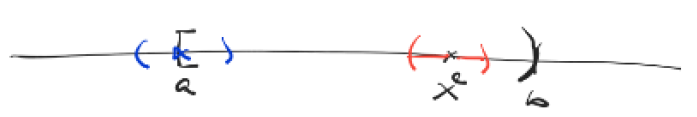
\includegraphics[width=0.7\linewidth]{figures/umgebung_beispiel_halboffenes_intervall}
            \label{fig:umgebung_beispiel_halboffenes_intervall}
        \end{figure}
        
        \item \( \ointerval{a-\varepsilon}{a+\varepsilon} \),  \( \varepsilon>0 \), ist eine Umgebung von \( a \).         
    \end{enumerate}
\end{beispiele*}
\begin{lemma}\label{offene_menge_umgebung_aller_elemente}
    Eine Teilmenge \( V\subset X \) eines topologischen Raumes \( (X,\mathcal{T}) \) ist offen \gdw für alle \( x\in V \) gilt: \( V \) ist Umgebung von \( x \).
\end{lemma}
\begin{proof}
    \begin{proofdescription}
        
        \item[\hin] Ist \( V \) offen, so erfüllt \( U=V \) für jedes \( x \) die Bedingung \( x\in U \) und \( U\subset V \) \timplies \( V \) ist Umgebung.
        \item[\rueck] Zu \( x\in V \) wähle \( U_x \) \sd \( x\in U_x \), \( U\subset V \). 
        Dann gilt \( V=\bigcup_{x\in U} U_x \) und das ist offen (nach \ref{topologie:unendliche_vereinigung}).
    \end{proofdescription}
    
    
\end{proof}
\begin{definition}[Konvergenz in topologischen Räumen] \label{konvergenz_in_topologischen_raeumen}\index{Konvergenz}
    Sei \( (X, \mathcal{T}) \) topologischer Raum.
    Sei \( (x_n)_{n\in \naturals} \) eine Folge in \( X \).
    Dann ist \( (x_n)_{n} \) \emph{konvergent mit Grenzwert \( x \)}, \( x_n\goesto x \) in \( (X, \mathcal{T}) \), falls es in jeder Umgebung \( V \) von \( x  \) ein \( N\in \naturals \) gibt, \sd \( x_n\in V\logicspace\forall n\geq N \).
    
\end{definition}

\begin{beispiele*}
    \begin{enumerate}
        \item In der Klumpentopologie konvergieren alle Folgen gegen jedes \( x\in X \).
        \item Mit unseren obigen Überlegungen folgern wir, dass Konvergenz in \( \reals \) im Sinn von \thref{konvergenz_in_topologischen_raeumen} mit Konvergenz, wie wir sie in der \diffcourse{1} kennengelernt haben.
    \end{enumerate}
\end{beispiele*}
\begin{lemma}\label{hausdorff_alle_grenzwerte_eindeutig}
    Sei \( (X,\mathcal{T}) \) toplogischer Raum. 
    Ist \( (X, \mathcal{T}) \) ein \emph{Hausdorff-Raum}, gibt es also zu je zwei Punkten \( x,y\in X \) mit \( x\neq y \) Umgebungen \( U \) von \( x \) und \( V \) von \( y \) mit \( U \cap V=\emptyset \), so ist der Grenzwert einer konvergenten Folge eindeutig.
\end{lemma}
\begin{proof}
    Seien \( x \) und \( y \) Grenzwert einer Folge \( (x_n)_n \).
    Angenommen \( x\neq y \), so wähle \( U \) Umgebung von \( x \), \( V \) Umgebung von \( y \) mit \( U\cap V=\emptyset \). 
    Dann gibt es (wegen der Konvergenz) \( N \in \naturals \) \sd \( x_n \in U \logicspace\forall n \geq N \) und \( M\in \naturals \) \sd \( x_n \in V \logicspace \forall n \geq M \). 
    Wiederspruch zu \( U\cap V = \emptyset \). 
\end{proof}
\begin{definition}\label{stetigkeit_in_topologischen_raeumen}\index{Stetigkeit}
    Seien \( (X, \mathcal{T}) \) und \( (Y,\tilde{\mathcal{T}}) \) topologische Räume. 
    Sei \( f\maps X\to Y \) eine Abbildung. 
    Dann heißt \( f \) \emph{stetig in \( a\in X \)}, falls es zu jeder Umgebung \( V \) von \( f(a)\in Y \) eine Umgebung \( U \) von \( a \) gibt, \sd \( f(U)\subset V \). 
    \( f \) heißt \emph{stetig} (auf \( X \)), falls \( f \) stetig in allen \( a\in X \) ist.
\end{definition}
\begin{bemerkung*}
    Wir werden später sehen, dass diese Definition für \( f\maps \reals\to\reals \) mit unserer Definition aus der \diffcourse{1} übereinstimmt (\( \varepsilon \)-\( \delta \)-Kriterium).
\end{bemerkung*}
\begin{figure}[H]
    \centering
    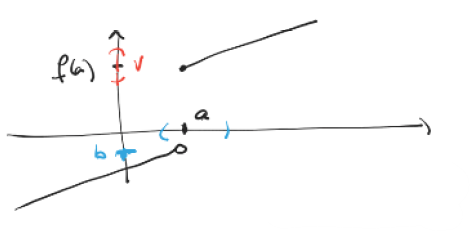
\includegraphics[width=0.6\linewidth]{figures/topologische_unstetigkeit_beispiel_aus_r}
    \caption*{\textcolor{Cyan}{Für jede Umgebung \( U \) von \( a \) gilt: \( f(U) \) enthält auch Punkte \( <b \), also außerhalb }\textcolor{OrangeRed}{\( V \)}}
    \label{fig:topologische_unstetigkeit_beispiel_aus_r}
\end{figure}
\begin{satz}\label{stetigkeit_in_topologischen_raeumen:urbildkriterium}
    Sei \( f\maps X\to Y \) Abbildung zwischen topologischen Räumen. 
    Dann ist \( f \) stetig auf \( X \) \gdw für jede offene Teilmenge \( V\subset Y \) das \emph{Urbild} \( \inverse{f}(V) \), also \( \Set{x\in X|f(x)\in V} \) offen in \( X \) ist.
\end{satz}
\begin{proof}
    \begin{proofdescription}
        
        \item[\hin] Sei \( f \) stetig vorausgesetzt.
        Sei \( V \) offen \( Y \). Ist das Urbild \( \inverse{f}(V) \) leer, sind wir fertig.
        
        Sei also \( a\in \inverse{f}(V) \). 
        Dann gibt es nach Voraussetzung eine Umgebung \( U \) von \( a \) \sd \( f(U)\subset V \). 
        Also gilt \( U \subset \inverse{f}(V)\). 
        Somit besitzt also jeder Punkt \( a\in \inverse{f}(V) \) eine Umgebung \( U \) mit \( U\subset \inverse{f}(V) \) und somit ist \( \inverse{f}(V) \) selbst Umgebung jedes seiner Elemente \( \overset{\ref{offene_menge_umgebung_aller_elemente}}{\implies} \inverse{f}(V)\) ist offen.

        
        \item[\rueck] Sei \( a\in X \) beliebig. Sei \( V \) eine Umgebung von \( f(a) \). Dann gibt es \( \tilde{V} \) offen mit \( f(a)\in \tilde{V} \) und \( \tilde{V}\subset V \). Nach Voraussetzung ist das Urbild \( U\definedas \inverse{f}(\tilde{V}) \) offen. \( U \) enthält \( a \), ist also Umgebung von \( a \) und es gilt \( f(U)=\tilde{V}\subset V \)\timplies \( f \) ist stetig in \( a \).
    \end{proofdescription}
    
\end{proof}
\begin{figure}[H]
    \centering
    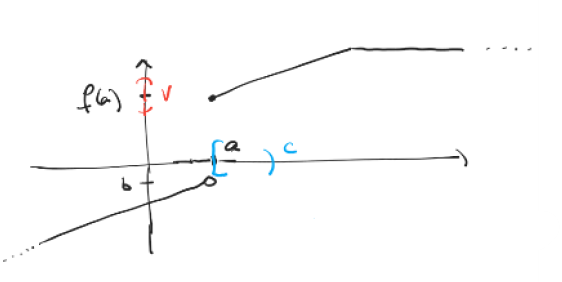
\includegraphics[width=0.8\linewidth]{figures/beispiel_urbild_offener_menge_unter_nicht_stetiger_abbildung_nicht_offen}
    \caption*{\textcolor{Cyan}{\( \inverse{f}(V)=\rinterval{a}{c} \) ist nicht offen in \( \reals \)}}
    \label{fig:beispiel_urbild_offener_menge_unter_nicht_stetiger_abbildung_nicht_offen}
\end{figure}
\begin{bemerkung*}
    Äquivalent: \( f \) ist genau dann stetig, wenn das Bild jeder abgeschlossen Menge abgeschlossen ist.
\end{bemerkung*}
\minisec{Vorsicht:}
Es ist immer Offenheit in \( X \) (\bzw \( Y \)) gemeint!

\minisec{Zur Veranschaulichung:}
Betrachtet man im Beispiel oben als Definitionsbereich \( X=\rinterval{a}{\infty} \), so ist die Funktion stetig! 
Dies ist konsistent, da \( \rinterval{a}{c} \) in \( X=\rinterval{a}{\infty} \) versehen mit der Standard-Topologie tatsächlich offen ist:
\begin{defsatz}
    Sei \( (X,\mathcal{T}) \) topologischer Raum. Sei \( \tilde{X}\subset X \) eine Teilmenge. Dann induziert \( \mathcal{T} \) auf \( \tilde{X}  \) eine Topologie, die sogenannte \emph{Teilraum-Topologie} vermöge
    \begin{align*}
        T_{\tilde{X}}\definedas \Set{U\cap \tilde{X}|U\in \mathcal{T}}.
    \end{align*}
    Den (einfachen) Beweis, dass dies in der Tat eine Topologie definiert, lassen wir weg.
\end{defsatz}

In unserem Beispiel ist \( X=\reals \), \( \tilde{X}=\rinterval{a}{\infty} \) und da \( \ointerval{a-\varepsilon}{c} \) offen in \( \reals \) ist (\( \varepsilon>0 \)), ist nach Definitionsbereich \( \rinterval{a}{c}=\ointerval{a-\varepsilon}{c}\cap \rinterval{a}{\infty} \) offen in \( \rinterval{a}{\infty} \).

Dies ist der tiefere Grund, weshalb man bei Funktionen den Raum, in dem sie ihre Werte annehmen (im Beispiel oben \( Y=\reals \)) angeben sollte, nicht ihr Bild.

Denn in \( Y =\ointerval{-\infty}{b}\cup \rinterval{f(a)}{\infty}\) wäre das Bild von \( \interval{a-\varepsilon}{c}\) \tforall \( \varepsilon>0 \) in der Tat abgeschlossen, denn sein Komplement
\begin{align*}
    Y\setminus (\rinterval{b-\delta}{b}\cup \rinterval{f(a)}{f(c)})=-\ointerval{-\infty
    }{b-\delta}\cup \ointerval{f(c)}{\infty}
\end{align*}
wäre offen.

Dagegen ist
\begin{align*}
    \reals\setminus (\rinterval{b-\delta}{b}\cup \rinterval{f(a)}{f(c)})=-\ointerval{-\infty
    }{b-\delta}\cup \rinterval{b}{f(a)}\cup\ointerval{f(c)}{\infty}
\end{align*}
für kein \( \delta>0 \) offen.

\begin{defsatz}
    Seien \( (X, \mathcal{T}_X) \)  und \( (Y,\mathcal{T}_Y) \) topologische Räume. Betrachte das \emph{kartesische Produkt} \( X\times Y=\Set{(x,y)|x\in X, y\in Y} \). Dann nennt man das System
    \begin{align*}
        T\definedas \Set{U\subset X\times X | U = \begin{aligned}[t] 
            \text{beliebige Vereinigung von Mengen der Form }\\
            V\times W, V\in \mathcal{T}_X, W\in \mathcal{T}_Y
        \end{aligned}}
    \end{align*}
    \emph{Produkttopologie}. Und dies definiert in der Tat eine Topologie auf \( X\times Y \).
\end{defsatz}
\begin{proof}
    \begin{proofdescription}
                
        \item[\ref{topologie:grundmengen}] klar
        \item[\ref{topologie:endlicher_schnitt}] \begin{align*}
            U&=\bigcup_{\alpha} U_\alpha\times W_\alpha\\
            V&=\bigcup_{\beta} \tilde{V}_\beta \times \tilde{W}_\beta\\
            U\cap V&= \bigcup_{\alpha, \beta} (\underbrace{V_\alpha\cap \tilde{V}_\beta}_{\text{offen in }X})\times(\underbrace{W_\alpha\cap \tilde{W}_\beta}_{\text{offen in }Y}).
        \end{align*}
        \item[\ref{topologie:unendliche_vereinigung}] \begin{align*}
            \bigcup_\rho \p*{\bigcup_\alpha V_\alpha^{(\rho)}\times W_\alpha^{(\rho)}}=\bigcup_{\rho,\alpha} V_\alpha^{(\rho)}\times W_{\alpha}^{(\rho)}.
        \end{align*}
    \end{proofdescription}    
\end{proof}

Wir kommen nun zu einer wichtigen Beispiel-Klasse für Topologien:
\begin{definition}\index{Metrik}
    Sei \( X \) eine Menge. Eine \emph{Metrik} auf \( X \) ist eine Abbildung
    \begin{align*}
        d\maps X\times X \to \reals
    \end{align*}
    mit den Eigenschaften
    \begin{eigenschaftenenumerate}
        \item \label{metrik:nicht_ausgeartet}\( \distance{x}{y}=0 \) \tiff \( x=y \) \enquote{\( d \) ist nicht ausgeartet.}
        \item \label{metrik:symmetrisch}\( \distance{x}{y}=\distance{y}{x}\logicspace\forall x,y \in X \) \enquote{\( d \) ist symmetrisch.}
        \item \label{metrik:dreiecksungleichung} \( \distance{x}{y}\leq \distance{x}{z}+\distance{z}{y} \logicspace\forall x,y,z\in X\) \enquote{Es gilt die Dreiecksungleichung.} 
    \end{eigenschaftenenumerate}
    Ein \emph{metrischer Raum} ist ein Tupel \( (X,d) \), wobei \( X \) eine Menge ist und \( d \) eine Metrik auf \( X \). Meist schreibt man nur \( X \), weil Missverständnisse ausgeschlossen sind.
\end{definition}
\begin{bemerkung*}
    Aus den Axiomen folgt auch
    \begin{align*}
        \distance{x}{y}\geq 0 \logicspace \forall x,y \in X,
    \end{align*}
    denn
    \begin{align*}
        0\explain{\ref{metrik:nicht_ausgeartet}}{=}\distance{x}{x}\explain{\triangle\text{-\Ungl}}{\leq}\distance{x}{y}+\distance{y}{x}\explain{\text{Symm.}}{=}2\distance{x}{y}.
    \end{align*}
\end{bemerkung*}
\begin{beispiele*}
    \begin{enumerate}[label=\rechtsklammer{\roman*}, ref=\rechtsklammer{\roman*}]
        \item \label{metrik:beispiele:r}\( \reals \), \( \distance{x}{y}=\abs{x-y} \).
        \item \label{metrik:beispiele:diskret}\( X \) Menge, \( \distance{x}{y}=\begin{cases}
            1 & x\neq y\\
            0 & x=y
        \end{cases}
         \), \enquote{triviale} oder \enquote{diskrete Metrik}.
         
         \item\label{metrik:beispiele:r_n} (aus \aglacourse{1}) \( \reals^n \), \( \distance{x}{y}=\sqrt{\sum_{i=1}^{n} (x_i-y_i)^2} \), \enquote{Euklidische Metrik}.
    \end{enumerate}
\end{beispiele*}
Eine Metrik misst den \emph{Abstand} zwischen zwei Punkten. 
Im zweiten Beispiel sind alle verschiedenen Punkte gleich weit von einander entfernt. 
Für \( n=1 \) stimmt \ref{metrik:beispiele:r_n} mit \ref{metrik:beispiele:r} überein. 
Mit \ref{metrik:beispiele:r_n} wird auch der Name der Dreiecksungleichung klar:
\begin{figure}[H]
    \centering
    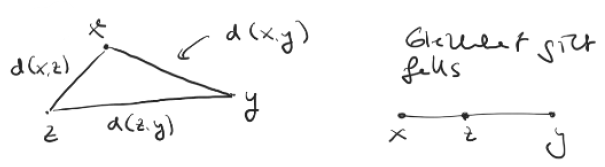
\includegraphics[width=0.8\linewidth]{figures/dreiecksungleichung_visualisierung}
    \label{fig:dreiecksungleichung_visualisierung}
\end{figure}
\begin{definition}\index{$\varepsilon$-Ball}
    Sei \( (X,d) \) ein metrischer Raum. Seien \( x\in X \), \( \varepsilon>0 \). Dann nennt man
    \begin{align*}
        B_\epsilon(x)\definedas\Set{y\in X| \distance{x}{y}<\varepsilon}
    \end{align*}
    den (offenen) \( \varepsilon \)-Ball um \( x \).
\end{definition}
\begin{beispiele*}
    \begin{enumerate}
        \item \( B_\varepsilon(x)=\ointerval{x-\varepsilon}{x+\varepsilon} \).
        \item \( B_\varepsilon(x)=\begin{cases}
            x & \varepsilon\leq 1 \\
            X & \varepsilon>1
        \end{cases}
         \)
         
        \item \( B_\varepsilon(x)= \) \raisebox{-2em}{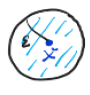
\includegraphics[width=0.1\linewidth]{figures/offener_ball_r_n}}
        
    \end{enumerate}
\end{beispiele*}
\begin{satz}\label{metrische_topologie}
    Sei \( (X,d) \) ein metrischer Raum. Dann wird durch
    \begin{align*}
        \mathcal{T}_d\definedas \Set{U\subset X|\forall x\in U\logicspace\exists\varepsilon>0\logicspace\text{\sd}\logicspace B_\varepsilon(x)\subset U}
    \end{align*}
    eine Topologie definiert.
\end{satz}
\begin{proof}
    Als Hausaufgabe.    
\end{proof}
\begin{bemerkungen}
    \begin{enumerate}
        \item \ref{standard-topologie} ist ein Spezialfall dieser Aussage
        \item Die \enquote{offenen} \( \varepsilon \)-Bälle sind tatsächlich offen: Zu \( y\in B_\varepsilon(x) \) wähl \( \tilde{\varepsilon}\definedas \varepsilon-\distance{x}{y}>0 \).
        \begin{figure}[H]
            \centering
            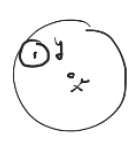
\includegraphics[width=0.3\linewidth]{figures/offene_baelle_sind_offen}
            \label{fig:offene_baelle_sind_offen}
        \end{figure}
        Dann ist \( B_{\tilde{\varepsilon}}(y)=\Set{z|\distance{y}{z}<\tilde{\varepsilon}} \subset B_\varepsilon(x)\). Denn für alle \( z\in B_{\tilde{\varepsilon}}(y) \) ist
        \begin{align*}
            \distance{x}{z}\begin{aligned}[t] 
                &\leq \distance{x}{y}+\distance{y}{z}<\distance{x}{y}+\tilde{\varepsilon}\\
                &=\distance{x}{y}+\varepsilon-\distance{x}{y}=\varepsilon
            \end{aligned}
        \end{align*}
        
        \item Bezüglich der diskreten Metrik ist \emph{jede} Teilmenge offen.
        \item Die Klumpentopologie wird nicht von einer Metrik erzeugt (wenn \( X \) mehr als \( 1 \) Element enthält).
        \begin{proof}
            Seien \( x,y\in X \), \( x\neq y \). Angenommen \texists Metrik \( d \).
            \begin{align*}
                \implies &\distance{x}{y}\neq 0\implies \distance{x}{y}=c>0\\
                \implies &B_c(x)\text{ ist offen.}\\
                \underset{\text{\scshape{VOR}}}{\implies} &B_c(x)=\emptyset \text{ oder } =X\\
                \implies &B_c(x)=X
            \end{align*}
            \contra, da \( y\notin B_c(x) \).
            
        \end{proof}
        
        \item \label{metrischer_raum_ist_hausdorffsch} Ein metrischer Raum ist hausdorffsch. \tto HA\@.
        
    \end{enumerate}
\end{bemerkungen}
Wir formulieren nun Konvergenz und Stetigkeit für metrische Räume:
\begin{bemerkungen}
    Sei \( (X,d) \) metrischer Raum.
    \begin{enumerate}
        \item {}[\thref{umgebung_in_topologischen_raeumen}]\label{umgebung_in_metrischen_raeumen} \( V\subset X \) heißt Umgebung von \( x\in X \), falls es \( \varepsilon >0 \) gibt \sd \( B_\varepsilon(x)\subset U \).
        \item {}[\thref{konvergenz_in_topologischen_raeumen}]\label{konvergenz_in_metrischen_raeumen} \( (x_n)_n \) konvergiert mit Grenzwert \( x \), falls es zu jedem \( \varepsilon>0 \) ein \( N\in \naturals \) gibt \sd \( x_n\in B_\varepsilon(x)\logicspace\forall n\geq N \).
        \item {}[\thref{stetigkeit_in_topologischen_raeumen}]\label{stetigkeit_in_metrischen_raeumen} Sei \( (Y,\tilde{d}) \) weiterer metrischer Raum, \( f\maps X \to Y \) eine Abbildung. Dann ist \( f \) stetig \( a \) \gdw:
        \begin{align*}
            \forall\varepsilon>0\logicspace\exists \delta>0\logicspace\text{\sd} f(B_\delta(a))\subset B_\varepsilon(f(a)).
        \end{align*}
    \end{enumerate}
\end{bemerkungen}
\begin{bemerkungen*}
    \begin{enumerate}
        \item \ref{stetigkeit_in_metrischen_raeumen} ist das \( \varepsilon \)-\( \delta \)-Kriterium.
        \item Die Einschränkung auf \( \varepsilon \)-Bälle in \ref{konvergenz_in_metrischen_raeumen} und \ref{stetigkeit_in_metrischen_raeumen} (statt allgemeiner Umgebungen) ist keine echte Einschränkung: Gilt etwas für all Umgebungen, so speziell auch für \( \varepsilon \)-Bälle.
        
        Und gilt eine Inklusion für alle \( \varepsilon \)-Bälle (etwa \( x_n\in B_\varepsilon(x)\logicspace\forall n \geq N(\varepsilon) \)), so auch für beliebige Umgebungen \( U \) von \( x \), da es immer einen \( \varepsilon \)-Ball \( B_\varepsilon(x) \) gibt, der ganz in \( U \) enthalten ist.
    \end{enumerate}
\end{bemerkungen*}
\begin{beispiele}
    \begin{enumerate}
        \item \( \reals^m \) mit der Euklidischen Metrik. \( (x_n)_{n\geq 1} \) Folge in \( \reals^m \), also \( n\mapsto x_n=(x_n^{(1)},\ldots, x_n^{(m)})\in \reals^m \).
        \item \( x_n=\p*{ \frac{1}{n}\Cos+{n},\frac{1}{n}\Sin+{n},a,\ldots,a } \)
        \begin{behauptung*}
            \( x_n\goesto (0,0,a,\ldots,a)\defines x \).
        \end{behauptung*}
        \begin{proof}
            Sei \( \varepsilon>0 \). Es gilt
            \begin{align*}
                &\distance{x_n}{x}^2 \begin{aligned}[t] 
                    &=\sum\limits_{i=1}^{m} (x_n^{(i)}-x^{(i)})^2\\
                    &=\p*{ \frac{1}{n}\Cos+{n}-0 }^2+\p*{ \frac{1}{n}\Sin+{n}-0 }^2+(a-a)^2+\cdots +(a-a)^2\\
                    &=\frac{1}{n^2}(\Cos+{n}^2+\Sin+{n}^2)=\frac{1}{n^2}
                \end{aligned}\\
                \implies &\distance{x_n}{x}=\frac{1}{n}\\
                \implies &\distance{x_n}{x}<\varepsilon\logicspace\forall n\geq N\text{ mit } N>\frac{1}{\varepsilon}\\
                \implies &x_n \in B_\varepsilon(x) \logicspace\forall n \geq N.
            \end{align*}            
        \end{proof}
        
        \item \( X=\stetigefunktionen(\interval{a}{b}) \), \( \distance{f}{g}\definedas \supnorm{f-g} \) mit \( \supnorm{f-g}=\sup_{x\in \interval{a}{b}}\abs{f(x)-g(x)} \).
        \begin{enumerate}[label=\textbf{\arabic*. Beh}]
            \item \( d \) ist eine Metrik auf \( X \).
            \begin{proof}
                \begin{proofdescription}
                    
                    \item[\ref{metrik:nicht_ausgeartet}:]
                    \begin{align*}
                        &\sup_{x\in \interval{a}{b}}\abs{f(x)-g(x)}=0\\
                        \iff &\abs{f(x)-g(x)}=0\logicspace\forall x\\
                        \iff f(x)=g(x)\logicspace\forall x.
                    \end{align*} 
                    
                    \item[\ref{metrik:symmetrisch}:]
                    \begin{align*}
                        &\abs{f(x)-g(x)}=\abs{g(x)-f(x)}\logicspace\forall x\\
                        \implies &\distance{f}{g}=\distance{g}{f}.
                    \end{align*} 
                    \item[\ref{metrik:dreiecksungleichung}:]
                     \begin{align*}
                         &\abs{f(x)-g(x)}\begin{aligned}[t] 
                             &=\abs{f(x)-h(x)+h(x)-g(x)}\\
                             &\explain{\triangle-\text{\Ungl für \( \abs{\cdot} \) auf \( \reals \)}}{\leq} \abs{f(x)-h(x)}+\abs{h(x)-g(x)}
                         \end{aligned}\\
                         \implies& \triangle\text{-\Ungl für \( d \)}.
                     \end{align*}
                \end{proofdescription}
                
            \end{proof}
            
            \item \( (f_n)_n\subset \stetigefunktionen(\interval{0}{1}) \), \( f_n(x)=x^n \), konvergiert nicht (\vgl \diffcourse{1}).
            \begin{proof}
                Wir wissen aus der \diffcourse{1}, dass wenn Konvergenz vorliegt, der Grenzwert gleich dem punktweisen Grenzwert ist. Dieser ist
                \begin{align*}
                    f(x)=\begin{cases}
                        1 & x=1\\
                        0 & \text{sonst}
                    \end{cases}.
                \end{align*}
                Aber
                \begin{align*}
                    \sup_{x\in \interval{0}{1}}\abs{f_n(x)-f(x)}=\sup_{x\in \rinterval{0}{1}}\abs{x^n}=1.
                \end{align*}
            \end{proof}
            
        \end{enumerate}
        \item \( X=\stetigefunktionen(\interval{0}{1}) \), \( \distance{f}{g}=\Integrate{\abs{f(x)-g(x)}}{x,0,1} \).
        \begin{enumerate}[label=\textbf{\arabic*. Beh}]
            
            \item \( d \) ist eine Metrik auf \( \stetigefunktionen(\interval{0}{1}) \).
            \begin{proof}
                HA\@.
            \end{proof}
            
            \item \( (f_n)_n\subset \stetigefunktionen(\interval{0}{1}) \), \( f_n(x)=x^n \) konvergiert, und zwar gegen \( f(x)=0\logicspace\forall x \).
            \begin{proof}
                \begin{align*}
                    &\Integrate{\abs*{f_n(x)-0}}{x,0,1}%=\Integrate{x^n}{x,0,1}=\frac{1}{n+1}\evaluatebetween{x^{n+1}}{x}{0}{1}=\frac{1}{n+1}\\ 
                    \implies &\distance{f_n}{f}=\frac{1}{n+1}<\varepsilon\logicspace\forall n\geq N \text{ mit } N \geq \frac{1}{\varepsilon}.
                \end{align*}
            \end{proof}
            
        \end{enumerate}
        
    \end{enumerate}
\end{beispiele}
 sie
% !TEX root = ./Vorlesungsmitschrift DIFF 2.tex  
\lecture{Do 23.04. 10:15}{} Bevor wir uns mit offenen und abgeschlossenen Mengen und
sogenannten vollständigen metrischen Räumen näher befassen, beweisen wir noch zwei
nützliche Lemmata zu Konvergenz und Stetigkeit:

\begin{lemma}\label{konvergenz_abstand_ist_nullfolge}
    \( (X,d) \) sei metrischer Raum.

    Eine Folge \( (x_n)_n \) in \( X \) konvergiert in \( X \) gegen \( a\in X \)
    \begin{align*}
        \iff (\distance{x_n}{a})_n \text{ ist Nullfolge}\logicspace(\text{in } \reals).
    \end{align*}
\end{lemma}
\begin{proof}
    \begin{align*}
        \distance{x_n}{a}=\abs{\distance{x_n}{a}-0}.
    \end{align*}
    Also ist
    \begin{align*}
        \distance{x_n}{a}<\varepsilon\iff \abs{\distance{x_n}{a}-0}<\varepsilon.
    \end{align*}
    
\end{proof}
\begin{lemma}\label{stetigkeit:folgenkonvergenzkriterium}
    Seien \( (X,d_x) \) und \( (Y, d_y) \) metrische Räume, \( f\maps X\to Y \) eine Abbildung. 
    Dann gilt:

    \( f \) ist in \( a\in X \) stetig \tiff für jede Folge \( (a_n)_n \) mit \( a_n\goesto a \) in \( X \) gilt
    \begin{align*}
        \lim\limits_{n \goesto \infty}  f(a_n)=f(\underbrace{\lim a_n}_{=a}).
    \end{align*} 
    \begin{notation*}
        \begin{align*}
            \lim\limits_{x \goesto a} f(x)=f(a).
        \end{align*}
    \end{notation*}
    
\end{lemma}
\begin{proof}
    \begin{proofdescription}
        
        \item[\hin] Sei das \( \varepsilon \)-\( \delta \)-Kriterium erfüllt (\ref{stetigkeit_in_metrischen_raeumen}).
        Sei \( (x_n)_n \) Folge in \( X \) mit \( x_n\goesto a \) in \( X \). Sei \( \varepsilon>0 \). Dann \texists \( \delta>0 \) \sd
        \begin{align*}
            d_Y(f(x),f(a))<\varepsilon\logicspace\forall x\in B_\delta(a)\subset X.
        \end{align*} 
        Wegen der Konvergenz \texists \( N=N(\delta) \) \sd
        \begin{align*}
            &x_n\in B_\delta(a) \logicspace\forall n\geq N\\
            \implies &f(x_n)\in B_\varepsilon(f(a))\subset Y \logicspace \forall n\geq N.
        \end{align*}
        Also gilt \( f(x_n)\goesto f(a) \).
        \item[\rueck] Gelte \( \lim_{x \goesto a} (x)=f(a) \).
        
        Angenommen, das \( \varepsilon \)-\( \delta \)-Kriterium wäre verletzt. Dann gäbe es \( \varepsilon>0 \) \sd für \emph{alle} \( \delta>0 \) ein \( x\in X \) existierte \sd
        \begin{align*}
            x\in B_\delta(a)\logicspace \begin{aligned}[t] 
                &\text{aber} \logicspace f(x)\notin B_\varepsilon(f(a))\\
                &\text{also} \logicspace d_y(f(x), f(a)) \geq \varepsilon.
            \end{aligned}
        \end{align*}
        Insbesondere gäbe es zu \( \delta=\frac{1}{n} \) ein solches \( x \), nennen wir es \( x_n \). Dann gilt für alle \( n \): \( \distance{x_n}{a}<\frac{1}{n} \), aber \( d_y(f(x_n),f(a))\geq \varepsilon \), somit \( x_n\goesto a \) aber \( f(x_n)\not\goesto f(a) \) (wegen \ref{konvergenz_abstand_ist_nullfolge}).
    \end{proofdescription}
    
    
\end{proof}
\section{Charakterisierung topologischer Grundbegriffe in metrischen Räumen}
\begin{lemma}\label{abgeschlossenheit:folgenkonvergenzkriterium}
    Sei \( (X,d) \) metrischer Raum. 
    Dann ist \( A\subset X \) abgeschlossen \tiff für jede Folge \( (a_n)_n \), \( a_n\in A \), die in \( X \) konvergiert, gilt:
    \begin{align*}
        \lim\limits_{n \goesto \infty} a_n\in A.
    \end{align*}
\end{lemma}
\begin{proof}
    \Obda \( \emptyset\neq A\neq X \).
    
    \begin{proofenumerate}
        
        \item[\hin] Sei \( (a_n)_n \), \( a_n\in A \), konvergent in \( X \).
         Sei \( a=\lim a_n \). Angenommen \( a\notin A \). Nach Voraussetzung ist \( X\setminus A \) offen, also ist \( X\setminus A \) Umgebung von \( a \) \timplies \texists \( N \) \sd
         \begin{align*}
             a_n \in X\setminus A \logicspace \forall n\geq N \logicspace (\text{wegen Konvergenz})
         \end{align*}
         \contra zu \( a_n\in A \).
         
         \item[\rueck] Wir zeigen, dass \( X\setminus A \) offen ist.
         Sei also \( b\in X \setminus A \). Es gibt \( \varepsilon>0 \) \sd \( B_\varepsilon(b)\cap A=\emptyset \), also \( B_\varepsilon(b)\subset X\setminus A \). 
         
         Denn angenommen es gibt kein solches \( \varepsilon \). 
         Dann gilt für \emph{alle} \( \varepsilon>0 \):
         \( B_\varepsilon(b)\cap A\neq \emptyset \), also kann man zu jedem \( k\geq 1 \) ein \( x_k\in A \) finden mit \( \distance{x_k}{ b}<\frac{1}{k}=\varepsilon \).
         \begin{align*}
             \implies x_k=b\underset{\text{\textsc{Vor}}}{\implies} b\in A.
         \end{align*}
         \contra Wiederspruch zu \( b\in X\setminus A \).

         Also gibt es ein solches \( \varepsilon>0 \), also ist \( X\setminus A \) offen.
    \end{proofenumerate}
    
\end{proof}
\begin{definition}\index{Randpunkt}
    Sei \( (X,d) \) metrischer Raum, \( M\subset X \). Ein Punkt \( y\in X \) heißt \emph{Randpunkt} von \( M \), falls in jeder Umgebung von \( y \) sowohl Punkte von \( M \) als auch \( X\setminus M \) liegen.
\end{definition}
\begin{notation*}
    \( \randpunkte M=\Set{\text{Randpunkte von \( M \)}} \)
\end{notation*}
\begin{beispiel*}[\( \reals^n \), \( d_{\text{Eukl.}} \)]
   Kugel im \( \reals^m \):
   \begin{align*}
       K^n&\definedas \Set{x\in \reals^n| \norm{x-0}_\text{E}\leq R}\subset \reals^n\\
       \intertext{Sphäre:}
       \randpunkte K^n &=\Set{x\in \reals^n|\norm{x}_\text{E}= R}=S^{n-1}
   \end{align*} 
\end{beispiel*}

\begin{beispiel*}
    \( \rationals\subset \reals \). \( \randpunkte \rationals =\reals\).
\end{beispiel*}
\begin{satz}
    Sei \( (X,d) \) metrischer Raum. Sei \( M\subset X \). Dann gilt
    \begin{enumerate}
        \item \label{interior_ist_offen}\( M\setminus \randpunkte M \) ist offen.
        \item \label{abschluss_ist_geschlossen}\( M\cup \randpunkte M \) ist abgeschlossen.
        \item \label{rand_ist_geschlossen}\( \randpunkte M \) ist abgeschlossen.
    \end{enumerate}
\end{satz}
\begin{proof}
    \begin{proofdescription}
        
        \item[\ref{interior_ist_offen}:] \( a\in M\setminus \randpunkte M \) \timplies \texists \( \varepsilon>0 \) \sd \( B_\varepsilon(a)\cap X\setminus M = \emptyset \). Für dieses gilt auch \( B_\varepsilon\cap \randpunkte M=\emptyset\) (denn angenommen \texists \( y\in B_\varepsilon(a)\cap \randpunkte M \),  dann wäre (da \( y\in \randpunkte M \) und \( B_\varepsilon(a) \) eine Umgebung von \( y \)) \( B_\varepsilon(a)\cap (X\setminus M)\neq \emptyset \) \contra \textsc{VOR}).
        
        Also gilt \( B_\varepsilon(a)\subset M\setminus \randpunkte M \) \timplies \Beh.
        \item[\ref{abschluss_ist_geschlossen}:] Es gilt \( \randpunkte M=\randpunkte{X\setminus M} \) (nach Definition), \( (X\setminus M)\setminus \randpunkte{X\setminus M} \) ist offen nach \ref{interior_ist_offen} \timplies \begin{align*}
            X\setminus ((X\setminus M)\setminus \randpunkte{X\setminus M})\explain{\text{Manipulation mit Mengen}}{=}(X\setminus(X\setminus M))\cup \randpunkte {X\setminus M}=M\cup \randpunkte M
        \end{align*}
        ist offen.
        \begin{figure}[H]
            \centering
            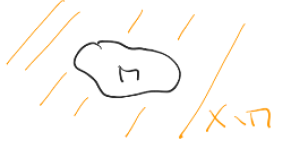
\includegraphics[width=0.5\linewidth]{figures/menge_und_komplement}
            \label{fig:menge_und_komplement}
        \end{figure}
        \item[\ref{rand_ist_geschlossen}:]
        \begin{align*}
            &\randpunkte M=(M\cup \randpunkte M)\setminus (M\setminus \randpunkte M)\\
            \implies &X\setminus \randpunkte M=\underbrace{X\setminus(\underbrace{M\cup \randpunkte M}_{\text{(abgeschl.\ nach \ref{abschluss_ist_geschlossen})}})}_{\text{offen}}\cup (\underbrace{M\setminus \randpunkte M}_{\text{offen nach \ref{interior_ist_offen}}}).
        \end{align*} 
    \end{proofdescription}
\end{proof}

\begin{notation*}
    Sei \( M\subset X \).
    \begin{align*}
        \inneres{M}&\definedas M\setminus \randpunkte M\text{ heißt das \emph{Innere} von \( M \).}\\
        \abschluss{M}&\definedas M\cup \randpunkte M\text{ heißt der \emph{Abschluss} von \( M \).}
    \end{align*}
\end{notation*}
Nach \ref{abgeschlossenheit:folgenkonvergenzkriterium} können wir \( \abschluss{M} \) konstruieren, indem wir zu \( M \) noch alle Grenzwerte von Folgen \( (x_n)_n \), \( x_n\in M \), die in in \( X \) konvergieren, hinzunehmen.
\begin{beispiel*}
    \( M=\rinterval{a}{b} \), \( \abschluss{M}=\interval{a}{b} \).
\end{beispiel*}
\begin{bemerkung*}[als Hausaufgabe]
    \begin{align*}
        M&\subset X \text{ offen} \iff M\cap \randpunkte M=\emptyset.\\
        M&\subset X \text{ abgeschlossen} \iff \randpunkte M \subset M.
    \end{align*}
    
\end{bemerkung*}
\section{Vollständigkeit}
\begin{definition}\index{Cauchy-Folge}
    Sei \( (X,d) \) ein metrischer Raum. Eine Folge \( (y_n)_n \subset X\) heißt \emph{Cauchy-Folge}, falls gilt
    \begin{align*}
        \forall \varepsilon>0 \logicspace \exists N\in \naturals \logicspace\text{\sd}\logicspace \distance{y_n}{ y_m}<\varepsilon \logicspace \forall n,m\geq N.
    \end{align*} 
\end{definition}
\begin{lemma}
    Sei \( (X,d) \)  ein metrischer Raum. Eine konvergente Folge in \( X \)  ist eine \emph{Cauchy-Folge}.
\end{lemma}
\begin{proof}
    Sei \( (y_n)_n \)  konvergente Folge mit Grenzwert \( y \) (eindeutig wegen \ref{metrischer_raum_ist_hausdorffsch} und \ref{hausdorff_alle_grenzwerte_eindeutig}). Sei \( \varepsilon>0 \).

    Dann gibt es \( N\in \naturals  \) \sd \( \distance{y_m}{ y}<\varepsilon \logicspace  \forall m\geq N\).
    \begin{align*}
        \implies \distance{y_n}{y_m}\underset{\triangle}{\leq}\distance{y_n}{y}+\distance{y}{y_m}<\epsilon \logicspace \forall n,m\leq N.
    \end{align*}   
\end{proof}
\begin{bemerkung*}
    Nicht jede Cauchy-Folge konvergiert:
    \begin{beispiel*}[\((\rationals, \abs{\cdot} )\)]
        \( y_{n+1}=\frac{1}{2}y_n+\frac{1}{y_n} \), \( y_0=1 \). 
    \end{beispiel*}
    \begin{checkenvironment*}
        Es gilt für \( n\geq 1 \)
        \begin{align*}
            \interval{\frac{1}{y_{n+1}}}{y_{n+1}}\subset \interval{\frac{1}{y_n}}{y_n} \label{eq:cauchy_folge_konvergiert_nicht:beispiel:intervallschachtelung}\tag{\(*\)}
        \end{align*} 
        und für \( l_n\definedas y_n-\frac{1}{y_n} \) 
        \begin{align*}
            &l_{n+1}\leq\frac{1}{4y_{n+1}}l_n^2\leq \frac{1}{4}l_n^2\tag{\(**\)}\label{eq:cauchy_folge_konvergiert_nicht:beispiel:abstand_nullfolge}\\
            \implies &\distance{y_n}{y_m}=\abs{y_n-y_m} \explain{\substack{\text{\Obda\ }m\geq n\\\implies y_m\in \interval{\frac{1}{y_n}}{y_n} \text{ wg.\ \eqref{eq:cauchy_folge_konvergiert_nicht:beispiel:intervallschachtelung}}}}{\leq}\abs{y_n-\frac{1}{y_n}}=l_n\explain{\text{wg.\ \eqref{eq:cauchy_folge_konvergiert_nicht:beispiel:abstand_nullfolge}}}{\goesto} 0.
        \end{align*}
        \( \rationals \subset \reals  \)  und somit \( (y_n)_n \subset \reals \).
        In \( \reals \) konvergiert jede Cauchy-Folge.
        Nennen wir den Grenzwert \( a\in \reals \). Es gilt dann
        \begin{align*}
            \underbrace{y_{n+1}}_{\goesto a}=\underbrace{\frac{1}{2}y_n}_{\frac{1}{2}a}+\underbrace{\frac{1}{y_n}}_{\frac{1}{a}},
        \end{align*} 
        also \( a^2=2\). Aber \( \sqrt{2}\notin \rationals \).
    \end{checkenvironment*}
    
\end{bemerkung*}
\begin{definition}\index{Vollständiger metrischer Raum}
    Ein metrischer Raum, in dem jede Cauchy-Folge konvergiert heißt \emph{vollständig}.
\end{definition}
\begin{beispiele}
    \begin{enumerate}
        
        \item \label{r_ist_vollstaendig} \( \reals ,\abs{\cdot} \) ist vollständig (\diffcourse{1}).
        \item \label{integral_metrischer_raum_ist_nicht_vollstaendig} \( (\stetigefunktionen(\interval{a}{b} ,\reals), d_{L^1})\) mit \( d_{L^1}(f,g)=\Integrate{\abs{f(t)-g(t)}}{t,a,b}\) (\vgl HA Blatt 1, A1) ist \emph{nicht} vollständig. 
        \item \( (\stetigefunktionen(\interval{a}{b},\reals ), d_{\sup})\), mit
        \begin{align*}
            d_{\sup}=\supnorm{f-g}=\sup_{t\in \interval{a}{b}}\abs{f(t)-g(t)},
        \end{align*}
        ist vollständig.
        Den Beweis führen wir später allgemeiner.
    \end{enumerate}
    

\end{beispiele}
Zunächst einige 
\section{Betrachtungen in vollständigen metrischen Räumen}

\begin{definition}\index{Beschränktheit}
    Sei \( (X,d)\) metrischer Raum, \( M\subset X\),
    \begin{align*}
        \diameter{M}\definedas \sup_{x,y\in M}\distance{x}{y}\logicspace \text{\enquote{Durchmesser} (englisch \enquote{diameter})}.
    \end{align*}
    \( M \) heißt \emph{beschränkt}, falls \( \diameter{M}<\infty \).
\end{definition}
\begin{bemerkung*}
    \( M\) ist beschränkt \tiff \texists \( R\geq 0\)  und \( a\in X\) \sd \( M\subset B_R(a)\) 
    \begin{figure}[H]
        \centering
        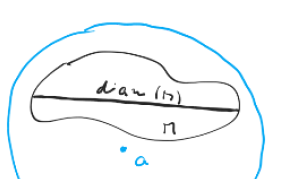
\includegraphics[width=0.5\linewidth]{figures/beschraenkte_menge_in_ball}
        \label{fig:beschraenkte_menge_in_ball}
    \end{figure}   
\end{bemerkung*}
\begin{beispiel*}
    \( \diameter{\rinterval{a}{b}}=b-a\)
\end{beispiel*}
\begin{satz}[Schachtelungsprinzip]\index{Schachtelungsprinzip}
    Sei \( (X,d)\) ein \emph{vollständiger} metrischer Raum und sei \( A_0\subset A_1\subset A_2\subset \cdots\).
    Eine Familie nicht-leerer abgeschlossener Teilmengen von \( X\) mit
    \begin{align*}
        \diameter{A_k}\goesto 0 \logicspace (\text{in }\reals)\logicspace \text{für } k\goesto \infty. 
    \end{align*} 
    Dann gibt es genau einen Punkt \( a\in X\) der in \emph{allen} \( A_k\) liegt.
\end{satz}
\begin{proof}
    \begin{proofdescription}
        \item[Eindeutigkeit:] Angenommen \texists \( x\neq y\)  mit \( x\in A_k \logicspace \forall k\)  und \( y\in A_k \logicspace \forall k\). Dann kann \( \diameter{A_k}\) keine Nullfolge sein, da \( \distance{x}{y}\neq 0\).
        \item[Existenz:] Wähle \( x_n\in A_n\). Dann ist \( (x_n)_n\)  eine Cauchy-Folge, denn
        \begin{align*}
            \distance{x_n}{x_m}\leq \diameter-{A_N} \logicspace \text{für }n,m\geq N 
        \end{align*} 
        \begin{figure}[H]
            \centering
            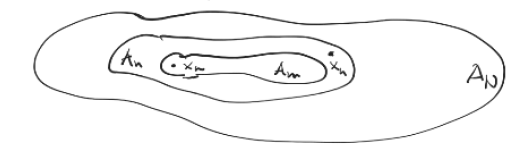
\includegraphics[width=0.5\linewidth]{figures/schachtelungsprinzip}
            \caption*{\( \distance{x_n}{x_m}\leq \diameter-{A_N}\) für \( \)    }
            \label{fig:schachtelungsprinzip}
        \end{figure}
        \begin{align*}
            \explain{\text{Vollständigkeit}}{\implies}x_n \goesto x \logicspace \text{in } X,
        \end{align*}
        Da \( x_n\in A_k\logicspace \forall n\geq k\), folgt mit \ref{abgeschlossenheit:folgenkonvergenzkriterium}: \( x\in A_k\logicspace \forall k\). 
    \end{proofdescription}
\end{proof}
Ein sehr wichtiger Satz, der viele Anwendungen hat ist der folgende:
\begin{satz}[Banach'scher Fixpunktsatz]\index{Banach'scher Fixpunktsatz}
    Sei \( (X,d_X)\) ein \emph{vollständiger} metrischer Raum. Sei \( M\subset X\) eine \emph{abgeschlossene} Teilmenge und \( \Phi\maps M\to X\) eine Abbildung mit \( \Phi(M)\subset M\) und es gebe \( 0\leq L<1\) \sd
    \begin{align*}
        d_X(\Phi(x),\Phi(y))\leq L d_X(x,y)\logicspace\forall x,y\in M\logicspace (\text{\enquote{\( \Phi\) ist Kontraktion}}).
    \end{align*}
    Dann gibt es genau ein \( t_*\) \sd \( \Phi(t_*)=t_*\). Ein solches \( t_*\) heißt \emph{Fixpunkt} von \( \Phi\). 
\end{satz}
\begin{beispiel*}
    \begin{figure}[H]
        \centering
        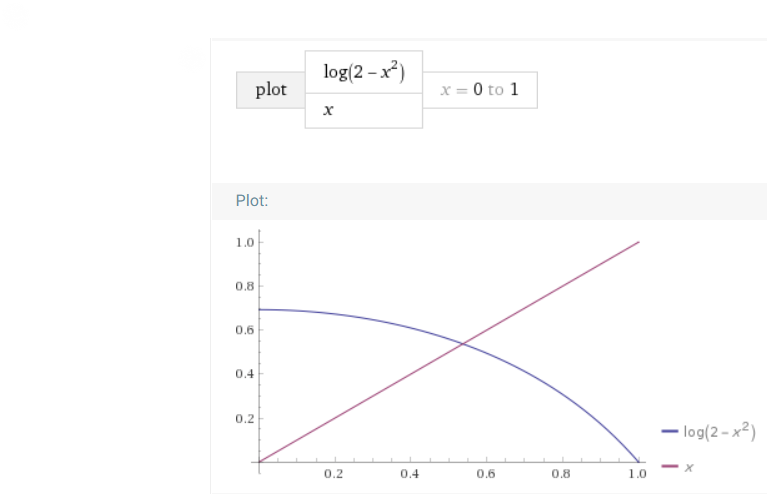
\includegraphics[width=0.5\linewidth]{figures/fixpunkt_beispiel}
        \caption*{\( X=\reals \), \( M=\interval{0}{1} \), \( \log(2-x^2)\), (WolframAlpha)}
        \label{fig:fixpunkt_beispiel}
    \end{figure}
\end{beispiel*}
\begin{proof}
    \begin{proofdescription}
        \item[Eindeutigkeit:] Seien \( \Phi(t_*)=t_*\), \( \Phi(\tilde{t}_*)=\tilde{t}_* \). Dann gilt
        \begin{align*}
            \distance{t_*}{\tilde{t_*} }\begin{aligned}[t]
                &=\distance{\Phi(t_*)}{\Phi(\tilde{t}_*)}\\
                &\leq \distance{t_*}{\tilde{t_*} }
            \end{aligned}
        \end{align*} 
        Da \( L<1\) ist, folgt \( \distance{t_*}{\tilde{t_*}=0 }\), also \( t_*=\tilde{t_*} \).
        \item[Existenz:] Wir betrachten die Folge \( x_0\in M\) beliebig, \( x_n\definedas \Phi(x_{n-1})\) für \( n\geq 1\).
        \begin{behauptung*}
            \( (x_n)_n\) konvergiert in \( M\)  und zwar gegen de Fixpunkt.
        \end{behauptung*}
        \begin{subproof}
            \begin{itemize}
                \item \( (x_n)_n\) ist Cauchy-Folge:
                \begin{align*}
                    \distance{\equalto{\Phi(x_n)}{x_{n+1}}}{\equalto[Bigg]{\Phi(x_{n-1})}{x_n}}\leq L \distance{x_n}{x_{n-1}}\logicspace \forall n\geq 1.
                \end{align*}
                Iteration liefert
                \begin{align*}
                    \distance{x_{n+1}}{x_n}\leq L^2 \distance{x_{n-1}}{x_{n-2}}\leq \cdots \leq L^n \distance{x_1}{x_0}.
                \end{align*}
                Zudem gilt
                \begin{align*}
                    \distance{x_{n+k}}{x_n}\begin{aligned}[t]
                        &\underset{\triangle}{\leq}\begin{aligned}[t]
                            &\distance{x_{n+k}}{x_{n+k}-1}\\
                            &+\distance{x_{n+k-1}}{x_{n+k-2}}\\
                            &\vdots\\
                            &+\distance{x_{n+1}}{x_n}
                        \end{aligned}\\
                        &\leq (\underbrace{L^{n+k-1}+L^{n+k-2}+\cdots+L^n}_{\mathclap{=L^n \sum_{r=0}^{k-1} L^r\leq L^n \sum_{r=0}^{\infty} L^r\explain{\text{geom.\ Reihe (\( L<1\))}}{=}\frac{L^n}{1-L}}})\distance{x_1}{x_0}
                    \end{aligned}
                \end{align*}
                \timplies (wegen \( L<1\)) \Beh.
                
                \item Da \( X\) vollständig ist, konvergiert \( (x_n)_n\). Setze \( t_*=\lim\limits_{n \goesto \infty} x_n\).
                \item Da \( M\) abgeschlossen ist, ist \( t_*\in M\) nach \ref{abgeschlossenheit:folgenkonvergenzkriterium}.
                \item \( t_*\) ist der gesuchte Fixpunkt:
                \begin{align*}
                    t_*=\lim\limits_{n \goesto \infty} x_n=\lim\limits_{n \goesto \infty} \Phi(x_{n-1})\explain{\text{Kontraktionen sind stetig und \ref{stetigkeit:folgenkonvergenzkriterium}}}{=}\Phi(t_*)
                \end{align*} 
            \end{itemize}
        \begin{figure}[H]
            \centering
            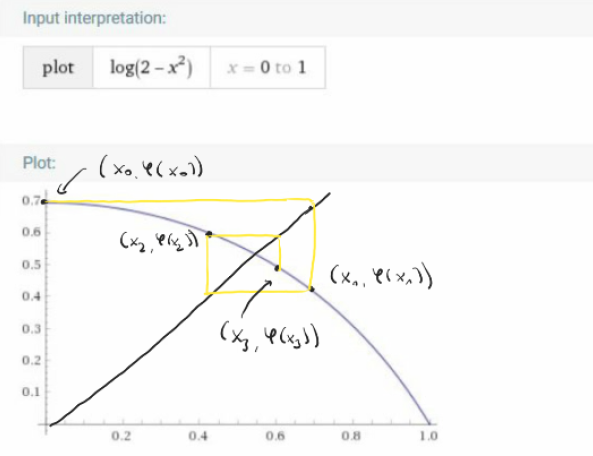
\includegraphics[width=0.6\linewidth]{figures/fixpunktsatz_beweis_existenz}
            \caption*{\( x_0=0\), \( x_1\Ln+{2-(\Ln{2})^2}\approx 0,42\), \( x_3\approx 0,60\), \( x_4\approx 0,49\)}
            \label{fig:fixpunktsatz_beweis_existenz}
        \end{figure}
        
        \end{subproof}
        
           
    \end{proofdescription}
    
    
\end{proof}
\begin{bemerkung*}
    Kontraktionen sind stetig: Zu \( \varepsilon>0\) wähle \( \delta=\varepsilon/L\).
\end{bemerkung*}
\begin{bemerkung*}
    Die Konvergenz ist recht schnell:
    \begin{align*}
        \distance{x_n}{t_*}\leq \frac{L^n}{1-L}\distance{x_1}{x_0}\logicspace (L<1).
    \end{align*}
\end{bemerkung*}

Alle Voraussetzungen sind notwendig, gilt eine nicht, so gibt es nicht unbedingt einen Fixpunkt (oder keinen eindeutigen).
\begin{figure}[H]
    \centering
    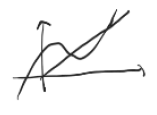
\includegraphics[width=0.3\linewidth]{figures/kein_eindeutiger_fixpunkt}
    \label{fig:kein_eindeutiger_fixpunkt}
\end{figure}




% !TEX root = ./Vorlesungsmitschrift DIFF 2.tex  
\lecture{Mo 27.04. 10:15}{}
\begin{lemma}[Cauchy-Kriterium für gleichmäßige Konvergenz]\label{cauchy_kriterium_gleichmaessige_konvergenz}\hfill
    \begin{eigenschaftenenumerate}
        \item Sei \( (X,d_x)\) metrischer Raum, sei \( (Y,d_Y)\) ein \emph{vollständiger} metrischer Raum. Sei \( f_n\maps X\to Y\) Folge von Funktionen. Dann konvergiert \( f_n\) gegen \( f\) bezüglich
        \begin{align*}
            d_{\sup}(h,g)\definedas \sup_{t\in X} \underbrace {d_{Y}(f(t),g(t))}_{\in \reals } \quad h,g\maps X\to Y
        \end{align*}
        \tiff \tforall \( \varepsilon>0\) \texists \( N=N(\varepsilon)\in \naturals \) \sd
        \begin{align*}
            d_Y(f_n(t),f_m(t))<\varepsilon \quad \forall t\in X\logicspace n,m\geq N(\varepsilon).\tag{\(*\)}\label{eq:cauchy_kriterium_gleichmaessige_konvergenz}
        \end{align*} 
        \begin{notation*}
            Man spricht von \emph{gleichmäßiger Konvergenz}.
        \end{notation*}
        \minisec{Beachte:} Der wesentliche Punkt in \eqref{eq:cauchy_kriterium_gleichmaessige_konvergenz} ist, dass \( N\) unabhängig von \( t\) gewählt werden kann.
        
        \begin{proof}
            Wir stellen zunächst fest, dass \( d_{\sup}\) auf
            \begin{align*}
                \mathcal{F}\definedas \Set{f \maps X\to Y|\text{Für je zwei Funktionen gilt: }d_{\sup}(f_1,f_2)<\infty}
            \end{align*} 
            eine Metrik definiert (auch wenn \( Y\) nicht vollständig ist).
            \begin{proofdescription}
                \item[\ref{metrik:nicht_ausgeartet}] \begin{align*}
                    &d_{\sup}(f,g)=0\\
                    \iff &d_{Y}(f(t),g(t))=0 \logicspace \forall t\in X\\
                    \explain{d_Y\text{ ist Metrik}}{\iff} &f(t)=g(t)\logicspace \forall t\in X
                \end{align*}
                \item[\ref{metrik:symmetrisch}]
                \begin{align*}
                    d_{\sup}(f,g)=\sup d_Y(f(t),g(t))=\sup d_Y(g(t),f(t))=d_{\sup}(g,f)
                \end{align*} 
                \item[\ref{metrik:dreiecksungleichung}] \begin{align*}
                    d_{\sup}(f,g)
                    \begin{aligned}[t]
                        &=\sup \underbrace{d_Y(f(t),g(t))}_{\mathclap{\leq d_Y(f(t),h(t))+d_Y(h(t),g(t))}}\\
                        &\leq \sup d_Y(f(t),h(t))+\sup d_Y(h(t),g(t))\\
                        &=d_{\sup} (f,h)+d_{\sup} (h,g)
                    \end{aligned}
                \end{align*}
            \end{proofdescription}
            \minisec{Zum Beweis der Behauptung:}
            \begin{proofdescription}
                \item[\hin] \begin{align*}
                    \sup_t d_Y(f_n(t),f(t))<\varepsilon\quad \forall n\geq N(\varepsilon)
                \end{align*}
                impliziert
                \begin{align*}
                    d_Y(f_n(t),f(t))<\varepsilon\quad \forall t\in X\logicspace \forall n\geq N(\varepsilon),
                \end{align*} 
                somit für \emph{alle} \( t\in X\)
                \begin{align*}
                    d_Y(f_n(t),f_m(t))\begin{aligned}[t]
                        &\underset{\mathclap{\triangle(d_Y)}}{\leq} d_Y(f_n(t),f(t))+d_Y(f(t),f_m(t))\\
                        &<2\varepsilon \quad \forall n,m\geq N(\varepsilon)
                    \end{aligned}
                \end{align*} 
                \item[\rueck] Gelte \eqref{eq:cauchy_kriterium_gleichmaessige_konvergenz}. Dann ist für jedes \( t\in X\), dass \( (f_n(t))_n\) ist Cauchy-Folge in \( Y\).  
                
                Vollständigkeit von \( Y\) \timplies \( (f_n(t))_n\) konvergiert. Setze \( f(t)\definedas \lim\limits_{n \goesto \infty} f_n(t)\).
                
                Wir zeigen \( f_n\) konvergiert bezüglich \( d_{\sup}\) gegen \( f\). Sei also \( \varepsilon>0\). Wähle in \eqref{eq:cauchy_kriterium_gleichmaessige_konvergenz} \( m\geq N(\varepsilon)\) fest. Dann gilt für \emph{alle} \( t\):
                \begin{align*}
                    \varepsilon \begin{aligned}[t]
                        &\geq \lim\limits_{n \goesto \infty} d_Y(f_n(t),f_m(t))\\
                        &\explain{d_Y\text{ ist stetig}}{=} d_Y(f(t),f_m(t)).
                    \end{aligned}
                \end{align*}
                Das gilt für alle \( m\geq N(\varepsilon)\), \tforall \( t\), also auch für das Supremum \timplies \Beh.
            \end{proofdescription}
            
            
        \end{proof}
        \item \label{gleichmaessige_konvergenz_stetigkeit}Seien \( X,Y\) metrische Räume, \( (f_n)_n\) eine Folge \emph{stetiger} Funktionen \( f_n\maps X\to Y\), die gleichmäßig konvergiere. Dann ist die Grenzfunktion \( f\maps X\to Y\).
        \begin{proof}
            Sei \( a\in X\). Sei \( \varepsilon>0 \). Gleichmäßige Konvergenz \timplies \texists \( N=N(\varepsilon)\in \naturals \) \sd 
            \begin{align*}
                d_Y(f(t),f_n(t))<\varepsilon\quad \forall t\in X\logicspace \forall n\geq N
            \end{align*} 
            \( f_n\) stetig in \( a\) \timplies \texists \( \delta > 0 \) \sd
            \begin{align*}
                &d_Y(d_N(t),f_N(a))<\varepsilon\quad \forall t\text{ mit } d_X(t,a)<\delta\\
                \implies &d_Y(f(t),f(a))\begin{aligned}[t]
                    &\underset{\triangle}{\leq}d_Y(f(t),f_N(t))+d_Y(f_N(t),f_N(a))+d_Y(f_N(a),f(a))\\
                    &<3\varepsilon\quad \forall t\text{ mit }d_X(t,a)<\delta.
                \end{aligned}
            \end{align*}
            
        \end{proof}
         
    \end{eigenschaftenenumerate}
        
\end{lemma}
\begin{folgerung*}
    \begin{align*}
        (C(\explain{\text{Stellt man diese Bedingung, ist automatisch garantiert, dass \( d_{\sup}(f_1,f_2)=\sup_{t\in \rinterval{a}{b}}\abs{f_1(t)-f_2(t)}<\infty \)}}{\interval{a}{b}},\reals),d_{\sup})
    \end{align*}, \( D\subset \reals \), ist vollständig.  
\end{folgerung*}
\begin{proof}
    Sei \( (f_n)_n\) Cauchy-Folge in \( C(D,\reals )\) bezüglich \( d_{\sup}\), \dh zu \( \varepsilon>0 \) \texists \( N=N(\varepsilon)\) \sd
    \begin{align*}
        &d_{\sup}(f_n,f_m)<\varepsilon\quad \forall n,m\geq N(\varepsilon)\\
        \implies &d_Y(f_n(t),f_m(t))=\abs{f_n(t)-f_m(t)}<\varepsilon \quad \forall n,m\geq N(\varepsilon)\logicspace \forall t\in D. 
    \end{align*} 
    \( \reals \) ist vollständig
    \begin{proofdescription}
        \item[\( \overset{\text{\ref{cauchy_kriterium_gleichmaessige_konvergenz}}}{\implies}\)] \( (f_n)_n\) konvergiert bezüglich \( d_{\sup}\) gegen seinen punktweisen Grenzwert
        \begin{align*}
            f(t)\definedas \lim\limits_{n \goesto \infty} f_n(t)\quad (\text{Konvergenz in \( \reals \)})
        \end{align*}   
        \item[\( \overset{\text{\ref{gleichmaessige_konvergenz_stetigkeit}}}{\implies}\)] \( t\mapsto f(t)\) ist stetig. 
    \end{proofdescription}
    
\end{proof}
\section*{Stetige Abbildungen auf metrischen Räumen}
\begin{lemma}\label{metrische_raeume_komposition_stetig}
    Seien \( X,Y,Z\) metrische Räume, \( f\maps X\to Y\), \( g\maps Y\to Z\), \( f(X)\subset Y\). Ist \( f\) stetig in \( a\in X\) und \( g\) stetig in \( b=f(a)\in \tilde{Y} \), so ist \( g\circ f\maps X\to Z\) stetig in \( a\).
\end{lemma}
\begin{proof} (Über Folgenstetigkeit, \thref{stetigkeit:folgenkonvergenzkriterium})
    Sei \( x_n\goesto a\) \timplies \( \lim f(x_n)=(a)=b\) und \( \lim g(f(x_n))=g(b)=g(f(a))\) \timplies \( \lim g\circ f(x_n)=g\circ f(a)\).   
    
\end{proof}
\begin{definition}
    Auf dem \( \reals^n\) ist durch
    \begin{align*}
        d_{\max}(x,y)\definedas \max_{i\in \Set{1,\ldots,n}}\abs{x_i-y_i}. 
    \end{align*}
    eine Metrik definiert.
\end{definition}
\begin{bemerkungen*}
    \begin{enumerate}
        \item \( d_{\max}(x,y)=d_{\sup}(x,y)\), fasst man \( x\) und \( y\) als Abbildungen
        \begin{align*}
            x\maps \Set{1,\ldots, n}\to \reals 
        \end{align*} 
        auf, \( x(i)=x_i\).
        \item \label{d_max:folgenkonvergenz}Eine Folge \( (x_m)_m\subset \reals^n \), \( x_m=(x_m^1,\ldots, x_m^n)\) konvergiert bezüglich \( d_{\max}\) \tiff Alle \emph{Komponentenfolgen} \( (x_m^i)_m\quad (1\leq i\leq n)\) konvergieren in \( \reals \).
        \begin{proof}
            \begin{proofdescription}
                \item[\hin] Zu \( \varepsilon>0\) \texists \( N\) \sd \( \max \abs{x_m^i-a_m^i}<\varepsilon\quad \forall m\geq N \).
                \item[\rueck] Zu \( \varepsilon>0\) \texists \( N_i\) \sd \( \abs{x_m^i-a_m^i}<\varepsilon \quad \forall m\geq N_i\)
                \begin{align*}
                    \implies \max_i \abs{x_m^i-a_m^i}<\varepsilon\quad \forall m\geq N=\max\Set{N_1,\ldots, N_n}. 
                \end{align*} 
            \end{proofdescription}
            
            
        \end{proof}
        
        \item Es folgt: \( (\reals^n, d_{\max})\) ist \emph{vollständig}.
        \item \( B_\varepsilon(a)\) bezüglich dieser Metrik:
        \begin{align*}
            \Set{x\in \reals ^n |\max_{i\in \Set{1,\ldots, n}}\abs{x_i-a_i}<\varepsilon},
        \end{align*}
        Würfel mit Seitenlängen \( 2\varepsilon\) um \( a\).
        \begin{figure}[H]
            \centering
            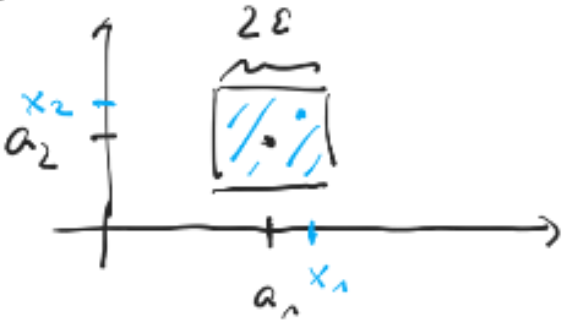
\includegraphics[width=0.3\linewidth]{figures/d_max_ball}
            \label{fig:d_max_ball}
        \end{figure}
        
    \end{enumerate}
\end{bemerkungen*}

\begin{lemma}\label{d_max:metrischer_raum_zu_r_stetigkeit:komponenten}
    Sei \( (X,d)\) metrischer Raum. Sei \( @rr
    ^n\) mit \( d_{\max}\) versehen. Eine Abbildung \( f\maps X\to \reals ^n\), \( f=(f_1,\ldots, f_n)^T\), 
    \begin{align*}
        f(y)=(f_1(y),\ldots, f_n(y))^T\in \reals^n, y\in X.
    \end{align*}   
    \( f_i\maps X\to \reals \), \( i\in \Set{1,\ldots,n}\), \enquote{\emph{Komponenten-Funktionen}}, ist genau dann stetig in \( a\in X\), falls alle \( f_i\) stetig in \( a\) sind.
\end{lemma}
\begin{proof}
    Mit Folgenstetigkeit direkt aus Bemerkung~\ref{d_max:folgenkonvergenz}. Hier nochmals mit \( \varepsilon\)-\( \delta\)-Kriterium.
    \begin{notation*}
        \( \underline{n}=\Set{1,\ldots,n}\). 
    \end{notation*}
    \begin{proofdescription}
        \item[\hin] Sei also \( f\maps X\to \reals^n\) stetig in \( a\). Sei \( \varepsilon>0\). Dann \texists \( \delta>0\) \sd
        \begin{align*}
            &\max_{i\in \underline{n}}\abs{f_i(y)-f_i(a)}<\varepsilon\forall y\in \explain{\text{bezüglich }d}{B_\delta(a)}\\
            \implies &\abs{f_i(y)-f_i(a)}<\varepsilon\quad \forall y\in B_\delta(a)\logicspace \forall i\in \underline{n}\\
            \implies &f_i\text{ sind stetig in }a.
        \end{align*}  
        \item[\rueck] Seien also die \( f_i\maps X\to \reals \), \( i\in \underline{n}\), stetig in \( a\). Sei \( \varepsilon>0\). Dann \texists \( \delta_i>0\) \sd 
        \begin{align*}
            \abs{f_i(y)-f_y(a)}<\varepsilon\quad \forall y\in B_{d_i}(a)\subset X. 
        \end{align*}   
        Wähle \( d\definedas \min \Set{\delta_1,\ldots,\delta_n}\). Dann ist
        \begin{align*}
            \max_{i\in \underline{n}}\abs{f_i(y)-f_i(a)}<\varepsilon\quad \forall y\in B_d(a). 
        \end{align*} 
    \end{proofdescription}
\end{proof}
\begin{lemma}\label{d_max:operationen_stetig}
    Folgende Abbildungen sind stetig:
    \begin{align*}
        \operatorname{add}\maps \reals^2\to \reals,\logicspace \operatorname{add}(x,y)=x+y\\
        \operatorname{mult}\maps \reals^2\to \reals,\logicspace \operatorname{mult}(x,y)=x\cdot y\\
        \operatorname{quot}\maps \reals \times\equalto{\reals \setminus\zeroset}{\reals^{*}}\to \reals,\logicspace \operatorname{quot}(x,y)=x/y.
    \end{align*}
    Hierbei sei \( \reals^2\), \( \reals \times\reals^{*}\), mit \( d_{\max}\) versehen.
\end{lemma}
\begin{proof}
    Sei \( ((x_m,y_m))_m\subset \reals^2\) mit \( (x_m,y_m)\goesto (x,y)\) (bezüglich \( d_{\max}\))
    \begin{align*}
        \underset{\text{Bem~\ref{d_max:folgenkonvergenz}}}{\implies} &x_m\goesto x\text{ und }x_m\goesto y\text{ in }\reals \\
        \implies& \lim (x_m+y_m)=x+y\\
        &\lim (x_m\cdot y_m)=x\cdot y\\
        &\lim (x_m/y_m)=x/y\quad (\text{falls }y_m \neq 0,y\neq 0).
    \end{align*}
    
\end{proof}
\begin{folgerung*}
    Sei \( (X,d)\) metrischer Raum. Seien \( f,g\maps X\to \reals \) stetig. Dann sind auch
    \begin{align*}
        f+g&\maps X\to \reals,\logicspace  (f+g)(x)=f(x)+g(x) \text{ und}\\
        g\cdot g&\maps X\to \reals,\logicspace (f\cdot g)(x)=f(x)\cdot g(x)
    \end{align*}
    stetig. Gilt \( g(x)\neq 0 \quad \forall x\in X\), so ist auch
    \begin{align*}
        f/g\maps X\to \reals, (f/g)(x)=f(x)/g(x)
    \end{align*}
    stetig.
\end{folgerung*}
\begin{proof}
    \begin{align*}
        \ref{d_max:metrischer_raum_zu_r_stetigkeit:komponenten} \implies \begin{pNiceMatrix} f \\ g \end{pNiceMatrix}\maps X\to \reals^2, \begin{pNiceMatrix} f \\ g \end{pNiceMatrix}(x)=\begin{pNiceMatrix} f(x) \\ g(x) \end{pNiceMatrix}  
    \end{align*}
    ist stetig. 

    Es ist
    \begin{align*}
        f+g&=\operatorname{add}\circ \begin{pNiceMatrix} f \\ g \end{pNiceMatrix}\\
        f+g&=\operatorname{mult}\circ \begin{pNiceMatrix} f \\ g \end{pNiceMatrix}\\
        f/g&=\operatorname{quot}\circ \begin{pNiceMatrix} f \\ g \end{pNiceMatrix}
    \end{align*}
    Mit \ref{d_max:operationen_stetig} und \ref{metrische_raeume_komposition_stetig} folgt die Behauptung.
\end{proof}
\begin{beispiel*}
    Polynomische Funktionen \( \reals^n\to \reals \) 
    \begin{align*}
        x\mapsto \sum\limits_{0\leq k_i\leq r}c_{\underbrace{k_1\cdots k_n}_{\in \reals}}x_1^{k_1}\cdots x_n^{k_n} 
    \end{align*}
    sind stetig.
\end{beispiel*}
\begin{bemerkung}
    Wir werden später sehen, dass die Aussage in \ref{d_max:operationen_stetig} auch gilt, wenn man den \( \reals ^2\) \zb mit dem Euklidischen Abstand versieht.
\end{bemerkung}
\section*{Kompaktheit}
\begin{definition}
    Sei \( (X,d)\) metrischer Raum, \( M\subset X\). Eine \emph{offene Überdeckung von \( M\)} ist eine Familie \( (U_i)_{i\in I}\) von offenen Teilmengen \( U_i\subset X\) mit \( M\subset \bigcup\limits_{i\in I}U_i\) (\( I\) eine beliebige Indexmenge).   
\end{definition}
\begin{definition}
    \( M\subset X\) heißt \emph{kompakt}, falls es zu \emph{jeder} offenen Überdeckung von \( \bigcup_{i\in I} U_i \) von \( M\) \emph{endlich} viele Indizes \( i_1,\ldots, i_N\) gibt \sd
    \begin{align*}
        M\subset U_{i_1}\cup \cdots \cup U_{i_N}.
    \end{align*} 

    \begin{achtung*}
        Ein nicht-kompakter raum kann eine endliche Überdeckung \( U_1\cup \cdots \cup U_N\) besitzen. Die Aussage der Definition ist, dass man aus \emph{jeder} offenen Überdeckung endlich viele offene Mengen wählen kann, die \( M\) noch ganz überdecken!
    \end{achtung*}
\end{definition}
\begin{beispiele}
    \begin{enumerate}
        \item \( \interval{a}{b} \) ist kompakt (Beweis später).
        \item \( \ointerval{a}{b} \) ist nicht kompakt (obwohl etwa \( \ointerval{a}{b} \) eine endliche offene Überdeckung ist!)
        \begin{proof}
            \begin{align*}
                U_j=\ointerval{a+\frac{1}{j}}{b},\logicspace j\geq 1\\
                \bigcup_j U_j=\ointerval{a}{b} 
            \end{align*}
            aber ed gibt \emph{kein} \( N\) \sd
                \( \bigcup\limits_{j=1}^{N}U_j\supset \ointerval{a}{b} \), denn \zb \( a+\frac{1}{N+1}\notin \bigcup_{p=1}^{N}U_j \).  
        \end{proof}
        
        \item Sei \( (x_n)_n\subset X\) gegen \( a\) konvergente Folge. Dann ist \( M=\Set{x_n|n\in \naturals }\cup \Set{a}\) kompakt.
        \begin{proof}
            Sei \( (U_j)_j\) eine offene Überdeckung von \( M\)
            \begin{align*}
                a\in M\implies \exists j_0\logicspace\text{\sd} \logicspace a\in U_{j_0}
            \end{align*} 
            \( U_{j_0}\) ist offen, also eine Umgebung von \( a\).
            \begin{align*}
                \implies \exists N\logicspace\text{\sd} \logicspace  x_n\in U_{j_0}\quad \forall n\geq N.
            \end{align*}
        \end{proof}
        
        \item Sei \( (X_i,d_{\text{discrete}})\). Dann sind genau die endlichen Mengen kompakt.
        \begin{proof}
            Betrachte \( \bigcup_{x\in M} \Set{x}\). 
        \end{proof}        
    \end{enumerate}
\end{beispiele}
\begin{satz}\label{kompakt:abgeschlossen_beschraenkt}
    Sei \( (X,d)\) metrischer Raum, \( K\subset X\) kompakt. Dann ist \( K\) abgeschlossen und beschränkt. 
\end{satz}
\begin{proof}
    \begin{proofdescription}
        \item[Abgeschlossen:] Sei \( a\in X\setminus K\). Setze zu \( n\geq 1\)
        \begin{align*}
            U_n\definedas \Set{y\in X| d(y,a)>\frac{1}{n}}
        \end{align*}  
        \begin{figure}[H]
            \centering
            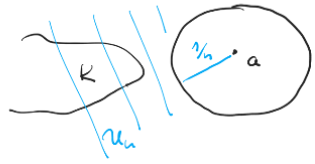
\includegraphics[width=0.5\linewidth]{figures/kompakt_abgeschlossen_beweis}
            \label{fig:kompakt_abgeschlossen_beweis}
        \end{figure}
        \( U_n\) ist offen (denn \( X\setminus U_n=\overline{B_{1/n}(a)}\)) und \( \bigcup_{n=1}^{\infty}U_n=X\setminus \Set{a}\supset K\).
        \( K\) kompakt \timplies \texists \( U_{n_1},\ldots, U_{n_L}\) \sd \( K\subset U_{n_1}\cup \cdots \cup U_{n_l}\). Setze \( N\definedas \max\Set{n_1,\ldots,n_l}\). Dann ist \( B_{\frac{1}{N}}(a)\subset X\setminus K\) \timplies \( X\setminus K \) ist offen \timplies \Beh.
        
        \item[Beschränktheit:] Sei \( a\in X\). Dann ist \( X=\bigcup\limits_{n=1}^{\infty} B_n(a) \) und somit \( (B_n(a))_n\) eine offene Überdeckung von \( K\).
        \begin{align*}
            \implies &\exists n_1,\ldots, n_k\logicspace\text{\sd}\logicspace  K\subset B_{n_1(a)}\cup \cdots B_{n_k}(a)\\
            \implies &K\subset B_N(a) \text{ für }N=\max\Set{n_1,\ldots,n_k}\\
            \implies &\diam(K)\leq 2N.
        \end{align*}     
    \end{proofdescription}    
\end{proof}
\begin{folgerung*}
    Konvergente Folgen sind beschränkt.
\end{folgerung*}
\begin{bemerkung*}
    Die Umkehrung von \ref{kompakt:abgeschlossen_beschraenkt} gilt im Allgemeinen nicht!
    
    \( (X,d_{\text{discrete}})\), \( X\) habe unendlich viele Elemente. Jede Teilmenge ist abgeschlossen (da jede offen ist) und beschränkt (durch \( 1\)), aber nur die \emph{endlichen} sind kompakt.
\end{bemerkung*}
\begin{lemma}\label{abgeschlossene_teilmenge_kompakter_menge_ist_kompakt}
    Ist \( K\subset X\) kompakt und \( A\subset K\) ist abgeschlossen, so ist \( A\) kompakt.
\end{lemma}
\begin{proof}
    Sei \( (U_j)_j\) offene Überdeckung von \( A\). Es ist
    \begin{align*}
        &(\underbrace{X\setminus A}_{\mathclap{\text{offen (VOR)}}})\cup \bigcup U_j=X\supset K\\
        \implies &\exists j_1,\ldots, j_L\logicspace\text{\sd}\logicspace K\subset (X\setminus A)\cup U_{j_1}\cup \cdots \cup U_{j_L}\\
        \implies &A\subset U_{j_1}\cup \cdots \cup U_{j_L}.  
    \end{align*}
    
\end{proof}


\begin{satz}\label{kompakte_menge_stetiges_bild_kompakt}
    Seien \( X,Y\) metrische Räume und \( f\maps X\to Y\) stetig. Ist \( K\subset X\) kompakt, so ist auch \( f(K)\subset Y\) kompakt. 
\end{satz}
\begin{proof}
    Sei \( (U_j)_j\) offene Überdeckung von \( f(K)\). \( f\) stetig \( \underset{\ref{stetigkeit_in_topologischen_raeumen:urbildkriterium}}{\implies}\) Die Urbilder \( V_j \definedas \inv{f}(U_j)\) sind offen.
    
    Und nach Definition ist \( K\subset \bigcup_j V_j\).
    \begin{align*}
        \underset{\text{VOR}}{\implies} \exists j_1,\ldots, j_N\logicspace \text{\sd}\logicspace  K\subset V_{j_1}\cup \cdots \cup V_{j_N}\\
        \implies f(K)\subset U_{j_1}\cup \cdots\cup U_{j_N}.
    \end{align*} 
    
\end{proof}

\begin{satz}\label{funktion_von_kompaktem_metrischen_raum_zu_r_kriegt_min_max}
    Sei \( \mathfrak{X}\) kompakter metrischer Raum, \( f\maps \mathfrak{X}\to \reals \) stetig. Dann ist \( f\) beschränkt und nimmt ihr Maximum und Minimum an, \dh \texists \( a,b \in \mathfrak{X}\)
    \begin{align*}
        f(a)=\sup\Set{f(x)|x\in \mathfrak{X}},\quad f(b)=\inf\Set{f(x)|x\in \mathfrak{X}}.
    \end{align*} 
\end{satz}
\begin{proof}
    \ref{kompakte_menge_stetiges_bild_kompakt} \timplies \( f(\mathfrak{X})\) ist kompakt. Mit \ref{kompakt:abgeschlossen_beschraenkt} folgt: \( f(\mathfrak{X})\) ist beschränkt (somit ist \( f\) beschränkt) und abgeschlossen.
    
    Also sind \( \sup f(\mathfrak{X})\) und \( \inf(\mathfrak{X})\) endlich. Zudem gibt es
    \begin{align*}
        (y_k)_k &\subset f(\mathfrak{X}),\quad y_k\goesto \sup(f(\mathfrak{X}))\\
        (z_k)_k\subset f(\mathfrak{X}), \quad z_k\goesto \inf(\mathfrak{X}),
    \end{align*}
    somit (Abgeschlossenheit!)
    \begin{align*}
        \sup(f(\mathfrak{X}))\in f(\mathfrak{X})\\
        \inf(f(\mathfrak{X}))\in f(\mathfrak{X})
    \end{align*}
    \timplies \Beh.
\end{proof}

\begin{beispiel*}
    Sei \( (\mathfrak{X},d)\) metrischer Raum. \( M\subset \mathfrak{X}\). Sei \( x\in \mathfrak{X}\). Der \emph{Abstand} von \( a\) zu \( M\) ist definiert als
    \begin{align*}
        \dist(x,M)\definedas \inf\Set{d(x,y)|y\in M}.
    \end{align*} 
    \begin{behauptung*}
        \( x\mapsto \dist(x,M)\) ist stetig auf \( \mathfrak{X}\). 
    \end{behauptung*}
    \begin{proof}
        Sei \( \varepsilon>0\). Dann ist
        \begin{align*}
            \abs{\dist(x,M)-\dist(\tilde{x},M)}\leq d(x,\tilde{x})<\varepsilon \quad \text{falls }d(x,\tilde{x})<\varepsilon, 
        \end{align*}
        denn
        \begin{align*}
            \dist(x,M)\underset{\triangle}{\leq}d(x,\tilde{x})+\dist(\tilde{x},M)\quad \forall x,\tilde{x}\in \mathfrak{X}.
        \end{align*}
        
    \end{proof}
    Definiere zu \( K\subset \mathfrak{X} \)
    \begin{align*}
        \dist(K,M)\definedas \inf\Set{\dist(x,M)|x\in K}.
    \end{align*}
    \begin{behauptung*}
        Ist \( M \) abgeschlossen, \( K \) kompakt und ist \( M\cap K=\emptyset \), so gilt \( \dist(M,K)>0 \).
    \end{behauptung*}
    \begin{proof}
        \( x\mapsto \dist(x,M) \) ist stetig auf \( \mathfrak{X} \), somit erst recht auf \( K \). \( K \) ist kompakt \( \overset{\ref{funktion_von_kompaktem_metrischen_raum_zu_r_kriegt_min_max}}{\implies} \) \texists \( a\in K \) \sd \( \dist(a,M)=\dist(K,M) \). \( M \) abgeschlossen \timplies \texists \( \varepsilon>0 \) \sd \( B_{\varepsilon}(a)\subset X\setminus K \) \timplies \( \dist(a,M)\geq \varepsilon \).
        
    \end{proof}
    \begin{achtung*}
        \begin{enumerate}
            \item Betrachte
            \begin{align*}
                M=\Set{(x,y)|xy=0}\subset , N=\set{(x,y)|xy=1}\subset \reals^2\\
                \dist(M,N)=0.
            \end{align*}
            \begin{figure}[H]
                \centering
                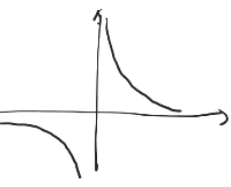
\includegraphics[width=0.3\linewidth]{figures/achsen_und_eins_durch_x}
                \caption*{}
                \label{fig:achsen_und_eins_durch_x}
            \end{figure}
            
            \item Betrachte \( B_{1/2}(1) \), \( B_{1/2}(2)\subset \reals^2 \), \( d_{\text{Euklidisch}} \). Distanz ist \( 0 \).
            \begin{figure}[H]
                \centering
                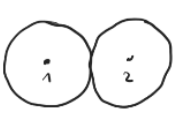
\includegraphics[width=0.3\linewidth]{figures/beruehrende_kreise}
                \label{fig:beruehrende_kreise}
            \end{figure}
            
        \end{enumerate}
    \end{achtung*}    
\end{beispiel*}
\begin{satzdef}
    Seien \( \mathfrak{X},Y \) metrische Räume, \( \mathfrak{X} \) kompakt. Dann ist jede stetig Abbildung \( f\maps \mathfrak{X}\to Y \) sogar \emph{gleichmäßig stetig} \dh im \( \varepsilon \)-\( \delta \)-Kriterium kann \( \delta \) unabhängig von \( x \) gewählt werden:
    \begin{align*}
        \forall \varepsilon>0\logicspace \exists \delta>0\logicspace\text{\sd}\logicspace d_Y(f(x),f(\tilde{x}))<\varepsilon\quad \forall x,\tilde{x},d_{\mathfrak{X}}(x,\tilde{x})<\delta.
    \end{align*}
\end{satzdef}
\begin{proof}
    Sei \( \varepsilon>0 \). Dann gibt es zu \( a\in \mathfrak{X} \) ein \( \delta(a)>0 \) \sd
    \begin{align*}
        d_Y(f(a),f(y))<\varepsilon\quad \forall y\in B_{\delta(a)}(a).
    \end{align*}
    Es gilt \( \bigcup_{a\in X} B_{\frac{\delta(a)}{2}}(a)=\mathfrak{X}\).

    \( \mathfrak{X} \) ist kompakt \timplies \texists \( a_1,\ldots,a_N \) \sd \( X=\bigcup\limits_{j=1}^{N}B_{\delta(a_j)/2} (a_j)\). Setze 
    \begin{align*}
        \delta\definedas \frac{1}{2}\min\Set{\delta(a_1),\ldots,\delta(a_N)}.
    \end{align*}

    Seien jetzt \( x,\tilde{x} \) beliebig aus \( \mathfrak{X} \) mit \( d_{\mathfrak{X}}(x,\tilde{x})<\delta \). Dann gibt es ein \( j\in \Set{1,\ldots, N} \) \sd \( x\in B_{\delta(a_j)/2} \) und somit \( \tilde{x}\in B_{\delta(a_j)}(a_j) \)
    \begin{align*}
        \implies &d_Y(f(x),f(a_j))<\varepsilon \quad d_Y(f(\tilde{x}),f(a_j))<\varepsilon\\
        \implies &d_Y(f(x),f(\tilde{x}))<2\varepsilon \quad \forall x,\tilde{x},\logicspace d_{\mathfrak{X}}(x,\tilde{x})<\delta.
    \end{align*}
    \begin{figure}[H]
        \centering
        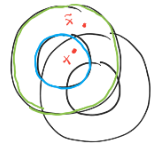
\includegraphics[width=0.4\linewidth]{figures/doppel_doppel_ball}
        \label{fig:doppel_doppel_ball}
    \end{figure}
    
\end{proof}
\begin{satz}[Bolzano-Weierstraß]\label{bolzanoweierstrass}
    Sei \( (X,d) \) metrischer Raum. Sei \( K\subset X \) kompakt. Dann besitzt jede Folge \( (x_n)_n \) in \( K \) eine Teilfolge \( (x_{n_k})_k \), die gegen einen Punkt \( x\in K \) konvergiert. 
\end{satz}
\begin{proof}
    Angenommen, \tnexists Teilfolge, die gegen einen Punkt von \( K \) konvergiert. Dann besitzt jedes \( x\in K \) eine offene Umgebung \( U_x \), in der nur endlich viele Folgenglieder liegen (sonst könnte man eine gegen \( x \) konvergente Teilfolge konstruieren). Es gilt: \( \bigcup_{x\in K}U_x\supset K \)
    \begin{align*}
        \implies \exists x_1,\ldots, x_N\logicspace\text{\sd} \logicspace \bigcup_{j=1}^{N}U_{x_j}\subset K   
    \end{align*}
    Aber dann liegen nur endlich viele \( x_k \) in \( K \), \contra zur Definition.
    
\end{proof}




% !TEX root = ./Vorlesungsmitschrift DIFF 2.tex  
\lecture{Do 30.04. 10:15}{}
\section{Äquivalenz von Metriken}
Wir haben gesehen, dass die Eigenschaften derselben Menge sehr verschieden sein können, je nachdem mit welcher Topologie man sie versieht.
\begin{beispiel*}
    \( \reals \) mit der Standardtopologie \( \abs{x-y} \):
    \begin{itemize}
        \item \( \linterval{a}{b} \) ist nicht offen, \( \interval{a}{b} \) ist kompakt.
    \end{itemize}
    \( \reals \) mit der diskreten Metrik \( d_{\text{disk}} \)
    \begin{itemize}
        \item Alle Teilmengen sind offen.
        \item Nur endliche Teilmengen sind kompakt.
        \item Konvergiert \( x_n\goesto a \) (bezüglich \( d_{\text{disk}} \)),so muss gelten \( \exists N \) \sd \( x_n=a\quad \forall n\geq N \) (denn \( \Set{a} \) ist Umgebung von \( a \), oder anders gesagt: damit \( \distance{x_n}{a}<\varepsilon<1 \) wird, muss gelten \( x_n=a \)).
        \item \emph{Alle} Abbildungen \( f\maps (X,d_{\text{disc}})\to (Y,d) \) sind stetig. (Beweis am einfachsten über Folgenstetigkeit).
    \end{itemize}
    Andererseits gilt:\\
    \( U\subset \reals^2 \) ist offen in \( (\reals^2,d_{\text{Eukl}}) \) \tiff \( U \) ist offen in \( (\reals^2, d_{\max}) \).
    \begin{proof}
        \begin{proofdescription}
            \item[\hin] Sei \( a\in U \) \( \overset{VOR}{\implies} \) \texists \( \varepsilon>0 \) \sd
            \begin{align*}
                \ball;{\varepsilon}^{d_\text{E}}(a)\definedas \Set{x\in \reals^2|d_{\text{Eukl}(x,a)}=\sqrt{(x_1-a_1)^2+(x_2-a_2)^2}<\varepsilon}\subset U
            \end{align*} 
        \end{proofdescription}
        Da \( \ball;{\rho}^{d_{\max}}(a)\subset \ball;{\varepsilon}^{d_{\text{E}}}(a) \) für \( \rho=\frac{\varepsilon}{\sqrt{2}} \), ist \( U \) auch offen \( (\reals^2, d_{\max}) \).
        \begin{figure}[H]
            \centering
            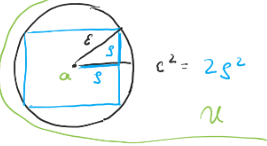
\includegraphics[width=0.5\linewidth]{figures/max_quadrat_in_eukl_kreis}
            \label{fig:max_quadrat_in_eukl_kreis}
        \end{figure}
        \item[\rueck] Sei \( a\in U \)\( \overset{VOR}{\implies} \)\texists \( \varepsilon>0 \) \sd
        \begin{align*}
            \ball;{\varepsilon}^{d_{\max}}(a)=\Set{x|d_{\max}(x,a)<\varepsilon}\subset U.
        \end{align*}
        Es gilt \( \ball;{\rho}^{d_{\text{E}}}(a)\subset \ball;{\varepsilon}^{d_{\max}}(a) \) für \( \rho=\varepsilon \), also ist \( U \) offen in \( (\reals^2,d_{\text{Eukl}}) \).
        \begin{figure}[H]
            \centering
            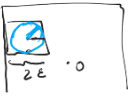
\includegraphics[width=0.4\linewidth]{figures/eukl_kreis_in_max_quadrat}
            \label{fig:eukl_kreis_in_max_quadrat}
        \end{figure}
        
    \end{proof}
    
\end{beispiel*}
\begin{definition}\index{Stärke von Metriken}
    Sei \( X \) eine Menge, seien \( d \) und \( \tilde{d} \) Metriken auf \( X \). Dann nennt man \( d \) \emph{stärker} (feiner) als \( \tilde{d} \), falls jede bezüglich \( \tilde{d} \) offene Menge auch offen bezüglich \( d \) ist, und \emph{schwächer} (gröber), falls \( \tilde{d} \) stärker ist als \( d \). Ist \( d \) sowohl stärker als auch schwächer als \( \tilde{d} \), so nennt man \( d \) und \( \tilde{d} \) \emph{äquivalent}.
\end{definition}
\begin{beispiel*}
    \( d_{\max} \) ist äquivalent zu \( d_{\text{Eukl}} \). \( d_{\text{disk}} \) ist stärker als \( d_{\max}  \) und nicht schwächer.
\end{beispiel*}
\begin{bemerkungen}
    Sei \( d \) stärker als \( \tilde{d} \). Dann gilt:
    \begin{enumerate}
        \item Konvergiert eine Folge bezüglich der stärkeren Metrik, so auch bezüglich der schwächeren.
        
        (denn: Konvergiere \( x_n\to a \) (bezüglich \( d \)). Sei \( \varepsilon>0 \). Betrachte \( \ball;{\varepsilon}^{\tilde{d}}(a)=U \) offen bezüglich \( d \) \timplies \( U \) Umgebung von \( a \) (bezüglich \( d \)) \timplies \( U \) Umgebung von \( a \) (bezüglich \( d \)) \timplies \texists  \( N \) \sd \( x_n\in U\quad \forall n\geq N \).)
        
        \item Ist eine Funktion \( f\maps (X,\tilde{d})\to (Y,d_Y) \) stetig, so auch \( f\maps (X,d)\to (Y,d_Y) \).
        \item Ist eine Funktion \( f\maps (Y,d_Y)\to (X,d) \) stetig, so auch \( f\maps (Y,d_Y)\to (X,\tilde{d}) \).
        
        \begin{proof}
            \( f \) stetig \tiff Urbilder offener Mengen sind offen.
            \begin{proofenumerate}
                \stepcounter{enumi}
                \item \( U\subset Y \) \timplies \( \inverse{f}(U) \) offen bezüglich \( \tilde{d} \) \timplies \( \inverse{f}(U) \) offen bezüglich \( d \).
                \item Sei \( U\subset X \) offen bezüglich \( \tilde{d} \), also auch offen bezüglich \( d \) \timplies \( \inverse{f}(U) \) offen in \( Y \).
            \end{proofenumerate}
            
        \end{proof}
        
    \end{enumerate}
\end{bemerkungen}
\begin{bemerkung*}
    Sind \( d \) und \( \tilde{d} \) äquivalent, sind die selben Folgen konvergent, die selben Mengen offen, kompakt, die selben Funktionen stetig etc.
\end{bemerkung*}
\chapter{Normierte Vektorräume}
\begin{definition}\label{norm}\index{Norm}
    Sei \( V \) ein reeller Vektorraum. Eine \emph{Norm} auf \( V \) ist eine Abbildung \( \norm{\cdot}\maps V\to \reals \) mit
    \begin{eigenschaftenenumerate}
        \item\label{norm:positiv_definit}
        \begin{align*}
            \norm{x}=0\iff x=0
        \end{align*}
        \item \label{norm:betrags_homogen}
        \begin{align*}
            \norm{\lambda x}=\abs{\lambda}\norm{x}\quad \forall \lambda\in \rho,\logicspace x\in V
        \end{align*}
        
        \item \label{norm:dreiecksungleichung}\begin{align*}
            \norm{x+y}\leq \norm{x}+\norm{y}\quad \forall x,y\in V
        \end{align*}
        Dreiecksungleichung.
    \end{eigenschaftenenumerate}
    Ein \emph{normierter VR} \( (V,\norm{\cdot}) \) ist ein VR mit einer Norm.
\end{definition}
\begin{beispiele*}
    \begin{itemize}
        \item \( \reals^n \) mit \( \euclidiannorm{\cdot} \) Euklidische Norm auf \( \reals^n \)
        \begin{align*}
            \norm{x}=\sqrt{\sum_{i=1}^{n}x_i^2}\quad x=(x_{1},\dotsc,x_n).
        \end{align*}
        \item \( \reals^n \) mit \( \supnorm{\cdot}=\explicitnorm{\max}{\cdot} \),
        \begin{align*}
            \supnorm{x}=\Max{\Set{\abs{x_1},\dotsc,\abs{x_n}}}.
        \end{align*}
        \item \( \reals^n \) mit \( \norm{\cdot}_p \) \enquote{\( p \)-Norm}, \( p\geq 1 \), \( p\in \reals \).
        \begin{align*}
            \norm{x}_{p}=\p*{ \sum_{i=1}^{n}\abs{x_i}^p }^{1/p}\quad \to\logicspace  \text{Saalübung}.
        \end{align*}
        \item \( \stetigefunktionen(\interval{a}{b}) \) mit \( \norm{f}_{L^1}=\Integrate{\abs{f(t)}}{t,a,b} \). 
        \item \( \stetigefunktionen(\interval{a}{b}) \) mit \( \supnorm{f}=\sup_{t\in \interval{a}{b}}\abs{f(t)} \). 
    \end{itemize}
\end{beispiele*}
\begin{lemma}
    Sei \( (V,\norm{\cdot}) \) normierter VR\@. Dann wird durch \( \distance{x}{y}\definedas \norm{x-y} \) eine Metrik auf \( V \) definiert (\enquote{induziert}).
\end{lemma}
\begin{proof}
    \ref{norm:positiv_definit} (Norm) \timplies \ref{metrik:nicht_ausgeartet} (Metrik). \ref{metrik:symmetrisch} (Symmetrie der Metrik): folgt aus \( \norm{x-y}=\norm{y-x} \).
\end{proof}
\begin{notation*}
    Wir schreiben \( (V,\norm{\cdot}) \) für den \emph{metrischen} Raum, dessen Metrik von \( \norm{\cdot} \) induziert wird.
\end{notation*}
\begin{bemerkung*}
    Nicht jede Metrik auf einem Vektorraum wird von einer Norm induziert, denn induzierte Metriken erfüllen \( \distance{\lambda x}{\lambda y}=\abs{\lambda}\distance{x}{y} \). Die diskrete Metrik erfüllt das nicht.
\end{bemerkung*}
\begin{lemma}\label{normen_staerke_abschaetzung}
    Seien \( d_1 \) und \( d_2 \) auf \( V \) von Normen \( \norm{\cdot}_1 \) und \( \norm{\cdot}_2 \) induziert. Dann ist \( d_2 \) stärker als \( d_1 \) genau dann, wenn es eine positive Zahl \( C>0 \) gibt \sd
    \begin{align*}
        \norm{x}_1\leq C\norm{x}_2\quad \forall x\in V.
    \end{align*}
\end{lemma}
\begin{proof}
    Bezeichne \( \ball;{r}^j(0) \), \( r>0 \), die offenen Kugeln bezüglich \( d_j \).
    \begin{description}
        \item[\hin] Nach VOR ist insbesondere \( B_1^1(0) \) offen bezüglich \( d_2 \) \timplies \texists \( \varepsilon>0 \) \sd \( B_\varepsilon^2(0)\subset B_1^1(0) \) \timplies für \( x\in X \), \( x\neq 0 \) gilt
        \begin{align*}
            &\norm{\frac{\varepsilon x}{2\norm{x}}_2}_2=\frac{\varepsilon}{2}<\varepsilon\\\
            \implies &\norm{\frac{\varepsilon x}{2\norm{x}_2}}_1 <1 \\
            \implies &\norm{x}_1<\frac{2}{\varepsilon}\norm{x}_2.
        \end{align*} 
        \item[\rueck] Existiere \( C \) wie oben. \( B_r^2(x)\subset \ball;{cr}^1(x)\quad \forall x\in X \), \( r>0 \). Denn \( r>\norm{x-y}_2\geq \frac{1}{c} \). Sei \( U \) offen bezüglich \( d_1 \)
        \begin{align*}
            \implies &\forall x\in U\logicspace \exists \varepsilon>0\logicspace\text{\sd} \logicspace \ball;{\varepsilon}^1(x)\subset U\\
            \implies &\ball;{\frac{\varepsilon}{C}}^2(x)\subset \ball;{\varepsilon}^1(x)\subset U.
        \end{align*} 
    \end{description}
    
\end{proof}
\begin{folgerung*}
    \( d_2 \) ist äquivalent zu \( d_1 \)
    \begin{align*}
        \iff \exists C,\tilde{C} \logicspace\text{\sd} \tilde{C}\norm{x_2}\leq \norm{x_1}\leq C\norm{x_2},
    \end{align*}
    (\enquote{die Normen sind äquivalent}).
\end{folgerung*}
\begin{bemerkung*}
    Äquivalenz von Normen ist eine Äquivalenz-Relation (reflexiv, symmetrisch, transitiv).
\end{bemerkung*}
\begin{bemerkung*}
    Für allgemeine Metriken kann man nicht so eine einfache Abschätzung angeben. Etwa ist \( \reals^n\times \reals^n\ni (x,y)\mapsto \norm{x-y}_{\max} \) unbeschränkt, aber \( d_{\text{discrete}}(x,y)=1\quad \forall x\neq y \). Die Beweisrichtung \rueck gilt noch (also gibt es ein \( C \) wie in \ref{normen_staerke_abschaetzung}, so ist \( d_2 \) stärker als \( d_1 \)). Die Beweisrichtung \hin verwendet die Skalar-Multiplikation des zugrunde liegenden Vektorraums und vor allem die \enquote{Betrags-Homogenität} der Norm
    \begin{align*}
        \norm{\frac{x}{\norm{x}_2}}=\frac{1}{\norm{x}_2}\norm{x}_1.
    \end{align*}
\end{bemerkung*}
\begin{satz}\label{r_alle_normen_aequivalent}
    Auf \( \reals^n \) sind alle Normen äquivalent.
\end{satz}
\begin{proof}
    Aufgrund der Transitivität genügt es die Äquivalenz einer beliebigen Norm \( \norm{\cdot} \) zu \( \supnorm{\cdot} \) zu beweisen.
    \begin{proofenumerate}
        \item \( \supnorm{\cdot} \) ist stärker als \( \norm{\cdot} \):
        Denn sei \( x=\sum_{j=1}^{n}x_j e_j\in \reals^n  \), \( e_j=(0,\dotsc, \underset{j \text{-te}}{1},\dotsc,0) \). Dann ist
        \begin{align*}
            \norm{x}=\norm{\sum x_j e_j}\explain{\triangle \text{und Homog.}}{\leq}\abs{x_j}\cdot\norm{e_j}\leq \supnorm{x}\underbrace{\sum_{j=1}^{n}\norm{e_j}}_{=C}
        \end{align*}
        \item \( \supnorm{\cdot} \) ist schwächer als \( \norm{\cdot} \):
        
        Betrachte \( M\definedas \Set{x\in \reals^n|\supnorm{x}=1} \) (Einheits\enquote{sphäre} bezüglich \( \supnorm{\cdot} \), also Rand des Einheitswürfels 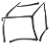
\includegraphics[height=\baselineskip]{figures/einheitswuerfel_rand}).

        \begin{behauptung*}
            \( f\maps M\to \reals \), \( x\mapsto \norm{x} \) ist stetig bezüglich \( \supnorm{\cdot} \).
        \end{behauptung*}
        \begin{subproof}
            \begin{align*}
                \abs{f(x)-f(y)}=\abs{\norm{x}-\norm{y}}\underset{(*)}{\leq}\norm{x-y}\leq C\supnorm{x-y}
            \end{align*}
            \( (*) \) umgekehrte Dreiecksungleichung:
            \begin{align*}
                \norm{x}-\norm{y}&=\norm{x+y-y}-\norm{y}\overset{\triangle}{\leq}\norm{x+y}\\
                \norm{y}-\norm{x}&=\norm{y+x-x}-\norm{x}\leq \norm{x+y}.
            \end{align*}
        \( M \) ist abgeschlossen bezüglich \( \supnorm{\cdot} \) (denn \( \reals^n\setminus M= \) Urbild der offenen Menge \( \reals\setminus \Set{1} \) unter der stetigen Abbildung \( x\mapsto \supnorm{\cdot} \)). \( M\subset  \) abgeschlossenen \emph{Quader} und dieser ist \emph{kompakt} in \( (\reals^n,\supnorm{\cdot}) \) (\thref{quader_ist_kompakt_norm_undendlich}) \timplies \( M \) ist kompakt (\ref{abgeschlossene_teilmenge_kompakter_menge_ist_kompakt}).

        Es folgt: \( f \) nimmt sein Minimum \( b \) an und (da \( f>0 \)) somit ist \( b>0 \). Nach Definition ist \( \norm{y}\geq b\quad \forall y\in M \). Für alle \( x\in \reals^n\setminus\Set{0} \) gilt \( \frac{x}{\supnorm{x}}\in M \), also ist \( \norm{\frac{x}{\supnorm{x}}}\geq b \), also \( \norm{x}\geq b\supnorm{x} \) und für \( x=0 \) gilt dies ohnehin.
        \end{subproof}
    \end{proofenumerate}
\end{proof}
\begin{lemma}\label{quader_ist_kompakt_norm_undendlich}
    Der Quader \( Q=\Set{x=(x_1,\dotsc, x_n)\in \reals^n| a_j\leq x_j\leq b_j} \) ist kompakt in \( \reals^n,\supnorm{\cdot} \) (\( a_j\leq b_j \)).
\end{lemma}
\begin{proof}
    Sei \( (U_j)_j \) eine offene Überdeckung von \( Q \). Angenommen, \( Q \) kann nicht durch endlich viele \( U_j \)'s überdeckt werden.

    Wir konstruieren induktiv eine Folge von abgeschlossenen Teilquadern
    \begin{align*}
        Q_0\supset Q_1\supset Q_2\supset \dotsb
    \end{align*}
    mit
    \begin{eigenschaftenenumerate}
        \item \( Q_n \) kann \emph{nicht} durch endlich viele \( U_j \)'s überdeckt werden
        \item \( \diameter-{Q_m}=2^{-m}\diameter-{Q} \).
    \end{eigenschaftenenumerate}
    \minisec{Beachte:} \( \diameter-{Q}= \) Länge der länsten Seite bezüglich \( \supnorm{\cdot} \).
    \begin{figure}[H]
        \centering
        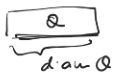
\includegraphics[width=0.3\linewidth]{figures/diameter_quader_norm_unendlich}
        \label{fig:diameter_quader_norm_unendlich}
    \end{figure}
    Setze \( Q_0=Q \). Sei \( Q_m \) konstruiert. Schreibe \( Q_m=I_1\times\dotsb\times I_n \), \( I_j \) abgeschlossene Intervalle. Zerlege \( I_j^{(1)}\cup I_j^{(2)} \) in zwei abgeschlossene Intervalle der halben Länge und setze
    \begin{align*}
        Q^{(s_1,\dotsc,s_n)}\definedas I_1^{(s_1)}\times\dotsb\times I_n^{(s_n)},\quad s_j\in \Set{1,2}.
    \end{align*}
    Das ergibt \( 2^n \) Quader mit
    \begin{align*}
        \bigcup_{s_j\in \Set{1,2}}Q_m^{(s_1,\dotsc,s_n)}=Q_m
    \end{align*}
    \begin{figure}[H]
        \centering
        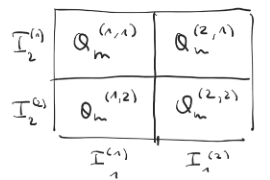
\includegraphics[width=0.5\linewidth]{figures/teilquader}
        \label{fig:teilquader}
    \end{figure}
    Es gibt mindestens einen Quader \( Q_m^{(s_1,\dotsc,s_n)} \), der nicht durch endlich viele \( U_j \)'s überdeckt werden kann. Einen solchen wählen wir als \( Q_{m+1} \). Es gilt per Konstruktion
    \begin{align*}
        \diameter{Q_{m+1}}=\frac{1}{2}\diameter{Q_m}=\frac{1}{2^{m+1}}\diameter{Q}.
    \end{align*}
    
    Nach dem Schachtelungsprinzip \texists \( a\in Q_m \) \tforall \( m \). Da \( (U_j)_j \) \( Q \) überdeckt \texists \( U_{j_0} \) \sd \( a\in U_{j_0} \). \( U_{j_0} \) offen \timplies \texists \( \varepsilon>0 \) \sd \( \ball;{\varepsilon}^{\supnorm{\cdot}}(a)\subset U_{j_0} \). Wähle \( m \) so groß, dass \( \diameter{Q_m}<\varepsilon \). \( a\in Q_m \) \timplies \( Q_m\subset \ball;{\varepsilon}^{\supnorm{\cdot}}(a)\subset U_{j_0} \) \contra Widerspruch Konstruktion der \( Q_m \).
\end{proof}
\begin{bemerkung}
    Aus \ref{r_alle_normen_aequivalent} folgt: \( Q \) ist bezüglich jeder Norm kompakt. Bolzano-Weierstraß (\ref{bolzanoweierstrass}) \timplies In \( (\reals^n,\norm{\cdot}) \) hat jede beschränkte Folge eine konvergente Teilfolge.
\end{bemerkung}
\begin{bemerkungen}
    Wir haben bereits gesehen:
    \begin{enumerate}
        \item Auf nicht endlich-dimensionalen Vektor-Räumen sind nicht alle Normen äquivalent:\\
        \( (\stetigefunktionen(\interval{a}{b}), \supnorm{\cdot}) \) ist vollständig, \( (\stetigefunktionen(\interval{a}{b}), \norm{\cdot}_{L^1}) \) nicht.
        \item Auf dem \( \reals^n \) sind nicht alle Metriken äquivalent: \( d_{\text{disc}} \) ist stärker als jede Norm (und nicht schwächer).
    \end{enumerate}
\end{bemerkungen}
\begin{satz}[Heine-Borel]\label{heineborel}
    Eine Teilmenge \( A\subset \reals^n \) ist genau dann kompakt, wenn sie abgeschlossen und beschränkt ist. (\( \reals^n \) hier und im Folgenden als normierter VR). 
\end{satz}
\begin{proof}
    \begin{proofdescription}
        \item[\hin] Hatten wir letztes Mal (\ref{kompakt:abgeschlossen_beschraenkt}) für Kompakte in metrischen Räumen bewiesen.
        
        \item[\rueck] It \( A \) beschränkt so ist \( A \) in einem Quader enthalten (denn \( \supnorm{x-y}\leq  \norm{x-y} \) somit \( \normdiameter{\supnorm{\cdot}}{A}\leq C\normdiameter{\norm{\cdot}}{A}<\infty \)). \( Q \) ist kompakt (bezüglich \( \supnorm{\cdot} \) somit bezüglich \( \norm{\cdot} \)).\( A \) abgeschlossen \timplies \( A \) kompakt (\ref{abgeschlossene_teilmenge_kompakter_menge_ist_kompakt}).
    \end{proofdescription}
\end{proof}
\begin{bemerkung*}
    \ref{heineborel} gilt nicht in unendlich-dimensionalen Vektorräumen:

    Betrachte in \( \ell_1, \norm{\cdot}_{\ell_1}=\sum_{k=0}^{\infty}\abs{x_k} \) die Folge \( (x^n)_n \) wobei \( x^n=(x^n_k)_k \) sei mit \( x^n_k=0 \) für \( n\neq k \) und \( (x^n)_n=1 \). Dann gilt \( \norm{x^n}_{\ell_1}=1 \) und
    \begin{align*}
        \norm{x^n-x^m}_{\ell_1}=2\quad \forall m\in \Set{0,1,\dotsc,n-1}.
    \end{align*}
    \timplies Die Folge besitzt keine konvergente Teilfolge, kann also (Bolzano-Weierstrass) nicht kompakt sein, obwohl \( \Set{x^n|n\in \naturals_0} \) beschränkt und abgeschlossen in \( (\ell_1, \norm{\cdot}_{\ell_1}) \) ist.
\end{bemerkung*}

% !TEX root = ./Vorlesungsmitschrift DIFF 2.tex  
\lecture{Mo 04.05. 10:15}{}
\section*{Stetige Abbildungen in normierten Vektorräumen}
\subsection*{Lineare Abbildungen}
\begin{satz}\label{lineare_abbildung:stetigkeitssatz}
    Seien \( (V,\norm{\cdot}_{V}) \) und \( (W,\norm{\cdot}_{W}) \) normierte Vektorräume.
    Sei \( A\maps V\to W \) linear.
    Dann sind folgende Aussagen äquivalent:
    \begin{eigenschaftenenumerate}
        \item \label{lineare_abbildung:stetigkeitssatz:stetig} \( A \) ist stetig
        \item \label{lineare_abbildung:stetigkeitssatz:stetig_in_null} \( A \) ist stetig in \( 0 \)
        \item \label{lineare_abbildung:stetigkeitssatz:norm_beschraenkt} \( \norm{A(x)}_{W}\leq C\norm{x}_{V} \).
    \end{eigenschaftenenumerate}
    
\end{satz}
\begin{proof}
    \begin{proofdescription}
        \item[\ref{lineare_abbildung:stetigkeitssatz:stetig} \timplies \ref{lineare_abbildung:stetigkeitssatz:stetig_in_null}] \checkmark
        \item[\ref{lineare_abbildung:stetigkeitssatz:stetig_in_null} \timplies \ref{lineare_abbildung:stetigkeitssatz:norm_beschraenkt}] \( A \) stetig in \( 0 \) \timplies zu \( \varepsilon=1 \) \texists \( \delta>0 \) \sd
        \begin{align*}
            \norm{A(y)-A(0)}_{W}\overset{\text{Lin}}{=}\norm{A(y)}_{W}<1\quad \forall y\in V \text{ mit }\norm{y-0}_{V}=\norm{Y}_V<\delta.
        \end{align*} 
        Setze \( C\definedas \quot{2}{\delta} \).
        Sei \( x\in V\setminus \zeroset \) beliebig (für \( x=0 \) gilt die Ungleichung \ref{lineare_abbildung:stetigkeitssatz:norm_beschraenkt} ohnehin).
        Setze \( \lambda\definedas \quot{1}{C\norm{x}_{V}} \) und \( y\definedas \lambda x \).
        
        Dann ist \( \norm{y}_V=\frac{1}{C\norm{x}_V}\norm{x}_V=\quot{\delta}{2}<\delta \), also \( \norm{A(y)}_W<1 \).
        \begin{align*}
            A(y)=A(\lambda x)=\frac{1}{C\norm{x}_V}A(x)\implies \Beh.
        \end{align*}
        \item[\ref{lineare_abbildung:stetigkeitssatz:norm_beschraenkt}\timplies \ref{lineare_abbildung:stetigkeitssatz:stetig}] Es gebe \( C>0 \) \sd
        \begin{align*}
            \norm{A(x)}_{W}\leq C\norm{x}_V \quad \forall x\in V.
        \end{align*} 
        Dann gilt insbesondere für \( x=y-a \).
        \begin{align*}
            \norm{A(x)}_{W}\explain{\text{Linearität}}{=}\norm{A(y)-A(a)}\leq C\norm{y-a}_{V}.
        \end{align*}
        Sei \( \varepsilon>0 \).
        Dann ist also
        \begin{align*}
            \norm{A(y)-A(a)}_{W}<\varepsilon\quad \forall y,a \text{ mit }\norm{y-a}_{V}<\frac{\varepsilon}{C}
        \end{align*}
        und somit ist \( A \) sogar gleichmäßig stetig.
    \end{proofdescription}    
\end{proof}
\begin{beispiele*}
    \begin{enumerate}
        \item \( (\stetigefunktionen(\interval{a}{b},\reals),\norm{\cdot}_{\infty}) \).
        \begin{align*}
            I\maps \stetigefunktionen(\interval{a}{b})\to \reals,\logicspace I(f)\definedas \Integrate{f(t)}{t,a,b}.
        \end{align*}
        \( I \) ist linear und es gilt
        \begin{align*}
            \norm{I(f)}\leq (b-a)\norm{f}_{\infty}
        \end{align*}
        \timplies \( I \) ist stetig.
        \item \( D\maps (\stetigefunktionen^1(\interval{a}{b}),\norm{\cdot}_{\infty})\to (\stetigefunktionen(\interval{a}{b}),\norm{\cdot}_{\infty}) \), \( D\maps f\mapsto f' \).
        \begin{behauptung*}
            \( D \) ist nicht stetig.
        \end{behauptung*}
        \begin{proof}[Denn:]
            \( D \) ist linear \checkmark, aber die Bedingung aus \thref{lineare_abbildung:stetigkeitssatz} ist verletzt: Betrachte \( f_n\in C^1(\interval{0}{2}) \), \( f_n=x^n    \).
            Dann ist \( \norm{f_n}_{\infty}=1 \), aber \( \norm{Df_n}_{\infty}=n \) \timplies es kann kein \( C>0 \) geben \sd
            \begin{align*}
                n=\norm{Df_n}_{\infty}\leq C\norm{f_n}=C\quad \forall n.
            \end{align*}
        \end{proof}
    \end{enumerate}
\end{beispiele*}
\begin{definition*}
    Seien \( V \) und \( W \) normierte Vektorräume.
    Sei \( A\maps V\to W \) lineare stetige Abbildung.
    Die \emph{Operatornorm} von \( A \) ist definiert als
    \begin{align*}
        \norm{A}_{\text{op}}\definedas \sup_{\substack{x\in V\\ x\neq 0}}\frac{\norm{Ax}_{w}}{\norm{x}_{V}}.
    \end{align*}
\end{definition*}
    Auf dem VR der stetigen linearen Funktionen \( V\to W \) ist \( \norm{\cdot}_{\text{op}} \) eine Norm.
    \( \norm{A}_{\text{op}} \) ist die kleinste Konstante für die noch die Abschätzunge aus \ref{lineare_abbildung:stetigkeitssatz} gilt und es folgt
\begin{bemerkung}
    Ein linearer Operator ist genau dann stetig, wenn gilt \( \norm{A}_{\text{op}}<\infty \).
\end{bemerkung}
\begin{beispiel*}
    Ist \( A\maps \reals^n \to \reals^m \) linear, so gilt 
    \begin{align*}
        A\in \Mat(m\times n,\reals)\simeq \reals^{m\cdot n}.
    \end{align*}
    Daher ist \( \norm{\cdot}_{\text{op}} \) in diesem Fall äquivalent zu in \( \norm{\cdot}_{\infty} \), \( \norm{A}_{\infty}=\max_{i,j}\abs{A_{ij}}<\infty \), insbesondere also schwächer und somit ist \( A \) stetig.

    Konkret gilt: Setze \( V=(\reals^n, \norm{\cdot}_{V}) \), \( W=(\reals^n,\norm{\cdot}_W) \).
    Sei \( y=Ax \) \timplies \( y_i=\sum_{j=1}^{n}A_{ij}x_j\) für \( i=1,\dotsc,m \).
    \begin{align*}
        &\norm{y}_{W}\begin{aligned}[t]
            &\overset{\triangle}{\leq}\sum_{i=1}^{m}\norm{y_i e_i}_{W}\\
            &\stackrel[\mathclap{\text{Hom}}]{\triangle}{\leq}\sum_{i,j}\abs{A_{ij}x_j}\norm{e_i}_{W}\\
            &=\sum_{i,j}\abs{A_{ij}}\cdot\abs{x_k}\cdot\norm{e_i}_{W}\\
            &\leq \norm{A}_{\infty}\cdot\norm{x}_{\ell^1}\cdot \underbrace{\sum_{i=1}^{m}\norm{e_i}_W}_{=c_W}
        \end{aligned}\\
        \implies &\norm{A}_{\text{op}}=\sup_{x\neq 0}\frac{\norm{Ax}_{W}}{\norm{x}_V}\leq \norm{A}_{\infty}\cdot C_W\cdot\underbrace{\sup_{x\neq 0}\frac{\norm{x}_{\ell^1}}{\norm{x}_V}},        
    \end{align*}
    wobei \( C_V \) eine Konstante ist mit
    \begin{align*}
        \norm{x}_{\ell^1}\leq C_V\cdot \norm{x}_V\quad \forall x\in V=\reals^n.
    \end{align*}
\end{beispiel*}
\begin{bemerkung}
    Unsere Beschränkung auf den \( \reals^n \) (statt beliebige endlich-dimensionale Vektorräume zuzulassen), bedeutet also keine Einschränkung, da ein Basiswechsel nach der Überlegung oben stetig ist.
\end{bemerkung}
\begin{beispiele}
    \( f\maps \reals^n\to \reals^m \).
    \begin{eigenschaftenenumerate}
        \item \emph{Kurven} \( \gamma\maps I\to \reals^n \), \( I \) Intervall, stetig.
        \begin{beispiele*}
            \item \( \gamma\maps \interval{0}{2\pi}\to \reals^2 \), \( t\mapsto (r \cos t, r \sin t) \), \( r>0 \).
            Stetigkeit: Wir versehen \( \reals^2 \) mit \( \norm{\cdot}_{\infty} \).
            Dann folgt die Stetigkeit von \( \gamma \) aus der Stetigkeit der Komponentenfunktionen \( I\to \reals \).
            \item \( \gamma\maps \reals\to \reals^2 \), \( t\mapsto (t^2-1,t^3-1) \) genauso.
            Spur von \( \gamma=\Set{\gamma(t)|t\in \reals} \)
            \begin{figure}[H]
                \centering
                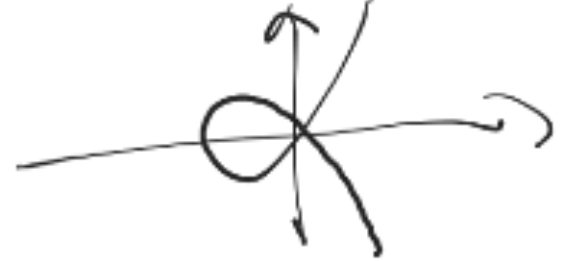
\includegraphics[width=0.5\linewidth]{figures/komponentenstetigkeit_beispiel_hoch_2_gegen_hoch_3}
                \label{fig:komponentenstetigkeit_beispiel_hoch_2_gegen_hoch_3}
            \end{figure}
        \end{beispiele*}
        \item Gebrochen rationale Funktionen:
        \begin{beispiele*}
            \item \( f\maps \reals^2\to \reals \).
            \begin{align*}
                f(x,y)=\begin{cases}
                    \frac{x^2y}{x^2+^2}&(x,y)\neq (0,0)\\
                    0&(x,y)=(0,0).
                \end{cases}                
            \end{align*}
            \( f \) ist stetig: auf \( \reals^2\setminus \zeroset \) sicherlich als Verknüpfung und Produkt stetiger Funktionen:
            \begin{align*}
                f=\text{Inv}\circ p_1\cdot p_2\quad \text{Inv}(t)=\frac{1}{t},\quad p_1(x,y)=x^2+y^2,\quad p_2(x,y)=x^2y.
            \end{align*}
            Stetigkeit in \( 0 \): Es gilt \( (x-y)^2\geq 0 \)
            \begin{align*}
                \implies &2\abs{xy}\leq x^2+y^2\\
                \implies &\abs{\frac{x^2y}{x^2+y^2}}<\frac{\abs{x}}{2}
            \intertext{für \( ((x_n,y_n))_{n} \), \( (x_n,y_n)\goesto(0,0) \) (bezüglich irgendeiner Norm) gilt insbesondere \( x_n\goesto 0 \)}
                \implies &\abs{f(x_n,y_n)-0}=\abs{\frac{x_n^2 y_n}{x_n^2+y_n^2}}<\frac{\abs{x_n}}{2}\goesto 0 \logicspace \text{in }\reals.
            \end{align*}
            \item \( f\maps \reals^2\to \reals \),
            \begin{align*}
                f(x,y)=\begin{cases}
                    \frac{x^2y}{x^4+y^2}&(x,y)\neq (0,0)\\
                    0&(x,y)=(0,0).
                \end{cases}
            \end{align*}
            \( f \) ist stetig auf \( \reals^2\setminus \zeroset \) (siehe oben).
            \( f \) ist nicht stetig in \( 0 \): Betrachte etwa \( (x_n,y-n)=\left( \frac{1}{n}, \frac{1}{n^2} \right) \), \( n\geq 1 \).
            Dann gilt
            \begin{align*}
                f(x_n,y_n)=\frac{1}{n^2n^2}\left( \frac{n^4}{2} \right)=\frac{1}{2}\cancel{\goesto}0.
            \end{align*}
            \minisec{Achtung:}
            Es gibt durchaus Folgen \( (x_n,y_n)\goesto 0 \) \sd \( f(x_n,y_n)\goesto 0 \) (für \( n\goesto \infty \)), \zb \( (x_n,y_n)=\left( 0,\frac{1}{n} \right) \), wo \( f\left( 0,\frac{1}{n} \right)=0\quad \forall n \) oder \( (x_n,y_n)=\left( \quot{1}{n},\quot{1}{n} \right) \) wo 
            \begin{align*}
                f(x_n,y_n)=\frac{1}{n^2}\left( \frac{n^2}{1+\quot{1}{n^2}} \right)\goesto 0.
            \end{align*}

            Daher muss man, wenn man Stetigkeit zeigen will, in Argument finden, dass für \emph{alle} Folgen funktioniert.
            \begin{figure}[H]
                \centering
                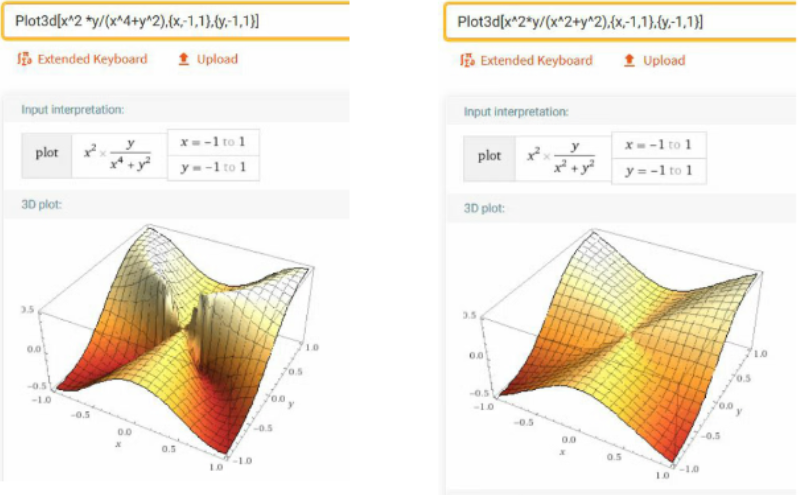
\includegraphics[width=\linewidth]{figures/contourplot_r_n_stetigkeit_beispiele}
                \caption*{Contour-Plot: Eingezeichnet werden alle \( (x,y) \), die die gegebene Gleichung erfüllen.
                Von Wolfram Alpha.}
                \label{fig:countourplot_r_n_stetigkeit_beispiele}
            \end{figure}
            \begin{figure}[H]
                \centering
                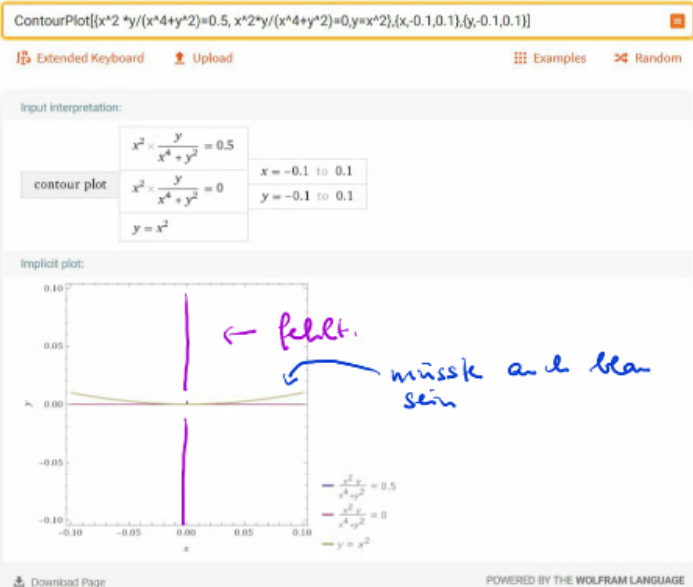
\includegraphics[width=\linewidth]{figures/contourplot_r_n_stetigkeit_beispiele_2_d}
                \label{fig:countourplot_r_n_stetigkeit_beispiele_2_d}
            \end{figure}
        \end{beispiele*}
    \end{eigenschaftenenumerate}
\end{beispiele}
\section*{Vektorräume mit Skalarprodukt}
Eine spezielle Klasse von Normen sind solche, die von einem sogenannten Skalarprodukt induziert werden.
\begin{definition}
    Sei \( V \) ein Vektorraum über \( \reals \).
    Ein \emph{Skalarprodukt} auf \( V \) ist eine Abbildung \( \scalarproduct{\cdot}{\cdot}\maps V\times V\to \reals \) mit
    \begin{eigenschaftenenumerate}
        \item \label{skalarprodukt:linear}Linear: \begin{align*}
            \scalarproduct{\lambda x+\mu y}{z}=\lambda\scalarproduct{x}{z}+\mu\scalarproduct{y}{z}\quad \forall x,y,z\in V,\logicspace \lambda,\mu\in \reals
        \end{align*}
        \item \label{skalarprodukt:symmetrisch}Symmetrisch: \begin{align*}
            \scalarproduct{x}{y}=\scalarproduct{y}{x} \forall x,y\in V
        \end{align*}
        \item \label{skalarprodukt:positiv_definit}Positiv definit: \begin{align*}
            \scalarproduct{x}{x}\geq 0 \text{ und } \scalarproduct{x}{x}=0\iff x=0. 
        \end{align*}
    \end{eigenschaftenenumerate}
    
\end{definition}
\begin{bemerkung*}
    Mit \ref{skalarprodukt:symmetrisch} folgt auch die Linearität im zweiten Argument.
\end{bemerkung*}
\begin{beispiele*}
    \begin{itemize}
        \item \( \reals^n \), \( \scalarproduct{x}{y}=\sum_{i=1}^{n}x_i y_i \): Euklidisches Skalarprodukt.
        \begin{figure}[H]
            \centering
            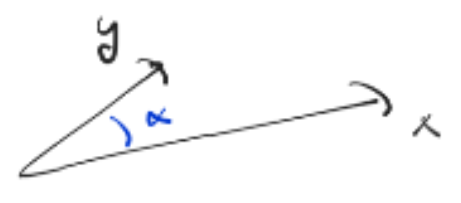
\includegraphics[width=0.3\linewidth]{figures/euklidisches_skalarprodukt_interpretation}
            \caption*{interpretation}
            \label{fig:euklidisches_skalarprodukt_interpretation}
        \end{figure}
        \( Y \) geht durch Drehstreckung aus \( x\neq 0 \) hervor:
        \begin{align*}
            y=\norm{y}_{\text{E}} \begin{pNiceMatrix} \cos \alpha & -\sin \alpha \\ \sin \alpha & \cos \alpha \end{pNiceMatrix} \frac{x}{\norm{x}_{\text{E}}}.
        \end{align*}
        Dann gilt:
        \begin{align*}
            \scalarproduct{x}{y}\begin{aligned}[t]
                &=\frac{\norm{y}_{\text{E}}}{\norm{x}_{\text{E}}}\scalarproduct{x}{\begin{pNiceMatrix} \cos \alpha x_1-\sin \alpha x_2 \\ \sin \alpha x_1+\cos \alpha x_2 \end{pNiceMatrix}}\\
                &=\frac{\norm{y}_{\text{E}}}(x_1^2\cos \alpha-\cancel{x_1 x_2\sin \alpha}+\cancel{x_1 x_2\sin \alpha+x_2^2\cos \alpha})\\
                &=\norm{y}_{\text{E}}\cdot\norm{x}{\text{E}}\cdot \cos \alpha.
            \end{aligned}            
        \end{align*}
        Das Skalarprodukt misst die Projektion von \( y \) auf \( x \)
        \begin{figure}[H]
            \centering
            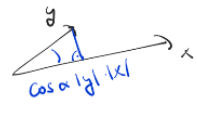
\includegraphics[width=0.3\linewidth]{figures/skalarprodukt_projektion_y_auf_x}
            \label{fig:skalarprodukt_projektion_y_auf_x}
        \end{figure}
        und umgekehrt
        \begin{figure}[H]
            \centering
            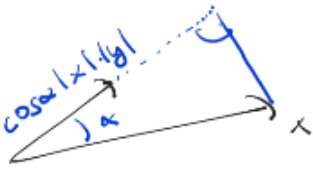
\includegraphics[width=0.3\linewidth]{figures/skalarprodukt_projektion_x_auf_y}
            \label{fig:skalarprodukt_projektion_x_auf_y}
        \end{figure}
        \item \( \reals^n \) mit \( \scalarproduct{x}{y}_W=\sum_{i=1}^{n}w_i x_i y_i \), \( w=(w_1,\dotsc, w_n) \) Gewichtsvektor, \( w_i>0 \).
        \item \( \reals^2 \) mit \( \scalarproduct{x}{y}\definedas 2x_1y_1-x_1y_2-x_2y_1+2x_2y_2 \) (zu überprüfen ist die Positive Definitheit).
        \item \emph{Kein} Skalarprodukt ist das Minkowski-Produkt: \( \reals^{n+1} \) mit \( ((x,y))\definedas x_0y_0-\sum_{i=1}^{n}x_i y_i \).

        Denn \( ((x,x))=0\iff x_0=\pm \norm{\underline{x}}_{\text{E}} \), \( x=(x_1,\dotsc,x_n) \).
        \item \( \stetigefunktionen(\interval{a}{b}) \) mit \( \scalarproduct{f}{g}=\Integrate{f(t)g(t)}{d,a,b} \).
    \end{itemize}
\end{beispiele*}
\begin{lemma}
    Sei \( V \) VR mit Skalarprodukt \( \scalarproduct{\cdot}{\cdot} \).
    Dann ist durch \( \norm{x}\definedas\sqrt{\scalarproduct{x}{x}} \) eine Norm auf \( V \) definiert.
\end{lemma}
\begin{proof}
    \begin{proofdescription}
        \item[\ref{norm:positiv_definit}] \( \norm{x=0}  \)\timplies \( \scalarproduct{x}{x}=0 \) \( \underset{\ref{skalarprodukt:positiv_definit}}{\implies} \), \( \norm{0}=0 \) \checkmark.
        \item[\ref{norm:betrags_homogen}] \( \norm{\lambda x}=\sqrt{\lambda^2\scalarproduct{x}{x}}=\abs{\lambda}\sqrt{\scalarproduct{x}{x}} \) \tforall \( \lambda\in \reals \), \( x\in V \).
        \item[\ref{norm:dreiecksungleichung}] 
        \begin{align*}
            \norm{x+y}^2 \begin{aligned}[t]
                &=\scalarproduct{x+y}{x+y}\\
                &=\norm{x}^2+2\scalarproduct{x}{y}+\norm{y}^2\\
                &\leq \norm{x}^2+2\abs{\scalarproduct{x}{y}}+\norm{y}^2\\
                &\explain{\text{siehe \eqref{eq:cauchy_schwarzsche_ungeleichung} unten}}{\leq} (\norm{x}+\norm{y})^2\implies \triangle,
            \end{aligned}            
        \end{align*}
        denn die Wurzel ist monoton wachsend.

        Es gilt die \emph{Cauchy-Schwarzsche} Ungleichung:
        \begin{align*}
            \tag{*}\label{eq:cauchy_schwarzsche_ungeleichung} \abs{\scalarproduct{x}{y}}\leq \norm{x}\cdot \norm{y}.
        \end{align*}
        \begin{subproof}
            \begin{align*}
                0\leq \scalarproduct{x-\lambda y}{x-\lambda y}=\norm{x}^2-2\lambda \scalarproduct{x}{y}+\lambda^2 \norm{y}^2\quad \forall x,y\in V\logicspace \lambda\in\reals,
            \end{align*}
            also speziell für \( y\neq 0 \) (für \( y=0 \) gilt die Ungleichung sowieso) und \( \lambda=\frac{\scalarproduct{x}{y}}{\norm{y}^2} \):
            \begin{align*}
                0\leq \norm{x}^2-\frac{\scalarproduct{x}{y}^2}{\norm{y}^2}.
            \end{align*}
        \end{subproof}
    \end{proofdescription}
\end{proof}
Einen Vektorraum mit Skalarprodukt betrachten wir immer als mit der von Skalarprodukt induzierten Norm, also Metrik, also Topologie.

Nicht jede Norm wird von einem Skalarprodukt induziert. Es gilt
\begin{lemma}
    Sei \( (V,\norm{\cdot}) \) normierter VR\@ Dann wird \( \norm{\cdot} \) von einem Skalarprodukt induziert genau dann, wenn die Parallelogramm-Gleichung gilt:
    \begin{align*}
        \norm{x+y}^2-\norm{x-y}^2=2(\norm{x}^2+\norm{y}^2)\quad \forall x,y\in V.
    \end{align*}
    \begin{figure}[H]
        \centering
        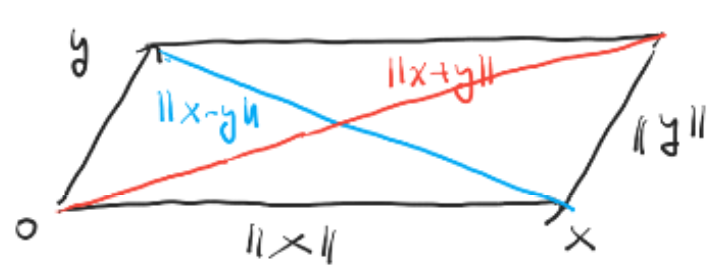
\includegraphics[width=0.5\linewidth]{figures/parallelogramm_gleichung_namenserklaerung}
        \caption*{Erklärung für den Namen. \( \reals^2 \), \( \norm{\cdot}=\norm{\cdot}_{\text{E}} \).}
        \label{fig:parallelogramm_gleichung_namenserklaerung}
    \end{figure}    
\end{lemma}
\begin{proof}
    \begin{proofdescription}
        \item[\hin] Sei \( \norm{x}=\sqrt{\scalarproduct{x}{x}} \). Dann gilt
        \begin{align*}
            \norm{x+y}^2+\norm{x-y}^2 \begin{aligned}[t]
                &=\scalarproduct{x+y}{x+y}+\scalarproduct{x-y}{x-y}\\
                &=2\norm{x^2}+0+2\norm{y^2}.
            \end{aligned}
        \end{align*}
        \item[\rueck] Erfülle \( \norm{\cdot} \) die Parallelogramm-Gleichung.
        \begin{behauptung*}
            Durch \enquote{Polarisation}, also
            \begin{align*}
                \scalarproduct{x}{y}\definedas \frac{1}{4}(\norm{x+y}^2-\norm{x-y}^2)
            \end{align*}
            ist ein Skalarprodukt definiert mit \( \norm{x}=\sqrt{\scalarproduct{x}{x}} \).
        \end{behauptung*}
        \begin{subproof}
            \begin{proofdescription}
                \item[2.\@ \Beh:] \( \scalarproduct{x}{x}=\frac{1}{4}\norm{2x}^2 \) \checkmark.
                \item[1.\@ \Beh:] \begin{itemize}
                    \item Aus der 2.\@ \Beh folgt die positive Definitheit aus der Nichtausgeartetheit und Positivität der Norm.
                    \item Die Symmetrie folgt sofort aus der Definition.
                    \item Linearität. Wir zeigen zunächst Additivität:
                    \begin{enumerate}[label=\rechtsklammer{\arabic*}]
                        \item \( \scalarproduct{x+u}{y}+\scalarproduct{x-u}{y}=\scalarproduct{x}{y} \)
                        \begin{subproof}[denn:]
                            \begin{align*}
                                \text{linke Seite}\begin{aligned}[t]
                                    &=\frac{1}{4}(\begin{aligned}[t]
                                        &\norm{x+u+y}^2-\norm{x+u-y}^2\\
                                        &+\norm{x-u+y}^2-\norm{x-u-y}^2
                                    \end{aligned}
                                    )\\
                                    &\explain{\text{Parallelogramm-Gleichung}}{=}\frac{1}{2}(\norm{x+y}^2+\norm{u}^2-\norm{x-y}^2-\norm{u}^2)\\
                                    &=\frac{1}{2}(\scalarproduct{x+y}{x+y}-\scalarproduct{x-y}{x-y})\\
                                    &=2\scalarproduct{x}{y}.
                                \end{aligned}
                            \end{align*}
                        \end{subproof}
                        Damit auch gleich gezeigt:
                        \item \label{norm_hat_skalarprodukt:beweis:zwei_multiplikativitaet}\( \scalarproduct{2x}{y}=2\scalarproduct{x}{y} \) (setze \( u=x \)) und mit \( x=u+v \), \( y=u-v \) folgt
                        \item \label{norm_hat_skalarprodukt:beweis:additivitaet}Additivität:
                        \begin{align*}
                            \scalarproduct{x}{y}+\scalarproduct{y}{z}\begin{aligned}[t]
                                &=\scalarproduct{u+v}{z}+\scalarproduct{u-v}{z}\\
                                &=2\scalarproduct{u}{z}\\
                                &\underset{\ref{norm_hat_skalarprodukt:beweis:zwei_multiplikativitaet}}{=}\scalarproduct{2u}{z}\\
                                &=\scalarproduct{x+y}{z}
                            \end{aligned}
                        \end{align*}
                        \item \label{norm_hat_skalarprodukt:beweis:natuerliche_multiplikativitaet}per Induktion \( \scalarproduct{nx}{y}=n\scalarproduct{x}{y} \) \tforall \( n\in \naturals \), denn
                        \begin{align*}
                            \scalarproduct{(n+1)x}{y}\begin{aligned}[t]
                                &=\scalarproduct{nx+x}{y}\\
                                &\overset{\ref{norm_hat_skalarprodukt:beweis:additivitaet}}{=}\scalarproduct{nx}{y}+\scalarproduct{x}{y}\\
                                &\overset{\text{IV}}{=}n\scalarproduct{x}{y}+\scalarproduct{x}{y}\\
                                &=(n+1)\scalarproduct{x}{y}.
                            \end{aligned}
                        \end{align*}
                        \item \label{norm_hat_skalarprodukt:beweis:negativ_natuerliche_multiplikativitaet} Für \( \lambda\in -\naturals_0 \) gilt
                        \begin{align*}
                            \lambda\scalarproduct{x}{y}-\scalarproduct{\lambda x}{y}\begin{aligned}[t]
                                &=\lambda\scalarproduct{x}{y}-\scalarproduct{\abs{\lambda}(-x)}{y}\\
                                &=\lambda\scalarproduct{x}{y}-\abs{\lambda}\scalarproduct{-x}{y}\\
                                &=\lambda(\scalarproduct{x}{y}+\scalarproduct{-x}{y})\\
                                &=0
                            \end{aligned}
                        \end{align*}
                        \item Für \( \lambda\in \rationals \), \( \lambda=\quot{m}{n} \), \( m,n\in \wholes \):
                        \begin{align*}
                            n\scalarproduct{\frac{m}{n}x}{y}\underset{\ref{norm_hat_skalarprodukt:beweis:natuerliche_multiplikativitaet},\ref{norm_hat_skalarprodukt:beweis:negativ_natuerliche_multiplikativitaet}}{=}\scalarproduct{mx}{y}=m\scalarproduct{x}{y}.
                        \end{align*}
                        \item Für \( \lambda\in \reals \) existiert \( (\lambda_n)_n\subset \rationals \), \( \lambda_n\goesto \lambda \). Da \( \norm{\cdot} \) stetig ist, so auch \( \scalarproduct{\cdot}{\cdot} \)
                        \begin{align*}
                            \scalarproduct{\lambda x}{y}\begin{aligned}[t]
                                &=\scalarproduct{\lim \lambda_n x}{y}\\
                                &=\lim \scalarproduct{\lambda_n x}{y}\\
                                &=\lim \lambda_n \scalarproduct{x}{y}\\
                                &=\lambda\scalarproduct{x}{y}.
                            \end{aligned}
                        \end{align*}
                        Symmetrie \timplies es genügt, das erste Argument zu untersuchen.
                    \end{enumerate}
                \end{itemize} 
            \end{proofdescription}
        \end{subproof}
    \end{proofdescription}
\end{proof}
\begin{beispiel*}
    \( \norm{\cdot}_{\text{max}} \) wird nicht von einem Skalarprodukt induziert: Sei \( x=e_1\), \( y=e_2 \). Dann gilt:
    \begin{align*}
        \norm{e_1+e_2}^2_{\text{max}}+\norm{e_1-e_2}^2_{\text{max}}=1+1=2,
    \end{align*}
    aber
    \begin{align*}
        2(\norm{e_1}^2_{\text{max}}+\norm{e_2}^2_{\text{max}})=4.
    \end{align*}
\end{beispiel*}

% !TEX root = ./Vorlesungsmitschrift DIFF 2.tex  
\chapter{Differenzierbarkeit in \texorpdfstring{\( \reals^n \)}{R\^n}}
\lecture{Do 07.05. 10:15}{}
\begin{erinnerung*}
    Approximation einer Funktion \( f\maps \reals\to \reals \), die in \( a\in \reals \) differenzierbar ist, durch eine (affin) lineare Funktion
    \begin{align*}
        f(x)=f(a)+m_a(x-a)+R_a(x)
    \end{align*}
    mit \( R_a\maps \reals\to \reals \) und \( \lim_{x \goesto a}\frac{R_a(x)}{x-a}=0 \).

    Gibt es ein solches \( R_a \), so ist \( m_a \) eindeutig festgelegt und es gilt
    \begin{align*}
        m_a=\lim_{x \goesto a}\underbrace{\frac{f(x)-f(a)}{x-a}}_{\text{Differenzenquotient}}.
    \end{align*}
    \( f'(a)\definedas m_a \) heißt \emph{Ableitung} von \( f \) an der Stelle \( a \).
    \begin{figure}[H]
        \centering
        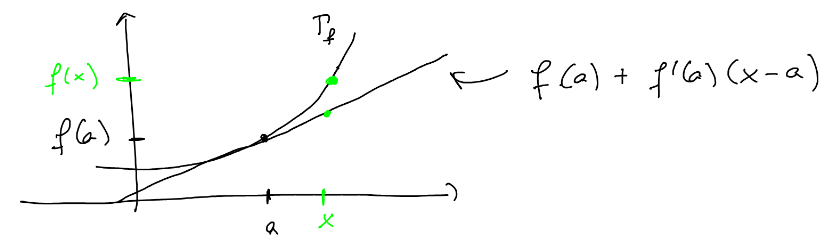
\includegraphics[width=0.7\linewidth]{figures/ableitung_erinnerung}
        \label{fig:ableitung_erinnerung}
    \end{figure}
    Für Abbildungen \( f\maps \reals^n\to \reals^n \) kann man analog definieren:
\end{erinnerung*}
\begin{definition}
    Die \emph{Ableitung} einer Funktion \( f\maps U\to \reals^m \), \( U\subset \reals^n \) offen, an der Stelle \( a\in U \), ist, wenn sie existiert, eine Matrix \( \totalderivative-{f}(a)\in \Mat(m\times n) \), die eine lineare Approximation von \( f \) ergibt:
    \begin{align*}
        f(x)=f(a)+\totalderivative-{f}(a)\explain{\text{Matrix-Multiplikation}}{\matrixmult}(x-a)+R_a(x)\tag{\(*\)}\label{eq:ableitung:definition}
    \end{align*}
    Sie existiert genau dann, wenn
    \begin{align*}
        \overset{\underset{\downarrow}{\text{in }\reals^m}}{\lim_{x\explain{\text{in }\reals^n}{\goesto} a}}\frac{R_a(x)}{\explain[big]{\text{eine Norm in \( \reals^n \)}}{\norm{x-a}}}=0
    \end{align*}
    und ist in diesem Fall eindeutig durch \eqref{eq:ableitung:definition} bestimmt und man sagt, \( f \) ist \emph{differenzierbar}.
\end{definition}
\begin{bemerkungen*}
    \begin{enumerate}
        \item Für \( n=m=1 \) stimmt die Definition mit der Üblichen überein, da \( \frac{R_a(x)}{x-a}\goesto 0 \) \tiff \( \frac{R_a(x)}{\abs{x-a}}\goesto 0 \).
        \item Eindeutigkeit: Sei \( A \) \sd
        \begin{align*}
            f(x)\begin{aligned}[t]
                &=f(a)+A\matrixmult(x-a)+\tilde{R}_a(x)\\
                &=f(a)+\totalderivative-{f}(a)\matrixmult (x-a)+R_a(x)
            \end{aligned}            
        \end{align*}
        Dann folgt:
        \begin{align*}
            \lim_{x \goesto a}(\underbrace{(A-\totalderivative-{f}(a))\matrixmult (x-a)\cdot\quot{1}{\norm{x-a}}}_{=\frac{1}{\norm{x-a}}(R_a(x)-\tilde{R}_a(x))})=0.
        \end{align*}
        \timplies \( A-\totalderivative-{f}(a)=0 \) (Nullmatrix), da wegen der Stetigkeit linearer Abbildungen \( \reals^n\to \reals^m \) der Grenzwert gleich \( (A-\totalderivative-{f}(a))\matrixmult \lim \quot{(x-a)}{\norm{x-a}} \) ist und \( \norm{\lim \quot{(x-a)}{\norm{x-a}}}=1\neq 0 \).
        \item Wie in der \diff{1} ist es oft zweckmäßig \( f \) an der Stelle \( a+h \) mit \( f \) an der Stelle \( a \) zu vergleichen (\( x=a+h \)).
        \begin{align*}
            f(a+h)=f(a)+\totalderivative-{f}(a)\matrixmult h+\underline{R}_h(a)
        \end{align*}
        mit \( \lim_{h \goesto 0}\quot{(\underline{R}_h(x))}{\norm{h}}=0 \).
    \end{enumerate}
\end{bemerkungen*}
\begin{beispiele*}
    \begin{enumerate}
        \item \( f\maps \reals^n\to \reals^n \), \( f(x)=A\matrixmult x+b \), \( A\in \Mat(m\times n, \reals) \), \( b\in \reals^m \).
        \begin{align*}
            f(a+h)=f(a)+A\matrixmult h\implies \totalderivative-{f}(a)=A.
        \end{align*}
        Insbesondere verschwindet die Ableitung einer konstanten Funktion.
    \item \( f\maps \reals^n \to \reals\), \( f(x)=\scalarproduct{x}{B\matrixmult x} \), \( \scalarproduct{\cdot}{\cdot} \) euklidisches Skalarprodukt, \( B\in \Mat(n\times n, \reals) \).
    \begin{align*}
        f(a+h)\begin{aligned}[t]
            &=\scalarproduct{a+h}{B\matrixmult (a+h)}\\
            &=\scalarproduct{a}{B\matrixmult a}+\scalarproduct{h}{B\matrixmult a}+\scalarproduct{a}{B\matrixmult h}+\scalarproduct{h}{B\matrixmult h}\\
            &\explain{\text{CHECK!}}{=}\scalarproduct{a}{B\matrixmult a}+\scalarproduct{(B+B^T)\matrixmult a}{h}+\scalarproduct{h}{Bh}. 
        \end{aligned}                
    \end{align*}
    Wegen (wähle \( \norm{\cdot}=\norm{\cdot}_{\text{E}} \))
    \begin{align*}
        \frac{\scalarproduct{a}{Bh}}{\norm{h}}\underset{\text{C-S}}{\leq}\frac{\norm{h}\cdot\norm{Bh}}{\norm{h}}\leq \norm{B}_{\text{op}}\cdot\norm{h}\goesto 0  \text{ für }h\goesto 0
    \end{align*}
    folgt: \( f \) ist in allen \( a\in \reals^n \) differenzierbar und
    \begin{align*}
        &\totalderivative-{f}(a)\matrixmult h=\scalarproduct{(B+B^T)\matrixmult a}{h}=(b_1,\dots,b_n)\begin{pNiceMatrix} h_1 \\ \vdots \\ h_n \end{pNiceMatrix}\\
        \implies &\totalderivative-{f}(a)=b=((B+B^T)\matrixmult a)^T\in \Mat(1\times n,\reals)\quad \forall h\in \reals^n. 
    \end{align*}
    \end{enumerate}
\end{beispiele*}
Aus der Definition folgt sofort
\begin{satz}
    Sei \( f\maps U\to \reals^m \), \( U\subset \reals^n \) offen, in \( a\in U \) differenzierbar. Dann ist \( f \) in \( a \) stetig.
\end{satz}
\begin{proof}
    \begin{align*}
        \lim_{h \goesto 0}f(a+h)\begin{aligned}[t]
            &=\lim_{h \goesto 0}(f(a)+\totalderivative-{f}(a)+\underline{R}_a(h))\\
            &=f(a)+\explain[Big]{\explain{\text{Norm in \( \reals^m \)}}{\norm{\totalderivative-{f}(a)\matrixmult h}}\leq \norm{\totalderivative-{f}(a)}_{\text{op}}\cdot\explain{\text{Norm in \( \reals^n \)}}{\norm{h}}}{0}+\explain{\phantom{\text{Es gilt sogar meeehr!}}\text{Es gilt sogar \(\quot{\underline{R}_a(h)}{\norm{h}}\goesto 0\)}}{0}
        \end{aligned}
    \end{align*}
\end{proof}
\begin{satz}[Kettenregel]
    Seien \( U\subset \reals^n \), \( V\subset \reals^m \) offen, \( g\maps U\to \reals^m \), \( f\maps V\to \reals^k \), \( g(U)\subset V \). Ist \( g \) in \( a\in U \) differenzierbar und \( f \) in \( b=g(a) \), so ist die Verkettung \( f\circ g\maps U\to \reals^k \) in \( a \) differenzierbar und es gilt
    \begin{align*}
        \totalderivative{f\circ g}(a)=\explain{\in \Mat(k\times m,\reals)}{\underbrace{\totalderivative-{f}(g(a))}}\explain[big]{\in \Mat(m\times n),\reals}{\underbrace{\totalderivative-{g}(a)}}.
    \end{align*}
\end{satz}
\begin{proof}
    \begin{align*}
        g(a+u)&=g(a)+A\cdot u+\underline{R}_a^g(u)\quad A=\totalderivative-{g}(a)\tag{1}\label{eq:ableitung:kettenregel:g}\\
        f(b+v)&=f(b)+B\cdot v+\underline{R}_b^f(v)\quad B=\totalderivative-{f}(b)\tag{2}\label{eq:ableitung:kettenregel:f}
    \end{align*}
    Setze speziell \( v\definedas g(a+u)-g(a)\overset{\eqref{eq:ableitung:kettenregel:g}}=A\cdot u+\underline{R}_a^g(u) \).
    \begin{align*}
        \implies f\circ g(a+u)\begin{aligned}[t]
            &=f(g(a+u))=f(g(a)+v)\eqstep{\text{Def } v}\\
            &\underset{\eqref{eq:ableitung:kettenregel:f}}{=}f(g(a))+B\matrixmult v+\underline{R}_b^f(v)\eqstep[p,v]{b=g(a)}\\
            &\explain{\text{Def \( v \) und \eqref{eq:ableitung:kettenregel:g}}}{=}f(g(a))+B\matrixmult A\matrixmult u+\explain{\text{zu zeigen: }\frac{\cdot}{\norm{u}}\goesto 0 \text{ für }u\goesto 0}{\underbrace{B\cdot\underline{R}_a^g(u)+\underline{R}_b^f(A\cdot u+\underline{R}_a^g(u))}}.
        \end{aligned}        
    \end{align*}
    \begin{itemize}
        \item \(\frac{\underline{R}_a^g(u)}{\norm{u}}\goesto 0 \) \timplies \texists \( C>0 \) \sd \( \norm{\underline{R}_a^g(n)}\leq C\norm{n} \).
        \item \( \frac{\underline{R}_b^f(v)}{\norm{v}}\goesto 0 \) \timplies \texists \( \underline{r}_b^f \) \sd \( \underline{R}_b^f(v)=\norm{v}\underline{r}_b^f(v) \)mit \( \underline{r}_b^f(v)\goesto 0 \) (\( v\goesto 0 \)).
    \end{itemize}
    \begin{align*}
        \implies &\explain{\text{Norm in \( \reals^k \)}}{\underline{R}_b^f(A\matrixmult u +\underline{R}_a^g(u))}\leq \explain{\text{Norm in \( \reals^k \)}}{\overbrace{A\matrixmult u +\underline{R}_a^g(u)}^{\leq\left( \norm{A}_{\text{op}}+C \right)\norm{u}}}\cdot\norm{\underline{r}_b^f(\underbrace{Au+\underline{R}_a^g(u)}_{\mathclap{\goesto 0 \text{ für }u\goesto 0}})}\\
        \implies &\frac{\underline{R}_b^f(A\matrixmult u+\underline{R}_a^g(u))}{\norm{u}}\goesto 0\quad (u\goesto 0).
    \end{align*}
\end{proof}
\begin{satz}[Produktregel, Quotientenregel]
    Seien \( f,g\maps U\to \reals \), \( U\subset \reals^n \) offen, differenzierbar in \( a\in U \). Dann gilt
    \begin{enumerate}
        \item \label{produktregel} \( f\cdot g \) ist differenzierbar in \( a \) und es gilt
        \begin{align*}
            \totalderivative{f\cdot g}(a)=\totalderivative-{f}(a)\matrixmult g(a)+f(a)\matrixmult \totalderivative-{g}(a).
        \end{align*}
        \item \label{quotientenregel} Ist \( g(a)\neq 0 \) so gilt: \( \quot{f}{g} \) ist auf einer Umgebung von \( a \) definiert und differenzierbar in \( a \) und es gilt 
        \begin{align*}
            \totalderivative{\quot{f}{g}}(a)=\totalderivative-{f}(a)\cdot\frac{1}{g(a)}-f(a)\cdot\frac{1}{g(a)^2}\cdot \totalderivative-{g}(a).
        \end{align*}
    \end{enumerate}
    
\end{satz}
\begin{proof}
    \begin{proofdescription}
        \item[\ref{produktregel}]
        \begin{align*}
            f(a+h)&=f(a)+\totalderivative-{f}(a)\matrixmult h+\underline{R}_{a}^f(h)\\
            g(a+h)&=g(a)+\totalderivative-{g}(a)\matrixmult h+\underline{R}_{a}^g(h)\\
            f\cdot g(a+h)&\begin{aligned}[t]
                &=\left( f(a)+\totalderivative-{f}(a)\matrixmult h+\underline{R}_{a}^f(h) \right)\left( g(a)+\totalderivative-{g}(a)\matrixmult h+\underline{R}_{a}^g(h) \right)\\
                &=\begin{aligned}[t]
                    &f(a)\cdot g(a)+(\underbrace{\totalderivative-{f}(a)\matrixmult g(a)}_{\in \Mat(1\times n,\reals)})\matrixmult h+(\underbrace{f(a)\matrixmult \totalderivative-{g}(a)}_{\in \Mat(1\times n,\reals)})\matrixmult h\\
                    &+\underbrace{(\totalderivative-{f}(a)\matrixmult h+\underline{R}_a^f(h))(\totalderivative-{g}(a)\matrixmult h+\underline{R}_a^g(h))}_{\frac{\cdot}{\norm{h}}\goesto 0 \text{ für }h\goesto 0}.
                \end{aligned}
            \end{aligned}            
        \end{align*}
        \item[\ref{quotientenregel}] \( g \) ist in \( a \) stetig \timplies \texists Umgebung von \( a \) \sd \( g(x)\neq 0 \) \tforall \( x\in U \) (wie in der \diff{1}: Sei \obda \( g(a)>0 \). Sei \( \varepsilon\definedas \quot{g(a)}{2} \). Sei \( \norm{\cdot} \) irgendeine Norm auf \( \reals^n \). Dann gibt es ein \( \delta>0 \) \sd
        \begin{align*}
            &\abs{g(x)-g(a)}<\varepsilon\quad \forall x\in B_{\delta}^{\norm{\cdot}}(a)\\
            \implies &-\frac{g(a)}{2}<g(x)-g(a)<\frac{g(a)}{2}\quad \forall x\in B_{\delta}^{\norm{\cdot}}(a),
        \end{align*}
        also \( 0<\frac{g(a)}{2}<g(x)<\frac{3}{2}\frac{g(a)}{2} \).) \timplies Auf \( U \) ist \( \quot{f}{g} \) wohldefiniert. Die Berechnung der Ableitung ist analog zu \ref{produktregel}, nachdem man sich überlegt hat, dass
        \begin{align*}
            \frac{1}{g}=\text{Inv}\circ g,\quad \text{Inv}(t)=\frac{1}{t}
        \end{align*}
        und somit nach der Kettenregel
        \begin{align*}
            \totalderivative*{\frac{1}{g}}(a)=\totalderivative-{\text{Inv}(g(a))}\cdot \totalderivative-{g}(a)
        \end{align*}
        und \( D \text{Inv}(t)=-\frac{1}{t^2} \) (\diff{1}).
    \end{proofdescription}    
\end{proof}
\section*{Geometrische Anschauung, partielle Ableitung}
\diff{1}: Ableitung beschreibt Rate der Veränderung. Höher-dimensional: Sei \( f\maps U\to \reals \), \( U\subset \reals^n \). Betrachte den Graph \( \Gamma_f=\Set{(x,f(x))|x\in U} \) (\vgl die Diskussion bei \ref{stetigkeit:beispiel:gebrochen_rationale_funktionen})
\begin{figure}[H]
    \centering
    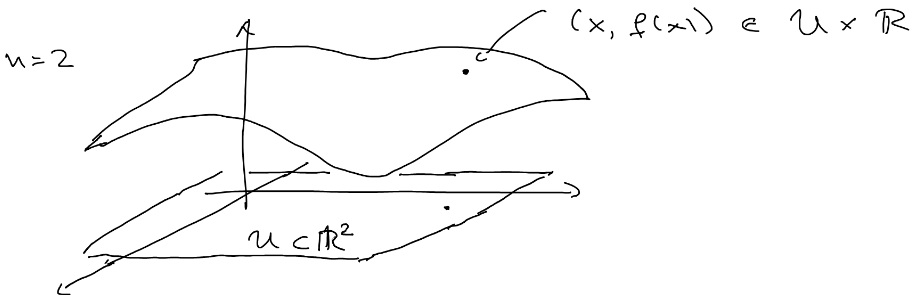
\includegraphics[width=0.8\linewidth]{figures/r2_zu_r_funktion_veranschaulichung}
    \label{fig:r2_zu_r_funktion_veranschaulichung}
\end{figure}
\begin{definition*}[Niveau-Mengen]
    Zu \( c\in \reals \) setze \( N_f(c)\definedas \Set{x\in U|f(x)=c} \).
\end{definition*}
\begin{beispiel*}
    \begin{figure}[H]
        \centering
        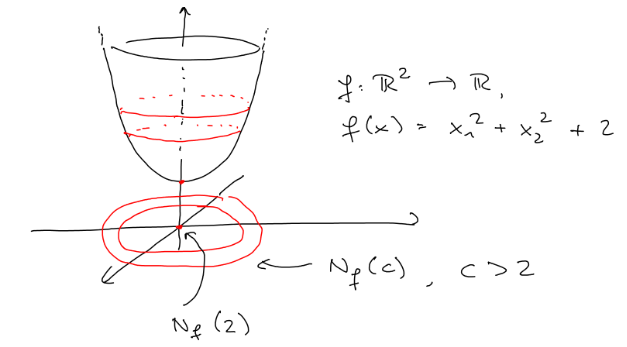
\includegraphics[width=0.5\linewidth]{figures/niveau_menge_beispiel}
        \caption*{Es gilt \( N_f(c)=\emptyset \) für \( c<2 \).}
        \label{fig:niveau_menge_beispiel}
    \end{figure}
    Entlang der Niveauflächen ist \( f \) konstant. Wie wird das in der Ableitung sichtbar?

    Im Beispiel oben ist \( \totalderivative-{f}(a)=(2a_1,2a_2) \) (check!). Sei \( a=(r\cos \phi, r\sin \phi) \), \( r>0 \). Betrachte \( f(a+h)=f(a)+\totalderivative-{f}(a)\matrixmult h+\underline{R}_a(h) \). Ist \( h=\textcolor{Blue}{(-\varepsilon \sin \phi, \varepsilon \cos \phi)} \), \( \varepsilon>0 \) (in \enquote{Richtung} der Niveaumenge), so ist \( \totalderivative-{f}(a)\matrixmult h=0 \).
    \begin{figure}[H]
        \centering
        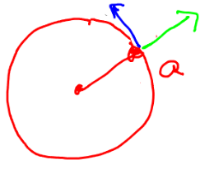
\includegraphics[width=0.2\linewidth]{figures/in_richtung_und_orthogonal_der_niveaumenge}
        \label{fig:in_richtung_und_orthogonal_der_niveaumenge}
    \end{figure}
    Ist dagegen \( h=\textcolor{Green}{(\varepsilon \cos \phi, \varepsilon \sin \phi)} \) (von der Niveaumenge weg), so ist \( \totalderivative-{f}(a)\matrixmult h=2r\varepsilon>0 \). Das wollen wir im Folgenden systematisch studieren.
\end{beispiel*}
\begin{definition*}
    Sei \( f\maps U\to \reals^m \), \( U\subset \reals^n \) offen, gegeben. Für \( a\in U \) und \( v\in \reals^n \) heißt der Grenzwert (falls er existiert)
    \begin{align*}
        \partial_v f(a)\definedas \explain{\text{in \( \reals^m \)}}{\lim_{t \goesto 0}}\frac{f(a+tv)-f(a)}{t}
    \end{align*}
    die \emph{Richtungsableitung von \( f \)} in \( a \) in Richtung \( v \).
    \begin{figure}[H]
        \centering
        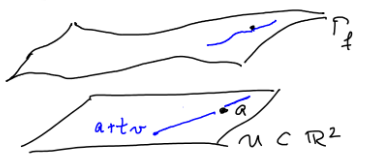
\includegraphics[width=0.5\linewidth]{figures/richtungsableitung}
        \label{fig:richtungsableitung}
    \end{figure}
\end{definition*}
\begin{bembspe}
    \begin{enumerate}
        \item \( \partial_v f(a)=\evaluateat{\frac{d}{dt}}{t=0} g_{a,v}(t)=g_{a,v}'(0) \), \( g_{a,v}(t)=f(a+tv) \).
        \item \( f=(f_1,\dotsc,f_m)^T \), so gilt
        \begin{align*}
            \partial_v f(a)=(\partial_v f_1(a),\dotsc, \partial_v f_m(a))^T
        \end{align*}
            \item \( f\maps (x_1,x_2)\mapsto x_1^2+x_2^2+2 \). Sei \( a=(r\cos \phi, r\sin \phi) \). Ist \( v=(\varepsilon \cos \phi, \varepsilon\sin \phi) \), so ist
            \item \begin{align*}
                g_{a,v}(t)=((r+\varepsilon t)\cos \phi)^2+((r+\varepsilon t)\sin \phi)^2+2
            \end{align*}
            und somit \( \partial_v f(a)=g_{a,v}'(0)=2(r+\varepsilon \cdot 0)\varepsilon=2r\varepsilon \).
            
            Ist \( v=(-\varepsilon \sin \phi, \varepsilon \cos \phi) \), so ist
            \begin{align*}
                g_{a,v}(t)=(r \cos \phi-\varepsilon t\sin \phi)^2+(r\sin \phi+\varepsilon t \cos \phi)^2
            \end{align*}
            und somit
            \begin{align*}
                \partial_v f(a)=g_{a,v}'(0)=2(r\cos \phi-0)(-\varepsilon \sin \phi)+2(r\sin \phi+0)(\varepsilon \cos \phi)=0.
            \end{align*}
            Das ist kein Zufall, denn es gilt
    \end{enumerate}
\end{bembspe}
\begin{satz}
    Sei \( f\maps U\to \reals^m \), \( U\subset \reals^n \) offen, in \( a\in U \) differenzierbar. Dann besitzt \( f \) die Richtungsableitungen
    \begin{align*}
        \partial_v f(a)=\totalderivative-{f}(a)\matrixmult v\quad \forall v\in \reals^n
    \end{align*}
    und \( \totalderivative-{f}(a) \) hat bezüglich der Standardbasis \( e_1,\dotsc, e_n \) die Matrix Darstellung
    \begin{align*}
        \begin{pNiceMatrix} \partial_1 f & \Cdots  & \partial_n f \end{pNiceMatrix}=\begin{pNiceMatrix}
            \partial_1 f_1(a) & \Cdots & \partial_n f_1(a) \\
            \partial_1 f_2(a) & \Cdots & \partial_n f_2(a)  \\
            \Vdots &  & \Vdots\\
            \partial_1 f_m(a) & \Cdots & \partial_n f_m(a) 
        \end{pNiceMatrix}\in \Mat(m\times n,\reals),
    \end{align*}
    \enquote{Jacobi-Matrix}, wobei \( \partial_j f(a)=\partial_{e_j}f(a)=\totalderivative-{f}(a)\matrixmult e_j=j \)-te Spalte.
\end{satz}
\begin{proof}
    Für \( v=0 \) sind beide Seiten \( 0 \) \checkmark.

    Für \( v\neq 0 \) betrachte
    \begin{align*}
        \begin{aligned}[t]
            &\rphantom{=}\norm{\quot{(f(a+tv)-f(a))}{t}-\totalderivative-{f}(a)\matrixmult v}_{\sim\ (\text{Norm auf \( \reals^m \)})}\\
            &=\frac{1}{\abs{t}}\norm{f(a+tv)-(f(a)+\totalderivative-{f}(a)\matrixmult(tv))}_{\sim}\\
            &\explain{\text{Homogenität }\norm{\cdot}}{=}\frac{1}{\explain{\text{Norm auf \( \reals^n \)}}{\norm{t\cdot v}}}\norm{f(a+tv)-(f(a)+\totalderivative-{f}(a)\matrixmult(tv))}_{\sim}\cdot\norm{v}.
        \end{aligned}
    \end{align*}
    Differenzierbarkeit \timplies strebt gegen \( 0 \) für \( tv\goesto 0 \), also für \( t\goesto 0 \) \timplies Die Richtungsableitungen existieren und 
    \begin{align*}
        \partial_v f(a)=\totalderivative-{f}(a)\matrixmult v
    \end{align*}
    und bezüglich der kanonischen Basen gilt
    \begin{align*}
        \equalto{\begin{pNiceMatrix} \partial_j f_1(a) \\ \Vdots \\ \partial_j f_m(a) \end{pNiceMatrix}}{\partial_j f(a)}=\totalderivative-{f}(a)\matrixmult e_k=j \text{-te Spalte von \( \totalderivative-{f}(a) \)}.
    \end{align*}
\end{proof}
\begin{achtung*}
    Umgekehrt genügt die Existenz der Richtungsableitungen \( \partial_1 f,\dotsc, \partial_n f \) nicht, um Differenzierbarkeit zu garantieren!
    \begin{beispiel*}
        \begin{align*}
            f(x,y)=\begin{cases}
                \frac{xy}{x^2+y^2}&(x,y)\neq (0,0)\\
                0 &(x,y)=(0,0)
            \end{cases}
        \end{align*}
    \end{beispiel*}
    \( \partial_1 f(x,y)=\evaluateat{\frac{d}{dt}}{t=0}f(x+t,y) \), \( \partial_2 f(x,y)=\evaluateat{\frac{d}{dt}}{t=0} f(x,y+t) \). Wegen \( f(x,0)=0 \quad \forall x \), \( f(0,y)=0\quad \forall y \), ist \( \partial_1 f(0,0)=0=\partial_2 f(0,0) \). Aber \( f  \) ist in \( 0 \) nicht stetig (betrachte etwa \( (\quot{1}{n},\quot{1}{n}) \)), also nicht differenzierbar.
\end{achtung*}





% !TEX root = ./Vorlesungsmitschrift DIFF 2.tex  
\lecture{Mo 11.05. 10:15}{}
\section{Beispiele und Erläuterungen}
Wir hatten letztes Mal gesehen, dass, wenn \( f\maps U\to \reals^m\), \( U\subset \reals^n \) offen, in \( a\in U \) differenzierbar ist, dass dann die Ableitung mit Hilfe der \emph{partiellen Ableitungen}, also der Richtungsableitungen in Richtung der kanonischen Basis geschrieben werden kann,
\begin{align*}
    \totalderivative{f}(a)=\begin{pNiceMatrix}
        \partial_1 f_1 & \Cdots & \partial_n f_1 \\
        \Vdots &  & \Vdots \\
        \partial_1 f_m & \Cdots & \partial_n f_m
    \end{pNiceMatrix},
\end{align*}
dass aber die Existenz der partiellen Ableitungen nicht unbedingt Differenzierbarkeit garantiert.

Konkret kann man also so vorgehen: Man bestimmt die partiellen Ableitungen und überprüft dann, ob Differenzierbarkeit vorliegt.

\begin{bemerkung}
    Berechnung von partiellen Ableitungen. Es gilt \( \partial_j f(a)=g_{a_o e_j}'(0) \), wobei
    \begin{multline*}
        g_{a_i e_j}(t)=f(a+t e_j)=f(a_1\dotsc, a_j+t, \dotsc,a_n)\quad t\in \ointerval{-\varv}{\varepsilon} \\\text{\sd} \logicspace  a+te_{j} \ \text{noch im Definitionsbereich von \( f \) liegt.}
    \end{multline*}
    \timplies Um \( \partial_j f(a) \) zu berechnen, kann man die gewöhnlichen Ableitungen bezüglich der \( j \)-ten Koordinate bestimmen (und steht stellt sich die Übrigen als Konstanten vor).
\end{bemerkung}
\begin{beispiele}
    \begin{enumerate}
        \item \( f\maps \reals^2\to \reals \), \( f(x)=x_1^2+x_2^2+2 \).
        \begin{equation*}
            \partial_1 f(a)=2a_1\qquad \partial_2 f(a)=2a_2
        \end{equation*}
        \( f \) ist in der Tat differenzierbar in allen \( a\in \reals^2 \), denn
        \begin{equation*}
            \begin{split}
                f(a+h)&=(a_1+h_1)^2+(a_2+h_2)^2+2\\
                &=f(a)+A\matrixmult h+\underbrace{\norm{h}_{\text{E}}^2}_{R_a(h)}.
            \end{split}
        \end{equation*}
        mit \( A=\begin{pNiceMatrix} 2a_1 & 2a_2 \end{pNiceMatrix} \) und
        \begin{align*}
            \frac{R_a(h)}{\norm{h}}\leq C\norm{h}\goesto 0.
        \end{align*}
        \item \( f\maps \reals^n \to \reals\), \( n\geq 2 \), \( f(x)=\norm{x}_{\text{E}}=\sqrt{\sum_{i=1}^{n}x_i^2} \).
        \begin{description}
            \item[\( a\neq 0 \)] Mittels Kettenregel aus \diffcourse{1}:
            \begin{align*}
                \partial_j f(a)=\evaluateat{\frac{1}{2}\frac{1}{\norm{x}_{\text{E}}}\cdot 2x_j}{x=a}=\frac{a_j}{\norm{a}_{\text{E}}}
            \end{align*}
            \item[\( a=0 \)]\Style{DDisplayFunc=outset}
            \begin{align*}
                \partial_j f(0)=\D{f(0,\dotsc,\underset{j\text{-te}}{t},\dotsc,0)}{t}
                =\evaluateat{\frac{\differential}{\differential t}}{t=0}\abs*{t}.
            \end{align*} 
            \timplies Die partiellen Ableitungen in \( a=0 \) existieren nicht (\diffcourse{1}: Für \( h\in \reals \) ist \( \quot{\abs{h}-0}{h}=\pm 1\not\goesto 0 \) für \( h\goesdownto 0 \) \bzw \( h\goesupto \)). \timplies \( f \) ist \emph{nicht} differenzierbar in \( a=0 \).
        \end{description}
        Für \( a\neq 0 \) gilt jedoch: \( \sqrt{\cdot}\maps \reals_{>0} \to \reals \) ist differenzierbar (\diffcourse{1}) und ebenso die polynomiale Funktion \( x\mapsto \sum_{i=1}^{n}x_i^2 \) \timplies \( f \) ist differenzierbar auf \( \reals^n\setminus \zeroset\).

        Wir hätten \( \totalderivative{f}(a) \), \( a\neq 0 \) auch mit der höherdimensionalen Kettenregel bestimmen können:
        \begin{multline*}
            \totalderivative{f}(a)=Dw(p(a))\matrixmult Dp(a)=\frac{1}{2\sqrt{p(a)}}\cdot \begin{pNiceMatrix} 2a_1 & \Cdots & 2a_n \end{pNiceMatrix}\\
            w\maps \reals_{>0}\to \reals, \logicspace w(t)=\sqrt{t},\logicspace p(a)=\sum_{i=1}^{n}a_i^2. 
        \end{multline*}
        \item Eine weitere Anwendung der Kettenregel. Betrachte die \enquote{Polarkoordinaten}
        \begin{align*}
            g\maps \reals_{>0}\times \reals&\to \reals^2\\
            g(r,\phi)&=\transpose-{(r\Cos{\phi}, r\Sin{\phi})}
        \end{align*}
        \begin{figure}[H]
            \centering
            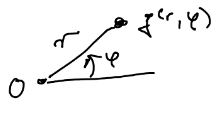
\includegraphics[width=0.2\linewidth]{figures/polarkoordinaten_abbildung}
            \label{fig:polarkoordinaten_abbildung}
        \end{figure}
        und \( f\maps \reals^2\to \reals \).
        \begin{align*}
            \totalderivative+{f\circ g}(r,\phi)&=\totalderivative{f}(g(r,\phi))\matrixmult \totalderivative{g}(r,\phi
            )\\
            \totalderivative{g}(r,\phi)&=\begin{pNiceMatrix} \partial_1 g(r,\phi) & \partial_2 g(r,\phi) \end{pNiceMatrix}=\begin{pNiceMatrix} \Cos{\phi} & -r \Sin{\phi}\\ \Sin{\phi}& r\Cos{\phi} \end{pNiceMatrix}.
        \end{align*}
        Somit 
        \begin{equation*}
            \begin{split}
                \totalderivative+{f\circ g}(r,\phi)&=\begin{pNiceMatrix} \partial_1 f(g(r,\phi)) & \partial_2 f(g(r,\phi))  \end{pNiceMatrix}\matrixmult \begin{pNiceMatrix} \Cos{\phi} & -r\Sin{\phi}\\ \Sin{\phi}& r\Cos{\phi} \end{pNiceMatrix}\\
                &=\transpose-{\begin{pNiceMatrix} \partial_1 f(g(r,\phi))\cdot \Cos{\phi}+\partial_2(f(g(r,\phi)))\cdot\Sin{\phi}\\
                -\partial_1 f(g(r,\phi))\cdot r\Sin{\phi}+\partial_2 f(g(r,\phi))\cdot r \Cos{\phi} \end{pNiceMatrix}}.
            \end{split}
        \end{equation*}
        Man schreibt dafür manchmal
        \begin{align*}
            \partial_r&=\Cos{\phi} \partial_x+\Sin{\phi}\partial_y\\
            \partial_\phi &=-r\Sin{\phi}\partial_x+r\Cos{\phi}\partial_y.
        \end{align*}
    \end{enumerate}
\end{beispiele}
Aber oft ist es \emph{viel} übersichtlicher, die partiellen Ableitungen \emph{nicht} nach den Namen der Variablen zu benennen, sondern durchzunummerieren!
\begin{beispiel*}
    \( f(x,y)=\frac{xy}{x^2+y^2} \) auf \( U=\reals^2\setminus \zeroset \).
    \begin{align*}
        \totalderivative{f}(x,y)=\begin{pNiceMatrix} \frac{y(y^2)-x^2}{(x^2+y^2)}^2 \\ \frac{x(x^2-y^2)}{(x^2+y^2)} \end{pNiceMatrix}\\
        \totalderivative+{f\circ g}(r,\phi)&\begin{aligned}[t]
            &=\frac{1}{r}(\cos^2 \phi-\sin^2 \phi)\begin{pNiceMatrix} \overbrace{-\Sin{\phi}\Cos{\phi}+\Cos{\phi} \Sin{\phi}}^{=0} \\ \underbrace{r\sin^2 \phi+r\cos^2\phi}_{=r} \end{pNiceMatrix}\\
            &=(0,\cos^2\phi -\sin^2\phi).
        \end{aligned}
    \end{align*}
    In diesem Fall rechnet man allerdings schneller direkt:
    \begin{align*}
        \totalderivative+{f\circ g}(r,\phi)=\totalderivative+{\tilde{f}}(r,\phi)=\Cos{\phi}\cdot\Sin{\phi}.
    \end{align*}
\end{beispiel*}
\begin{bemdef}
    Wir hatten allgemeiner gesehen:\\
    Ist \( f\maps U\to \reals^m \), \( U\subset \reals^n \) offen, differenzierbar in \( a \), so gilt
    \begin{align*}
        \partial_v f(a)\cdot \totalderivative{f}(a)\matrixmult v\quad \forall v\in \reals^n.
    \end{align*}
    Ist speziell \( m=1 \), so definiert man
    \begin{align*}
        \grad-{f(a)}\definedas \transpose-{\totalderivative{f}(a)}=\begin{pNiceMatrix} \partial_1 f(a) \\ \Vdots \\ \partial_n f(a) \end{pNiceMatrix}\in \reals^n
    \end{align*}
    \enquote{Gradient von \( f \) in \( a \)}, und schreibt \( \partial_v f(a)=\scalarproduct{\grad-{f(a)}}{v} \).

    Ist \( \grad-{f(a)}\neq 0 \) und \( \norm{v}_{\text{E}}=1 \), so ist
    \begin{equation*}
        \scalarproduct{\grad-{f(a)}}{v}=\norm{\grad-{f(a)}}_{\text{E}}\cdot\Cos{\alpha},
    \end{equation*}
    wobei \( \alpha \) der zwischen \( \grad-{f(a)} \) und \( v \) in \( \reals^n \) eingeschlossene Winkel ist (in der durch die beiden Vektoren aufgespannten Ebene).

    Es folgt: \( \partial_v f(a) \) ist dann am größten, wenn \( v \) in die selbe Richtung zeigt wei \( \grad-{f(a)} \) \timplies der Gradient gibt die Richtung stärksten Anstiegs von \( f \) in \( a \) an.
\end{bemdef}
\begin{beispiel*}
    \( f(x)=x_1^2+x_2^2+2 \).
    \begin{figure}[H]
        \centering
        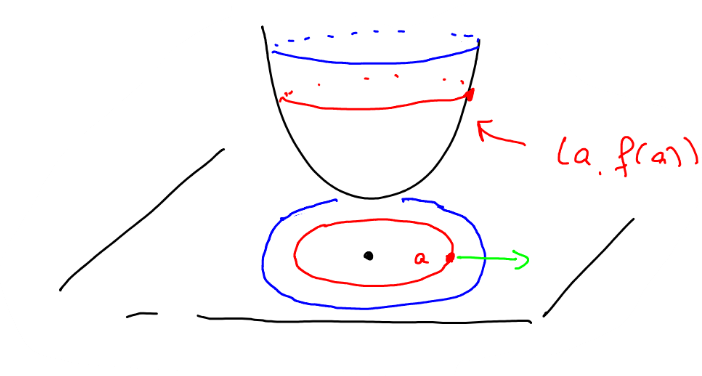
\includegraphics[width=0.5\linewidth]{figures/gradient_beispiel_parabel}
        \label{fig:gradient_beispiel_parabel}
    \end{figure}
\end{beispiel*}
\begin{beispiel*}
    \( f(x)=x^2 \).
    \begin{figure}[H]
        \centering
        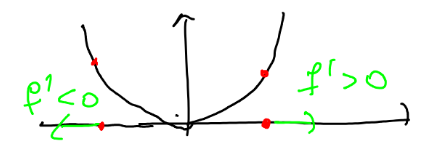
\includegraphics[width=0.4\linewidth]{figures/gradient_beispiel_parabel_2d}
        \caption*{}
        \label{fig:gradient_beispiel_parabel_2d}
    \end{figure}
    Ist \( f \) lediglich \emph{partiell differenzierbar}, \dh  die partiellen Ableitungen existieren auf \( U \), so definiert man dennoch
    \begin{equation*}
        \grad-{f(x)}=\transpose-{(\partial_1 f(x),\dotsc, \partial_n f(x))}
    \end{equation*}
    als den Vektor der partiellen Ableitungen bei \( x \).
\end{beispiel*}
\begin{satz}\label{extremum_notwendige_bedingung}
    Sei \( f\maps U\to \reals \), \( U\subset \reals^n \) offen, \emph{partiell differenzierbar} auf \( U \). Sei \( a\in U \) ein \emph{lokales Maximum} (oder Minimum) von \( f \), \dh  \texists Umgebung \( V \) von \( a \) \sd \( f(x)\leq (a) \) (oder \( f(x)\geq f(a) \) für alle \( x\in V \)). Dann gilt
    \begin{equation*}
        \boxed{\grad-{f(a)}=0}.
    \end{equation*} 
\end{satz}
\begin{proof}
    Betrachte \( g_i(t)\definedas f(a+t e_i) \), \( i=1,\dotsc, n \), mit \( t\in \ointerval{-\varepsilon}{\varepsilon} \) \sd \( B_{\varepsilon}^{\norm{\cdot}}(a)\subset U \).
    \begin{figure}[H]
        \centering
        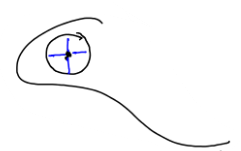
\includegraphics[width=0.5\linewidth]{figures/extrema_notwendige_bedingung_beweis_umgebung}
        \label{fig:extrema_notwendige_bedingung_beweis_umgebung}
    \end{figure}
    Ist \( a \) lokales Extremum (also lokales Maximum oder Minimum) von \( f\), so ist \( t=0 \) lokales Extremum von \( g_i \). Die \( g_i \) sind in \( t=0 \) differenzierbar, denn
    \begin{equation*}
        g_i'(0)=\partial_i f(a)\quad (\text{Definition Richtungsableitung})
    \end{equation*}
    \diffcourse{1} \timplies \( g_i'(0)=0 \) \timplies \Beh.
\end{proof}
\begin{beispiele*}
    \begin{enumerate}
        \item \( f(x)=x_1^2+x_2^2+2 \). Außer in \( a=0 \) kann kein Extremum vorliegen.
        \item \( f(x,y)=\begin{cases}
            \frac{xy}{x^2+y^2}&(x,y)\neq (0,0)\\
            0 &(x,y)=(0,0).
        \end{cases} \). \( \partial_1 f(0)=0=\partial_2 f(0) \), also könnte \( 0 \) ein Extremum sein. Ist es aber nicht, da für \( x=y=\varepsilon>0 \) gilt \( f(\varepsilon,\varepsilon)=\frac{1}{2}>0 \) und für \( -x=y=\varepsilon>0 \). \( f(-\varepsilon,\varepsilon)=-\frac{1}{2}<0 \).
    \end{enumerate}
\end{beispiele*}
\begin{bemerkung*}
    Hinreichende Kriterien für das Vorliegen lokaler Extremstellen werden wir erst später kennen lernen. Wie in der \diffcourse{1} benötigen wir dafür die 2.\ Ableitung.
\end{bemerkung*}
\begin{satz}\label{stetige_partielle_zu_ableitung}
     Sei \( f\maps U\to \reals \), \( U\subset \reals^n \) offen. Existieren alle partiellen Ableitungen \( \partial_j f(x) \) für alle \( x\in U \), \emph{und} sind sie stetig in \( a\in U \), so ist \( f \) in \( a \) differenzierbar.
\end{satz}
\begin{proof}
    Wir wählen ein Norm \( \norm{\cdot} \) auf \( \reals^n \). \( U \) offen \timplies \texists \( \delta>0 \) \sd  \( B_{\delta}^{\norm{\cdot}}(a)\subset U \). Sei \( h\in B_{\delta}^{\norm{\cdot}}(0) \), also \( a+h\in B_{\delta}^{\norm{\cdot}}(a) \). Setze
    \begin{equation*}
        x^{(j)}\definedas a+\sum_{i=1}^{j} h_i e_i \in \reals^n\quad j=0,\dotsc,n,
    \end{equation*}
    also \( x^{(0)}=a \), \( x^{(1)}=(a_1+h_1,a_2,\dotsc, a_n),\dotsc, x^{(n)}=a+h \). Es ist \( x^{(j)}-x^{(j-1)}=(0,\dotsc,0,h_j,0,\dotsc,0) \) \timplies (MWS, \diffcourse{1}) \texists \( \eta_j\in \interval{0}{1} \) \sd 
    \begin{align*}
        &f(x)=\partial_j f(\underbrace{x_1^{(j-1)},\dotsc,x_{j-1}^{(j-1)},x_j^{(j-1)}+\eta_j h_j,a_{j+1}, \dotsc, a_n}_{x^{j-1}+\eta_j h_j e_j\defines y^{(j)}})\cdot h_j\\
        \implies &f(a+h)-f(a)\begin{aligned}[t]
            &=\sum_{j=1}^{n}(f(x^{(j)})-f(x^{(j-1)}))\\
            &=\sum_{j=1}^{n}\partial_j f(y^{(j)}) h_j\\
            &\needed{=} \begin{pNiceMatrix} \partial_1 f(a) & \Cdots & \partial_n f(a) \end{pNiceMatrix}\begin{pNiceMatrix} h_1 \\ \Vdots \\ h_n \end{pNiceMatrix}+ \underline{R}_a(h)
        \end{aligned}
    \end{align*}
    also ist
    \begin{align*}
        &\underline{R}_a(h)=\sum_{j=1}^{n} (\partial_j f(y^{(j)})-A_j)h_j\quad A=\partial_j f(a)\\
        \overset{\text{CS}}{\implies}&\frac{\abs{\underline{R}_a(h)}}{\norm{h}}\leq C\norm{(\partial_1 f(y^{(1)})-A_1,\dotsc,\partial_n f(y^{(n)})-A_n)}_{\text{E}}\goesto 0 \quad h\goesto 0,
    \end{align*}
    denn \( \lim_{h\goesto 0}y^{(j)}=\lim_{h\goesto 0}x^{(j-1)}+\eta_j h_j e_j=a \) (in \( \reals^n \)) und die \( \partial_j f \) sind in \( a \) stetig nach Voraussetzung, \sd
    \begin{align*}
        \lim_{h \goesto 0}\partial_j f(y^{(j)})=(\partial_j f)(\lim y^{(j)})=\partial_j f(a).
    \end{align*}
\end{proof}
\begin{bemerkungen}
    \begin{enumerate}
        \item \label{stetig_differenzierbar} Man sieht: Sind die \( \partial_j  \) auf \( U \) stetig, so ist auch die Ableitung \( x\mapsto \totalderivative{f}(x) \) eine stetige Abbildung \( U\to \Mat(m\times n, \reals) \). Man sagt in dem Fall: \( f \) ist \emph{stetig differenzierbar}.
        \item \label{stetige_partielle_zu_ableitung:nicht_nur_reell} Die Einschränkung auf reellwertige Funktionen ist keine, denn: \( f\maps U\to \reals^m \) ist genau dann in \( a\in U\subset \reals^n \) differenzierbar, wenn alle Komponentenfunktionen \( f_j\maps U\to \reals \) differenzierbar sind (\( j=1,\dotsc, m \))-
    \end{enumerate}
\end{bemerkungen}
\begin{proof}
    \begin{proofdescription}
        \item[\ref{stetige_partielle_zu_ableitung:nicht_nur_reell}] \( f(a+h)=f(a)+A\matrixmult h+\underline{R}(h) \), \( A_{ji}=\partial_j f_j(a) \) 
        \begin{equation*}
            \iff f_j(a+h)=f_(a)+\begin{pNiceMatrix} \partial_1 f_j(a) & \Cdots & \partial_n f_j(a) \end{pNiceMatrix}\matrixmult h+\underline{R}_j(h)\quad \forall j=1,\dotsc, m
        \end{equation*}
        und
        \begin{equation*}
            \frac{\underline{R}(h)}{\norm{h}}\goesto 0 \text{ in }\reals^m\iff \frac{\explicitnorm{\max}{\underline{R}(h)}}{\norm{h}}\goesto 0\iff \frac{\abs{R}_j(h)}{\norm{h}}\goesto 0\quad j=1,\dotsc,m.
        \end{equation*}
        \item[\ref{stetig_differenzierbar}] Dito: \( U\to \Mat(m\times n,\reals) \) ist stetig \tiff alle Komponentenfunktionen \( A_{ij}\maps U\to \reals \) sind stetig.
    \end{proofdescription}
    
\end{proof}
\begin{bemerkung*}
    Stetig differenzierbar \timplies differenzierbar \timplies partiell differenzierbar.

    Die Umkehrungen sind im Allgemeinen falsch.
\end{bemerkung*}
\begin{bemerkung*}[Erinnerung (\diffcourse{1}) MWS]
    \( f\maps I\to \reals \) differenzierbar, \( I \) Intervall, \texists \( \epsilon\in \interval{0}{1} \) \sd
    \begin{equation*}
        f(a+h)-f(a)=f'(a+\eta h)\cdot h.
    \end{equation*}
    Ist \( f \) stetig differenzierbar, folgt aus dem Hauptsatz der Differenzial- und Integralrechnung eine andere Variante:
    \begin{equation*}
        f(a+h)-f(a)=\Integrate{f'(u)}{u,a,a+h}=\Integrate{f'(a+th)}{t,0,1}\cdot h.
    \end{equation*}
\end{bemerkung*}
Eine analoge Aussage wollen wir nun im \( \reals^n \) beweisen.
\begin{definition*}\index{Integral}
    Sei \( A\maps I\to \reals^k \),\( I\subset \reals \) Intervall, stetig. Dann ist das \emph{Integral von \( A \)} über \( \interval{a}{b}\in I \) definiert als
    \begin{equation*}
        \Integrate{A(t)}{t,a,b}=\begin{pNiceMatrix} \Integrate{A_1(t)}{t,a,b} \\ \Vdots \\ \Integrate{A_k(t)}{t,a,b} \end{pNiceMatrix}.
    \end{equation*}
    Insbesondere ist das Integral einer matrixwertigen, stetigen Funktion \( A\maps I\to \Mat(m\times n,\reals) \) die Matrix, deren Einträge gleich den Integralen der Komponenten von \( A(t) \) ist, also
    \begin{equation*}
        \Integrate{A(t)}{t,a,b}=\p*{ \Integrate{A_{ij}(t)}{t,a,b} }_{\substack{1\leq i\leq m\\1\leq j\leq n}}.
    \end{equation*}
\end{definition*}
\begin{satz}\label{verbindungsstrecke_integral_mws}
    Sei \( f\maps U\to \reals^m \), \( U\subset \reals^n \), stetig differenzierbar. Sei \( a\in U \) und \( h\in \reals^n \) \sd  die Verbindungsstrecke
    \begin{equation*}
        \Set{a+th|t\in \interval{0}{1}}\subset U.
    \end{equation*}
    Dann gilt:
    \begin{equation*}
        f(a+h)-f(a)=\p*{ \Integrate{\totalderivative{f}(a+th)}{t,0,1} }\matrixmult h.
    \end{equation*}
    \begin{figure}[H]
        \centering
        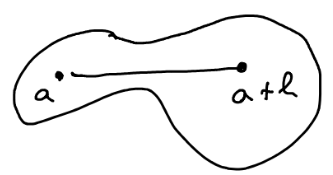
\includegraphics[width=0.5\linewidth]{figures/mws_integral_verbindungsstrecke}
        \label{fig:mws_integral_verbindungsstrecke}
    \end{figure}
\end{satz}
\begin{proof}
    Wir arbeiten zeilenweise, betrachten also die Komponentenfunktionen. Setze \( g_i(t)\definedas f_i(a+th) \). Dann ist \( g_i \) stetig differenzierbar, denn mit der Kettenregel gilt \( g_i'(t)=\totalderivative{f}_i(a+th)\matrixmult h \).
    \begin{equation*}
        \begin{split}
            f_i(a+h)-f_i(a)&=g_i(1)-g_i(0)\\
            &=\Integrate{g_i'(t)}{t,0,1}\\
            &=\Integrate{\totalderivative{f}_i(a+th)\matrixmult h}{t,0,1}\\
            &\explain[big]{\int \text{ linear}}{=}\underbrace{\p*{ \Integrate{\totalderivative{f}_i(a+th)}{t,0,1} }}_{(1\times n)\text{-Matrix}}\matrixmult h\quad 1\leq i \leq m.
        \end{split}
    \end{equation*}
    Dies sind die Zeilen der Matrix \( \Integrate{\totalderivative{f}(a+th)}{t,0,1} \).
\end{proof}
\begin{folgerung}\label{differenz_abschaetzung_ableitung_verbindungsstrecke}
    Unter den Voraussetzungen von \ref{verbindungsstrecke_integral_mws} gilt \( \norm{f(x+h)-f(x)}_{\text{E}}\leq C\norm{h} \) mit
    \begin{equation*}
        C=\sup_{t\in \interval{0}{1}}\norm{\totalderivative{f}(x+th)}_{\text{op}}.
    \end{equation*}
\end{folgerung}
Der Beweis benötigt noch ein Lemma:
\begin{lemma}\label{integral_norm_dreiecksungleichung}
    Sei \( v\maps \interval{a}{b}\to \reals^m \) stetig. Dann gilt
    \begin{equation*}
        \norm{\Integrate{v(t)}{t,a,b}}_{\text{E}}\leq \Integrate{\norm{v(t)}_{\text{E}}}{t,a,b}.
    \end{equation*}
\end{lemma}
\begin{proof}
    Sei \( \reals^m\ni u=\Integrate{v(t)}{t,a,b} \). Dann gilt
    \begin{equation*}
        \begin{split}
            \norm{n}_{\text{E}}^2&=\scalarproduct{u}{u}\\
            &=\scalarproduct{\Integrate{v(t)}{t,a,b}}{u}\\
            &\explain[big]{\text{Linearität}}{=}\Integrate{\scalarproduct{v(t)}{u}}{t,a,b}\\
            &\explain{\text{Monotonie und C-S}}{\leq}\Integrate{\norm{v(t)}_{\text{E}}\norm{u}_{\text{E}}}{t,a,b}\\
            &=\norm{u}_{\text{E}} \Integrate{\norm{v(t)}_{\text{E}}}{t,a,b}.
        \end{split}
    \end{equation*}
\end{proof}
\begin{bemerkungen*}
    \begin{enumerate}
        \item Wegen der Äquivalenz aller Normen auf \( \reals^n \) gilt diese Abschätzung ebenso wie \thref{differenz_abschaetzung_ableitung_verbindungsstrecke} auch für beliebige Normen auf \( \reals^n \):
        \begin{equation*}
            \begin{split}
                \norm{\Integrate{v(t)}{t}}&\leq C_1\norm{\Integrate{v(t)}{t}}_{\text{E}}\\
                &\leq C_1\Integrate{\norm{v(t)}_{\text{E}}}{t}\\
                &\leq C_1 C_2 \Integrate{\norm{v(t)}}{t}.
            \end{split}
        \end{equation*}
        \item Es folgt, dass für
        \begin{equation*}
            X=(\explain{\sup\norm{v(t)}<\infty \text{, da \( \interval{a}{b} \) kompakt und \( v \) stetig.}}{\stetigefunktionen}(\interval{a}{b},\reals^k),\supnorm{\cdot}),
        \end{equation*}
        \( \int_a^b\maps X\to \reals^k \) stetig ist, denn \( \int_a^b \) ist linear und
        \begin{equation*}
            \begin{split}
                \norm{\int_a^b}_{\text{op}}&=\sup_{0\neq v \in \stetigefunktionen}\quot{\norm{\Integrate{v(t)}{t,a,b}}}{\supnorm{v}}\\
                &\leq C\sup_{v\neq 0}\quot{\norm{\Integrate{v(t)}{t,a,b}}_{\text{E}}}{\supnorm{v}}\\
                &\leq C\sup_{v\neq 0}\quot{\Integrate{\norm{v(t)}_{\text{E}}}{t,a,b}}{\supnorm{v}}\\
                &\leq \tilde{C}(b-a),
            \end{split}
        \end{equation*}
        denn \( \norm{v(t)}_{\text{E}}\leq \sup_{t}\norm{v(t)}_\text{E}\leq C_0\sup_t\norm{v(t)}=C_0\supnorm{v} \).
    \end{enumerate}
\end{bemerkungen*}
\begin{proof}[Beweis von \thref{differenz_abschaetzung_ableitung_verbindungsstrecke}]
    \begin{equation*}
        \begin{split}
            \norm{f(x+h)-f(x)}_{\text{E}}&\leq \Integrate{\norm{\totalderivative{f}(x+th)\matrixmult h}_{\text{E}}}{t,0,1}\\
            &\leq \Integrate{\norm{\totalderivative{f}(x+th)}_{\text{op}}\matrixmult \norm{h}_{\text{E}}}{t,0,1}.
        \end{split}
    \end{equation*}
    Das Supremum wird angenommen, da \( t\mapsto \norm{\totalderivative{f}(x+th)}_{\text{op}} \) stetig ist und \( \interval{0}{1} \) kompakt.
\end{proof}
\section{Implizite Funktionen} Eine Anwendung der Kettenregel

Manchmal ist es einfacher, eine \( 1 \)-dimensionale Ableitung über eine Ableitung einer höherdimensionalen Funktion zu berechnen. Betrachte etwa zwei differenzierbare Funktionen \( f\maps U\to \reals \), \( U\subset \reals^2 \) offen, und \( g\maps I\to \reals \). Sei \( \Gamma_g\subset U \) und es gelte
\begin{equation*}
    f(\underbrace{t,g(t)}_{\in \Gamma_g})=0\quad \forall t\in I.
\end{equation*}
Dann gilt (Kettenregel!) (mit \( \Id(t)=t \)):
\begin{equation*}
    \begin{split}
        0&=D*{f\circ \begin{pNiceMatrix} \Id \\ g \end{pNiceMatrix}}(t)\\
         &=\totalderivative{f}\p*{ (t,g(t)) }\matrixmult \totalderivative{\begin{pNiceMatrix} \Id \\ g \end{pNiceMatrix}}(t)\\
         &=\begin{pNiceMatrix} \partial_1 f(t,g(t)) & \partial_2 f(t,g(t)) \end{pNiceMatrix}\matrixmult \begin{pNiceMatrix} 1 \\ g'(t) \end{pNiceMatrix}
    \end{split}
\end{equation*}
\timplies Ist \(  \partial_2 f(t,g(t))\neq 0 \), so gilt
\begin{align*}
    g'(t)=-\frac{\partial_1 f(t,g(t))}{\partial_2 g(t,g(t))}.
\end{align*}
\begin{beispiel*}
    \( g\maps \ointerval{0}{1}\to \reals \), \( g(t)=\ArcSin{\sqrt{1-t^3}} \), also \( \Sin{g(t)}=\sqrt{1-t^3} \), also \( (\Sin{g(t)})^2=1-t^3 \). Also gilt \( f(t,g(t))=0 \) für
    \begin{align*}
        f(x,y)&=(\Sin{y})^2-1+x^3\\
        \totalderivative{f}(x,y)&=(3x^2,2\Sin{y} \Cos{y})\\
        \implies g'(t)&\begin{aligned}[t]
            &=-\frac{3t^2}{2\Sin{g(t)}\underbrace{\Cos+{g(t)}}_{>0,}}
            \intertext{da \( t\in \ointerval{0}{1} \) und \( \sqrt{1-t^3}\in \ointerval{0}{1} \), somit \( g(t)\in \ointerval{0}{\quot{\pi}{2}} \) \timplies \( \Cos{g(t)}=+\sqrt{1-\underbrace{\sin^2 g(t)}_{1-t^3}}=\sqrt{t^3} \)}
            &=-\frac{3t^2}{2\sqrt{1-t^3}\sqrt{t^3}}.
        \end{aligned}
    \end{align*}
\end{beispiel*}
% !TEX root = ./Vorlesungsmitschrift DIFF 2.tex  
\lecture{Do 14.05. 10:15}{}
\begin{satz}\label{funktion_ableiten_mit_hoeheren_abbildungen}
  Sei \( f\maps \underrelate{\vertrelation{\supset}}{\reals^k}{B_{r_1}^{\norm{\cdot}}(a)}\times \underrelate{\vertrelation{\supset}}{\reals^m}{B_{r_2}^{\norm{\cdot}}(b)}\to \reals^m \) eine Abbildung mit \( f(a,b)=0 \), die in \( (a,b) \) differenzierbar sei. Sei zudem \( D_2 f(a,b) \), definiert über
  \begin{equation*}
    \totalderivative{f}(a,b)=(\underbrace{\partial_1 f(a,b)\, \cdots\,  \partial_k f(a,b)}_{\defines D_1 f(a,b)\in \Mat(m\times k)}\, \underbrace{\partial_{k+1}f(a,b)\, \cdots\, \partial_{k+m}f(a,b)}_{\defines D_2 f(a,b)\in \Mat(m\times m)}),
  \end{equation*}
  invertierbar. Sei zudem \( g\maps B_{r_1}(a)\to \reals^m \) stetig und gelte \( g(B_{r_1}(a))\subset B_{r_2}(b) \) und \( g(a)=b \) und \( f(x,g(x))=0 \) \tforall \( x\in B_{r_1}(a) \). Dann ist \( g \) in \( a \) differenzierbar und es gilt
  \begin{equation*}
    \totalderivative{g}(a)=-\inverse{\p*{ D_2f(a,b) }}D_1 f(a,b)\in \Mat(m\times k, \reals).
  \end{equation*}
\end{satz}
\begin{proof}
  Es gilt für \( h=(h_1,h_2)\in B_{r_1}(0)\times B_{r_2}(0) \)
  \begin{equation*}
    f(\underbrace{(a,b)+h}_{=(a+h_1,b+h_2)})=0+D_1f(a,b)\matrixmult h_1+D_2 f(a,b)\matrixmult h_2+\underline{R}_{(a,b)}(h)
  \end{equation*}
  mit \( \frac{\underline{R}_{(a,b)}(h)}{\norm{h}}\goesto 0 \) \tforall \( x\in B_{r_1}(a) \) folgt
  \begin{equation*}
    \begin{split}
      0=f(\underbrace{a+h_1}_{\in B_{r_1}(a)},g(a+h_1))=&D_1 f(a,b)\matrixmult h_1\\
      &+D_2 f(a,b)\matrixmult (g(a+h_1)-b)\\
      &+\underline{R}_{(a,b)}(h_1,g(a+h_1)-b)\quad \forall h_1\in B_{r_1}(0).
    \end{split}
  \end{equation*}
  Also
  \begin{equation*}
    \begin{split}
      g(a+h_1)=&g(a)-\inverse{D_2f(a,b)}\matrixmult D_1 f(a,b)\matrixmult h_1\\
      &\underbrace{-\inverse{D_2f(a,b)}\matrixmult \underline{R}_{(a,b)}(h_1,g(a+h_1)-b)}_{\defines \tilde{R_{a,b}^g(h_1)}}\quad \forall h_1\in B_{r_1}(0).
    \end{split}
  \end{equation*}
  Wir sind fertig, wenn wir zeigen können, dass
  \begin{equation*}
    \frac{\tilde{R}_{a,b}^g(h_1)}{\norm{h_1}}\goesto 0 \text{ für }h_1\goesto 0.
  \end{equation*}
  Wegen der Differenzierbarkeit von \( f \) in \( (a,b) \) \texists  \( \tilde{C} \) und \( \delta_1,\delta_2>0 \), \( \delta_i<r_i \), \sd
  \begin{equation*}
    \norm{\underline{R}_{(a,b)}(h_1,h_2)}\leq \tilde{C}(\norm{h_1}+\norm{h_2})\quad \forall h_1\in B_{\delta_1}(0), h_2\in B_{\delta_2}(0),
  \end{equation*}
  also
  \begin{equation*}
    \norm{\underline{R}_{(a,b)}(h_1,g(a+h_1)-b)}\leq \tilde{C}(\norm{h_1}+\norm{g(a+h_1)-b})
  \end{equation*}
  für alle \( h_1 \) \sd \( \norm{h_1}<\delta_1 \) und \( \norm{g(a+h_1)-b}<\delta_2 \). Wegen der Stetigkeit von \( g \) in \( a \) gibt es \( \delta>0 \),\( \delta<\delta_1 \), \( \norm{g(a+h_1)-\underbrace{g(a)}_{=b}}<\delta_2 \) für alle \( h_1\in B_{\delta}(0) \).
\end{proof}
\begin{bemerkungen*}
  \begin{enumerate}
    \item Ist \( f,g \) wie in \thref{funktion_ableiten_mit_hoeheren_abbildungen} und \( f \) überall \emph{stetig} differenzierbar. Ist dann \( D_2 f(a,b) \) invertierbar. So gibt es eine Umgebung \( V_1\times V_2 \) von \( (a,b) \) \sd \( D_2f(x,y) \) invertiertbar ist für alle \( (x,y)\in V_1\times V_2 \) (denn \( (x,y)\mapsto \Det D_2f(x,y) \) ist stetig, da es ein Polynom stetiger Funktionen ist und \( \Det D_2 f(a,b)\neq 0 \)).
    \item Das Beispiel vom letzten Mal ist genau von diesem Typ.
  \end{enumerate}
\end{bemerkungen*}
Umgekehrt kann man eine Funktion \( g \) wie oben durch \enquote{Auflösen der Gleichung \( f(x,g(x))=0 \)} bestimmen (unter gewissen Voraussetzungen):
\begin{satz}[Satz von der impliziten Funktion]\label{satz_von_der_impliziten_funktion}\index{Satz von der impliziten Funktion}
  Seien \( U_1\subset \reals^k \), \( U_2\subset \reals^m \) offen und \( f\maps U_1\times U_2\to \reals^m \) stetig differenzierbar. Sei \( (a,b) \in U_1\times U_2 \) \sd \( f(a,b)=0 \) und \( D_2f(a,b)\in \Mat(m \times m,\reals) \) invertierbar. Dann gibt es offene Umgebungen \( V_1\subset U_1 \), \( V_2\subset U_2 \) von \( a \) \bzw \( b \) und eine stetige Funktion \( g\maps V_1\to \reals^m \), \( g(V_1)\subset V_2 \), \sd \( f(x,g(x))=0 \) \tforall  \( x\in V_1 \). Ist \( (x,y)\in V_1\times V_2 \) \sd \( f(x,y)=0 \), so ist \( y=g(x) \).
\end{satz}
\begin{bemerkungen*}
  \begin{enumerate}
    \item \label{implizite_funktion_auf_umgebung_stetig_differenzierbar} Aus \ref{funktion_ableiten_mit_hoeheren_abbildungen} und der folgenden Bemerkung folgt, dass \( g \) in einer eventuell verkleinerten Umgebung \( \tilde{V_1}\subset V_1 \) von \( a \) sogar stetig differenzierbar ist und gilt
    \begin{equation*}
      \totalderivative{g}(x)=-\inverse{D_2 f(x,g(x))}\matrixmult D_1f(x,g(x))\quad \forall x\in \tilde{V_1}
    \end{equation*}
    \item Für den Satz ist wichtig, dass \( U_1\times U_2 \) gegebenenfalls verkleinert wird:
    \begin{figure}[H]
      \centering
      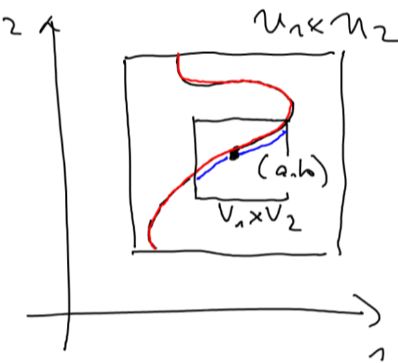
\includegraphics[width=0.5\linewidth]{figures/verkleinerter_definitionsbereich_implizite_funktion}
      \caption*{\textcolor{Blue}{\( \Gamma_g=\Set{(x,g(x))|x\in V_1} \)},\textcolor{Red}{}}
      \label{fig:verkleinerter_definitionsbereich_implizite_funktion}
    \end{figure}
    Betrachtete man auch den oberenTeil der Kurve,könnte man \( x \) nicht ein eindeutiges \( y \) zuordnen.
    \item Die Einschränkung auf Definitionsbeiche der Form \( U_1\times U_2  \) ist keine, sie vereinfacht nur die Notation. Ist \( f \) auf \( U\subset \reals^{k+m} \) offen, findet man stets \( U_1\subset \reals^k \), \( U_2\subset \reals^m \) \sd \( U_1\times U_2\subset U \).
    \item Die Einschränkung auf \( N_f(0) \) ist keine: Will man etwa die Gleichung \( f(x,y)=c \) auflösen, wendet man des Satz auf \( \tilde{f} \) an mit \( \tilde{f}(x,y)=f(x,y)-c \).
    \item Durch Umnummerierung kann man auch andere \( m\times m \)-Untermatrizen von \( \totalderivative{f} \) betrachten als die letzten \( m \).
    \item Unter den Voraussetzungen von \ref{satz_von_der_impliziten_funktion} sagt man: \( g \) ist durch \( f(x,y)=0 \) \emph{implizit} gegeben und man \emph{löst} \( f(x,y)=0 \) \emph{nach \( y \) auf}.
  \end{enumerate}
\end{bemerkungen*}
\begin{beispiele*}
  \begin{enumerate}
    \item \( f(x,y)=3y-x^2+1 \) auf \( \reals^2 \). \( \totalderivative{f}(a,b)=\begin{pNiceMatrix} -2a & 3 \end{pNiceMatrix} \), \( 3\neq 0 \) ist invertierbar, \ref{satz_von_der_impliziten_funktion} \timplies \texists  \( g\maps I\to \reals \) \sd \( f(x,g(x))=0 \)\tforall \( x\in I \). In diesem Fall sogar \( I=\reals \): \( g(x)=\frac{1}{3}(x^2-1) \).
    \begin{figure}[H]
      \centering
      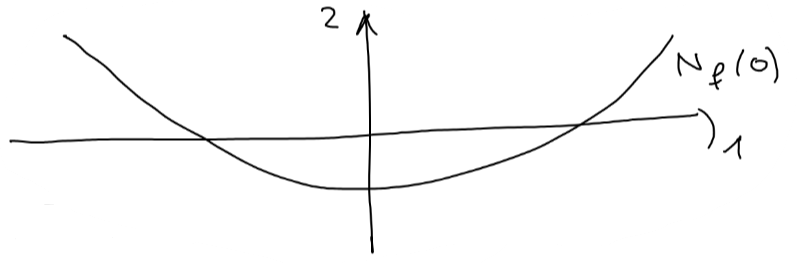
\includegraphics[width=0.5\linewidth]{figures/implizite_funktion_beispiel_kein_eingeschraenkter_definitionsbereich}
      \label{fig:implizite_funktion_beispiel_kein_eingeschraenkter_definitionsbereich}
    \end{figure}
    \item \( f(x,y)=3x-y^2+1 \) auf \( \reals^2 \). \( \totalderivative{f}(a,b)=\begin{pNiceMatrix} 3 & -2b \end{pNiceMatrix} \). \ref{satz_von_der_impliziten_funktion} \timplies Zu \( b\neq 0 \) gibt es \( g\maps I\to \reals \). \( b>0 \): \( g(x)=+\sqrt{3x+1} \), \( x>-\frac{1}{3} \). \( b<0 \): \( g(x)=-\sqrt{3x+1} \).
    \begin{figure}[H]
      \centering
      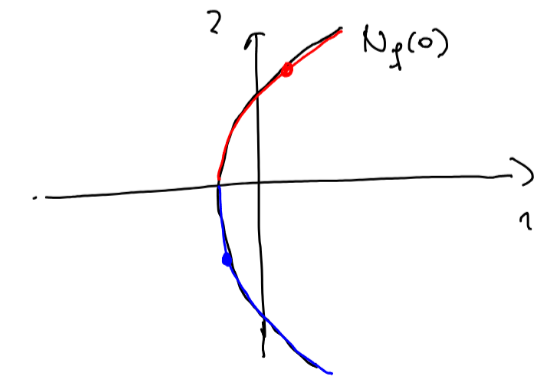
\includegraphics[width=0.5\linewidth]{figures/implizite_funktion_beispiel_eingeschraenkter_definitionsbereich}
      \caption*{\( f(x,g(x))=0 \)}
      \label{fig:implizite_funktion_beispiel_eingeschraenkter_definitionsbereich}
    \end{figure}
  \end{enumerate}
\end{beispiele*}
\begin{proof}[Beweis von \thref{satz_von_der_impliziten_funktion}]
  \begin{proofenumerate}[label=\rechtsklammer{\arabic*}]
    Setze \( B\definedas D_2f(a,b)\) und definiere eine Abbildung \( h\maps U_1\times U_2\to \reals^m \) vermöge
    \begin{equation*}
      h(x,y)=y-b-\inverse{B} f(x,y).
    \end{equation*}
    Dann gilt 
    \begin{equation*}
      D_2 h(x,y)=\mathds{1}-\inverse{B} D_2 f(x,y).
    \end{equation*}
    \timplies \( D_2 h(a,b)=0 \) \timplies (da alle Ableitungen stetig sind) \texists \( W_1\subset U_1 \), \( W_2\subset U_2 \) offene Umgebungen von \( a \) \bzw \( b \) \sd
    \begin{equation*}
    \norm{D_2 h(x,y)}\leq \frac{1}{2}\quad \forall x\in W_1,\logicspace y\in W_2\tag{\(*\)}.\label{satz_von_der_impliziten_funktion:beweis:h:ableitungsnorm_bschraenkt}
    \end{equation*}
    Wähle \( r>0 \) \sd \( V_2\definedas B_r^{\norm{\cdot}}(b)\subset W_2 \). Es ist \( h(a,b)=0 \) \timplies (da \( h \) differenzierbar ist und somit auch stetig) \texists offene Umgebung \( V_1\subset W_1 \) von \( a \) \sd 
    \begin{equation*}
      \varepsilon\definedas \sup_{x\in V_1}\norm{h(x,b)}<\frac{r}{2} \tag{\( ** \)}\label{satz_von_der_impliziten_funktion:beweis:h:norm_beschraenkt}
    \end{equation*}
    (auf einem Kompaktum \( \subset W_1 \) um \( a \) ist \( x\mapsto h(x,b) \) beschränkt und wird auf einem hinreichend kleinen Kompaktum beliebig klein. Um \( V_1 \) offen zu erhalten, nehmen wir das Innere eines solchen Kompaktums).
    \item Wir zeigen jetzt: Zu jedem \( x\in V_1 \) gibt es höchstens ein \( y\in V_2 \) \sd \( f(x,y)=0 \) also \sd \( h(x,y)=y-b \).
    
    Sei also \( x\in V_1 \) und seien \( y_1 \) und \( y_2 \) \sd \( h(x,y_1)=y_1-b \) und \( h(x,y_2)=y_2-b \).
    \begin{align*}
      \implies &y_1-y_2=h(x,y_1)-h(x,y_2)\\
      \underset{\mathclap{\text{MWS und \eqref{satz_von_der_impliziten_funktion:beweis:h:ableitungsnorm_bschraenkt}}}}{\implies}&\norm{y_1-y_2}\begin{aligned}[t]
        &=\norm{h(x,y_1)-h(x,y_2)}\\
        &\explain{\text{\( \zeta \) auf der Verbindungsstrecke zw.\ \( y_1 \) und \( y_2 \) (liegt in \( V_2=B_r(b) \))}}{=}\norm{D_2 h(x,\zeta)}\matrixmult\norm{y_1-y_2}\\
        &\leq \frac{1}{2}\norm{y_1-y_2}
      \end{aligned}\\
      \implies &\norm{y_1-y_2}=0 \implies y_1=y_2.
    \end{align*}
    \item Wir zeigen nun die Existent einer Funktion \( g \) wie im Satz behauptet. Setze dazu \( g_0(x)=b \) und definiere rekursiv für \( x\in V_1 \):
    \begin{equation*}
      g_{j+1}(x)\definedas b+h(x,g_j(x)).
    \end{equation*}
    \begin{proofenumerate}[label=\rechtsklammer{\alph*}]
      \item Es gilt
      \begin{equation*}
        \norm{g_{j+1}-g_j}_{\infty, V_1}\leq 2^{-j}\explain{\text{aus \eqref{satz_von_der_impliziten_funktion:beweis:h:norm_beschraenkt}}}{\varepsilon}.
      \end{equation*}
      Induktionsanfang: 
      \begin{equation*}
        \norm{g_1-g_0}_{\infty,V_1}=\norm{h(x,b)}_{\infty, V_1}=\varepsilon.
      \end{equation*}
      Induktionsschritt: Sei die Behauptung für \( i\leq n \) bewiesen. 
      \begin{align*}
        &g_{n+2}(x)-g_{n+1}(x)=h(x,g_{n+1}(x))-h(x,g_n(x)).\\
        \underset{\mathclap{\text{MWS und \eqref{satz_von_der_impliziten_funktion:beweis:h:ableitungsnorm_bschraenkt}}}}{\implies}&\norm{g_{n+2}-g_{n+1}}_{\infty,V_1}\leq \frac{1}{2}\norm{g_{n+1}-g_n}_{\infty,V_1}.
      \end{align*}
      \begin{bemerkung*}
        Der MWS darf tatsächlich angewendet werden. \( g_{n+1}(x), g_n(x) \) und somit auch die Verbindungsstrecke zwischen ihnen liegen in \( V_2 \), denn nach Induktionsvoraussetzung gilt für alle \( j\leq n \)
        \begin{equation*}
          \norm{g_{j+1}-b}_{\infty,V_1}\leq \sum_{i=0}^{j}\norm{g_{i+1}-g_i}\leq 2\varepsilon<r
        \end{equation*}
        (da \( g_{j+1}-b=\sum_{i=0}^{j}(g_{i+1}-g_i) \) ist). Somit darf der MWS auf
        \begin{equation*}
          h(x,g_{n+1}(x))-h(x,g_n(x))
        \end{equation*}
        angewendet werden.
      \end{bemerkung*}
      \item Es folgt \( \norm{g_n-b}_{\infty, V_1}<r \) und somit \( g_n(V_1)\subset V_2 \). Denn
      \begin{align*}
        &g_n=\sum_{j=0}^{n-1} (g_{j+1}-g_j)+b\quad (\text{Teleskopsumme})
        \implies &\norm{g_n-b}_{\infty,V_1}\leq \sum_{j=0}^{n-1}2^{-j}\varepsilon \explain{\text{geom.\ Reihe}}{\leq}2\varepsilon<r.
      \end{align*}
      \item Zudem gilt: \( \norm{\sum_{j=0}^{\infty}(g_{j+1}-g_j)}_{\infty,V_1} \) hat die Majorante \( \sum_{j=0}^{\infty}2^{-j}\varepsilon \). \timplies Die Reihe konvergiert gleichmäßig auf \( V_1 \) \timplies (\diffcourse{1})
      \begin{equation*}
        g\definedas \lim_{n \goesto \infty} g_n=\sum_{j=0}^{\infty}(g_{j+1}-g_j)+b
      \end{equation*}
      ist stetig auf \( V_1 \) und
      \begin{equation*}
        \norm{g-b}_{\infty,V_1}\leq 2\varepsilon<r,
      \end{equation*}
      also \( g(V_1)\subset V_2 \).
    \end{proofenumerate}
    Aus der Definition folgt durch Grenzübergang auf beiden Seiten (\( h \) ist stetig)
    \begin{equation*}
      g(x)=b+h(x,g(x))\quad \forall x\in V_1,
    \end{equation*}
    also \( g(x)=g(x)-\inverse{B}f(x,g(x)) \), also
    \begin{equation*}
      f(x,g(x))=0\quad \forall x\in V_1.
    \end{equation*}
  \end{proofenumerate}
\end{proof}
\begin{folgerung}\label{satz_von_der_impliziten_funktion:hoehenlinie_folgerung}
  Sei \( f\maps U\to \reals \), \( U\subset \reals^2 \) offen, stetig differenzierbar und sei \( \ointerval{a}{b}\in U \), \( f(a,b)=c \) und \( \grad-{f(a,b)}\neq 0 \). Dann kann man ein Stück der Höhenlinie \( N_f(c) \) als Graph einer Funktion beschreiben. Denn sei \( \partial_2 f(a,b)\neq 0 \), \thref{satz_von_der_impliziten_funktion},  angewandt auf \( \tilde{f}(x,y)=f(x,y)-c \), impliziert:

  \texists Intervalle \( I_1,I_2 \), \( a\in I_1 \), \( b\in I_2 \), \( I_1\times I_2\subset U \) und eine stetig differenzierbare Funktion (Bemerkung \ref{implizite_funktion_auf_umgebung_stetig_differenzierbar}) \( g\maps I_1\to \reals \), mit \( g(I_1)\subset I_2 \) und
  \begin{multline*}
    N_f(c)\cap I_1\times I_2=\Set{(x,y)\in I_1\times I_2|\tilde{f}(x,y)=0}=\Set{(x,g(x))|x\in I_1}=\Gamma_g.
  \end{multline*}
  Dito für den Fall, dass \( \partial_1 f(a,b)\neq 0 \) ist (mit vertauschten Rollen für \( x, y \)), also
  \begin{equation*}
    N_f(c)\cap I_1\times I_2=\Set{(g(x),x)|x\in I_2}.
  \end{equation*}
\end{folgerung}

% !TEX root = ./Vorlesungsmitschrift DIFF 2.tex  
\lecture{Mo 17.05. 10:15}{}
\begin{beispiele*}[Weitere zum Satz über implizite Funktionen]
  \begin{enumerate}
    \item \label{implizite_funktion_beispiel_fuer_dgls}\( f\maps \reals^3\to \reals^2 \), \( f(x,y,z)=\begin{pNiceMatrix} x^2-y^2+1 \\ x^2-z^2-2 \end{pNiceMatrix} \) ist stetig differenzierbar.
    \begin{equation*}
      \totalderivative{f}(x,y,z)=\begin{pNiceMatrix} 2x & -2y & 0 \\ 2x & 0 & -2z \end{pNiceMatrix}.
    \end{equation*}
    Ist  \( y_0\cdot z_0\neq 0 \) (also beide \( \neq 0 \)), so ist \( -2 \begin{pNiceMatrix} y_0 & 0 \\ 0 & z_0 \end{pNiceMatrix} \) invertierbar.

    Es gibt also ein offenes Intervall \( I \), \( x_0\in I \) und eine offene Umgebung \( V_2 \) von \( \begin{pNiceMatrix} y_0 \\ z_0 \end{pNiceMatrix}\in \reals^2\setminus \text{Achsen} \) und eine stetig differenzierbare Funktion \( g\maps I\to \reals \) mit \( g(I)\subset V_2 \) \sd
      \begin{equation*}
        f(x,y,z)=C=f(x_0,y_0,z_0)\iff  \begin{pNiceMatrix} y \\ z \end{pNiceMatrix}=g(x)
      \end{equation*}
      und es gilt 
      \begin{equation*}
      g'(x)=\frac{1}{2}\begin{pNiceMatrix} \frac{1}{y} &  \\  & \frac{1}{z} \end{pNiceMatrix}\begin{pNiceMatrix} 2x \\ 2x \end{pNiceMatrix}=\begin{pNiceMatrix} x/g_1(x) &  \\  & x/g_2(x) \end{pNiceMatrix},
      \end{equation*}
      also \( g_1'(x)g_1(x)=x\) und \( g_2'(x)g_2(x)=x \). Hauptsatz der Differential- und Integralrechnung 
      \begin{align*}
        \implies &\equalto{\text{(Substitution)}\ \Integrate{u}{u,g_j(x_0),g_j(x)}=\frac{1}{2}(g_j^2(x)-g_j^2(x_0))}{\Integrate{g_j'(t)g_j(t)}{t,x_0,x}}=\frac{x^2}{2}-\frac{x_0^2}{2}\quad j=1,2\\
        \implies \begin{aligned}[t]
          x^2>x_0^2-y_0^2&\maps g_1(x)=\sgn{y_0}\sqrt{x^2-x_0^2+y_0^2}\\
          x^2>x_0^2-y_0^2&\maps g_2(x)=\sgn{z_0}\sqrt{x^2-x_0^2+z_0^2}.
        \end{aligned}
      \end{align*}
      \begin{beispiel*}
        Für \( (x_0,y_0,z_0)=(3,2,-1) \)
        \begin{equation*}
          g\maps \ointerval{2\sqrt{2}}{\infty}\to \reals^2\quad g(x)=\begin{pNiceMatrix} \sqrt{x^2-5} \\ -\sqrt{x^2-8} \end{pNiceMatrix}
        \end{equation*}
        \begin{figure}[H]
          \centering
          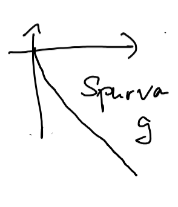
\includegraphics[width=0.2\linewidth]{figures/implizite_funktion_1_zu_2d_beispiel_spur}
          \label{fig:implizite_funktion_1_zu_2d_beispiel_spur}
        \end{figure}
      \end{beispiel*}
      \item \( f\maps \reals^n\times \reals\to \reals \), \( f(x,t)=t^n+\sum_{j=1}^{n}x_j t^{n-j} \), \( f(x,t)=0 \) \timplies \( t \) Nullstelle des Polynoms \( p_x(t)=f(x,t) \).

      Sei \( t_0 \) eine einfache Nullstelle. Dann ist \( D_2f(x,t_0)\neq 0 \), da \( p_x(t)=(t-t_0)q_x(t) \) und \( q_x(t_0)\neq 0 \) und somit \( D_2f(x,t_0)=q_x(t_0)+\cancel{(t_0-t_0)q_x'(t_0)} \).

      \timplies \texists  Umgebung \( U \) von \( x_0\in \reals^n \) und ein stetig differenzierbare Funktion \( g\maps U\to \reals \) mit \( f(x,g(x))=0 \) und \( g(x_0)=t_0 \) \timplies Die einfachen Nullstellen eines Polynoms hängen in stetig differenzierbarer Art von den Koeffizienten ab, \dh insbesondere hängen si stetig davon ab, \dh zu \( \varepsilon>0 \), \texists \( \delta>0 \) \sd \( \abs{t-t_0}=\abs{g(x)-g(x_0)}<\varepsilon \) für \( x\in \ball{\phi}{x_0}\subset U \). 
      \begin{beispiel*}
        \begin{description}
          \item[\( 3t^2-t \)] Einfache Nullstelle \( t_0=\frac{1}{3} \).
          \item[\( \frac{10}{3}t^2-t \)] Einfache Nullstelle \( t_0=\frac{3}{10} \). 
        \end{description}
      \end{beispiel*}
      \item Die Bedingung im Satz über implizite Funktionen ist \emph{nicht} notwendig. \( f(x,y)=y^2 \) erfüllt in \( (1,0) \) die Bedingung \( D_2 f(1,0) \) invertierbar \emph{nicht}, \( f(x,y)=0 \) besitzt aber die Auflösung \( g(x)=0\quad \forall 0 \).
  \end{enumerate}
\end{beispiele*}
\section{Der Satz von der Umkehrabbildung}
Sei \( f\maps U\to \reals^n \) stetig differenzierbar, \( U\subset \reals^n \). Gibt es einfach zu prüfende Kriterien, die garantieren, dass \( f \) umkehrbar ist mit stetig differenzierbarer Umkehrfunktion \( g\maps f(U)\to \reals^n \)?

Notwendiges Kriterium ist, dass \( \totalderivative{f}(x) \) invertierbar ist, da mit der Kettenregel aus \( g\circ f=\Id_u \) folgt \( \totalderivative{g}(f(x))\matrixmult \totalderivative{f}(x)=\mathds{1} \). Tatsächlich ist sogar folgendes hinreichend:

\begin{satz}\label{satz_von_der_umkehrabbildung}\index{Satz von der Umkehrabbildung}
  Sei \( U\subset \reals^n \) offen, \( f\maps U\to \reals^n \), stetig differenzierbar. Sei \( a\in U \) \sd \( \totalderivative{f}(a) \) invertierbar ist. Dann gibt es eine offene Umgebung \( V\subset U \) von \( a \) und eine offene Umgebung \( W\in \reals^n \) von \( b\definedas f(a) \), \sd \( f\maps V\to \reals^n \), \( V \) bijektiv auf \( W \) abbildet und die Umkehrabbildung \( g\maps W\to \reals^n \) stetig differenzierbar ist. Es gilt dann
  \begin{equation*}
    \totalderivative{g}(f(x))=\inverse{\totalderivative{f}(x)}\quad \forall x\in V.
  \end{equation*}
\end{satz}
\begin{bemerkung*}
  Die letzte Identität, die wir oben schon bewiesen hatten, leuchtet unmittelbar ein, wenn man sich überlegt, dass die Ableitung eine differenzierbare Funktion linear approximiert, und dass die Umkehrabbildung einer invertierbaren linearen Abbildung die inverse Matrix ist.
\end{bemerkung*}
\begin{proof}[Beweis von \ref{satz_von_der_umkehrabbildung}]
  Betrachte \( F\maps \reals^n\times U\to \reals^n \), \( F(z,x)=z-f(x) \). Dann ist 
  \begin{equation*}
    \totalderivative{F}(z,x) = (\underbrace{\mathds{1}_{n\times n}}_{D_1 F(z,x)}\, -\underbrace{\totalderivative{f}(x)}_{D_2 F(z,x)}).
  \end{equation*} 
  Wegen \( F(b,a)=0 \) und \( D_2 F(b,a)=-\totalderivative{f}(a) \) invertierbar können wir den Satz von der impliziten Funktion \ref{satz_von_der_impliziten_funktion} auf \( F \) anwenden und \( F \) nach \( x \) auflösen. Es gibt also offene Umgebungen \( V_1\subset \reals^n \) von \( b \) und \( V_2\subset U \) von \( a \) und eine stetig differenzierbare Funktion (\vgl Bemerkung~\ref{implizite_funktion_auf_umgebung_stetig_differenzierbar} nach    \ref{satz_von_der_impliziten_funktion}) \( g\maps V_1\to \reals^n \) mit \( g(V_1)\subset V_2 \) und \( F(z,g(z))=0\quad \forall z\in V_1 \), also \( z-f(g(z))=0 \quad \forall z\in V_1 \) und für all \( (z,x)\in V_1\times V_2 \) mit \( F(z,x)=0 \) gilt \( x=g(z) \).

  Setze nun
  \begin{gather*}
    V \begin{aligned}[t]
      &\definedas V_2\cap \explain{\text{Urbild von \( V_1 \)}}{\inverse{f}(V_1)}\\
      &=\Set{x\in V_2|f(x)\in V_1}.
    \end{aligned}
  \end{gather*}
  \( V \) ist offen (da \( f \) stetig und \( V_1,V_2 \) offen) und \( f \) bildet \( V \) bijektiv auf \( W\definedas V_1 \) ab und die Umkehrabbildung ist \( g \).
\end{proof}

Man sagt, wenn \( f \) wie oben ist: \enquote{\( f \) ist bei \( a \) \emph{lokal} umkehrbar.}
\begin{beispiele}
  \begin{enumerate}
    \item \( f(x)= \Ln{x} \), \( x>0 \), \( a=1 \), \( b=0 \), \( f'(1)=1 \).
    \begin{figure}[H]
      \centering
      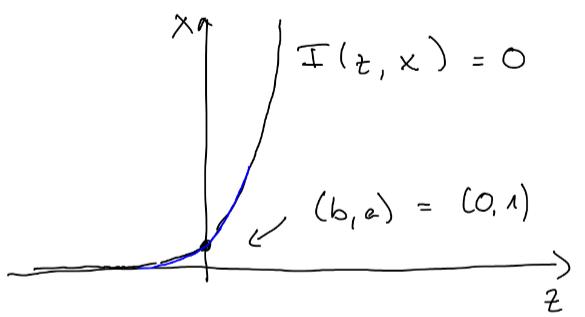
\includegraphics[width=0.5\linewidth]{figures/satz_von_der_umkehrungsfunktion_beispiel_ln}
      \caption*{\textcolor{Blue}{\( \Gamma_g=\Set{(z,g(z))|z\in V} \)}}
      \label{fig:satz_von_der_umkehrungsfunktion_beispiel_ln}
    \end{figure}
    \begin{gather*}
      g'(\Ln{x})=\inverse{\p*{ \frac{1}{x} }}=x\\
      g'(z)=g(z)\\
      \underset{(\text{\diffcourse{1}})}{\implies} g(z)=C\exp (z),
    \end{gather*}
    und wegen \( g(0)=1 \) folgt \( C=1 \).
    \item \( f(x)=3x^2-x \), \( f(1)=2 \), \( \totalderivative{f}(1)=5\neq 0 \).
    \begin{figure}[H]
      \centering
      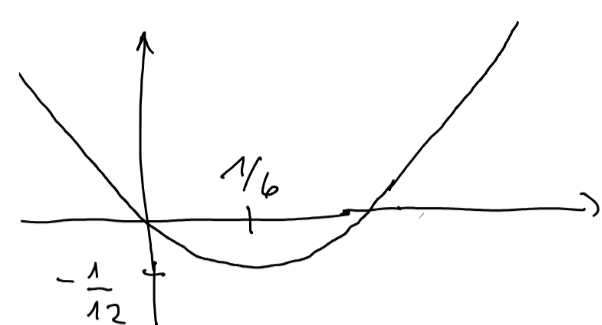
\includegraphics[width=0.5\linewidth]{figures/satz_von_der_umkehrungsfunktion_beispiel_parabel}
      \label{fig:satz_von_der_umkehrungsfunktion_beispiel_parabel}
    \end{figure}
    \begin{equation*}
      F(z,x)=z-f(x)\qquad N_f(0)=\Set{(f(x),x)|x\in U}
    \end{equation*}
    \begin{figure}[H]
      \centering
      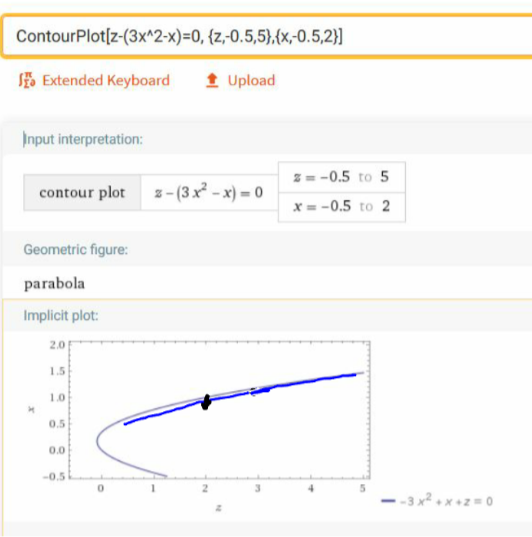
\includegraphics[width=0.5\linewidth]{figures/satz_von_der_umkehrungsfunktion_beispiel_parabel_umkehrung}
      \caption*{\( N_F(0) \), \textcolor{Blue}{\( \Gamma_g=\set{\underbrace{(z,g(z))}_{=(f(x),x)}|z\in W} \)}, von Wolfram Alpha.}
      \label{fig:satz_von_der_umkehrungsfunktion_beispiel_parabel_umkehrung}
    \end{figure}
    Die Rekursionsformel \( g_0(z)=a \), \( g_{j+1}(z)=a+h(z,g_j(z)) \),
    \begin{equation*}
      h(z,x)=x-\inverse{D_2 F(b,a)}\matrixmult F(z,x)
    \end{equation*}
    ist meist nicht sehr nützlich zur Bestimmung von \( g \). Aber die Ableitung von \( g \) können wir sofort bestimmen: \( \totalderivative{g}(z)=\inverse{\totalderivative{f}(g(z))} \) oder \( \totalderivative{g}(f(x))=\inverse{\totalderivative{f}(x)} \).

    Im Beispiel: \( g'(z)=\frac{1}{6g(z)-1} \) für \( g(z)\neq \quot{1}{6} \). \timplies Ansatz \( g(z)=\alpha+\sqrt{\beta+\gamma z} \)
    \begin{gather*}
      z\needed{=}f(g(z))=3(\alpha^2+\beta+\gamma z+2a\sqrt{\beta+\gamma z})-\alpha-\sqrt{\beta+\gamma z}\\
      \implies \begin{gathered}
        6\alpha = 1\\
        3\alpha^2+3\beta-\alpha=0\\
        3\gamma=1
    \end{gathered}\implies g(z)=\frac{1}{6}+\frac{1}{6}\sqrt{+1+12z}
    \end{gather*}
    auf \( \ointerval{-\frac{1}{12}}{\infty} \) definiert \timplies es muss \( f>-\frac{1}{12} \) sein, also ist das maximale \( V=\ointerval{\frac{1}{12}}{z} \).
    \item \( f\maps \reals_{>0}\times \reals\to \reals^2 \), \( (r,\phi)\mapsto \transpose-{(r\Cos{\phi}, r\Sin{\phi})} \).
    \begin{gather*}
      \Det \totalderivative{f}(r,\phi)=\begin{pNiceMatrix} \Cos{\phi} & -r\Sin{\phi}\\ \Sin{\phi}
       & r\Cos{\phi} \end{pNiceMatrix}\\
       \Det \totalderivative{f}(r,\phi)=r>0\quad \forall (r,\phi).
    \end{gather*}
    \timplies Bei allen \( r,\phi \) ist \( f \) lokal invertierbar. Es gilt
    \begin{equation*}
      \inverse{\totalderivative{f}(r,\phi)}=\begin{pNiceMatrix} \Cos{\phi} & \Sin{\phi}\\ -\frac{\Sin{\phi}}{r} & \frac{\Cos{\phi}}{r} \end{pNiceMatrix}.
    \end{equation*}
    Setze \( f(r,\phi)=\begin{pNiceMatrix} x \\ y \end{pNiceMatrix} \) \timplies \( r=\sqrt{x^2+y^2} \), \( \frac{x}{r}=\Cos{\phi} \), \( \frac{y}{r}=\Sin{\phi}\).
    \begin{equation*}
      \implies \inverse{\totalderivative{f}(r,\phi)}=\totalderivative{f}(\underbrace{f(r,\phi)}_{=\begin{pNiceMatrix} x \\ y \end{pNiceMatrix}})=\begin{pNiceMatrix} \frac{x}{\sqrt{x^2+y^2}} & \frac{y}{\sqrt{x^2+y^2}} \\ \frac{-y}{x^2+y^2} & \frac{x}{x^2+y^2} \end{pNiceMatrix}
    \end{equation*}
    mit \( g  \) eine lokale Umkehrung.

    \begin{beachte*}
      \( f(\reals_{>0}\times \reals)=\reals^2\setminus \zeroset \), aber es gibt \emph{keine } globale Umkehrfunktion \( g\maps \reals^2\setminus \zeroset \to \reals^2 \), denn \( f(r,\phi+k2\pi)=f(r,\phi) \quad \forall k\in \wholes \), also \( f \) nicht injektiv. Man kann maximal Intervalle der Länge \( 2\pi \) (in \( \phi \)) betrachten.

      Betrachte etwa \( U=\reals_{>0}\times \ointerval{-\pi}{\pi} \). Das wird unter \( f \) bijektiv auf \( W=\reals^2\setminus \Set{(x,0)|x\leq 0} \) abgebildet.
      \begin{figure}[H]
        \centering
        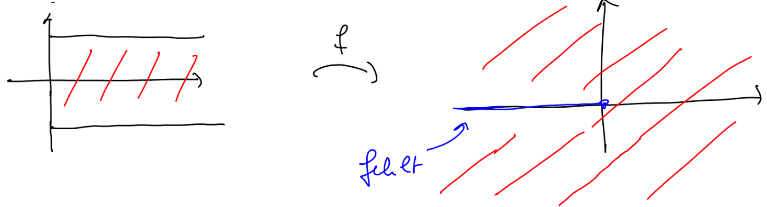
\includegraphics[width=0.5\linewidth]{figures/geschlitzte_ebene}
        \caption*{\enquote{geschlitzte Ebene}}
        \label{fig:geschlitzte_ebene}
      \end{figure}
      Wie kommt man darauf, dass \( f \) \( V \) auf \( W \) abbildet? \( \phi \) ist entweder \( \neq 0 \), dann ist \( r\Sin{\phi}\in \ointerval{-r}{0}\cup \ointerval{0}{r} \), oder \( \phi=0 \), dann ist \( r\Cos{\phi}=r>0 \).

      \minisec{\( \evaluateat{f}{U} \) ist injektiv:} Ist \( r\Cos{\phi}=r'\Cos{\phi}' \) und \( r\Sin{\phi}=r'\Sin{\phi}' \), so ist \( r^2=r'^2 \) \timplies (da, \( r,r'>0 \)) \( r=r' \) und aus \( \Cos{\phi}=\Cos{\phi}' \) folgt zunächst \( \phi=\pm \phi' \), aber aus \( \Sin{\phi}=\Sin{\phi}'=\pm \Sin{\phi}\)folgt \( \phi=+\phi' \).

      \minisec{\( \evaluateat{f}{U} \) bildet surjektiv auf \( W \) ab:} Sei \( \begin{pNiceMatrix} x \\ y \end{pNiceMatrix} \in W \), \dh es ist \( y\neq 0 \) oder \( x>0 \) \timplies \( r=\set{x^2+y^2}>0 \) \timplies \( \p*{ \frac{x}{r} }^2+\p*{ \frac{y}{r} }^2=1 \) \timplies \( \abs{\quot{x}{r}}\leq 1 \). Es ist \( \quot{x}{r}\neq -1 \), denn sonst wäre \( \quot{y}{r}=0 \), aber \( (-1,0)\notin W \). Somit ist \( y=0 \) \tiff \( \quot{x}{r}=1 \) und wir legen einen Winkel \( \phi \) fest mit \( \Cos{\phi}=\quot{x}{r} \). \( \phi\in \ointerval{-\pi
        }{0} \), falls \( y<0 \), oder \( \ointerval{0}{\pi} \), alls \( y>0 \), oder \( \phi=0 \), falls \( y=0. \)

      \begin{behauptung*}
        Für diesen Winkel gilt \( \Sin{\phi}=\quot{y}{r} \).
      \end{behauptung*}
      \begin{proof}
        \begin{equation*}
          \Sin{\phi}=\sgn{\Sin{\phi}}\sqrt{\sin^2 \phi}=\sgn{y}\sqrt{1-\cos^2 \phi}=\sgn{y}\sqrt{1-\quot{x^2}{r^2}}=\sgn{y}\quot{\abs{y}}{r}=\quot{y}{r}.
        \end{equation*}
      \end{proof}
      Ist man nicht an einer maximalen Umgebung von \( \ointerval{r_0}{\phi_0}  \) interessiert, kann man so schneller zum Ziel:

      Ist beispielsweise \( -\quot{\pi}{2}<\phi_0<\quot{\pi}{2} \) betrachte \( \phi\in \ointerval{-\quot{\pi}{2}}{\quot{\pi}{2}} \),woraus \( x>0 \) folgt, so dass man recht schnell rät, dass \( f \) \( V\definedas \reals_{>0}\times  \ointerval{-\quot{\pi}{2}}{\quot{\pi}{2}} \) bijektiv auf \( W=\reals_{>0}\times \reals \) abbildet, indem man sich überlegt, dass die Umkehrfunktion \( g \) durch \( g(x,y)=\transpose-{(\sqrt{x^2+y^2}, \ArcTan{\quot{y}{x})}} \) gegeben ist (wohldefiniert für \( x>0 \)), da 
      \begin{equation*}
        g(r \Cos{\phi}, r\Sin{\phi})=(r,\underbrace{\ArcTan{\quot{\Sin{\phi}}{\Cos{\phi}}_{=\phi}}})
      \end{equation*}
      und es ist klar, dass \( g \) \( W \) bijektiv au \( V \) abbildet, da \( \ArcTan;\maps \reals\to \ointerval{-\quot{\pi}{2}}{\quot{\pi}{2}} \) bijektiv ist, \sd  wenn \( \ArcTan{\quot{x}{y}}=\ArcTan{\quot{\tilde{x}}{\tilde{y}}} \) gilt \( y=\quot{\tilde{yx}}{x} \) und dann
      \begin{equation*}
        \sqrt{x^2+y^2}=\sqrt{x^2+\frac{\tilde{y}^2 x^2}{\tilde{x}^2}}=\frac{x}{\tilde{x}}\sqrt{\tilde{x}^2+\tilde{y}^2}
      \end{equation*}
      nut gleich \( \sqrt{\tilde{x}^2+\tilde{y}^2} \), wenn \( x=\tilde{x} \) (und somit \( y= \tilde{y}\)) und \( \reals_{>0}\times\reals\ni (x,y)\mapsto \sqrt{x^2+y^2} \) bildet surjektiv auf \( \reals_{>0} \) ab (da streng monoton wachsend).
    \end{beachte*}
  \end{enumerate}
\end{beispiele}
Es folgen einige etwas tiefsinnigere Folgen aus dem Umkehrsatz.
\begin{satz}\label{offene_abbildungen_satz}
  Sei \( f\maps U\to \reals^n \) stetig differenzierbar, \( U\subset \reals^n \) offen. Sei \( V\subset U \) offen. Ist \( \totalderivative{f}(x) \) invertierbar für alle \( x\in V \), so ist \( \evaluateat{f}{V} \) eine \emph{offene Abbildung}, \dh offene Teilmengen \tsubset \( V \) auf offene Mengen abgebildet.
\end{satz}
\begin{antibeispiel*}
  \( f\maps \ointerval{0}{1}\to \reals \), \( f(x)=1\quad \forall x \). \( f'(x)=0 \) nicht invertierbar. \( \Set{1} \) nicht offen in \( \reals \).
\end{antibeispiel*}
\begin{proof}[Beweis von \ref{offene_abbildungen_satz}]
  Sei \( \tilde{V}\subset U \) offen, dann ist \( \tilde{V}  \) auch offen \( U \). Sei \( b\in f(\tilde{V}) \). Wähle ein \( a\in \tilde{V} \) \sd \( b=f(a) \). Wende den Satz von der lokalen Umkehrfunktion auf \( \evaluateat{f}{\tilde{V}} \) an \timplies \texists  offene Umgebungen \( V_1\subset \tilde{V} \) und \( W\subset \reals^n \) von \( a \) beziehungsweise \( b \) \sd \( \evaluateat{f}{V_1} \) umkehrbar ist mit \( g\maps W\to \reals^n \) und insbesondere \( f \) \( V_1 \) bijektiv auf \( W \) abbildet. Somit gilt \( W=f(V_1)\subset f(\tilde{V}) \) und ist Umgebung von \( b \) \timplies \( f(\tilde{V}) \) ist offen.
\end{proof}
\begin{satz}[Minimum- / Maximum-Prinzip]\label{extremumprinzip}\index{Minimum- / Maximum-Prinzip}
  Sei \( f\maps U\to \reals^n \), \( U\subset \reals^n \), stetig differenzierbar. Sei \( V\subset U \) offen und sei \( \totalderivative{f}(x) \) invertierbar für alle \( x\in V \). Dann gilt für die Funktion
  \begin{equation*}
    V\ni x\mapsto \norm{f(x)}
  \end{equation*}
  \begin{enumerate}
    \item \label{extremumprinzip:kein_maximum} Sie besitzt kein Maximum.
    \item \label{extremumprinzip:kein_minimum_wenn_nicht_null} Ist \( f(x)\neq 0\quad \forall x\in V \) besitzt sie kein Minimum.
  \end{enumerate}
\end{satz}
\begin{beachte*}
  Man kann den Beweis dieses Satzes auf \ref{extremum_notwendige_bedingung} zurückführen, obwohl \( \norm{\cdot} \) nur auf \( \reals^n\setminus \zeroset  \) partiell differenzierbar ist. Wir wollen hier dennoch anders vorgehen:
\end{beachte*}
\begin{proof}
  \begin{proofdescription}
    \item[\ref{extremumprinzip:kein_maximum}] Angenommen \( a \) ist Maximalstelle von \( \norm{f} \). Dann ist \( f(a)\neq 0 \), da sonst \( \norm{f(x)}=0\quad \forall x\in V \) und somit \( \evaluateat{f}{V}=0 \) und \( \totalderivative{f}(x)=0\quad \forall x\in V \). \ref{offene_abbildungen_satz} \timplies \texists  \( \varepsilon>0 \) \sd \( \ball;{\varepsilon}(f(a))\subset f(V) \). Setze \( b\definedas f(a)+\rho f(a) \) mit\( \rho=\quot{\varepsilon}{2\norm{f(a)}} \) 
    \begin{align*}
      \implies &\norm{b-f(a)}=\rho\norm{f(a)}=\quot{\varepsilon}{2}<\varepsilon\\
      \implies &b\in \ball;{\varepsilon}\implies \exists x_0\in V  \logicspace \text{\sd}\logicspace b=f(x_0)\\
      \implies &\norm{f(x_0)}=\norm{b}=(1+\rho)\norm{f(a)}>\norm{f(a)}.
    \end{align*}
    \item[\ref{extremumprinzip:kein_minimum_wenn_nicht_null}] Analog mit \( b=f(a)-\rho f(a) \).
  \end{proofdescription}
  
\end{proof}

% !TEX root = ./Vorlesungsmitschrift DIFF 2.tex  
\lecture{Do 21.05. 10:15}{}
\section{Lokale Extrema unter Nebenbedingungen}
Wir betrachten folgende Situation:\\
Wir suchen Extremstellen einer Funktion \( f \) unter gewissen Nebenbedingungen \zb 
\begin{enumerate}[label=\rechtsklammer{\alph*}]
  \item\label{nebenbedingung_extremum:beispiel:mikro} (Mikro-Ökonomie) Es soll das Maximum einer Nutzenfunktion \( f(x,y)=\sqrt{xy} \), \( x>0 \), \( y>0 \), unter der Budgetbedingung \( 64=2x+8y \) bestimmt werden.
  \item\label{nebenbedingung_extremum:beispiel:geometrie} (Geometrie) Welches Dreieck kopfüber im Halbkreis hat den größten Flächeinhalt? Also \( f(b,h)=\frac{1}{2}bh \) unter dr Nebenbedingung \( \frac{1}{4}b^2+h^2=r^2 \) (Pythagoras).
  \begin{figure}[H]
    \centering
    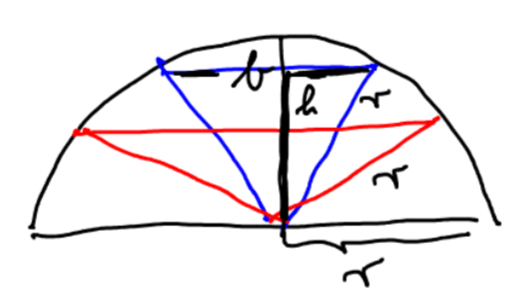
\includegraphics[width=0.4\linewidth]{figures/dreiecksmaximierung}
    \label{fig:dreiecksmaximierung}
  \end{figure}
  \item Berücksichtige, dass eine Bewegung eingeschränkt ist, \zb auf dem Innenrand einer Kugelschale (Nebenbedingung: \( x^2+y^2+z^2=r^2 \)).
\end{enumerate}
Mathematisch geht es um folgendes Problem:
\begin{definition}\label{nebenbedingung_extremum}\index{Lokales Extremum unter Nebenbedingung}
  Sei \( U\subset \reals^n \) offen, \( f\maps U\to \reals \), sei \( h\maps U\to \reals^m \). Dann sagen wir \( f \) hat in \( a\in U \) ein \emph{lokales Maximum \bzw Minimum} (Extremum) \emph{unter der Nebenbedingung} \( h(x)=0 \), wenn: \( a\in N_h(0) \) und es eine Umgebung \( U_0 \) von \( a \) gibt \sd \( f(a)\geq f(x) \) \bzw \( f(a)\leq f(x) \) \tforall \( x\in U_0 \cap N_h(0) \).
\end{definition}
In einfachen Fällen kann man die Nebenbedingung direkt auflösen und die (\ref{satz_von_der_impliziten_funktion:hoehenlinie_folgerung}) Funktion einsetzen, \zb in \ref{nebenbedingung_extremum:beispiel:mikro}
\begin{equation*}
  y=8-\frac{1}{4}x\qquad f(x,8-\quot{1}{4}x)=\sqrt{x(8-\quot{x}{4})}.
\end{equation*}
Allgemeiner: Sei \( f \), \( h \) wie in \ref{nebenbedingung_extremum} und zudem \( f \) differenzierbar und \( h\maps U\to \reals^m \), \( U\subset \reals^{n-m}\times \reals^m \), erfülle in \( a=(a_1,a_2)\in N_h(0) \) die Bedingungen des Satzes über implizite Funktionen. Also gibt es Umgebungen \( V_1 \) von \( a_1 \) und \( V_2 \) von \( a_2 \) und eine stetig differenzierbare Funktion \( g\maps V_1\to V_2 \) \sd \( N_h(0)\cap V_1\times V_2=\Set{(u,g(u))|u\in V_1} \). Also besitzt in diesem Fall \( f \) eine lokales Extremum in \( a \) unter der Nebenbedingung \( h=0 \) genau dann, wenn \( u\mapsto f(u,g(u)) \) ein lokales Extremum in \( a_1 \) besitzt.

Dies führt zur sogenannten 
\begin{satz}[Lagrange-Multiplikator-Regel]
  Sei \( f\maps U\to \reals \), \( U\subset \reals^n \) offen, in \( a\in U \) differenzierbar. Sei \( h\maps U\to \reals^m \) stetig differenzierbar, \( m<n \). Es sei \( \rang-{\totalderivative{h}(a)}=m \).

  Es besitze \( f \) in \( a \) unter der Nebenbedingung \( h(x)=0 \) ein lokales Extremum. Dann gibt es \( \lambda_1,\dotsc,\lambda_m\in \reals \) (\emph{Lagrange-Multiplikatoren}), \sd 
  \begin{equation*}
    \grad{f(a)}=\lambda_1 \grad{h_1(a)}+\dotsb+\lambda_m \grad{h_m(a)}.
  \end{equation*}
\end{satz}
\begin{proof}
  Sei \obda \( U=U_1\times U_2 \) mit \( U_1\subset \reals^{n-m} \), \( U_2\subset \reals^m \), \( a=(a_1,a_2)\in U_1\times U_2 \), (Notation \( (x,y)\in U_1\times U_2 \)) und \( \totalderivative{h}(x,y)=(D_1h(x,y) \quad  \braceannotate{\mathclap{\in \sqmatrices{m}{\reals}}}{D_2 h(x,y)})\vphantom{\underbrace{D_2 h(x,y)}_{\in \sqmatrices{m}{\reals}}} \) mit \( D_2h(a_1,a_2) \) invertierbar.
    
  \thref{satz_von_der_impliziten_funktion} \timplies \texists  \( V_1 \) offene Umgebung von \( a_1 \), \( V_2 \) offene Umgebung von \( a_2 \), \( g\maps V_1\to \reals^m \) stetig differenzierbar, \( g(V_1)\subset V_2 \), \( \totalderivative{g}(x)=-\inverse{D_2 h(x,g(x)) }\matrixmult D_1 h(x,g(x))\) und 
  \begin{equation*}
    N_h(0)\cap V_1\times V_2=\Set{(x,g(x))|x\in V_1}.
  \end{equation*}
  \( a \) ist lokale Extremstelle von \( f  \) unter der Nebenbedingung \( h(x)=0 \) \timplies \( a_1 \) ist lokale Extremstelle von
  \begin{equation*}
    V_1\ni u\mapsto f(u,g(u))=f\circ \begin{pNiceMatrix} \Id \\ g \end{pNiceMatrix}(u)
  \end{equation*}
  \timplies (Kettenregel und \ref{extremum_notwendige_bedingung})
  \begin{align*}
    &0\begin{aligned}[t]
      &=D{f\circ \begin{pNiceMatrix} \Id \\ g \end{pNiceMatrix}}(a_1)\\
      &=\totalderivative{f}(a_1,g(a_1))\matrixmult \begin{pNiceMatrix} \mathds{1}_{n-m} \\ \totalderivative{g} \end{pNiceMatrix}(a_1)\\
      &=D_1 f(a_1,a_2)-\braceannotate{(1\times m)\text{ mal }(m\times m)=(1\times m)\defines (\lambda_1,\dotsc,\lambda_m)}{D_2  f(a_1,a_2)\matrixmult \inverse{D_2 h(a_1,a_2)}}\matrixmult D_1 h(a_1,a_2)\vphantom{\underbrace{M}_{M}}
    \end{aligned}\\
    \implies &D_1 f(a)\begin{aligned}[t]
      &=(\lambda_1,\dotsc,\lambda_m )\matrixmult D_1 h(a)\\
      &=(\lambda_1,\dotsc,\lambda_m)\matrixmult \begin{pNiceMatrix} \partial_1 h_1 &  \Cdots  & \partial_{n-m}h_1 \\ \Vdots &  & \Vdots \\ \partial_1 h_m & \Cdots & \partial_{n-m} h_m \end{pNiceMatrix}(a)\\
      &=\p*{ \sum_{j=1}^{m}\lambda_j \partial_1 h_j, \sum_{j=1}^{m}\lambda_j \partial_2 h_j,\dotsc,\sum_{j=1}^{mm}\lambda_j \partial_{n-m}h_j }\\
      &=\sum_{j=1}^{m}\lambda_j D_1 h_j(a).
    \end{aligned}
  \end{align*}
  Gleichzeitig gilt (Definition der \( \lambda_j \))
  \begin{equation}
    D_2 f(a_1,a_2)\matrixmult\inverse{D_j h(a_1,a_2)}\defines (\lambda_1,\dotsc,\lambda_m),
  \end{equation}
  also (wie oben)
  \begin{align*}
    &D_2 f(a_1,a_2)=(\lambda_1,\dotsc,\lambda_m)\matrixmult D_2h(a)=\sum_{j=1}^{m}\lambda_j D_2 h_j(a)\\
    \implies &\begin{pNiceMatrix} D_1 f(a) & D_2 f(a) \end{pNiceMatrix}= \sum_{j=1}^{m} \lambda_j \begin{pNiceMatrix} D_1 h_j(a) & D_2 h_j(a) \end{pNiceMatrix}.
  \end{align*}
\end{proof}
Wir nutzt man diesen Satz zur Lösung von Problemen wie oben?
\begin{bemerkung}
  Unter Voraussetzungen an \( f \) und \( h \) wie oben betrachte das Gleichungssystem 
  \begin{gather}
    \tag{\( * \)}\label{eq:lagrange_multiplikatoren_gleichungssystem}\left.\begin{aligned}
      \partial_{\textcolor{blue}{1}}f(a)+\lambda_1\partial_{\textcolor{blue}{1}} h_1(a)+\dotsb+\lambda_m \partial_{\textcolor{blue}{1}} h_m(a)&=0\\
      \partial_{\textcolor{blue}{2}}f(a)+\lambda_1\partial_{\textcolor{blue}{2}} h_1(a)+\dotsb+\lambda_m \partial_{\textcolor{blue}{2}} h_m(a)&=0\\
      &\vdots\\
      \partial_{\textcolor{blue}{n}}f(a)+\lambda_1\partial_{\textcolor{blue}{n}} h_1(a)+\dotsb+\lambda_m \partial_{\textcolor{blue}{n}} h_m(a)&=0\\
      h_1(a)&=0\\
      &\vdots\\
      h_m(a)&=0
    \end{aligned}\right\}
  \end{gather}
  \eqref{eq:lagrange_multiplikatoren_gleichungssystem} ist gleichbedeutend mit
  \begin{equation*}
    \tag{\( ** \)} \label{eq:lagrange_multiplikatoren_kompakt}\totalderivative{f}(a)=0,
  \end{equation*}
  wenn \( F(a,\lambda)=f(a)+\sum_{j=1}^{m}\lambda_j h_j(a) \), denn \( D_1 F=0 \) liefert die ersten \( n \) Zeilen von \eqref{eq:lagrange_multiplikatoren_gleichungssystem}, \( D_2 F=0 \) lieft die letzten \( m \) Zeilen von \eqref{eq:lagrange_multiplikatoren_gleichungssystem}.

  Man versucht dann \eqref{eq:lagrange_multiplikatoren_gleichungssystem} oder \eqref{eq:lagrange_multiplikatoren_kompakt} zu lösen.
\end{bemerkung}
\begin{beispiele*}
  \begin{enumerate}
    \item Zunächst \ref{nebenbedingung_extremum:beispiel:geometrie} von oben. \( f\maps \reals_{>0}\times \reals_{>0}\to \reals \), \( f(b,h)=\frac{1}{2}bh \), \( H(b,h)=\frac{1}{4}b^2+h^2-r^2 \). \( a=(b,h) \). \( \totalderivative{f}(a)=\p*{ \frac{1}{2}h,\frac{1}{2}b } \), \( DH(a)=\p*{ \frac{1}{2}b, 2h } \). \( h>0 \) \timplies die Voraussetzungen des Satzes sind erfüllt.
    \begin{align*}
      \tag{\(*\)}&\left.\begin{aligned}
        \partial_1 f(a)+\lambda \partial_1 H(a)=\frac{1}{2}h+\frac{1}{2}b&\needed{=}0\\
        \partial_2 f(a)+\lambda\partial_2 H(a)=\frac{1}{2}b+\lambda 2H&\needed{=}0\\
        H(a)=\frac{1}{4}b^2+h^2-r^2&=0
      \end{aligned}\right\}\\
      \implies &\lambda=-\quot{b}{4h}\quad h=\quot{b^2}{4h} \implies 4h^2=b^2\\
      \underset{\text{3.\ Zeile}}{\implies} &\frac{1}{2}b^2=r^2\implies b=\sqrt{2}\quad h=\frac{1}{\sqrt{2}r}.
    \end{align*}
    \begin{figure}[H]
      \centering
      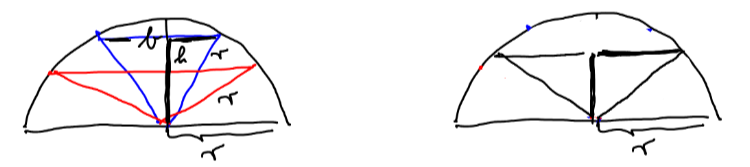
\includegraphics[width=0.5\linewidth]{figures/dreiecksmaximierung_antwort}
      \label{fig:dreiecksmaximierung_antwort}
    \end{figure}
    Der Flächeninhalt wird maximal \( \quot{1}{2}r^2 \), denn für \( b\goesto 0 \) (spitzerwerdendes Dreieck), strebt \( f\goesto 0 \), ebenso für \( h\goesto 0 \) (breiterwerdendes Dreieck).
    \item Sei \( A\in \sqmatrices{n}{\reals} \) symmetrisch. Sei \( f(x)\definedas \scalarproduct{x}{Ax} \) die zugehörige quadratische Form. Gesucht: Extrema von \( f \) unter der Nebenbedingung \( h(x)=\norm{x}_E^2-1=0 \). \( \totalderivative{h}(x)=2x\neq 0 \) \tforall \( x \) in \( N_h(0) \). Wir können also unseren Satz anwenden
    \begin{align*}
      \totalderivative{f}(a)=2A\matrixmult a\\
      \tag{\(*\)} 2A\matrixmult a+\lambda 2a\needed{=}0
    \end{align*}
    und \( \norm{a}_E=1 \). Das heißt notwendig für das Vorliegen einer Extremstelle ist, dass \( a \) Eigenvektor ist. Da \( A \) symmetrisch, ist \( A \) diagonalisierbar \timplies \texists  Eigenvektoren \( v_1,\dotsc, v_n \). Wegen \( f(v_j)=\scalarproduct{v_j}{A v_j}=\lambda_j \) Eigenwert folgt: \( f \) wird maximiert von normierten Eigenvektoren zum größten Eigenwert und minimiert von denen zum kleinsten Eigenwert.
    \item Gesucht ist der Punkt in der Ebene
    \begin{equation*}
      E=\Set{\transpose-{(x_1,x_2,x_3)}\in \reals^3|x_1+x_2-x_3=0},
    \end{equation*}
    der von Punkt \( \transpose-{(1,0,0)} \) den kleinsten Abstand hat. Da \( \Set{\transpose-{(1,0,0)}} \) kompakt ist und \( E \) abgeschlossen, gibt es einen solchen (\vgl unser Beispiel nach \thref{funktion_von_kompaktem_metrischen_raum_zu_r_kriegt_min_max}). Wir wollen also \( f(x)=\norm{x-e_1}_E^2 \) minimieren unter der Neben-Bedingung \( h(x)=x_1+x_2-x_2=0 \).

    \( \totalderivative{h}(a)=\begin{pNiceMatrix} 1 & 1 & -1 \end{pNiceMatrix} \) hat maximalen Rang (\( 1 \)) \dh jeder gesuchte Punkt \( a  \) muss erfüllen
      \begin{align*}
        2(a_1-1)+\lambda&=0\\
        2a_2+\lambda&=0\\
        2a_3-\lambda&=0\\
        a_1+a_2-a_3&=0,
      \end{align*}
    also ist \( a=\begin{pNiceMatrix} \quot{2}{3} & -\quot{1}{3} & \quot{1}{3} \end{pNiceMatrix} \) der einzige Kandidat für ein Extremum. Da es ein Minimum gibt, muss \( a \) dieses sein.
    \end{enumerate}
\end{beispiele*}
\section{Höhere Ableitungen, Taylorformel}
Ist \( f\maps U\to \reals^m \), \( U\subset \reals^n \) offen, stetig differenzierbar, kann man sich fragen, obe auch die Ableitung \( U\ni x\mapsto \totalderivative{f}(x) \) als Funktion \( \totalderivative{f}\maps U\to \matrices{m}{n}{\reals} \) wieder differenzierbar ist (in \( a \), auf ganz \( U \), auf \( V\subset U \) \dots), also ob es eine \emph{lineare} Abbildung \( A\maps \reals^n\to \matrices{m}{n}{\reals} \) gibt, \sd 
\begin{equation*}
  \totalderivative{f}(a+h)=\totalderivative{f}(a)+A(h)*\underline{R}_a^{\totalderivative{f}}(h)
\end{equation*}
mit \( \frac{\underline{R}_a^{\totalderivative{f}}(h)}{\norm{h}}\goesto 0 \) wenn \( h\goesto 0 \). Hier ist \( \underline{R}_a^{\totalderivative{f}}\maps B_{\delta}(0)\to \matrices{m}{n}{\reals} \). 

Benennt man \( \totalderivative{f}\defines g \) sieht man schnell, dass alle Sätze über differenzierbare Abbildungen natürlich auf für \( g \) gelten, insbesondere die Eindeutigkeit der Abbildung, wenn sie existiert, Kettenregel \etc. Nur kann man, wenn man nicht den Raum \( \matrices{m}{n}{\reals} \) mit \( \reals^{m\cdot n} \), die Ausdrücke im Allgemeinen nicht mehr so leicht hinschreiben, etwa \( A(h) \) als Produkt einer Matrix mit dem Vektor \( h \).

Ist \( m=1 \) oder betrachtet man nur die Komponentenfunktionen einer \( \reals^m \)-wertigen Funktion, sieht man jedoch:
\begin{equation*}
  g\definedas \totalderivative{f}\maps U\to \matrices{1}{n}{\reals}
\end{equation*}
nimmt Werte in den \( 1\times n \)-Matrizen an, identifiziert man nun \( \matrices{1}{n}{\reals}\simeq \reals^n \) (Spaltenvektor), hat man es mit einer Funktion \( g\maps U \to \reals^n \) zu tun.

Einen \emph{Kandidaten} für \( \totalderivative{g}(a) \) findet man wieder über die partiellen Ableitungen
\begin{equation}
  \begin{pNiceMatrix} \partial_1 g(a) & \Cdots & \partial_n g(a) \end{pNiceMatrix}\in \sqmatrices{n}{\reals}
\end{equation}
und
\begin{equation*}
  g(x)=\begin{pNiceMatrix} \partial_1 f(x) \\ \Vdots \\ \partial_n f(x) \end{pNiceMatrix}
\end{equation*}
(wenn sie existieren). Insgesamt also
\begin{equation*}
  \begin{pNiceMatrix}
    \partial_1^2 f(a) & \partial_2 \partial_1 (a) & \Cdots & \partial_n \partial_1 f(a) \\
    \partial_1\partial_2 f(a) & \partial_2^2 (a) & \Cdots & \partial_n \partial_2 f(a) \\
    \Vdots & & & \Vdots\\
    \partial_1 \partial_n f(a) & \partial_2 \partial_n f(a) & \Cdots & \partial_n^2 f(a)
  \end{pNiceMatrix}\defines A
\end{equation*}
mit der Notation \( \partial_j \partial_i f(a)=\partial_j g_i(a)=\partial_j(\partial_i f)(a) \) und \( \partial_j^2=\partial_j \partial_j \).

Dann berechnet man den Rest wie üblich:
\begin{equation*}
  g(a+h)=g(a)+A\matrixmult h+ \underline{R}_a^g(h)
\end{equation*}
und überprüft, ob \( \frac{\underline{R}_a^g(h)}{\norm{h}}\goesto 0 \) für \( h\goesto 0 \).

Oder man überprüft, ob die partiellen Ableitungen stetig sind. Wenn ja, folgt die Differenzierbarkeit von \( \totalderivative{f} \) aus \thref{stetige_partielle_zu_ableitung}.

Wenn nein, muss man prüfen, ob \( \underline{R}_a^g \) das richtige Verhalten bei \( 0 \) hat. Wir werden allerdings bei den sogenannten höheren Ableitungen (wie der 2.\ Ableitung oben) meist stetig differenzierbare Funktionen betrachten.

\begin{definition}\index{$k$-fache partielle Differenzierbarkeit}
  \( f\maps U\to \reals \), \( U\subset \reals^n \) offen, heißt in \( a \) \emph{\( k \)-fach partiell differenzierbar}, wenn alle partiellen Ableitungen
  \begin{equation*}
    \partial_{j_1} f(a), \partial_{j_1} \partial_{j_2} f(a),\dotsc, \partial_{j_1}\partial_{j_2}\dotsb\partial_{j_k} f(a)
  \end{equation*}
  (Notation wie oben) \( j_i\in \Set{1,\dotsc,n} \) existieren.
  \begin{achtung*}
    Beachte, dass man zur Berechnung einer partiellen Ableitung die Funktion in einer Umgebung des Punktes kennen muss. Um also etwa eine \( k \)-te partielle Ableitung von \( f \) in \( a \) zu berechnen, muss man die \( (k-1) \)-te partielle Ableitung in einer Umgebung von \( a \) kennen.
  \end{achtung*}
  Ist \( f \) auf \( U \) \( k \)-fach partiell differenzierbar und sind alle partiellen Ableitungen der Ordnung \( \leq k \) stetig, so heißt \( f \) \emph{\( k \)-fach stetig partiell differenzierbar}.
\end{definition}
\begin{beispiel*}
  \( f(x_1,\dotsc,x_4)=x_1^3+x_2^2x_3-3x_4x_2 \). \( \partial_1^2 f(x)=6x_1 \), \( \partial_2^2 \partial_4 f(x)=\partial_2^2(-3x_2)=0 \),
  \begin{equation*}
    \partial_2 \partial_4 \partial_3 f(x)=\partial_2 \partial_4 (2x_2 x_3-3x_4)=\partial_2 (-3x_4)=0.
  \end{equation*}
  Dass die beiden letzt genannten Ableitungen gleich sind, ist kein Zufall:
\end{beispiel*}
\begin{satz}[Satz von Schwarz]\label{schwarzscher_satz}\index{Satz von Schwarz}
  Sei \( f\maps U\to \reals \), \( U\subset \reals^n \), zweimal stetig partiell differenzierbar. Dann gilt für alle \( a\in U \) und alle \( i,j\in \Set{1,\dotsc,n} \)
  \begin{equation*}
    \partial_j \partial_i f(a)=\partial_i \partial_j f(a).
  \end{equation*}
\end{satz}
\begin{proof}
  Sei \obda \( n=2 \), \( a=(a_1,a_2) \). \texists \( \delta>0 \) \sd \( B_{\delta}(a_1)\times \explain{\text{Intervall!}}{B_{\delta}(a_2)}\subset U \). Setze zu \( y\in B_\delta(a_2) \)
  \begin{equation*}
    F_y\maps B_\delta(a_1)\to \reals\qquad F_y(x)=f(x,y)-f(x,a_2).
  \end{equation*}
  MWS \timplies \texists  \( \zeta\in B_\delta(a_1)=\ointerval{a_1-\delta}{a_1+\delta} \) und zwar zwischen \( a_1 \) und \( x \) \sd 
  \begin{equation*}
    F_y(x)-F_y(a_1)=F_y'(\zeta)(x-a_1).
  \end{equation*}
  Es ist \( F_y'(\zeta)=\partial_1 f(\zeta,y)-\partial_1 f(\zeta,a_2) \). Betrachte die Funktion \( B_\delta(a_2)\ni y\mapsto \partial_1 f(\zeta,y) \). MWS \timplies \texists \( \eta\in B_\delta(a_2)=\ointerval{a_2-\delta}{a_2+\delta} \) und zwar zwischen \( a_2 \) und \( y \) \sd
  \begin{equation*}
    \partial_1 f(\zeta,y)-\partial_1 f(\zeta,a_2)=\partial_2 (\partial_1 f)(\zeta,\eta)(y-a_2).
  \end{equation*}
  Insgesamt folgt:
  \begin{equation*}
    f(x,y)-f(x,a_2)-f(a_1,y)+f(a)=\partial_2\partial_1 f(\zeta,\eta)(y-a_2)\matrixmult(x-a_1)\tag{\(*\)}.\label{eq:schwarzscher_satz:beweis:mws_1}
  \end{equation*}
  Dieselbe Konstruktion nehmen wir nun zu festen \( x\in B_\delta(a_1) \) für \( G_x(y)=f(x,y)-f(a_1,y) \) vor.

  \minisec{MWS:}
  \texists \( \tilde{\eta}\in \ointerval{a_2-\delta}{a_2+\delta} \) zwischen \( a_2 \) und \( y \) \sd \( G_x(y)-G_x(a_2)=G'x(\eta)(y-a_2) \). Es ist \( G_x'(\tilde{\eta})=\partial_2 f(x,\tilde{\eta})-\partial_2 f(a_1,\tilde{\eta}) \).

  \minisec{MWS:} 
  \texists \( \tilde{\zeta}\in \ointerval{a_1-\delta}{a_1+\delta} \) zwischen \( a_1  \) und \( x \) \sd\( \partial_2 f(x,\tilde{\eta})-\partial_2(a_1,\tilde{\eta})=\partial_1(\partial_2 f)(\tilde{\zeta},\tilde{\eta})(x-a_1) \).
  \begin{equation}
    f(x,y)-f(a_1,y)-f(x,a_2)+f(a)=\partial_1 \partial_2 f(\tilde{\zeta},\tilde{\eta})(y-a_2)\matrixmult(x-a_1)\tag{\(**\)}.\label{eq:schwarzscher_satz:beweis:mws_2}
  \end{equation}
  Aus \eqref{eq:schwarzscher_satz:beweis:mws_1} und \eqref{eq:schwarzscher_satz:beweis:mws_2} folgt für \( x\neq a_1 \), \( y\neq a_2 \)
  \begin{equation*}
    \partial_2 \partial_1 f(\tilde{\zeta},\tilde{\eta})=\partial_1 \partial_2 f(\zeta,\eta),
  \end{equation*}
  mit \( \zeta,\tilde{\zeta} \) zwischen \( a_1 \) und \( x \) und \( \eta,\tilde{\eta} \) zwischen \( a_2  \) und \( y \).

  Grenzübergang \( x\goesto a_1 \) und \( y\goesto a_2 \) liefert wegen der Stetigkeit von \( \partial_2\partial_1 f \) und \( \partial_1 \partial_2  \) die \Beh.
\end{proof}
\begin{antibeispiel*}
  \begin{equation*}
    f(x,y)=\begin{cases}
      xy\frac{x^2-y^2}{x^2+y^2}&(x,y)\neq (0,0)\\
      0 &(x,y)=(0,0)
    \end{cases}
  \end{equation*}
  Es gilt \( \partial_2 \partial_1 f(0,0)\neq \partial_1 \partial_2 f(0,0) \). Denn partielle Ableitung in \( 0 \):
  \begin{equation*}
    \partial_1 f(0,0)=\lim_{h \goesto 0}\frac{f(h,0)-f(0,0)}{h}=0=\partial_2 f(0,0).
  \end{equation*}
  Um die zweiten Ableitungen zu bestimmen, müssen wir aber \( \partial_1 f \) auch inder Nähe der \( 0 \) kennen. Daher bestimmen wir für \( (x,y)\neq (0,0) \)
  \begin{align*}
    &\begin{aligned}[t]
      \partial_1 f(x,y)&=\frac{x^4y+4x^4y^3-y^5}{(x^2+y^2)^2}\\
      \partial_2 f(x,y)&=\frac{x^5-xy^4-4x^3y^4}{(x^2+y^2)^2}
    \end{aligned}\\
    \implies &\begin{aligned}[t]
      \partial_2 \partial_1 f(0,0)&=\lim_{h \goesto 0}\frac{1}{h}(\partial_1 f(0,h)-\partial_1f(0,0))\\
      &=\lim \frac{1}{h}(\quot{-h^5}{h^4})=-1\\
      \partial_1 \partial_2 f(0,0)&=\lim_{h \goesto 0}\frac{1}{h}(\partial_2 f(h,0)-\partial_2 f(0,0))\\
      &=\lim \frac{1}{h}(\quot{h^5}{h^4})=+1.
    \end{aligned}
  \end{align*}
\end{antibeispiel*}
\section{Der Laplace-Operator}
Sei \( f\maps U\to \reals \), \( U\subset \reals^n \) offen, zweimal partiell stetig differenzierbar. Man setzt
\begin{equation*}
  \laplaceoperator f(x)\definedas \partial_1^2 f(x)+\partial_2^2 f(x)+\dotsb+\partial_n^2 f(x)
\end{equation*}
und nennt \( \laplaceoperator=\partial_1^2+\dotsb+\partial_n^2 \) den \emph{Laplace-Operator}.
\begin{beispiele*}
  \begin{enumerate}
    \item \( h\maps \reals^n\setminus\zeroset\to \reals \), \( h(x)=f(\norm{x}_E) \) mit einer auf \( \reals\setminus \zeroset \) zweimal stetig partiell differenzierbaren Funktion \( f \).
    \begin{equation*}
      \grad{f(\norm{x}_E)}=f'(\norm{x}_E)\frac{1}{\norm{x}_E}x
    \end{equation*}
    und
    \begin{align*}
      &\partial_i\p*{f'(\norm{x}_E)\frac{1}{\norm{x}_E}x_i }=f''(\norm{x}_E)\frac{x_i}{\norm{x_i}}\cdot\frac{x_i}{\norm{x}_E}+f'(\norm{x}_E)\p*{ -\frac{1}{2}\frac{2x_i}{\sqrt{\sum x_j^2}^3}\cdot x_i +\frac{1}{\norm{x}_E} }\\
      \implies &\laplaceoperator h(x)=f''(\norm{x}_E)+f'(\norm{x}_E)\frac{1}{\norm{x}_E}(n-1)
    \end{align*}
    \item In Kugelkoordinaten: Sei \( g\maps \reals_{>0}\times \reals\times\reals\to \reals^3 \)
    \begin{equation*}
      g(r,\theta,\phi)=\begin{pNiceMatrix} r\Cos{\phi} \Sin{\theta}\\ r\Sin{\phi}\Sin{\theta}\\ r\Cos{\theta} \end{pNiceMatrix}.
    \end{equation*}
    \begin{figure}[H]
      \centering
      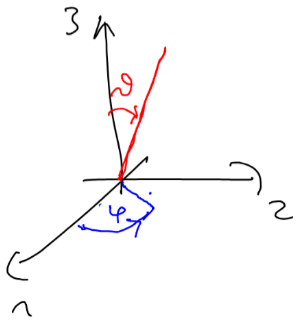
\includegraphics[width=0.5\linewidth]{figures/kugelkoordinaten}
      \label{fig:kugelkoordinaten}
    \end{figure}
    \( g \) ist zweimal stetig partiell differenzierbar.

    Sei \( f \) zweimal stetig differenzierbar auf \( \reals^3\to \reals \). \( \laplaceoperator f \) in Kugelkoordinaten bestimmen, also wenn wir \( \begin{pNiceMatrix} x \\ y \\ z \end{pNiceMatrix}=g(r,\theta,\phi) \)  schreiben. Zunächst überlegen wir, was es heißt, \( f  \) in Kugelkoordinaten zu schreiben.
    \begin{beispiel*}
      \( f(x,y,z)=xyz \).
      \begin{equation*}
        f\circ g(r,\theta,\phi)=f(r\Cos{\phi}\Sin{\theta},r\Sin{\phi}\Sin{\theta}, r\Cos{\theta})=r^3\sin^2\theta\Cos{\theta}\Cos{\phi}\Sin{\phi}\defines F(r,\theta,\phi).
      \end{equation*}
      Sodann:
      \begin{equation*}
        \totalderivative{g}(r,\theta,\phi)=\begin{pNiceMatrix}
          \Cos{\phi}\Sin{\theta}& r\Cos{\phi}\Cos{\theta} & -r\Sin \phi\Sin{\theta}\\
          \Sin{\phi}\Sin{\theta}& r\Sin{\phi}\Cos{\theta} & r\Cos{\phi}\Sin{\theta}\\
          \Cos{\theta} & -r\Sin{\theta}& 0
        \end{pNiceMatrix}
      \end{equation*}
      \( \Det \totalderivative{g}(r,\theta,\phi)=r^2\Sin{\theta}\) \timplies Ist \( \theta\neq k\pi \), \( k\in \wholes \), so ist \( g \) lokal umkehrbar mit stetig differenzierbarer Umkehrfunktion \( h\maps W\to V \) und in \( (x,y,z)\in W \) gilt
      \begin{align*}
        &f(\underbrace{x,y,z}_{=g(r,\theta,\phi)})=f\circ g\circ h(x,y,z)\defines F\circ h(x,y,z)\\
        \implies &\totalderivative{f}(x,y,z)=\explain{DF(r,\theta,\phi)}{\text{\( 1\times 3 \)-Matrix}}\matrixmult \overset{\underset{\downarrow}{\text{\( 3\times 3 \)-Matrix}}}{\underbrace{\totalderivative{h}(x,y,z)}_{=\inverse{\totalderivative{g}(r,\theta,\phi)}}}\defines \explain{\text{\( 1\times 3 \)-Matrix}}{\tilde{F}(r,\phi,\theta)}=\tilde{F}\circ h(x,y,z)\\
        \implies &(\partial_1^2+\partial_2^2+\partial_3^2)f(x,y,z)\begin{aligned}[t]
          &=\partial_1(\tilde{F}\circ h)_1 (\underbrace{x,y,z}_{\defines x})+\partial_2(\tilde{F}\circ h)_2 (x,y,z)+\partial_3(\tilde{F}\circ h)_3 (x,y,z)\\
          &=\sum_{j=1}^{3}(\partial_j \cdot \tilde{F}_j)(\underbrace{h(x)}_{\mathclap{=(r,\phi,\theta)}})\cdot\underbrace{\partial_j h_j(x)}_{\phantom{\partial_j g_j(r,\phi,\theta)}=\frac{1}{\partial_j g_j(r,\phi,\theta)}} \qquad (\text{Umkehrsatz})\\
          &=\sum_{j=1}^{3}\partial_j \tilde{F}_j(r,\theta,\phi)\cdot\frac{1}{\partial_j g_j(r,\phi,\theta)}.
        \end{aligned}
      \end{align*}
      Eine etwas längere Rechnung, bei der man \ua \( \totalderivative{g}(r,\theta,\phi) \) invertieren muss, liefert die explizite Formel für die \( \tilde{F}_j \), etwa
      \begin{equation*}
        \tilde{F}_1=\begin{pNiceMatrix} \partial_1 F & \partial_2 F & \partial_3 F \end{pNiceMatrix}\matrixmult\explain{\text{1.\ Spalte von \( \inverse{\totalderivative{g}(r,\theta,\phi)} \)}}{\begin{pNiceMatrix} \Cos{\phi}\Sin{\theta}\\ \frac{1}{r}\Cos{\phi}\Sin{\theta}\\ -\frac{1}{r}\frac{\Sin{\phi}}{\Sin{\theta}} \end{pNiceMatrix}}.
      \end{equation*}
      Von diesen berechnet man die jeweilige partielle Ableitung \( \partial_j \tilde{F}_j \) und multipliziert mit \( \frac{1}{\partial_j g_j} \).

      \zb
      \begin{align*}
        \partial_1 \tilde{F}_1&=\partial_1^2 F\cdot\Cos{\phi}\in \theta+\partial_1 \partial_2 \cdot\frac{1}{r}\Cos{\phi}\Cos{\theta}-\partial_2 F\cdot \frac{1}{r^2}\Cos{\phi}\Cos{\theta}-\partial_1 \partial_3 \cdot\frac{1}{r}\frac{\Sin{\phi}}{\Sin{\theta}}+\partial_3 F\frac{1}{r^2}\frac{\Sin{\phi}}{\Sin{\theta}}\\
        \quot{1}{\partial_1 g_1}&=\frac{1}{\Cos{\phi}\Sin{\theta}}.
      \end{align*}
      Das Ergebnis ist
      \begin{equation*}
        \frac{1}{r^2}\underset{=\partial_1}{\partial_r}(r^2\underset{=\partial_1}{\partial_r}F)+\frac{1}{r^2\Sin{\theta}}\underset{=\partial_2}{\partial_{\theta}}(\Sin{\theta}\underset{=\partial_2}{\partial_{\theta}} F)+\frac{1}{r^2\sin^2\theta}\underset{=\partial_3^2}{\partial_{\phi}^2}F.
      \end{equation*}
    \end{beispiel*}
  \end{enumerate}
\end{beispiele*}
\begin{ergaenzung*}
  \begin{figure}[H]
    \centering
    \includegraphics[width=0.9\linewidth]{lagrange_multiplikatoren_intuition}
    \label{fig:lagrange_multiplikatoren_intuition}
  \end{figure}
  Tatsache: \( \grad{h}(x,y) \) steht senkrecht auf \( h(x,y)=c \). (Der Gradient zeigt in die Richtung des stärksten Anstiegs der Funktion).
  \begin{figure}[H]
    \centering
    \includegraphics[width=0.9\linewidth]{lagrange_multiplikatoren_weitere_intuition}
    \label{fig:lagrange_multiplikatoren_weitere_intuition}
  \end{figure}
  Tatsache 2: Liegt in \( (x_0,y_0)\in \set{(x,y)|g(x,y)=0} \) ein Extremum von \( f \), so \texists \( \lambda\in \reals \) \sd \(\boxed{ \grad{f}(x_0,y_0)\lambda\grad{g}(x_0,y_0) }\). Tatsache 1 + 2 gleichbedeutend \( f(x,y)=c \) schmiegt sich in \( (x_0,y_0,) \) tangential an \( \set{g(x,y)=0} \) an.

  Das heißt, wenn wir das Gleichungssystem
  \begin{equation*}
    \left.\begin{aligned}
      \grad{f}(x,y)-\lambda\grad{g}(x,y&)=0\\
      g(x,y)&=0
    \end{aligned}\right\}\tag{\( * \)}\label{eq:lagrange_multiplikatoren_intuition}
  \end{equation*}
  lösen, haben wir Kandidaten für Extremstellen gefunden.
  \begin{align*}
    \eqref{eq:lagrange_multiplikatoren_intuition}\therefore \begin{aligned}[t]
      \partial_x L&=0\\
      \partial_y L&=0\\
      \partial_{\lambda} L&=0,
    \end{aligned}
  \end{align*}
  \( L \) Lagrange-Funktion.
\end{ergaenzung*}

% !TEX root = ./Vorlesungsmitschrift DIFF 2.tex  
\lecture{Mo 25.05. 10:15}{}
\section*{Taylor-Formel, lokale Extrema}
\begin{notation}[Multi-Index-Schreibweise]
  Sei \( \alpha\definedas(\alpha_1,\dotsc,\alpha_n)\in \naturals_{0}^n \). Dann definiert man
  \begin{align*}
    \abs{\alpha}&\definedas\alpha_1+\alpha_2+\dotsb+\alpha_n\\
    \Factorial{\alpha}&\definedas \Factorial{\alpha_1}\Factorial{\alpha_2}\dotsb\Factorial{\alpha_n}.
  \end{align*}
  Ist \( x=\transpose{(x_1,\dotsc,x_n)}\in \reals^n \), so setzt man 
  \begin{equation*}
    x^{a}\definedas x_1^{\alpha_1}x_2^{\alpha_2}\dotsb x_n^{\alpha_n}.
  \end{equation*}
  Ist \( f \) eine \( \abs{\alpha} \)-mal stetig differenzierbare Funktion, so ist 
  \begin{equation*}
    \partial^{\alpha}f\definedas \partial_1^{\alpha_1}\partial_2^{\alpha_2}\dotsb\partial_n^{\alpha_n}f
  \end{equation*}
\end{notation}
\begin{lemma}\label{funktion_entlang_gerade_ableitung}
  Sei \( f\maps U\to \reals \), \( U\subset \reals^n \) offen, ine \( k \)-fach stetig differenzierbare Funktion. Sei \( a\in U \) und sei \( h\in \reals^n \) so, dass \( \set{a+th|tt\in \interval{0}{1}} \) ganz in \( U \) liegt.
  \begin{figure}[H]
    \centering
    \includegraphics[width=0.5\linewidth]{verbindungsstrecke_in_umgebung}
    \label{fig:verbindungsstrecke_in_umgebung}
  \end{figure}
  Dann ist die Funktion \( g\maps \interval{0}{1}\to \reals \), \( g(t)=f(a+th) \) \( k \)-mal stetig differenzierbar und es gilt 
  \begin{equation*}
    g^{(k)}(t)=\sum_{\explain{\text{Summe über alle \( \alpha=(\alpha_1,\dotsc,\alpha_n)\in \naturals_0^h \) mit \( \alpha_1+\alpha_2+\dotsb+\alpha_n=k \)}}{\abs{\alpha}=k}}\frac{\Factorial{k}}{\Factorial{\alpha}}\partial^{\alpha}f(a+th)h^{\alpha}.
  \end{equation*}
\end{lemma}
\begin{proof}
  \begin{proofenumerate}
    \item Wir zeigen per Induktion über \( k \), dass gilt
    \begin{equation*}
      g^{(k)}(t)=\sum_{\mathclap{i_1,\dotsc,i_k\in \set{1,\dotsc,n}}}\partial_{i_1}\dotsb\partial_{i_k} f(a+th)h_{i_1}\dotsb h_{i_k}.
    \end{equation*}
    \begin{proofdescription}
      \item[Induktionsanfang: \( k=1 \)]
      \begin{align*}
        g'(t)&=Df(a+th)\matrixmult h\eqstep[p,v=false]{\text{Kettenregel}}\\
        &\sum_{i=1}^{n}\partial_i f(a+th) h_i.
      \end{align*}
      \item[\( k-1\to k \)]\Style{DDisplayFunc=outset}
      \begin{equation*}
        \D{\parens*{\sum_{i_1,\dotsc,i_{k-1}\in \set{1,\dotsc,n}}\partial_{i_1}\dotsb \partial_{i_{k-1}}f(a+th)h_{i_1}\dotsb h_{i_{k-1}}}}{t}=\sum_{i_1,\dotsc,i_{k-1}\in \set{1,\dots,n}} \sum_{i=1}^{n}\partial_i \partial_{i_1}\dotsc \partial_{i_{k-1}} f(a+th) h_{i_1}\dotsb h_{i_{k-1}}h_i.
      \end{equation*} 
    \end{proofdescription}
    \item Kommt unter den Indizes \( (i_1k,\dotsc,i_k) \) der Index \( 1 \) \( \alpha_1 \)-mal vor, der Index \( 2 \) \( \alpha_2 \)-mal,\dots, der Index \( n \) \( \alpha_n \)-mal, so ist 
    \begin{equation*}
      \partial_{i_1}\dotsb\partial_{i_k} f(a+th)=\partial_1^{\alpha_1}\dotsc \partial_n^{\alpha_n}f(a+th).
    \end{equation*}
    Es gibt 
    \begin{equation*}
      \frac{\Factorial{k}}{\Factorial{\alpha_1}\dotsb \Factorial{\alpha_n}}
    \end{equation*}
    \( k \)-Tupel \( (i_1,\dotsc,i_k) \) von Zahlen \( 1\leq i_j\leq n \), in denen \( 1 \) genau \( \alpha_1 \)-mal, \( 2 \) genau \( \alpha_2 \)-mal, \dots, \( n \) genau \( \alpha_n \)-mal vorkommt (ohne Beweis). \timplies \Beh.
  \end{proofenumerate}
\end{proof}
\begin{satz}[Taylorsche Formel]
  Sei \( f\maps U\to \reals \), \( U\subset \reals^n \) offen, \( (k+1) \)-mal stetig differenzierbar. Sei \( a\in U \) und \( h\in \reals^n \) \sd \( \set{a+tht|t\in \interval{0}{1}}\subset U \). Dann existiert \( \theta\in \interval{0}{1} \) \sd
  \begin{equation*}
    f(a+h)=\sum_{\substack{\abs{\alpha}\leq k\\ \alpha\in \naturals_0^n}}\frac{1}{\Factorial{\alpha}} \partial^{\alpha} f(a) h^{\alpha} +\sum_{\substack{\abs{\alpha}=k+1\\ \alpha\in \naturals_0^{n}}} \frac{1}{\Factorial{\alpha}} \partial^{\alpha} f(a+\theta h) h^{\alpha}.
  \end{equation*}
\end{satz}
\begin{proof}
  Setze \( g\maps \interval{0}{1}\to \reals \), \( g(t)\definedas f(a+th) \). Taylorsche Formel aus der \diff{1} \timplies \texists \( \theta\in \interval{0}{1} \) \sd
  \begin{equation*}
    g(1)=\sum_{j=0}^{k}\equalto{(\ref{funktion_entlang_gerade_ableitung})\logicspace \sum_{\abs{\alpha}=j}\frac{1}{\Factorial{\alpha}}\partial^{\alpha}f(a)h^{\alpha}}{\underbrace{\frac{1}{\Factorial{j}}g^{(j)}(0)}}+\equalto[Big]{\sum_{\abs{\alpha}=k+1}\frac{1}{\Factorial{\alpha}}f(a+\theta h)h^{\alpha}}{\underbrace{\frac{1}{\Factorial{(k+1)}}g^{(k+1)}(\theta)}}.
  \end{equation*}
\end{proof}
\begin{folgerung}
  Sei \( f\maps U\to \reals \), \( U\subset \reals^n \) offen, \( k \)-mal stetig differenzierbar. Sei \( a\in U \) und \( \delta>0 \) \sd \( B_{\delta}(a)\subset U \). Dann gilt für alle \( h\in B_{\delta}(0) \):
  \begin{equation*}
    f(a+h)=\sum_{\alpha\leq k}\frac{1}{\Factorial{\alpha}} \partial^{\alpha} f(a) h^{\alpha}+ R_{k,a}(h)
  \end{equation*}
  mit \( \frac{R_{k,a}(h)}{\norm{h}^k}\goesto 0 \) für \( h\goesto 0 \). 

  Äquivalent:
  \begin{equation*}
    f(x)=\sum_{\alpha\leq k}\frac{1}{\Factorial{\alpha}} \partial^{\alpha} f(a) (x-a)^{\alpha}+ R_{k,a}(x-a)
  \end{equation*}
  für \( x\in B_{\delta}(a)\). \emph{\enquote{Taylor-Entwicklung bis zur Ordnung \( k \) mit Entwicklungspunkt \( a \)}}.
\end{folgerung}
\begin{proof}
  \texists \( \theta=\alpha_{a,h}\in \interval{0}{1} \) \sd
  \begin{align*}
    f(a+h)&=\sum_{\abs{\alpha}\leq k-1}\frac{1}{\Factorial{\alpha}} f(a) h^{\alpha}+\sum_{\abs{\alpha}}\partial^{\alpha} f(a+\theta h)h^{\alpha}\\
    &=\sum_{\abs{\alpha}\leq k}\frac{1}{\Factorial{\alpha}} \partial^{\alpha}f(a) h^{\alpha}+\sum_{\abs{\alpha}=k}\frac{1}{\Factorial{\alpha}}\parens{\underbrace{\partial^{\alpha}f(a+\theta h)-\partial^{\alpha}f(a)}_{\definedas r_{\alpha,a}(h)}}h^{\alpha}.
  \end{align*}
  \( \partial^{\alpha} f \) ist stetig \timplies \( r_{\alpha,a}(h)\goesto r_{\alpha,a}(0)=0 \) für \( h\goesto 0 \) für \( h\goesto 0 \). Setze 
  \begin{equation*}
    R_{k,a}(h)\definedas \sum_{\abs{\alpha}=k}\frac{1}{\Factorial{\alpha}} r_{\alpha,a}(h) h^{\alpha},
  \end{equation*}
  dann gilt \( \frac{R_{k,\alpha}(h)}{\norm{h}^k}\goesto 0 \), denn
  \begin{equation*}
    \frac{\abs{h^\alpha}}{\explicitnorm{\max}{h}^k}=\frac{\abs{h_1}^{\alpha_1}\dotsb \abs{h_n}^{\alpha_n}}{\parens*{\explicitnorm{\max}{h}}^k}\leq 1
  \end{equation*}
  für \( \abs{\alpha}=\alpha_1+\dotsb+\alpha_n=k \).
  
\end{proof}

\begin{notation*}
  \begin{equation*}
    P_m(h)\definedas P_{m,a}(h)=\sum_{\abs{\alpha}=m}\frac{1}{\Factorial{\alpha}} \partial^{\alpha} f(a) h^{\alpha}
  \end{equation*}
  ist ein homogenes Polynom von Grad \( m \) (in \( h \)), das sogenannte \emph{Taylorpolynom} zu \( f \) zum Entwicklungspunkt \( a \). Es gilt
  \begin{equation*}
    f(a+h)=\sum_{m=0}^k P_{m,a}(h)+R_{k,a}(h).
  \end{equation*}
\end{notation*}
\begin{description}
  \item[\( m=0 \)] \( P_0(h)=f(a)\) konstant.
  \item[\( m=1 \)] Die Summe läuft über alle
  \begin{equation*}
    (\alpha_1,\dotsc,\alpha_n)\in \Set{(1,0,\dotsc,0),(0,1,0,\dotsc),\dotsc,(0,\dotsc,0,1)}.
  \end{equation*}
  Also gilt
  \begin{equation*}
    P_1(h)=\sum_{j=1}^{a} \partial_j f(a) h_j=\begin{pNiceMatrix} \partial_1 f(a) & \Cdots & \partial_n f(a) \end{pNiceMatrix}\matrixmult h.
  \end{equation*}
  Die Formel aus der Folgerung entspricht also genau der linearen Approximation von \( f \), die durch Ableitung gegeben ist.
  \item[\( m=2 \)] Die Summe läuft über alle
  \begin{multline*}
    (\alpha_1,\alpha_2,\dotsc,\alpha_n)\in\{ (1,1,0,\dotsc,0),(1,0,1,0,\dotsc,0),\dotsc\\
    ,(0,1,1,0,\dotsc,0),(0,1,0,1,0,\dotsc,0),\dotsc\\
    ,\dotsc\\
    ,(2,0,\dotsc,0),(0,2,0,\dotsc,0),\dotsc,(0,\dotsc,0,2)\}.
  \end{multline*}
  Also ist
  \begin{equation*}
    P_2(h)=\underbrace{\sum_{j=1}^{n}\sum_{i=j+1}^{n}\partial_i \partial_j f(a) h_i h_j}_{\mathclap{=\sum_{j<i}\partial_i \partial_j f(a) h_i h_j\explain{\text{\hyperlink{schwarzscher_satz}{Schwarz}}}{=}\frac{1}{2}\sum_{i\neq j}\partial_i \partial_j f(a) h_i h_j}}+\sum_{j=1}^n\frac{1}{2}\partial_j^2 f(a) h_j^2=\frac{1}{2}\sum_{i,j}\partial_j \partial_i f(a) h_i h_j.
  \end{equation*}
  Man definiert daher die sogenannte \emph{Hesse-Matrix}
  \begin{equation*}
    H_f(a)\definedas \parens*(\partial_i \partial_j f(a))_{\substack{i\in \set{1,\dotsc,n}\\j\in \set{1,\dotsc,n}}}
  \end{equation*}
  und schreibt
  \begin{equation*}
    \boxed{f(a+h)=f(a)+\scalarproduct{\grad f(a)}{h}+\frac{1}{2}\scalarproduct{h}{H_f(a) h}}+R_{z,a}(h)
  \end{equation*}
  für \( f\maps U\to \reals \) zweimal stetig differenzierbar und \( h\in B_{\delta}(0) \), \( \delta>0 \) \sd \( B_{\delta}(a)\subset U \).
\end{description}
\section*{Lokale Extrema}
Wir hatten in \ref{extremum_notwendige_bedingung} bereits gesehen: Ist \( a\in U \) lokale Extremstell von \( f\maps U\to \reals \), \( U\subset \reals^n \) offen, differenzierbar, so ist \( \grad f(a)=0 \).
\begin{satz}\label{hinreichende_bedingung_isoliertes_extremum}
  Sei \( f\maps U\to \reals \) zweimal stetig differenzierbar, \( U\subset \reals^n \) offen. Sei \( a\in U \) \sd \( \grad f(a)=0 \). Dann gilt:
  \begin{eigenschaftenenumerate}
    \item\label{hinreichende_bedingung_isoliertes_minimum} Ist \( H_f(a) \) positiv definit (\dh \( \scalarproduct{h}{H_f(a)h}>0 \) \tforall \( h\in \reals^n \), \( h\neq 0 \)), so hat \( f \) in \( a \) ein lokales (isoliertes) Minimum.
    \item\label{hinreichende_bedingung_isoliertes_maximum} Ist \( H_f(a) \) negativ definit (\dh \( \scalarproduct{h}{H_f(a)}<0 \) \tforall \( h\neq 0 \)), so hat \( f \) in \( a \) ein lokales (isoliertes) Maximum.
    \item\label{hinreichende_bedingung_kein_extremum} Ist \( H_f(a) \) indefinit (\dh \texists  \( h \) \sd \( \scalarproduct{h}{H_f(a)h}>0 \) \emph{und} \texists \( \tilde{h} \) \sd \( \scalarproduct{\tilde{h}}{H_f(a)\tilde{h}}<0 \)), so hat \( f \) in \( a \) kein lokales Extremum.
  \end{eigenschaftenenumerate}
\end{satz}
\begin{bemerkung*}
  Ist \( H_f(a) \) positiv oder negativ \emph{semi}definit \sd \tforall \( h\neq 0 \) ist \( \scalarproduct{h}{H_f(a)h}\geq 0 \) (\bzw \( \leq 0 \)), so ist keine allgemeine Aussage möglich.
\end{bemerkung*}
\begin{beispiel*}
  \( f_1(x,y)=x^2+y^4 \), \( f_2(x,y)=x^2 \), \( f_3(x,y)=x^2+y^3 \), \( H_{f_j}(0)=\begin{pNiceMatrix} 2 & 0 \\ 0 & 0 \end{pNiceMatrix} \) \tforall \( j \) ist positiv semidefinit (\( \scalarproduct{h}{H_{f_j}(0)h}=2h_1^2\geq 0 \), \( =0 \) für \( h_1=0 \)).
  \begin{figure}[H]
    \centering
    \begin{subfigure}[b]{0.3\textwidth}
      \centering
      \includegraphics[width=0.9\textwidth]{hesse_semi_definit_funktion_minimum}
      \caption*{\( 0 \) Minimalstelle}
    \end{subfigure}
    \begin{subfigure}[b]{0.3\textwidth}
      \centering
      \includegraphics[width=0.9\textwidth]{hesse_semi_definit_funktion_kein_isoliertes_minimum}
      \caption*{\( 0 \) nicht isolierte Minimalstelle}
    \end{subfigure}
    \begin{subfigure}[b]{0.3\textwidth}
      \centering
      \includegraphics[width=0.9\textwidth]{hesse_semi_definit_funktion_kein_extremum}
      \caption*{\( 0 \) ist keine Extremstelle}
    \end{subfigure}
    \caption{Wolfram Alpha}
  \end{figure}
\end{beispiel*}
\begin{proof}[Beweis von \ref{hinreichende_bedingung_isoliertes_extremum}]
  Setze \( A\definedas H_f(a) \). \texists \( \delta>0 \) \sd \( B_\delta(a)\subset U \). Und somit
  \begin{equation*}
    f(a+h)=f(a)+\scalarproduct{\underbrace{\grad f(a)}_{=0}}{h}+\frac{1}{2}\scalarproduct{h}{Ah}+R_2(h)\quad \forall h\in B_\delta(0)
  \end{equation*}
  mit \( \frac{R_2(h)}{\norm{h}^2}\goesto 0 \) (\( h\goesto 0 \)).
  \begin{equation*}
    \implies \forall \varepsilon>0 \logicspace \exists \tilde{\delta}>0\logicspace (\tilde{\delta}<\delta) \logicspace \text{\sd} \logicspace \abs{R_2(h)}\leq \varepsilon \norm{h}^2\quad \forall h\in B_{\tilde{\delta}}(0)
  \end{equation*}
  \begin{proofdescription}
    \item[\ref{hinreichende_bedingung_isoliertes_minimum}] Sei \( A \) positiv definit. Betrachte \( S=\set{h\in \reals^n|\euclidiannorm{h}=1} \). \( S \) ist abgeschlossen und beschränkt \( \subset \reals^n \) \timplies \( S \) ist kompakt \timplies \( S\ni h\mapsto \scalarproduct{h}{Ah} \) nimmt Maximum und Minimum an (da stetig).
    \begin{equation*}
      \alpha\definedas \inf_{h\in S}\underbrace{\scalarproduct{h}{Ah}}_{\mathclap{>0\logicspace  (\text{VOR})\logicspace (h\neq 0 \text{ wenn }h\in S)}}>0.
    \end{equation*}
    \begin{behauptung*}
      \begin{equation*}
        \scalarproduct{h}{Ah}\geq \alpha\euclidiannorm{h}^2 \quad \forall h\in \reals^n.
      \end{equation*}
    \end{behauptung*}
    \begin{subproof}
      \( h=0\): \checkmark. Sei also \( h\neq 0 \). Setze \( \tilde{h}\definedas\frac{1}{\euclidiannorm{h}}h \).  
      \begin{equation*}
        \implies \tilde{h}\in S\implies \scalarproduct{\tilde{h}}{A\tilde{h}}\geq \alpha.
      \end{equation*}
      Die Behauptung folgt wegen
      \begin{equation*}
        \scalarproduct{\tilde{h}}{A\tilde{h}}=\frac{1}{\euclidiannorm{h}^2}\scalarproduct{h}{Ah}.
      \end{equation*}
    \end{subproof}
    Wähle nun \( \tilde{\delta}>0 \) \sd \( \abs{R_2(h)}\leq \frac{\alpha}{4}\euclidiannorm{h}^2 \) für \( \norm{h}<\tilde{\delta} \).
    \begin{equation*}
      \implies f(a+h)\geq f(a)+\frac{1}{2}\underbrace{\scalarproduct{h}{Ah}}_{\geq \alpha\euclidiannorm{h}^2}-\abs{R_2(h)}\geq f(a)+\underbrace{\frac{1}{4}\alpha\euclidiannorm{h}^2}_{\geq 0}>f(a)\quad \forall \norm{h}<\tilde{\delta},\logicspace  h\neq 0.
    \end{equation*}
    \item[\ref{hinreichende_bedingung_isoliertes_maximum}] Ist \( A \) negativ definit, betrachte \( -f \) und wende \ref{hinreichende_bedingung_isoliertes_minimum} an.
    \item[\ref{hinreichende_bedingung_kein_extremum}] Ist \( A \) indefinit, gibt es in jeder Umgebung \( V \) von \( a \) Punkte \( x,x'\in V \) \sd 
    \begin{equation*}
      f(x)<f(a)<f'(x).
    \end{equation*}
    Es gilt \( v\in \reals^n \), \sd \( \scalarproduct{v}{Av}\defines \alpha >0 \).
    \begin{equation*}
      \implies f(a+th)= f(a)+\frac{1}{2}t^2 a+R_2(tv)
    \end{equation*}
    für \( \abs{t} \) klein genug (\sd \( tv\in B_{\delta}(0) \)). Wähle \( \abs{t}>0 \) so klein, dass zudem \( R_2(tv)\leq \frac{\alpha}{2}t^2 \)
    \begin{equation*}
      \implies f(a+sv)\geq f(a)+\frac{1}{2}s^2\alpha-\abs{R_2(sv)}>f(a)
    \end{equation*}
    für \( 0<s<t \) (\obda \( t>0 \)). 
    
    Genauso: Es gibt \( v\in \reals^n \), \sd \( \scalarproduct{v}{Av}\defines \alpha<0 \)
    \begin{equation*}
      \implies f(x+tv)=f(x)-\frac{1}{2}t^2\abs{\alpha}+R_2(tv)
    \end{equation*}
    für \( \abs{t} \) klein genug (\sd \( tv\in B_{\delta}(0) \)). Wähle \( \abs{t}>0 \) so klein, dass zudem \( \abs{R_2(tv)}\leq\frac{\alpha}{4}t^2 \)
    \begin{equation*}
      \implies f(a+sv)\leq f(a)-\frac{1}{2}s^2\abs{\alpha}+\abs{R_2(sv)}<f(a)\quad \forall 0<s<t\quad (\text{\obda }t>0).
    \end{equation*}
  \end{proofdescription}
\end{proof}
\begin{beispiele*}
  \begin{enumerate}
    \item \( f\maps \reals^2\to \reals \), \( f(x)=x_1^2+x_2^2+2 \), \(\grad f(a)=(2a_1,2a_2)=0\) nur für \( a=0 \).
    \begin{equation*}
      H_f(0)=\begin{pNiceMatrix} 2 & 0 \\ 0 & 2 \end{pNiceMatrix}
    \end{equation*} positiv definit \timplies isoliertes Minimum in \( 0 \).  
    \item \( f\maps \reals^2\to \reals \), \( f(x)=2-x_1^2-x_2^2 \), \( \grad f(a)=-2a=0 \) nur für \( a=0 \). 
    \begin{equation*}
      H_f(0)=\begin{pNiceMatrix} -2 & 0 \\ 0 & -2 \end{pNiceMatrix}
    \end{equation*}
    negativ definit \timplies isoliertes Maximum in \( 0 \).
    \item \( f\maps \reals^2\to \reals \), \( f(x)=2+x_1^2-x_2^2 \), \( \grad f(a)=2a_1-2a_2=0 \) nur für \( a=0 \).
    \begin{equation*}
      H_f(0)=\begin{pNiceMatrix} 2 & 0 \\ 0 & -2 \end{pNiceMatrix}
    \end{equation*}
    indefinit:
    \begin{gather*}
      \textcolor{blue}{\scalarproduct{e_1}{H_f(0)e_1}}=2=-\textcolor{red}{\scalarproduct{e_2}{H_f(0)e_2}}\\
      \textcolor{blue}{f(0+te_1)>f(0)\quad \forall t\neq 0}\\
      \textcolor{red}{f(0+te_2)<f(0)\quad \forall t\neq 0}.
    \end{gather*}
    \begin{figure}[H]
      \centering
      \includegraphics[width=0.5\linewidth]{hesse_indefinit_funktion_sattelflaeche}
      \caption*{Sattelfläche}
      \label{fig:hesse_indefinit_funktion_sattelflaeche}
    \end{figure}
  \end{enumerate}
\end{beispiele*}
\begin{bemerkung*}
  Wie untersucht man in komplizierten Fällen \( H_f(a) \) auf Definitheit? Kennt man die Eigenwerte (\texists wegen Symmetrie!) ist klar: Sind all positiv (negativ), so ist \( H_f(a) \) positiv (negativ) definit, gibt es positive und negative Eigenwerte, so ist sie indefinit. Aber Eigenwerte großer Matrizen sind schwer zu bestimen. Besser geeignet ist
\end{bemerkung*}
\begin{lemma}[aus der AGLA\@: Kriterium von Hurwitz]
  Sei \( A\in \sqmatrices{n}{\reals} \) symmetrisch. Dann ist \( A \) genau dann positiv definit, wenn
  \begin{equation*}
    \Det \explain{\text{Haupt-Minoren von \( A \)}}{\begin{pNiceMatrix} A_{11} & \Cdots & A_{1k} \\ \Vdots &  & \Vdots \\ A_{k1} & \Cdots & A_{kk} \end{pNiceMatrix}}>0\quad \forall k\in \set{1,\dotsc,n}
  \end{equation*}
  und genau dann negativ definit, wenn
  \begin{align*}
    \Det(A_{11})=A_{11}&<0\\
    \Det \begin{pNiceMatrix} A_{11} & A_{12} \\ A_{21} & A_{22} \end{pNiceMatrix}&>0
  \end{align*}
  und dann immer abwechselnd.
\end{lemma}

% !TEX root = ./Vorlesungsmitschrift DIFF 2.tex  
\chapter{Untermannigfaltigkeiten des \texorpdfstring{\( \reals^n \)}{R\^n}}
\lecture{Do  28.05. 10:15}{}
Ziel (\ua) Geometrische Interpretation der Ableitung.
\begin{erinnerung*}
  Der Gradient zeigt in die Richtung des stärksten Anstiegs.
  \begin{figure}[H]
    \centering
    \includegraphics[width=0.8\linewidth]{erinnerung_gradient_intuition}
    \caption*{}
    \label{fig:erinnerung_gradient_intuition}
  \end{figure}
  In einem Beispiel hatten wir gesehen: Richtungsableitung in Richtung einer Niveaufläche steht \( \perp \) auf \( \grad-{f} \).
  \begin{figure}[H]
    \centering
    \includegraphics[width=0.8\linewidth]{erinnerung_niveauflaeche_intuition}
    \label{fig:erinnerung_niveauflaeche_intuition}
  \end{figure}
  Satz über implizite Funktion: 
  \begin{figure}[H]
    \centering
    \includegraphics[width=0.5\linewidth]{satz_implizite_funktion_erinnerung_intuition}
    \caption*{\( f\maps U_1\times U_2 \to \reals \). Niveaumenge kann lokal als Graph geschrieben werden, wenn \( D_2 f(a,b) \) invertierbar ist. \textcolor{red}{Weitere Erklärungen \tto Audio}.}
    \label{fig:satz_implizite_funktion_erinnerung_intuition}
  \end{figure}
\end{erinnerung*}
\begin{aufwaermuebung*}
  Sei \( \gamma\maps I\to \reals^3 \) differenzierbare Kurve.
  \begin{figure}[H]
    \centering
    \includegraphics[width=0.5\linewidth]{spur_einer_kurve_auf_mannigfaltigkeit}
    \label{fig:spur_einer_kurve_auf_mannigfaltigkeit}
  \end{figure}
  Dann ist \( \gamma'(t) \) der \emph{Geschwindigkeitsvektor}, der sich im Punkt \( \gamma(t) \) auf die Kurve schmiegt.
\end{aufwaermuebung*}
\begin{beispiel*}
  \( f\maps I\to \reals \) differenzierbare Funktion. Betrachte \( \gamma(t)\definedas (t,f(t)) \). Also Spur von \( \gamma=\Gamma_f \). \( \gamma'(t)=(1,f'(t)) \).
  \begin{figure}[H]
    \centering
    \includegraphics[width=0.5\linewidth]{graph_als_kurve_auf_mannigfaltigkeit}
    \label{fig:graph_als_kurve_auf_mannigfaltigkeit}
  \end{figure}
\end{beispiel*}
\begin{definition}\label{untermannigfaltigkeit}\index{Untermannigfaltigkeit}
  Eine Teilmenge \( M\subset \reals^n \) heißt \( d \)-dimensionale differenzierbare \emph{Unter-Mannigfaltigkeit} (oder reguläre Fläche) des \( \reals^n \), falls es für jedes \( a\in M \) eine Umgebung \( U\subset \reals^n \) von \( a \) gibt und eine stetig differenzierbare Abbildung \( f\maps U\to \reals^{n-d} \) \sd \begin{eigenschaftenenumerate}
    \item \label{untermannigfaltigkeit:ist_niveaumenge}\( M\cap U=\set{x\in U|f(x)=0} \) und 
    \item \label{untermannigfaltigkeit:maximaler_rang_gibt_dimension} \( \rang-{Df(a)}=n-d \) (maximal).
  \end{eigenschaftenenumerate}
  Das heißt \( M \) lässt sic lokal als Nullstellengebilde von \( n-d \) \( \reals \)-wertigen \( \stetigefunktionen[1] \) Funktionen \( f_j \) schreiben, deren Gradienten linear unabhängig sind.
  \begin{figure}[H]
    \centering
    \includegraphics[width=0.5\linewidth]{untermannigfaltigkeit_intuition}
    \label{fig:untermannigfaltigkeit_intuition}
  \end{figure}
\end{definition}
\begin{beispiele*}
  \begin{enumerate}
    \item \label{untermannigfaltigkeit:beispiele:maximale_dimension:offene_teilmengen}Die \( n \)-dimensionalen Untermannigfaltigkeiten des \( \reals^n \) sind die offenen Teilmengen. Hier ist
    \begin{equation*}
      M\cap U=U=\Set{x\in U}.
    \end{equation*}
    \item\label{untermannigfaltigkeit:beispiele:ebene_4d} Ebene
    \begin{equation*}
      E=\set{p+(s,t,0,0)|s,t\in \reals}\subset \reals^4,
    \end{equation*}
    \( p\in \reals^4 \).
    \begin{figure}[H]
      \centering
      \includegraphics[width=0.5\linewidth]{langweilige_ebene_als_untermannigfaltigkeit}
      \caption*{Eine Dimension im Bild unterdrückt.}
      \label{fig:langweilige_ebene_als_untermannigfaltigkeit}
    \end{figure}
    Zu \( a\in E \) wähle \( U=\reals^4 \) und setze
    \begin{align*}
      f_1&\maps U\to \reals & f_1(x)&=\scalarproduct{x-p}{e_3}=x_3-p_3\\
      f_1&\maps U\to \reals & f_1(x)&=\scalarproduct{x-p}{e_4}=x_4-p_4.
    \end{align*}
    Es gilt \( x\in E \) \tiff \( f(x)=\begin{pNiceMatrix} f_1(x) \\ f_2(x) \end{pNiceMatrix}=0 \) und \( Df(a)=\begin{pNiceMatrix}
      0 & 0 & 1 & 0 \\ 0 & 0 & 0 & 1
    \end{pNiceMatrix} \), \( \rang-{}=2 \).
    \begin{figure}[H]
      \centering
      \includegraphics[width=0.5\linewidth]{normalenvektor_auf_langweiliger_ebene_als_untermannigfaltigkeit}
      \label{fig:normalenvektor_auf_langweiliger_ebene_als_untermannigfaltigkeit}
      \begin{equation*}
        \grad-{f_1}(a)=\begin{pNiceMatrix} 0 \\ 0 \\ 1 \\ 0 \end{pNiceMatrix}\qquad \grad-{f_2}(a)=\begin{pNiceMatrix} 0 \\ 0 \\ 0 \\ 1 \end{pNiceMatrix}.
      \end{equation*}
    \end{figure}
    Niveau-Mengen von \( f \):
    \begin{equation*}
      N_f(c)=\Set{x\in \reals^n|x_3-p_3=c,\logicspace x_4-p_4=c}.
    \end{equation*}
    \begin{figure}[H]
      \centering
      \includegraphics[width=0.5\linewidth]{normalenvektor_auf_langweiliger_ebene_als_niveaumengen}
      \caption*{\( N_f(0)=E \), Gradient steht senkrecht.}
      \label{fig:normalenvektor_auf_langweiliger_ebene_als_niveaumengen}
    \end{figure}
    \item \label{untermannigfaltigkeit:beispiele:sphaere}\( \mathbb{S}^{n-1}\definedas \Set{x\in \reals^n|\euclidiannorm{x}=1} \). Einheits-Sphäre. Zu \( a\in \mathbb{S}^{n-1} \) wähle \( U=\reals^n \) und \( f(x)=\euclidiannorm{x}^2-1 \). 
    \begin{equation*}
      Df(a)=(2a_1,\dotsc,2a_n)\neq 0.,
    \end{equation*}
    also \( \rang-{}=1 \forall a\in \mathbb{S}^{n-1}\).
    \item Eine \( 1 \)-dimensionale differenzierbare Untermannigfaltigkeit wird auch unparametisierte differenzierbare Kurve genannt. 
    \begin{beispiel*}
      \( f\maps \reals^3\to \reals^2 \).
      \begin{equation*}
        f(x,y,z)=\begin{pNiceMatrix} x^2+y^2+z^2-R^2 \\ x^2+y^2-r^2 \end{pNiceMatrix}\qquad R>r>0.
      \end{equation*}
      \begin{figure}[H]
        \centering
        \includegraphics[width=0.5\linewidth]{zwei_kreise_auf_kugel_und_zylinder_als_untermannigfalteigkeit}
        \caption*{\textcolor{red}{\( M=\Set{(x,y,z)|f(x,y,z)=0}=N_f(0) \)}}
        \label{fig:zwei_kreise_auf_kugel_und_zylinder_als_untermannigfalteigkeit}
      \end{figure}
      \begin{equation*}
        Df(x,y,z)=\begin{pNiceMatrix} 2x & 2y & 2z \\ 2x & 2y & 0 \end{pNiceMatrix}
      \end{equation*}
      hat maximalen Rang \( 2 \) für \( z\neq 0 \) und \( (x,y)\neq 0 \).

      Letzteres ist für alle \( a\in M \) gewährleistet, weil \( (x^2+y^2=r^2>0) \) gilt und somit ist auch ersteres gewährleistet, da \( z^2=-r^2+R^2>0 \).

      Man sieht auch direkt: Die Funktion, die \( M \) lokal als Nullstellenmenge beschreibt, ist nicht eindeutig: \zb
      \begin{equation*}
        \tilde{f}(x,y,z)=\begin{pNiceMatrix} z^2+r^2-R^2 \\ x^2+y^2-r^2 \end{pNiceMatrix}
      \end{equation*}
      beschreibt im Beispiel oben das selbe \( M \).
    \end{beispiel*}
  \end{enumerate}
\end{beispiele*}
\begin{definition}\label{tangentialraum}\index{Tangentialvektor}
  Ein Vektor \( v\in \reals^n \) heißt \emph{Tangentialvektor} der Untermannigfaltigkeit \( M\subset \reals^n \) im Punkt \( a \), falls \texists differenzierbare Kurve \( \gamma \), \( \gamma\maps \ointerval{-\varepsilon}{\varepsilon} \to M\), \sd \( \gamma(0)=a \) und \( v=\gamma'(0) \). Die Menge der Tangentialvektoren im Punkt \( a \) bezeichnet man mit \( \tangentialraum-{M} \). 
  \begin{figure}[H]
    \centering
    \includegraphics[width=0.5\linewidth]{tangentenvektoren_intuition}
    \caption*{Man zeichnet Tangentialvektoren an den Punkt \( a \) an. Aber eigentlich sind es \emph{keine} affinen Vektoren.}
    \label{fig:tangentenvektoren_intuition}
  \end{figure}
\end{definition}
\begin{beispiele*}
  \begin{enumerate}
    \item Ebene
    \begin{equation*}
      E=\set{p+(s,t,0,0)|s,t\in \reals}\subset \reals^4,
    \end{equation*}
    \( p\in \reals^4 \), \( a\in E \).
    \begin{equation*}
      \tangentialraum-{M}=\Set{v\in \reals^4|v=v_1e_2+v_2e_2},
    \end{equation*}
    denn jedes \( \gamma\maps \ointerval{-\varepsilon}{\varepsilon}\to M \) mit \( \gamma(0) \) ist von der FOrm
    \begin{equation*}
      \gamma(t)=a+(\tilde{\gamma}_1(t),\tilde{\gamma}_2(t),0,0).
    \end{equation*}
    Man zeichnet den Tangentialraum an der Stelle \( a \) ein, also
    \begin{figure}[H]
      \centering
      \includegraphics[width=0.5\linewidth]{tangentialvektor_an_ebene}
      \label{fig:tangentialvektor_an_ebene}
    \end{figure}
    \item \( M=\mathbf{S}^{n-1} \). Behauptung: 
    \begin{figure}[H]
      \centering
      \includegraphics[width=0.5\linewidth]{tangentialraum_an_kugel}
      \label{fig:tangentialraum_an_kugel}
    \end{figure}
    Das erklärt den Namen: Die Tangentialvektoren sind tangential (angeschmiegt) an \( M \) im Punkt \( a \).
    
    Zum Beweis der Behauptung beweisen wir allgemeiner:
  \end{enumerate}
\end{beispiele*}
\begin{satz}\label{tangentialraum_ist_tangential}
  \approxtimestamp{24}
  Sei \( M \) \( d \)-dimensionale differenzierbare Untermannigfaltigkeit des \( \reals^n \). Ist 
  \begin{equation*}
    a\in M\cap U =\set{x\in U |f(x)=0}
  \end{equation*}
  für eine Funktion \( f\maps U\to \reals^{n-d} \) wie in \thref{untermannigfaltigkeit}, also \( Df(a) \) von maximalem Rang (\( n-d \)). Dann ist \( \tangentialraum-{M}=\ker-{Df(a)} \). Insbesondere ist \( \tangentialraum-{M} \) Untervektorraum von \( \reals^n \).
\end{satz}
\begin{proof}
  \begin{proofdescription}
    \item[\enquote{\( \subset \)}] Sei \( \gamma\maps \ointerval{-\varepsilon}{\varepsilon}\to M\cap U \) mit \( \gamma(0)=a \), \( \gamma'(0)=v \). Dann ist 
    \begin{equation*}
      0=\evaluateat{\frac{\differential}{\differential t} f\circ \gamma(t)}{t=0}=Df(\gamma(0))\matrixmult \gamma'(0)=Df(a)\matrixmult v\implies v\in \ker-{Df(a)}.
    \end{equation*}
    \item[\enquote{\( \supset \)}] Beweisen wir später mit Hilfe des folgenden Satzes~\ref{untermannigfaltigkeit_kriterium}.
  \end{proofdescription}  
\end{proof}
\begin{interpretation*}[für \( n-d=1 \)]
  Der Gradient zeigt in die Richtung des stärksten Anstiegs von \( f \). Eine Kurve \( \gamma \) wi in \ref{tangentialraum} (und \ref{tangentialraum_ist_tangential}) verläuft in einer Niveaumenge von \( f \) (und zwar hier zu \( c=0 \)). In Richtung \( v=\gamma'(0) \) ändert sich \( f \) also nicht und die Richtungsableitung in Richtung \( v \) ist \( 0 \):
  \begin{equation*}
    \partial_v f(a)=\scalarproduct{v}{\grad-{f}(a)}=Df(a)\matrixmult v=0\qquad (\text{\thref{tangentialraum_ist_tangential}}),
  \end{equation*}
  also \( v\perp \grad-{f}(a) \). \enquote{Der Gradient steht auf Niveaumengen senkrecht}.
\end{interpretation*}
\begin{beispiel*}
  \( f(x,y)=x^2+y^2-2 \). \( M= \) Niveaumenge \( N_f(0)=\set{x^2+y^2=2} \). \( \grad-{f}(a)=2(a_1,a_2) \).
  \begin{figure}[H]
    \centering
    \includegraphics[width=0.5\linewidth]{tangentialraum_an_kreis_ist_tangential}
    \label{fig:tangentialraum_an_kreis_ist_tangential}
  \end{figure}
  Eine Kurve, die in \( M \) verläuft und für die gilt
  \begin{equation*}
    \gamma(0)=a=\begin{pNiceMatrix} \sqrt{2} \\ 0 \end{pNiceMatrix} 
  \end{equation*}
  ist
  \begin{equation*}
    \gamma(t)=\begin{pNiceMatrix} \Cos{t} \\ \Sin{t} \end{pNiceMatrix}\cdot \sqrt{2}.
  \end{equation*}
  Es ist dann
  \begin{equation*}
    \gamma'(0)=\sqrt{2}\begin{pNiceMatrix} 0 \\ 1 \end{pNiceMatrix}\perp \grad-{f}\begin{pNiceMatrix} \sqrt{2} \\ 0 \end{pNiceMatrix}=\begin{pNiceMatrix} 2\sqrt{2} \\ 0 \end{pNiceMatrix}.
  \end{equation*}
  \minisec{Höher-dimensionale Sphären:}
  \( N_f(0) \), \( f(x)=\euclidiannorm{x}^2-1 \). \( Df(a)=2(a_1,\dotsc,a_n) \). \( \ker-{Df}(a)= \) Ebene senkrecht zu \( a \).
  \begin{figure}[H]
    \centering
    \includegraphics[width=0.5\linewidth]{tangentialraum_an_sphaere_ist_tangential}
    \label{fig:tangentialraum_an_sphaere_ist_tangential}
  \end{figure}
  Um di Rückrichtung von \thref{tangentialraum_ist_tangential} beweisen zu können, benötigen wir eine weitere (äquivalente) Charakterisierung differenzierbarer Untermannigfaltigkeiten.
\end{beispiel*}
\begin{satz}\label{untermannigfaltigkeit_kriterium}
  Eine Teilmenge \( M\subset \reals^n \) ist genau dann \( d \)-dimensionale differenzierbare Untermannigfaltigkeit des \( \reals^n \), wenn es zu jedem Punkt \( a\in M \) (nach eventueller Umnummerierung) Umgebungen \( V_1\subset \reals^d \) von \( a'=(a_1,\dotsc,a_d) \) un \( V_2\subset \reals^{n-d} \) von \( a''=(a_{d+1},\dotsc,a_n) \) und eine stetig differenzierbare Abbildung \( g\maps V_1\to \reals^{n-d} \), \( g(V_1)\subset V_2 \) gibt, \sd
  \begin{equation*}
    M\cap (V_1\times V_2)=\Gamma_g = \Set{(x',g(x'))|x'\in V_1}.
  \end{equation*}
\end{satz}
\begin{proof}
  \begin{proofdescription}
    \item[\hin] Sei \( a\in M \), \( U \), \( f \) wie in \thref{untermannigfaltigkeit}, insbesondere \( \rang-{Df(a)}=n-d \) (maximal) \timplies nach eventueller Umnummerierung ist \( Df(x',x'') \) für \( x=(x',x'')\in U\subset \reals^d \times\reals^{n-d} \)
    \begin{equation*}
      \begin{pNiceMatrix}[last-row]
        \partial_1 f_1(x' ,x'') & \Cdots & \partial_d f_1(x'.x'') & \partial_{d+1}f_1(x',x'')&\Cdots \partial_n f_1(x',x'') \\
        \Vdots &  & \Vdots & \Vdots & & \Vdots  \\
         \partial_1 f_{n-d}(x' ,x'') & \Cdots & \partial_d f_{n-d}(x'.x'') & \partial_{d+1}f_{n-d}(x',x'')&\Cdots \partial_n f_{n-d}(x',x'')\\
         &&&\Hdotsfor{3}_{D_2f(x'.x'')}
      \end{pNiceMatrix},
    \end{equation*}
    \sd \( D_2f(a',a'') \) invertierbar ist.

    Zudem ist \( f(a)=0 \). Der Satz über implizite Funktion liefert also eine lokale Auflösung von \( N_f(0) \) \timplies \Beh.

    \item[\rueck] Sei 
    \begin{equation*}
      M\cap V_1\times V_2=\Set{(x',g(x'))|x'\in V_1},
    \end{equation*}
    \( V_1\subset \reals^d \), \( V_2\subset \reals^{n-d} \). Setze
    \begin{gather*}
      f\maps V_1\times V_2\to \reals^{n-d}\\
      f_j(x',x'')=g_j(x')-x_j''.
    \end{gather*}
   Dann ist \end{proofdescription}  
   \begin{equation*}
     M\cap V_1\times V_2=\set{x\in V_1\times V_2|f(x)=0}
   \end{equation*}
   und
   \begin{equation*}
     Df(x)=\begin{pNiceArray}{CCC|CCC}[first-col]
       & \partial_1 g_1(x) & \Cdots & \partial_d g_1(x) & -1 & & 0 \\
       & \Vdots &  & \Vdots &  &\Ddots &  \\
       & \partial_1 g_{n-d}(x) & \Cdots & \partial_d g_{n-d}(x) & 0 & & -1 \\
     \end{pNiceArray}
   \end{equation*}
   hat maimalen Rang (\( n-d \)).
\end{proof}
\begin{bemerkung*}
  Man kann also eine \( d \)-dimensionale differenzierbare Untermannigfaltigkeit lokal stets als Graphen einer \( \stetigefunktionen[1] \)-FUnktion schreiben.

  Für die Beispiele oben gilt
  \begin{description}
    \item[\ref{untermannigfaltigkeit:beispiele:maximale_dimension:offene_teilmengen}] \( U\subset \reals^n \) offen, \( V_2=\emptyset \), \( V_1=U \).
    \item[\ref{untermannigfaltigkeit:beispiele:ebene_4d}] Ebene
    \begin{equation*}
      E=\set{p+s e_1+t e_2|s,t\in \reals}\subset \reals^4,
    \end{equation*}
    \( p\in \reals^4 \).
    \begin{equation*}
      g\maps \reals^2\to \reals^2\qquad g(x_1,x_2)=\begin{pNiceMatrix} p_3 \\ p_4 \end{pNiceMatrix}
    \end{equation*}
    konstant.
    \begin{figure}[H]
      \centering
      \includegraphics[width=0.5\linewidth]{langweilige_ebene_als_graph}
      \label{fig:langweilige_ebene_als_graph}
    \end{figure}
    \item[\ref{untermannigfaltigkeit:beispiele:sphaere}] \( \mathbf{S}^{n-1} \): Sei \( a\in \mathbf{S}^{n-1} \) mit \( a_n>0 \). Sei
    \begin{gather*}
      V_1=\Set{x'\in \reals^{n-1}|\euclidiannorm{x'}<1}\\
      g\maps V_1\to \reals,\qquad g(x_1,\dotsc,x_{n-1})=\sqrt{1-x_1^2--\dotsb-x_{n-1}^2}.
    \end{gather*}
    Dann ist
    \begin{equation*}
      \mathbf{S}^{n-1}\cap V_1\times \ointerval{0}{\infty}=\Gamma_g.
    \end{equation*}
    \begin{figure}[H]
      \centering
      \includegraphics[width=0.5\linewidth]{halbsphaere_als_graph}
      \label{fig:halbsphaere_als_graph}
    \end{figure}
  \end{description}
\end{bemerkung*}\approxtimestamp{40}
\begin{proof}[Fortsetzung Beweis \thref{tangentialraum_ist_tangential}]
  Wir beweisen nun die zweite Inklusion von \thref{tangentialraum_ist_tangential}, also \( \tangentialraum-{M}\supset \ker-{Df(a)} \). Sei \( g\maps V_1\to \reals^{n-d} \) stetig differenzierbar \sd \( g(V_1)\subset V_2 \) und \( a\in V_1\times V_2\subset \reals^d \times \reals^{n-d} \) und
\begin{equation*}
  M\cap (V_1\times V_2)=\Gamma_g=\Set{(x,g(x))|x\in V_1}.
\end{equation*}
Sei \( x_0\in V_1  \) \sd \( (x_0,g(x_0))=a \). Betrachte \( \varphi\maps V_1\to \reals^n \), \( \varphi(x)=(x,g(x)) \). Dann ist
\begin{equation*}
  D\varphi(x_0)\matrixmult v\explain{\text{Kettenregel}}{=}\evaluateat{\frac{\differential}{\differential t} \varphi(x_0+tv)}{t=0}\qquad \forall v\in \reals^d.
\end{equation*}
\timplies \( a=\varphi(x-0) \) und 
\begin{equation*}
  w\definedas \evaluateat{\frac{\differential}{\differential t} \varphi(x_0+tv)}{t=0}\in \tangentialraum-{M},
\end{equation*}
also \( \image{D\varphi(x_0)}\subset \tangentialraum-{M} \). Zudem wissen wir schon: \( \tangentialraum-{M}\subset \ker-{Df(a)} \). Es ist \( D\varphi(x_0)\maps \reals^d\to \reals^n \), \( D\varphi(x_0)=\begin{pNiceMatrix} \mathds{1}_{d\times d} \\ Dg(x_0) \end{pNiceMatrix} \), also injektiv \timplies (Dimensionsformel)
\begin{equation*}
  \dim-{\image{D\varphi(x_0)}}=d=n-\underbrace{\rang-{Df(a)}}_{=n-d}=\dim-{\ker-{Df(a)}}
\end{equation*}
\timplies \( \tangentialraum-{M}=\ker-{Df(a)} \).
\end{proof}
Wir haben im Beweis auch gesehen:
\begin{equation*}
  \tangentialraum-{M}=\image-{D\varphi(x_0)},
\end{equation*}
wo \( \phi(x)=\transpose-{(x,g(x))} \) die Graphenabbildung einer lokalen Auflösung \( g \) ist it \( a=\transpose-{(x_0,g(x_0))}=\phi(x_0) \).

Die geometrische Interpretation ist:
\begin{figure}[H]
  \centering
  \includegraphics[width=0.5\linewidth]{setup_interpretation_bild_ableitung_implizite_funktion}
  \label{fig:setup_interpretation_bild_ableitung_implizite_funktion}
\end{figure}
\begin{equation*}
  D\phi(x_0)=\explain{\partial_1 g(x_0)\logicspace  \partial_2 g(x_0)}{\begin{pNiceMatrix} \mathds{1}_2 \\ Dg(x_0) \end{pNiceMatrix}}.
\end{equation*}
Die Spalten von \( D\phi(x_0) \) 
\begin{equation*}
  \explain[Big]{\text{Veränderug von \( g \) in \( 1 \)-Richtung}}{\begin{pNiceMatrix} 1 \\ 0 \\ \partial_1 g(x_0) \end{pNiceMatrix}}\logicspace \text{und}\logicspace \explain{\text{Veränderung in \( 2 \)-Richtung}}{\begin{pNiceMatrix} 0 \\ 1 \\ \partial_2 g(x_0) \end{pNiceMatrix}}
\end{equation*}
\begin{figure}[H]
  \centering
  \includegraphics[width=0.5\linewidth]{interpretation_bild_ableitung_implizite_funktion}
  \caption*{\textcolor{green}{Ebene parallel zur \( 2 \)-\( 3 \)-Ebene durch \( a \)\( =\set{x_1=x_{0,1} \text{ konstant}} \)}. \includegraphics[height=\baselineskip]{little_line}\( =\Set{(x_{0,1},x_{0,2}+t,g(x_{0,1},x_{0,2}+t))|t\in I\subset \reals} \) ist Kurve in \( M \).}
  \label{fig:interpretation_bild_ableitung_implizite_funktion}
\end{figure}
Ableitung
\begin{equation*}
  \frac{\differential}{\differential t}\phi(x_{0,1},x_{0,2}+t)=(0,1,\partial_2 g(x_{0,1},x_{0,2}+t)).
\end{equation*}
Es gilt \( \evaluateat{\phi(x_{0,1},x_{0,2}+t)}{t} \) und \( (0,1,\partial_2g(x_0)) \) ist \textcolor{blue}{Tangentialvektor} bei \( a \). Genauso für die Ebene \( \set{x_2=x_{0,2}} \) und die erste Spalte von \( D\phi(x_0) \). Jede \( d\)-dimensionale Untermannigfaltigkeit lässt sich lokal zu einer Teilmenge einer \( d \)-dimensionalen Ebene im \( \reals^n \) \enquote{plätten},
\begin{satz}\label{mannigfaltigkeit_sieht_lokal_aus_wie_r_n}
  \( M\subset \reals^n \) ist genau dann \( d \)-dimensionale Untermannigfaltigkeit, wenn es zu jedem Punkt \( a\in M \) offene Umgebungen \( U \) von \( a\subset \reals^n \) und \( V \) von \( 0\subset \reals^n \) und einen \emph{Diffeomorphismus} von \( U \) nach \( V \), also eine stetig differenzierbare invertierbare Funktion \( F\maps U\to \reals^n \) mit stetig differenzierbarer Umkehrfunktion \( G\maps V\to \reals^n \) \sd 
  \begin{equation*}
    F(M\cap U)=\Set{(y',y'')\in \reals^d\times \reals^{n-d}|y''=0}\cap V.
  \end{equation*}
  \begin{figure}[H]
    \centering
    \includegraphics[width=0.5\linewidth]{mannigfaltigkeit_sieht_lokal_aus_wie_r_n}
    \label{fig:mannigfaltigkeit_sieht_lokal_aus_wie_r_n}
  \end{figure}
\end{satz}
\begin{proof}
  \begin{proofdescription}
    \item[\hin] Sei \( M \) in einer Umgebung von \( a \) als Graph dargestellt (\texists nach \thref{untermannigfaltigkeit_kriterium}),
    \begin{equation*}
      M\cap (V_1\times V_2)=\set{(x',g(x'))|x'\in V_1}
    \end{equation*}
    Setze \( U\definedas V_1\times V_2 \) und \( F(x,x'')=(x',x''-g(x')) \). \( F \) ist stetig differenzierbar und die Umkehrfunktion
    \begin{equation*}
      \inverse{F}(y',y'')=(y',y''+g(y'))
    \end{equation*}
    ist ebenfalls stetig differenzierbar, \( \inverse{F}\maps F(U)\to \reals^n \). \( F(U) \) ist offen nach \thref{offene_abbildungen_satz} weil
    \begin{equation*}
      DF(x'.x'')=\begin{pNiceMatrix}
        \mathds{1}_{d\times d} & -Dg(x') \\
        0 & \mathds{1}_{(n-d)\times (n-d)}
      \end{pNiceMatrix}
    \end{equation*}
    invertierbar ist für alle \( (x',x'')\in U \). Es ist \( F(M\cap U)=\Set{(x',0)|x'\in V_1} \).

    Es ist 
    \begin{equation*}
      F(M\cap U) =\set{(x',0)|x'\in V_1}.
    \end{equation*}
    \item[\rueck] Sei \( F\maps U\to \reals^n \) Diffeomorphismus, \( F(U)=V \), mit 
    \begin{equation*}
      F(M\cap U)=\Set{y\in V|y_{d+1}=\dotsb=y_n=0}.
    \end{equation*}
    Dann ist
    \begin{align*}
      M\cap U&=\inv{F}\parens*{\Set{y\in V|y_{d+1}=\dotsb=y_n=0}}\\
      &=\set{x\in U|F_{d+1}(x)=\dotsb=F_n(x)=0}.
    \end{align*}
    Der Ran von
    \begin{equation*}
      \begin{pNiceMatrix}
        \partial_1 F_{d+1}(a) & \Cdots & \partial_n I_{d+1}(a) \\
        \Vdots &  & \Vdots \\
        \partial_1 F_N(a) & \Cdots & \partial_n F_{d+1}(a)
      \end{pNiceMatrix}
    \end{equation*}
    ist maximal (also gleich \( n-d \)), weil die Ableitungsmatrix \( DF(a)\in \sqmatrices{n}{\reals} \) invertierbar ist \timplies \( M \) ist \( d \)-dimensionale Untermannigfaltigkeit.
  \end{proofdescription}
  
\end{proof}
\begin{beispiel*}
  \( \mathbb{S}^{n-1} \), \( a\in \mathbb{S}^{n-1} \), \( a_n>0 \). \( g\maps D\to \reals  \) mit \( D=\set{x\in \reals^{n-1}|\euclidiannorm{x}<1} \),
  \begin{equation*}
    g(x_1,\dotsc,x_{n-1})=\sqrt{1-\sum_{i=1}^{n-1}x_i^2}.
  \end{equation*}
  \( F\maps D\times \ointerval{0}{\infty}\to \reals^n \),
  \begin{equation*}
    F(x,t)=\parens*{x,t-\sqrt{1-\sum_{i=1}^{m_1}x_i^2}}.
  \end{equation*}
  \( \mathbb{S}^{n-1}\cap D\times \ointerval{0}{\infty}=\includegraphics[height=\baselineskip]{kleine_offene_halbsphaere} \) (ohne den Rand \includegraphics[height=\baselineskip]{kleiner_fehlender_rand}) und % ChkTeX 25
  \begin{equation*}
    F(M\cap D\times \ointerval{0}{\infty})=\includegraphics[height=\baselineskip]{kleine_geplaettete_offene_halbkugel}=D. % ChkTeX 25
  \end{equation*}
\end{beispiel*}
% !TEX root = ./Vorlesungsmitschrift DIFF 2.tex  
\lecture{Do 04.06. 10:15}{}
Letztes Mal: Untermannigfaltigkeiten \emph{lokal} als Nullstellengebilde (Definition), als Graph und als diffeomorph zu Teilmengen des des \( \reals^d\times\zeroset \).

Eine weitere äquivalente lokale Beschreibung mit Hilfe einer Parametisierung:
\begin{definition}\index{Immersion}
  Eine Abbildung \( \varphi\maps V\to \reals^n \), \( V\subset \reals^d \) offen, \( d\leq n \), heißt \emph{Immersion}, falls sie stetig differenzierbar ist und der Rang von \( D\varphi(t) \) für alle \( t\in V \) maximal, also gleich \( d \) ist. Man nennt \( \varphi(V) \) die \emph{Spur} von \( \varphi \). Ist \( \varphi\maps V\to \varphi(V) \) ein Homöomorphismus (also stetig, bijektiv, mit stetigem Inversen), so heißt \( \varphi \) \emph{Einbettung}. 
\end{definition}
\begin{beispiele*}
  \begin{enumerate}[label=\rechtsklammer{\roman*}]
    \item \label{immersion_beispiel:schlenkel_kurve} \( V=\reals \), \( \phi(t)=(t^2-1,t(t^2-1)) \). 
    \begin{figure}[H]
      \centering
      \includegraphics[width=0.5\linewidth]{immersion_schlenkel_kurve_keine_einbettung}
      \label{fig:immersion_schlenkel_kurve_keine_einbettung}
    \end{figure}
    \begin{align*}
      \varphi(1)&=(0,0)=\phi(-1)\qquad \text{also keine Einbettung}\\
      \varphi(0)&=(-1,0)\\
      \varphi(\sqrt{2})&=(1,\sqrt{2})\\
      \varphi(-t)&=(\phi_1(t),-\phi_2(t))\\[1ex]
      \varphi'(t)&=(2t,\braceannotate{\neq 0 \text{ für }t\neq \frac{1}{\sqrt{3}}}{3t^2-1})\neq 0\implies \text{maximaler Rang}.
    \end{align*}
    Eine Immersion \( \varphi\maps I\subset \reals\to \reals^n \) heißt auch \emph{reguläre (parametisierte) Kurve}.
    
    \begin{bemerkung*}
      \( 1 \)-dimensional \tto \( I \) kann auch nicht offen gewählt werden, wenn man nur an Differenzierbarkeit interessiert ist. Hier \emph{nicht}.
    \end{bemerkung*}
    \item \( V=\Set{t\in \reals^2|\euclidiannorm{t}<1} \), \( \varphi(t_1,t_2)=\transpose-{(t_1,t_2,\sqrt{1-t_1^2-t_2^2})} \),  
    \begin{equation*}
      D\varphi(t_1,t_2)=\begin{pNiceMatrix} \Block{1-2}{\mathds{1}_{2\times 2}} \\ \frac{-t_1}{\sqrt{\cdots}} & \frac{-t_2}{\sqrt{\cdots}}  \end{pNiceMatrix}\qquad \rang;=2\quad \forall t\in V.
    \end{equation*}
    \begin{figure}[H]
      \centering
      \includegraphics[width=0.5\linewidth]{immersion_halbkugel}
      \caption*{Spur von \( \varphi \).}
      \label{fig:immersion_halbkugel}
    \end{figure}
    \item \label{immersion_beispiel:kugel}\( V=\ointerval{0}{\pi}\times \ointerval{0}{2\pi} \),
    \begin{equation*}
      \varphi(\beta,\alpha)=(\Cos{\alpha}\Sin{\beta},\Sin{\alpha}\Sin{\beta},\Cos{\beta}).
    \end{equation*}
    \begin{figure}[H]
      \centering
      \includegraphics[width=0.5\linewidth]{immersion_kugel}
      \caption*{Spur von \( \varphi \)}
      \label{fig:immersion_kugel}
    \end{figure}
    \( V=\reals^2 \), \( \varphi \) wie oben: \( \varphi \) schneidet sich \( \infty \) oft, da \( \varphi(\beta+2\pi \wholes,\alpha+2\pi\wholes)=\phi(\beta,\alpha ) \) gilt. \( \varphi(\reals^2)=\sphere{2} \).
  \end{enumerate}
\end{beispiele*}
\begin{satz}\label{immersion_ist_lokal_einbettung_und_mannigfaltigkeit}
  Sei \( \varphi\maps V\to \reals^n \), \( V\subset \reals^d \), eine Immersion. Dann gibt es zu jede, \( t_0\in V \) eine offene Umgebung \( V_0\subset V \) \sd \( \evaluateat{\varphi}{V_0} \) eine Einbettung des \( \reals^n \) ist und \( \varphi(V_0) \) eine \( d \)-dimensionale Untermannigfaltigkeit des \( \reals^n \).
\end{satz}
\begin{proof}
  Nach eventueller Umnummerierung der Komponenten von \( \varphi \). Sei
  \begin{equation*}
    \begin{pNiceMatrix}
      \partial_1 \varphi_1 & \Cdots & \partial_d \varphi_1(t_0) \\
      \Vdots &  & \Vdots \\
      \partial_1 \varphi_d(t_0) & \Cdots & \partial_d \varphi_d(t_0)
    \end{pNiceMatrix}
  \end{equation*}
  invertierbar.

  Dann gibt es nach dem Satz über die Umkehrfunktion \thref{satz_von_der_umkehrabbildung} offene Umgebungen \( V_0 \subset \reals^d\) von \( t_0 \) und \( W\subset \reals^d \) von \( \begin{pNiceMatrix} \varphi_1(t_0) \\ \Vdots \\ \varphi_d(t_0) \end{pNiceMatrix} \) \sd
  \begin{equation*}
    \tilde{\varphi}=\begin{pNiceMatrix} \varphi_1 \\ \Vdots \\ \varphi_d \end{pNiceMatrix}\maps V_0\to W
  \end{equation*}
  Diffeomorphismus ist (also stetig differenzierbar mit stetig differenzierbarem Inversen). Wir zeigen, dass \( \varphi(V_0) \) diffeomorph ist zu \( V_0\times \zeroset \). Dann folgt aus \thref{mannigfaltigkeit_sieht_lokal_aus_wie_r_n}, dass \( \varphi(V_0) \) \( d \)-dimensionale Untermannigfaltigkeit des \( \reals^n \) ist.
  \begin{subproof}
    Setze dazu \( G\maps V_0\times \reals^{n-d}\to \reals^d\times \reals^{n-d} \).
    \begin{equation*}
      G(\braceannotate{t}{t',t''})\definedas \begin{pNiceMatrix} \varphi_1(t') \\ \Vdots \\ \varphi_d \\ \varphi_{d+1}(t')+t_{d+1}\\ \Vdots \\ \varphi_{d+1}(t')+t_n \end{pNiceMatrix}=\begin{pNiceMatrix}\tilde{\varphi}(t') \\ \tilde{\tilde{\varphi}}(t') +t'' \end{pNiceMatrix}\qquad \tilde{\tilde{\varphi}}=\begin{pNiceMatrix} \varphi_{d+1} \\ \Vdots \\ \varphi_n \end{pNiceMatrix}.
    \end{equation*}
    Dann ist \( G(V_0\times\reals^{n-d})=W\times\reals^{n-d} \), denn
    \begin{proofdescription}
      \item[\sethin] ist klar, da \( \tilde{\varphi}\maps V_0\to W \) Diffeomorphismus ist.
      \item[\setrueck] Sei \( (y,y'')\in W\times\reals^{n-d} \). Setze \( t'=\inverse{\tilde{\varphi}}(y') \) (\( \tilde{\varphi}\maps V_0\to W \) Diffeomorphismus), \( t''=y''-\tilde{\tilde{\varphi}}(t') \). Dann gilt \( G(t',t'')=\begin{pNiceMatrix} y' \\ y'' \end{pNiceMatrix} \).
    \end{proofdescription}
    Man sieht:  \( G\maps V_0\times\reals^{n-d}\to W\times\reals^{n-d} \) ist bijektiv. Man sieht auch sofort: \( G \) ist Diffeomorphismus, da \( \tilde{\varphi} \) Diffeomorphismus ist und \( \tilde{\tilde{\varphi}} \) stetig differenzierbar und somit auch die Umkehrfunktion
    \begin{equation*}
      F(y',y'')=\begin{pNiceMatrix} \inverse{\tilde{\varphi}}(y') \\ y''-\tilde{\tilde{\varphi}}(\inverse{\tilde{\varphi}}(y)) \end{pNiceMatrix}
    \end{equation*}
    stetig differenzierbar ist. Wegen \( G(V_0\times \zeroset) =\varphi(V_0)\) \( d \)-dimensionale Untermannigfaltigkeiten.
  \end{subproof}
  Es folgt auch, dass \( \evaluateat{\varphi}{V_0} \) Einbettung ist:
  
  Denn \(\evaluateat{\tilde{\varphi}}{V_0}  \)
   ist Diffeomorphismus (auf \( W \)) und somit ist
    \( \evaluateat{\varphi}{V_0} \) 
    injektiv. Wegen 
    \( \varphi(t)=G(t,0) \) 
    ist die Umkehrfunktion
     \( \inverse{\varphi}\maps \varphi(V_0)\to \reals^n \) 
     stetig.
\end{proof}
\begin{beispiel*}[Beispiel~\ref{immersion_beispiel:schlenkel_kurve}]
  Wegen \( \phi(1)=\varphi(-1) \) ist \( \varphi \) keine Einbettung. Es ist auch kein Untermannigfaltigkeit, was man hier leichter als in Aufgabe 2 auf Blatt 7 sieht: Es gibt \( 2 \) linear unabhängige Tangentialvektoren an \( (0,0) \), \zb \( \varphi'(1)=(2,2) \), \( \varphi'(-1)=(-2,2) \). \timestamp{9:15}
  
  Wählt man aber etwa \( I_0=\ointerval{-\frac{1}{2}}{\infty} \), so erhält man
  \begin{figure}[H]
    \centering
    \includegraphics[width=0.5\linewidth]{immersion_schlenkel_kurve_keine_einbettung_ohne_doppelpunkt}
    \label{fig:immersion_schlenkel_kurve_keine_einbettung_ohne_doppelpunkt}
  \end{figure}
  ohne Doppelpunkt.
\end{beispiel*}
Tatsächlich gilt:
\begin{satz}\label{mannigfaltigkeiten_sind_parametisierbar}
  Eine Teilmenge \( M\subset \reals^n \) ist genau dann eine \( d \)-dimensionale Untermannigfaltigkeit des \( \reals^n \), wenn es zu jedem Punkt \( a\in M \) eine offene Umgebung \( U\subset \reals^n \) von \( a \) gibt und eine offene Teilmenge \( V\subset \reals^d \) und eine Einbettung \( \varphi\maps V\to \reals^n \) mit \( \varphi(V)=M\cap U \).
\end{satz}
\begin{proof}
  \begin{proofdescription}
    \item[\rueck] Sei also \( a\in M \) und \( U \), \( \varphi\maps V\to \reals^n \) wie oben, \( a>\varphi(t_0) \). Dann gibt es (\thref{immersion_ist_lokal_einbettung_und_mannigfaltigkeit}) eine offene Umgebung \( V_0 \) von \( t_0 \) \sd \( \varphi(V_0) \) eine \( d \)-dimensionale Untermannigfaltigkeit ist. Es ist \( \varphi(V_0)\subset M\cap U \) offen, (nach dem Satz von der offenen Abbildung) \timplies Es gibt eine offene Umgebung \( U_0 \) von \( \varphi(t_0)=a \) \sd \( \varphi(V_0)=M\cap U_0 \) \timplies \( M\cap U_0 \) ist \( d \)-dimensionale Untermannigfaltigkeit. Da man dies für jeden Punkt \( a\in M \) machen kann, folgt: \( M \) ist \( d \)-dimensionale Untermannigfaltigkeit.
    \item[\hin] Wir schreiben \( M \) lokal als Graphen: \( a\in U=U_1\times U_2\subset \reals^d\times\reals^{n-d} \),   
    \begin{equation*}
      M\cap U=\Set{(x',g(x'))|x'\in U_1}.
    \end{equation*}
    Setze \( V\definedas U_1 \) und \( \varphi\maps V\to \reals^n \), \( \varphi(t)=\transpose-{(t,g(t))} \). Dann ist \( \varphi \) eine Immersion (denn \( D\varphi(t)=\begin{pNiceMatrix} \mathds{1}_{d\times d} \\ Dg(t) \end{pNiceMatrix} \) hat maximalen Rang) mit \( \varphi(V)=M\cap U \) (da \( g(V)=U_2 \)). \( \varphi \) ist injektiv und die Umkehrfunktion
      \begin{equation*}
        \inverse{\varphi}\maps \equalto{U_1\times U_2}{\varphi(V)}\to \reals^d,\quad (y',y'')\mapsto y'
      \end{equation*}
      ist stetig.
  \end{proofdescription}
  
\end{proof}
\begin{bemerkungen*}
  \item Man nennt \( \varphi \) wie oben eine \emph{lokale Parametrisierung} von \( M \) bei \( a \). \( V \) heißt \emph{Parameterbereich} und \( M\cap U \) \emph{Koordinatenumgebung von \( a \)}.
  \item Globale Parametisierungen \( \varphi\maps V\to\reals^n \) mit \( \varphi\maps V\to M \). Homöomorphismus existieren \ia nicht.
  \begin{beispiel*}
    \( M=\sphere{n-1}\subset \reals^n \). Es kann keine stetige Abbildung \( \inv{\varphi}\maps \sphere{n-1}\to V \) gebe, da \( \inv{\varphi}(\sphere{n-1}) \) kompakt wäre, aber \( V \) ist offen.
    
    Im Beispiel~\ref{immersion_beispiel:kugel} oben, erreicht man daher nicht die ganze \( \sphere{n} \). \( V=\ointerval{0}{\pi}\times \ointerval{0}{2\pi} \),
    \begin{equation*}
      \varphi(\beta,\alpha)=(\Cos{\alpha}\Sin{\beta},\Sin{\alpha}\Sin{\beta},\Cos{\beta}).
    \end{equation*}
    \begin{figure}[H]
      \centering
      \includegraphics[width=0.5\linewidth]{immersion_kugel_einfach}
      \caption*{Spur von \( \varphi \)}
      \label{fig:immersion_kugel_einfach}
    \end{figure}
    oder (\( V=\reals^2 \)) es liegt kein Homöomorphismus vor.

    Für \( a\in \Set{(\Sin{\beta},0,\Cos{\beta})|\beta\in \ointerval{0}{\pi}} \) wählt man als lokale Parametisierung einfach \( V=\ointerval{0}{\pi}\times \ointerval{-\pi}{\pi} \) (dann fehlt ein anderer Halbkreis).

    Oder man wählt \( D\ni (y,z)\mapsto (\sqrt{1-y^2-z^2},y,z) \) mit
    \begin{equation*}
      D=\Set{(y,z)\in \reals^2|\euclidiannorm{(y,z)}<1}.
    \end{equation*}
  \end{beispiel*}
\end{bemerkungen*}
\begin{satz}[Parameterwechsel]\label{parameterwechsel}\approxtimestamp{29}\index{Parameterwechsel}
  Sei \( M\subset \reals^n \) eine \( d \)-dimensionale Untermannigfaltigkeit. Seien \( \varphi\maps V\to M\cap U \) und \( \psi\maps \tilde{V}\to M\cap \tilde{U} \) zwei lokale Parametisierungen mit \( M\cap U\cap \tilde{U}\neq \emptyset \). Dann ist der \emph{Parameterwechsel}   
  \begin{equation*}
    \inverse{\psi}\circ \varphi\maps \inv{\varphi}(M\cap U\cap \tilde{U})\to \inverse{\psi}(M\cap U\cap \tilde{U})
  \end{equation*}
  ein Diffeomorphismus.
\end{satz}
\begin{bemerkungen*}
  \( \inverse{\varphi}(M\cap U\cap \tilde{U}) \) und \( \inverse{\psi}(M\cap U\cap \tilde{U}) \) sind offen.
\end{bemerkungen*}
\begin{figure}[H]
  \centering
  \includegraphics[width=\linewidth]{reparametisierung_intuition}
  \label{fig:reparametisierung_intuition}
\end{figure}
\begin{proof}
  Da \( \varphi \) und \( \psi \) stetig sind, und \( M\cap U \) und \( M\cap \tilde{U} \) offen, sind \( \inverse{\varphi}(M\cap U\cap \tilde{U}) \) und \( \inverse{\psi}(M\cap U\cap \tilde{U}) \) offen.
  
  \( \inverse{\psi}\circ \varphi \) ist als Komposition von Homöomorphismen Homöomorphismus.

  Sei \( a\in M\cap U\cap \tilde{U} \), \( t_0\definedas \inverse{\varphi}(a) \), \( \tilde{t}_0\definedas \inverse{\psi}(a) \). \( M \) ist lokal diffeomorph zu einem Ebenenstück \timplies \texists  offene Umgebung \( U(a) \) von \( a \) und eine offene Teilmenge \( W\subset \reals^n \) \sd und ein Diffeomorphismus \( 
    F\maps U(a)\to W \) \sd
    \begin{equation*}
      F(M\cap U(a))=\Set{y\in W|y_{d+1}=\dotsb=y_n=0}.
    \end{equation*}
  Ohne Einschränkung nehmen wir an, dass 
  \begin{equation*}
    U(a)\subseteq U\cap \tilde{U}
  \end{equation*}
  gilt. Dann gilt auf \( \inverse{\varphi}(M\cap U\cap \tilde{U}) \)
  \begin{equation*}
    F\circ \varphi=(h_1,\dotsc,h_d,0,\dotsc,0)
  \end{equation*}
  und auf \( \inverse{\psi}(M\cap U\cap \tilde{U}) \)
  \begin{equation*}
    F\circ \psi=(f_1,\dotsc,f_d,0,\dotsc,0)
  \end{equation*}
  und \( D(F\circ \varphi) \) und \( D(F\circ \psi) \) haben Rang \( d \), da \( DF \) Rang \( n \) hat und \( D\varphi \) und \( D\psi \) Rang \( d \).
  \begin{equation*}
    \implies (h,0)\maps \inverse{\varphi}(M\cap U\cap \tilde{U})\to \Set{y\in W|y_j=0\quad j\geq d+1}
  \end{equation*}
  und
  \begin{equation*}
    (f,0)\maps \inverse{\varphi}(M\cap U\cap \tilde{U})\to \Set{y\in W|y_j=0\qquad j\geq d+1}
  \end{equation*}
  sind Diffeomorphismen. Auf \( \inverse{\varphi}(M\cap U\cap \tilde{U}) \) gilt
  \begin{equation*}
    \inverse{\psi}\circ \varphi=\inverse{(F\circ \psi)}\circ (F\circ \varphi)=\inverse{(f,0)}\circ (h,0),
  \end{equation*}
  also ist \( \inverse{\psi}\circ \varphi \) Diffeomorphismus.
  \begin{figure}[H]
    \centering
    \includegraphics[width=\linewidth]{reparametisierung_beweis}
    \label{fig:reparametisierung_beweis}
  \end{figure}
\end{proof}

% !TEX root = ./Vorlesungsmitschrift DIFF 2.tex  
\lecture{Mo 08.06. 10:15}{}
\section{Tangential- und Normalraum}
\begin{erinnerung*}
  \( \tangentialraum-{M}=\Kern-{Df(a)} \), wo \( f \) eine lokale Beschreibung von \( M \) bei \( a \) als Nullstellengebilde ist.

  \begin{equation*}
    \tangentialraum-{M}=\Bild{D\varphi(x_0)}=\Span-{\Set{\begin{pNiceMatrix} 1 \\ 0 \\ \Vdots \\ 0 \\ \partial_1 g(x_0) \end{pNiceMatrix},\dotsc,\begin{pNiceMatrix} 0 \\ 0 \\ \Vdots \\ 1 \\ \partial_d g(x_0) \end{pNiceMatrix}}},
  \end{equation*} 
  wo \( \varphi(x)=(x,g(x)) \) die zu einer lokalen Beschreibung von \( M \) bei \( a \) als Graph gehörige Graphenabbildung ist und \( a=(x_0,g(x_0)) \).
\end{erinnerung*}
Es gilt allgemeiner
\begin{satz}\label{tangentialraum_durch_parametisierung}
  Sei \( M \) \( d \)-dimensionale Untermannigfaltigkeit des \( \reals^n \). Sei \( a\in M \), \( U\subset \reals^n  \) offene Umgebung von \( a\) und \( \varphi\maps V\to M\cap U \) eine lokale Parametisierung von \( M \) bei \( a \), also \( \varphi\maps V\to \reals^n \), \( V\subset \reals^d \) offen, ist \( \stetigefunktionen[1]\), \( D\varphi(t) \) von maximalem Rang \( d \) für alle \( t\in V \), \( \varphi\maps V\to M\cap U \) Homöomorphismus. Sei \( t_0\in V \) \sd \( \varphi(t_0)=a \). Dann ist \( \tangentialraum-{M}=\Bild-{D\varphi(t_0)} \), also
  \begin{equation}
    \tangentialraum-{M}=\Span-{\set{\braceannotate{\text{Basis von \( \tangentialraum-{M} \)}}{\partial_1\varphi(t_0),\dotsc,\partial_d \varphi(t_0)}}}.
  \end{equation}
\end{satz}
\begin{proof}
  \begin{equation*}
    \rang-{D\varphi(t_0)=d\implies \dim-{\Bild-{D\varphi(t_0)}}}=d\quad \checkmark.
  \end{equation*}
  \begin{proofdescription}
    \item[\( \tangentialraum-{M}\subset \Bild-{D\varphi(t_0)} \)]
    Sei \( v=v_1\partial_1 \varphi(t_0)+\dotsb+v_d\partial_d \varphi(t_0) \), \( v_j\in \reals \). Betrachte 
    \begin{gather*}
      \gamma\maps \ointerval{-\varepsilon}{\varepsilon}\to M\cap U\\
      \gamma(s)\definedas \varphi(t_0+s\underline{v})
    \end{gather*}
    mit \( \underline{v}=\transpose-{(v_1,\dotsc,v_d)}\in \reals^n \) und mit \( \varepsilon \) so klein gewählt, dass \( t_0+s\underline{v}\in V \) für alle \( s\in \ointerval{-\varepsilon}{\varepsilon} \). Dann gilt: \( \gamma(0)=\varphi(t_0)=a \) und \( \gamma \) ist stetig differenzierbar und
    \begin{align*}
      \gamma'(0)&=D\varphi(t_0)\matrixmult \underline{v}\\
      &=\partial_1 \varphi(t_0)\cdot v_1+\dotsb+\partial_d\varphi(t_0)\matrixmult v_d\\
      &=v.
    \end{align*}
    \item[\( \tangentialraum-{M}\supset \Bild-{D\varphi(t_0)} \)] Sei also \( v\in \tangentialraum-{M} \), \( \gamma\maps \ointerval{-\varepsilon}{\varepsilon}\to M\cap U \) stetig differenzierbar mit \( \gamma(0)=a \), \( \gamma'(0)=v \). Dann ist \( c=\inverse{\varphi}\circ \gamma\maps \ointerval{-\varepsilon}{\varepsilon}\to V  \) stetig differenzierbar (das folgt wie im Beweis von \( \ref{parameterwechsel} \) azs der Verknüpfung mit einem Diffeomorphismus \( F\maps \tilde{U}\to W \) mit
    \begin{equation*}
      F(M\cap \tilde{U})=\set{a\in W|y_j=0\quad j\geq d+1}.
    \end{equation*} 
    \Obda \( U=\tilde{U} \), somit ist
    \begin{equation*}
      \inverse{\varphi}\circ \gamma=\inverse{(\braceannotate{=(f,0)\text{\ Diffeo}}{F\circ \varphi})}\circ (F\circ \gamma)
    \end{equation*}
    \( \stetigefunktionen[1] \).) Es gilt (Kettenregel!)
    \begin{align*}
      v&=\gamma'(0)\\
      &=(\varphi\circ c)'(0)\\
      &=D\varphi(\braceannotate{=\inverse{\varphi}(a)=t_0}{c(0)}\matrixmult c'(0))\\
      &=\partial_1 \varphi(t_0)\matrixmult\braceannotate{\in \reals}{c_1'(0)}+\dotsb+\partial_d \varphi(t_0)\matrixmult\braceannotate{\in \reals}{c_d'(0)},
    \end{align*}
    also \( v\in \Span-{\set{\partial_1 \varphi(t_0),\dotsc,\partial_d\varphi(t_0)}} \).
  \end{proofdescription}
  \begin{figure}[H]
    \centering
    \includegraphics[width=0.5\linewidth]{tangentialraum_durch_parametisierung}
    \caption*{\( T_{\gamma(t)}M=\Set{\lambda\gamma'(t)|\lambda\in \reals} \).}
    \label{fig:tangentialraum_durch_parametisierung}
  \end{figure}
\end{proof}
\begin{beispiel*}
  \( \mathbb{S}^2\subset \reals^2 \), \( a=\transpose-{(0,0,1)} \).
  \begin{eigenschaftenenumerate}
    \item
    \begin{align*}
      f(x)&=1-x_1^2-x_2^2-x_3^2\\
      Df(x)&=-2(x_1,x_2,x_3)\\
      \tangentialraum-{M}&=\Kern-{D(a)}=\Kern{-2\transpose-{e_3}}\\
      &=\perpspace-{\Set{e_3}}=\Span-{\set{e_1,e_2}}.
    \end{align*}
    \item \( \varphi\maps D=\Set{x\in \reals^2|\euclidiannorm{x}<1} \to \reals^3\), \( \varphi(x)=\transpose-{(x,\sqrt{1-x_1^2-x_2^2})} \),
    \begin{align*}
      \partial_1 \varphi(x)&=\begin{pNiceMatrix} 1 \\ 0 \\ \frac{-x_1}{\sqrt{\cdots}} \end{pNiceMatrix}\\
      \partial_2 \varphi(x)&=\begin{pNiceMatrix} 0 \\ 1 \\ \frac{-x_2}{\sqrt{\cdots}} \end{pNiceMatrix}\\
      a&= \varphi(0)\\
      \implies \tangentialraum-{M}&=\Span-{\Set{\begin{pNiceMatrix} 1 \\ 0 \\ 0 \end{pNiceMatrix},\begin{pNiceMatrix} 0 \\ 1 \\ 0 \end{pNiceMatrix}}}.
    \end{align*}
    \item \( \varphi\maps \ointerval{0}{\pi}\times\ointerval{0}{2\pi} \to \reals^3\), \( \varphi(\beta,\alpha)=\transpose-{(\Cos{\beta},\Cos{\alpha}\Sin{\beta},\Sin{\alpha}\Sin{\beta})} \). \approxtimestamp{15}
    \begin{figure}[H]
      \centering
      \includegraphics[width=0.5\linewidth]{winkelparametisierung_kugel}
      \label{fig:winkelparametisierung_kugel}
    \end{figure}
    \begin{align*}
      \partial_1\varphi(\beta,\alpha)&=\transpose-{(-\Sin{\beta},\Cos{\alpha}\Cos{\beta},\Sin{\alpha}\Cos{\beta})}\\
      \partial_2 \varphi(\beta,\alpha)&=\transpose-{(0,-\Sin{\alpha}\Sin{\beta},\Cos{\alpha}\Sin{\beta})}\\
      \varphi\p*{ \frac{\pi}{2},\frac{\pi}{2} }=\transpose-{(0,0,1)}=a\\
      \implies \tangentialraum-{M}&=\Span-{\Set{\begin{pNiceMatrix} -1 & 0 & 0 \end{pNiceMatrix},\begin{pNiceMatrix} 0 \\ -1 \\ 0 \end{pNiceMatrix}}}=\Span-{\set{e_1,e_2}}.
    \end{align*}
  \end{eigenschaftenenumerate}
\end{beispiel*}
\begin{definition*}
  Sei \( M\subset \reals^n \) \( d \)-dimensionale Untermannigfaltigkeit. \( \varv\in \reals^n \) heißt \emph{Normalenvektor} ab \( M \) im Punkt \( a\in M \), falls \( \scalarproduct{\varv}{v}=0\) \tforall \( v\in \tangentialraum-{M} \), also \( \varv\in \perpspace{\tangentialraum-{M}}\defines \normalenraum-{M} \) \enquote{\emph{Normalen-Raum}}.
\end{definition*}
\begin{bemerkungen*}
  \begin{enumerate}
    \item Da \( \tangentialraum-{M} \) ein Vektorraum ist, so ist auch \( \normalenraum-{M} \) ein Vektorraum.
    \item \( \dim-{\normalenraum}{M}=n-d \), denn \( \tangentialraum-{M}\oplus \perpspace-{\tangentialraum-{M}}=\reals^n \).
    \item \( \tangentialraum-{M}=\Kern-{Df(a)} \), wenn \( f \) \( M \) lokal bei \( a \) als Nullstellengebilde beschreibt (also \texists  \( U\subset \reals^n \) offen, \( a\in U \), \sd \( M\cap U=\Set{x\in U|f(x)=0} \), \( f\maps U\to \reals^{n-d} \) ist \( \stetigefunktionen[1] \) und \( Df(x) \) hat maximalen Rang \( n-d \) für alle \( x\in U \).) Anders gesagt: 
    \begin{equation*}
      \tangentialraum-{M}=\set{v\in \reals^n|\scalarproduct{v}{\grad-{f_j}(a)}}=0\quad j=1,\dotsc,n-d.
    \end{equation*}
    Wegen der linearen Unabhängigkeit der Gradienten folgt hieraus:
    \begin{equation*}
      \normalenraum-{M}=\Span-{\Set{\grad-{f_1}(a),\dotsc,\grad-{f_{n-d}}(a)}}.
    \end{equation*}
    \item \( \tangentialraum-{M}=\Bild-{D\varphi(t_0)} \) wenn \( \varphi \) lokal bei \( a \) \( M \) parametisiert (\vgl \ref{tangentialraum_durch_parametisierung}) und \( \varphi(t_0)=a \). Die Spalten von \( D\varphi(t_0) \) bilden eine Basis von \( \tangentialraum-{M} \)
    \begin{equation*}
      \implies \normalenraum-{M}=\Set{\varv\in \reals^n|\scalarproduct{\varv}{\partial_j \varphi(t_0)}=0\quad j=1,\dotsc,d}.
    \end{equation*}
  \end{enumerate}
\end{bemerkungen*}
\begin{beispiel*}
  \( M=\mathbb{S}^2\subset \reals^2 \).
  \begin{figure}[H]
    \centering
    \includegraphics[width=0.5\linewidth]{normalenraum_kugel}
    \label{fig:normalenraum_kugel}
  \end{figure}
  \begin{eigenschaftenenumerate}
    \item \( \normalenraum-{M}=\set{\lambda a|\lambda\in \reals} \).
    \item \( a\in \mathbb{S}^2 \), \( a_3>0 \).
    \begin{align*}
      \normalenraum-{M}&=\Set{\varv|\varv_1=\frac{a_1}{\sqrt{1-a_1^2-a_2^2}}\varv_3,\varv_2=\frac{a_1}{\sqrt{1-a_1^2-a_2^2}}\varv_3}\\
      &=\Set{\lambda\frac{1}{\sqrt{1-a_1^2-a_2^2}}\begin{pNiceMatrix} a_1 \\ a_2 \\ \sqrt{\cdots} \end{pNiceMatrix}|\lambda\in\reals}=\Set{\lambda a|\lambda\in \reals}.
    \end{align*}
    \item Für allgemeinere Punkte als den Nordpol wäre dies mit Rechenaufwand verbunden.
  \end{eigenschaftenenumerate}
\end{beispiel*}
\approxtimestamp{25}
\begin{definition}
  Sei \( M \) \( d \)-dimensionale Untermannigfaltigkeit des \( \reals^m \), sei \( N \) \( d' \)-dimensionale Untermannigfaltigkeit des \( \reals^n \). Eine Abbildung \( f\maps M\to N \) heißt \emph{stetig differenzierbar}, falls für alle \( a\in M \) gilt: Wenn \( \varphi\maps M\cap U \) eine lokale Parametisierung bei \( a \) ist, so ist \( f\circ \varphi\maps\reals^d\supset V\to \reals^n \) stetig differenzierbar.
\end{definition}
\begin{bemerkungen*}
  Ist \( X\circ \varphi \) für eine lokale Parametisierung \( \stetigefunktionen[1] \) und \( \psi\maps \tilde{V}\to M\cap \tilde{U} \) weitere Parametisierung bei \( a \), so ist auch \( \evaluateat{X\circ \psi}{\inverse{\psi}(M\cap U\cap \tilde{U})} \) \( \stetigefunktionen[1] \), denn
  \begin{equation*}
    \evaluateat{X\circ \psi}{\inverse{\psi}(M\cap U\cap \tilde{U})}=\evaluateat{X\circ \varphi\circ \braceannotate{\text{Diffeo (\ref{tangentialraum_durch_parametisierung})}}{\inverse{\varphi}\circ\psi}}{\inverse{\psi}(M\cap U\cap \tilde{U})}.
  \end{equation*}
  \begin{figure}[H]
    \centering
    \includegraphics[width=1\linewidth]{uebertragung_stetige_diffbarkeit_auf_andere_parametisierung} % ChkTeX 25
    \caption*{\( \evaluateat{f\circ \psi}{\includegraphics[height=\baselineskip]{uebertragung_stetige_diffbarkeit_auf_andere_parametisierung_blau}}=\evaluateat{f\circ \varphi\circ \braceannotate{\text{Diffeo}}{\inverse{\varphi}\circ \psi}}{\includegraphics[height=\baselineskip]{uebertragung_stetige_diffbarkeit_auf_andere_parametisierung_blau}} \), \( \includegraphics[height=\baselineskip]{uebertragung_stetige_diffbarkeit_auf_andere_parametisierung_blau}= % ChkTeX 25
    \inverse{\psi}(\braceannotate{=\includegraphics[height=\baselineskip]{uebertragung_stetige_diffbarkeit_auf_andere_parametisierung_rot}}{M\cap U\cap \tilde{U}}) \).} % ChkTeX 25
    \label{fig:uebertragung_stetige_diffbarkeit_auf_andere_parametisierung}
  \end{figure}
\end{bemerkungen*}
\begin{definition}
  Sei \( M \) \( d \)-dimensionale Untermannigfaltigkeit des \( \reals^n \). Ein \emph{Vektorfeld} auf \( M \) ist eine stetig differenzierbare Abbildung 
  \begin{equation*}
    X\maps M\to \reals^n \logicspace \text{\sd}\logicspace  X(a)\in \tangentialraum-{M}\quad \forall a\in M.
  \end{equation*}. Ein \emph{Normalenfeld} ist eine stetig differenzierbare Abbildung 
  \begin{equation*}
    \mathcal{N}\maps M\to \reals^n \logicspace \text{\sd}\logicspace  \mathcal{N}(a)\in \normalenraum-{M}\quad \forall a\in M.
  \end{equation*}
\end{definition}
\begin{beispiele*}
  \begin{enumerate}
  \item \( M=\mathbb{S}^5 \), \( \mathcal{N}(a)=a \) offensichtlich stetig differenzierbar.
  \item \( M= \) Torus \( \Pi^2\subset \reals^3 \), \( r<R \).
  \begin{equation*}
    f(x,y,z)=(x^2+y^2+z^2+R^2-r^2)^2-4R^2(x^2+y^2).
  \end{equation*}
  \( f=0 \) definiert eine Untermannigfaltigkeit:
  \begin{figure}[H]
    \centering
    \includegraphics[width=0.5\linewidth]{torus}
    \label{fig:torus}
  \end{figure}
  \begin{equation*}
    \grad-{f}(a)=\begin{pNiceMatrix} 4a_1(a_1^2+a_2^2+a_3^2-R^2-r^2) \\ 4a_2(a_1^2+a_2^2+a_3^2-R^2-r^2) \\ 4a_3(a_1^2+a_2^2+a_3^2+R^2-r^2) \end{pNiceMatrix}\neq 0
  \end{equation*}
  für \( a\in  \Pi^2 \) \timplies \( Df(a) \) hat maximalen Rang (\( 1 \)).
  \begin{equation*}
    \mathcal{N}(a)=\frac{\grad-{f(a)}}{\euclidiannorm{\grad-{f(a)}}}
  \end{equation*}
  ist stetig differenzierbar.
  \emph{Tangentialraum} \( \tangentialraum-{M}= \) Ebene senkrecht \( \varv_a=\grad-{f(a)} \). Parametisierung bei \( a\in \Pi^2 \): Mit geeigneten Intervallen für die Winkel gilt:
  \begin{gather*}
    a=\varphi(\alpha,\beta)=R\begin{pNiceMatrix} \Cos{\alpha} \\ \Sin{\alpha} \\ 0 \end{pNiceMatrix}+r\begin{pNiceMatrix} \Cos{\alpha}\Cos{\alpha} \\ \Sin{\alpha}\Cos{\beta} \\ \Sin{\beta} \end{pNiceMatrix}\\
    X(\phi(\alpha,\beta))=\partial_2 \varphi(\alpha,\beta)=\begin{pNiceMatrix} -r\Cos{\alpha}\Sin{\beta} \\ -r\Sin{\alpha}\Sin{\beta} \\ \Cos{\beta} \end{pNiceMatrix}
  \end{gather*}
  offensichtlich \( \stetigefunktionen[1] \).
  \begin{figure}[H]
    \centering
    \includegraphics[width=0.5\linewidth]{parametisierung_torus_durch_winkel}
    \caption*{}
    \label{fig:parametisierung_torus_durch_winkel}
  \end{figure}
  \begin{figure}[H]
    \centering
    \includegraphics[width=0.5\linewidth]{vektorfeld_auf_torus}
    \label{fig:vektorfeld_auf_torus}
  \end{figure}
  \item Möbius-Band. 
  \begin{figure}[H]
    \centering
    \includegraphics[width=0.5\linewidth]{moebius_band}
    \label{fig:moebius_band}
  \end{figure}
  Langer Streifen Papier, einmal verdrehen, zusammenkleben. Mittellinie einzeichnen. Normalenvektor auf einem Punkt der Mittellinie bestimmen, auf \( 1 \) normieren (\( \euclidiannorm{\varv}=1 \)). Führt man diesen stetig entlang der Mittellinie und verändert dabei seine Länge nicht, sieht man, dass es kein stetiges normiertes Normalenfeld auf dem Möbius-Band geben kann. Eine solche Fläche nennt man nicht orientierbar. 
  \end{enumerate}
\end{beispiele*}
\begin{definition}
  Sei \( X\maps M\to \reals^n  \) ein Vektorfeld (\( M \) \( d \)-dimensionale Untermannigfaltigkeit). Eine \emph{Integralkurve} von \( X \) ist eine stetig differenzierbare Kurve \( \gamma\maps I\to M \) \sd
  \begin{equation*}
    \gamma'(t)=X(\gamma(t))
  \end{equation*}
  Im nächsten Kapitel (Differenzialgleichungen) wird es um Existenz und Eindeutigkeit solcher Kurven gehen (aber nur im \( \reals^n \)).
\end{definition}
\begin{definition}
  \( M\subset \reals^n \) ist eine \( d \)-dimensionale \emph{Untermannigfaltigkeit mit Rand} falls es zu jedem \( a\in M \) eine lokale Parametisierung gibt \( \varphi\maps V\to \varphi(V)\subset M \) mit \( V\subset \reals^d_{-} \), \( \reals^d_{-}=\Set{x\in \reals^d|x_1\leq 0} \) (\( V \) offen in \( \reals^d_{-} \), falls \texists  \( U \) offen in \( \reals^d \) \sd \( V=\reals^d_{-}\cap U \) (Teilraumtopologie), also \zb ist \( \ointerval{\infty}{0}\times \ointerval{0}{1}^{d-1} \) offen in \( \reals^{d}_{-} \)). \( p \) heißt \emph{Randpunkt von \( M \)}, falls \( p=\varphi(t) \) mit \( t\in V\cap \partial \reals^d_{-} \), wobei
  \begin{equation*}
    \partial \reals^d_{-}=\Set{(0,x_2,\dotsc,x_{d})\in \reals^d_{-}}.
  \end{equation*}
  Die Menge aller Randpunkte wird mit \( \partial M \) bezeichnet.
\end{definition}
\begin{bemerkung*}
  Man kann auch \( \reals_{+}^d=\Set{x\in \reals^d|x_1\geq 0} \) oder auch \( \Set{x\in \reals^d|x_d\geq c} \) \bzw \( \Set{x\in \reals^d|x_d\leq c} \) betrachten.
\end{bemerkung*}
\begin{beispiel*}
  \( \overline{\mathbb{D}}=\Set{x\in \reals^2| \euclidiannorm{x}\leq 1} \). \( \overline{\partial \mathbb{D}}=\mathbb{S}^1 \). Wähle zu \( a\in \overline{\mathbb{D}} \), \( a\neq \transpose-{(1,0)} \). Sei \( V=\rinterval{0}{1}\times \ointerval{0}{2\pi} \). Dann ist \( V \) offen in \( \Set{x\in \reals^2|x_1\leq 1} \) und \( V\cap \Set{x|x_1=1}=\mathbb{S}^1\setminus \Set{(1,0)} \).
  \begin{equation*}
    \varphi\maps \braceannotate{=V}{\rinterval{0}{1}\times \ointerval{0}{2\pi}}\to \reals^2\quad \varphi(r,\alpha)=r\transpose-{(\Cos{\alpha},\Sin{\alpha})}.
  \end{equation*}
  Analog zu \( a=\transpose-{(1,0)} \).
  \begin{gather*}
    \varphi\maps \rinterval{0}{1}\times \ointerval{-\pi}{\pi}\to \reals^2\quad \varphi(r,a)=r\transpose-{(\Cos{\alpha},\Sin{\alpha})}.
  \end{gather*}
\end{beispiel*}
\timestamp{Ende Audio Teil 1}
\section{Flächenbemessung auf Untermannigfaltigkeiten}
\begin{definition*}
  \begin{gather*}
    I_a\definedas \scalarproduct{\cdot}{\cdot}_a\maps \tangentialraum-{M}\times\tangentialraum-{M}\to \reals\\
    I_a(v,w)=\scalarproduct{v}{w}_{a}=\scalarproduct{v}{w}_{\text{E}}\quad \forall v,w\in \tangentialraum-{M}
  \end{gather*}
  heißt \emph{erste Fundamentalnorm}.
\end{definition*}
\begin{bemerkung*}
  \( \tangentialraum-{M}=\Span-{\Set{\partial_1 \varphi(t_0),\dotsc,\partial_d \varphi(t_0)}} \), \( \varphi\maps V\to M\cap U \) Parametisierung bei \( a \), \( \varphi(t_0)=a \). Es gilt für \( v=\sum v_i \partial_i \varphi(t_0) \), \( w=\sum w_i \partial_i \varphi(t_0) \)
  \begin{align*}
    \scalarproduct{v}{w}_{a}&=\scalarproduct*{\sum v_i \partial_i \varphi(t_0)}{w_j \partial_j \varphi(t_0)}_{a}\\
    &=\sum_{i}\sum_j v_i w_j \braceannotate{\defines g_{ij}(t_0)}{\scalarproduct{\partial_i \varphi(t_0)}{\partial_j \varphi(t_0)}_{\text{E}}}.
  \end{align*}
  \( g\definedas \parens{g_{ij}}_{\substack{i=1,\dotsc,d\\ j=1,\dotsc,d}}\maps V\to \reals \) heißt \emph{metrischer Tensor} (oder Gramsche Matrix).
\end{bemerkung*}
\begin{lemma}
   Unter parameterwechsel (\vgl \ref{parameterwechsel}) verhält sich der metrischer Tensor wie folgt:
   \begin{equation*}
     \explain{\text{bezgl.\ \( \psi\maps \tilde{V}\to M\cap \tilde{U} \) berechnet}}=\transpose{D\Phi(s)}\explain[big]{\text{bezgl.\ \( \varphi\maps V\to M\cap U \) berechnet}}{g_{\varphi}}(\Phi(s))D\Phi(s)
   \end{equation*}
   mit
   \begin{equation*}
    \Phi=\inverse{\varphi}\circ \psi\maps  \inverse{\varphi}(M\cap U\cap \tilde{U})\to \inverse{\varphi}(M\cap U\cap \tilde{U}).
   \end{equation*}
\end{lemma}
\begin{proof}
  Betrachte \( \psi=\varphi\circ \Phi \). Kettenregel liefert
  \begin{equation*}
    \scalarproduct{\partial_k \psi}{\partial_l \psi}=\sum_{i,j}\scalarproduct{\partial_i \varphi}{\partial_j \varphi}\partial_k \Phi_i\partial_l \Phi_j.
  \end{equation*}
\end{proof}
\begin{frage}
  Was hat \( g \) mit Flächenmessung zu tun?
  \begin{eigenschaftenenumerate}
    \item Wir betrachten eine Hyperfläche
     (\( M=(n-1) \)-dimensional,
      also hier \( d=2 \)) 
      \( M\subset \reals^3\).
       Sei \( M\cap U\subset \reals^3 \) parametisiert von 
       \( \varphi\maps V\to M\cap U \). Dann ist
    \begin{equation*}
      \varphi(t_0+h)=\varphi(t_0)+D\varphi(t_0)\matrixmult h+R_{t_0}(h).
    \end{equation*}
    Wir wollen dies nutzen, um die Fläche von \( A \) abzuschätzen.
    \begin{figure}[H]
      \centering
      \includegraphics[width=0.5\linewidth]{flaeche_auf_mannigfaltigkeit}
      \label{fig:flaeche_auf_mannigfaltigkeit}
    \end{figure}
    \item Zunächst: Sei \( \mathcal{R}=\interval{a_0}{a_0+l_1}\times \interval{b_0}{b_0+l_2}\subset V \). Dann ist, wenn man die Restterme vernachlässigt \( \varphi(\mathcal{R}) \) ungefähr (\( t_0=\transpose-{(a_0,b_0)} \))
    \begin{equation*}
      \varphi(t_0)+D\varphi(t_0)\matrixmult \begin{pNiceMatrix} a_0 \\ b_0 \end{pNiceMatrix}+P(l_1 \partial_1 \varphi(t_0),l_2 \partial_2 \varphi(t_0)),
    \end{equation*}
    wobei \( P(v,w) \) das Parallelotop ist, dass von \( v,w\in \reals^3 \) aufgespannt wird,
    \begin{equation*}
      P(v,w)=\Set{s_1 v+s_2 w|0\leq s_j\leq 1}.
    \end{equation*}
    Denn für \( h\in \reals^2 \) gilt
    \begin{equation*}
      D\varphi(t_0)\matrixmult h=h_1 \partial_1 \varphi(t_0)+h_2 \partial_2 \varphi(t_0)\in \reals^3
    \end{equation*}
    und allgemein gilt für \( v ,w \in \reals^3\) und
    \begin{gather*}
      r_{v,w}=r\maps \mathcal{R}\to \reals^3\quad r\begin{pNiceMatrix} h_1 \\ h_2 \end{pNiceMatrix}=h_1 v+ h_2 w\\
      r(\mathcal{R})=\braceannotate{=p}{r(t_0)}+P(l_1 v, l_2 w).
    \end{gather*}
    \begin{figure}[H]
      \centering
      \includegraphics[width=1\linewidth]{flaechenmessung_mit_parallelotopen}
      \label{fig:flaechenmessung_mit_parallelotopen}
    \end{figure}
    Zur ungefähren Berechnung des Flächeninhaltes von \( \varphi(\mathcal{R}) \) berechnen wir also den des Parallelotops \( P(\partial_1 \varphi(t_0)l_1,\partial_2 \varphi(t_0)l_2) \).
    \item Seien \( v,w\in \reals^3 \). Dann ist \( \norm{v\times w} \), \( v\times w=\begin{pNiceMatrix} v_2 w_3-v_3w_2 \\ v_3 w_1 -v_1 w_3 \\ v_1 w_2-v_2 w_1 \end{pNiceMatrix} \), \enquote{\emph{Kreuzprodukt}} der Flächeninhalt des Parallelotops \( P(v,w) \). Den:
    \begin{align*}
      A&=\norm{v}\cdot\norm{w}\cdot\Sin{\beta}\\
      &=\sqrt{\norm{v}^2\norm{w}^2(1-\Cos+{\beta}^2)}\\
      &=\sqrt{\norm{c}^2\norm{w}^2-\scalarproduct{v}{w}^2}\\
      &=\sqrt{\norm{v\times w}^2}=\norm{v\times w}
    \end{align*}
    mit \( \times \) wie oben.
    \item Es gilt
    \begin{equation*}
      \label{eq:flaecheninhalt_durch_determinante_gegeben}\tag{*} \euclidiannorm{\partial_1 \varphi(t_0)\times\partial_2 \varphi(t_0)}=\sqrt{\determinant{g_{\varphi}(t_0)}}
    \end{equation*}
    mit \( \determinant{g_{\varphi}}= \) Determinante der Gramschen Matrix. Also ist die GLäche von \( \varphi(R) \) etwa 
    \begin{equation*}
      \sqrt{g_{\varphi}(t_0)}l_1 l_2=\sqrt{g_{\varphi}(t_0)}\text{Fläche}(\mathcal{R}).
    \end{equation*}
    Die Determinante gibt also an, wie sehr doe Fläche von \( \mathcal{R} \) gestaucht oder gestreckt wird.

    Wir werden uns später überlegen, wie man ausgehend von den hier skizzierten Ideen zu einer Definition des Flächeninhalts kommt, der nicht von der gewählten Parametisierung abhängt.
  \end{eigenschaftenenumerate}
  Es ist noch \eqref{eq:flaecheninhalt_durch_determinante_gegeben} zu zeigen.
  \begin{lemma}
    Sei \( \varphi\maps V\to M\cap U \) Parametisierung bei \( a \), \( V\subset \reals^d \), \( M\subset \reals^n \). Die Determinante von \( g_{ij} \) berechnet sich wie folgt:
    \begin{equation*}
      \determinant{g(t_0)}=\sum_{i_1<\dotsb<i_d}\parens*{\determinant{D\begin{pNiceMatrix} \varphi_{i_1} \\ \Vdots \\ \varphi_{i_j} \end{pNiceMatrix}(t_0)}}^2
    \end{equation*}
  \end{lemma}
  \begin{proof}
    \begin{equation*}
      g(t_0)=\transpose{(D\varphi)(t_0)}\matrixmult D\varphi(t_0)
    \end{equation*}
    und lineare Algebra (Satz von Cauchy-Binet)
    
  \end{proof}
\end{frage}
\begin{bemerkung*}
  Für \( d=2 \), \( n=3 \) gilt nun
  \begin{align*}
    \determinant{g_{\varphi}}&=\sum_{i<j}\p*{ \determinant{D\begin{pNiceMatrix} \phi_i \\ \phi_j \end{pNiceMatrix} }}^2\\
    &=\determinant{D\begin{pNiceMatrix} \varphi_1 \\ \varphi_2 \end{pNiceMatrix}}^2+\determinant{D\begin{pNiceMatrix} \varphi_1 \\ \varphi_3 \end{pNiceMatrix}}^2+\determinant{D\begin{pNiceMatrix} \varphi_2 \\ \varphi_3 \end{pNiceMatrix}}^2\\
    &\explain{\text{Rechnung}}{=}\scalarproduct{\partial_1 \varphi \times \partial_2 \varphi}{\partial_1 \varphi\times \partial_2 \varphi}\implies \text{\Beh \eqref{eq:flaecheninhalt_durch_determinante_gegeben}}.
  \end{align*}
\end{bemerkung*}
% !TEX root = ./Vorlesungsmitschrift DIFF 2.tex  
\chapter{Differentialgleichungen}
\lecture{Do 11.06. 10:15}{}
\begin{definition}\label{dgl}\index{Differentialgleichung 1. Ordnung}
  \( V\subset \reals^{n+1} \), \( F\maps V\to \reals^n \) stetig. Dann nennt man
  \begin{equation*}
    x'=F(t,x)\tag{\(*\)}\label{eq:erste_diffgleichung}
  \end{equation*}
  eine \emph{Differentialgleichung (DGL) \ordinalnum{1} Ordnung} (\( n=1 \)) oder \emph{System von DGL'n \ordinalnum{1} Ordnung} (\( n\geq 2 \)). Eine \emph{Lösung} von \eqref{eq:erste_diffgleichung} ist eine differenzierbare Funktion \( u\maps I\to \reals^n \), \( I\subset \reals \) Intervall, mit \( u'(t)=F(t,u(t)) \), also insbesondere \( (t,u(t)) \in V\), also
  \begin{equation*}
    \Gamma_u=\Set{(t,u(t))|t\in I}\subset V.
  \end{equation*}
\end{definition}
\section{Geometrische Interpretation}
Sei zunächst \( F \) nicht von \( t \) abhängig, \( F\maps \reals*U\to \reals^n \), \( U\subset \reals^n \) offen, \( T(t,x)=G(x) \), also
\begin{equation*}
  x'=G(x)\tag{\(**\)}\label{eq:zeitunabhaengige_diffgleichung}.
\end{equation*}
Dann kann man \( G \) als Vektorfeld auf \( U \) ansehen (denn \( \tangentialraum{U}=\Span-{\set{e_1,\dotsc,d_n}} \)), in diesem Fall ein \emph{stetiges Vektorfeld}, also eine stetige Abbildung \( G\maps  U \to \tangentialraum{U}=\reals^n \). Eine Lösung der DGL \eqref{eq:zeitunabhaengige_diffgleichung} ist dann eine differenzierbare Integralkurve (nicht unbedingt stetig differenzierbar).
\begin{figure}[H]
  \centering
  \includegraphics[width=0.7\linewidth]{dgl_loesung_als_integralkurve}
  \label{fig:dgl_loesung_als_integralkurve}
\end{figure}
\begin{beispiel*}
  \( G\maps \reals^2\to \reals^2 \), \( G(x_1,x_2)=\begin{pNiceMatrix} -x_2 \\ x_1 \end{pNiceMatrix} \).
  \begin{figure}[H]
    \centering
    \includegraphics[width=0.5\linewidth]{kreis_dgl}
    \label{fig:kreis_dgl}
  \end{figure}
  Hier raten wir:
  \begin{equation*}
    u(t)=\begin{pNiceMatrix} \Cos{t} \\ \Sin{t} \end{pNiceMatrix}\cdot r\quad r>0.
  \end{equation*}
  Tatsächlich
  \begin{align*}
    u'(t)&=\begin{pNiceMatrix} -\Sin{t} \\ \Cos{t} \end{pNiceMatrix}\cdot r\quad r>0\\
    &=G(u(r)).
  \end{align*}
  Man kann sich vorstellen, während Zeit \( t \) vergeht, wandert ein Punkt entlang von \( u \) und erfüllt zu jedem Zeitpunkt \( t \), dass seine Geschwindigkeit in Richtung und Größe durch \( G \) vorgegeben ist (und wie wir sehen werden unter gewissen Umständen \( u \) selbst dadurch eindeutig festgelegt wird). 
  
  Dieses Bild trägt auch noch, wenn \( F \) explizit von \( t \) abhängt:\\
  In diesem Fall verändert sich das Vektorfeld selbst, während Zeit verstreicht, und der Tangentialvektor, dem \( u'(t) \) zum Zeitpunkt \( t \) gleich sein soll, ist nicht nur von der Position \( \gamma(t) \) abhängig, sondern auch om Zeitpunkt \( t \).
\end{beispiel*}
\begin{beispiele*}
  \begin{enumerate}
    \item Aus dem Satz über implizite Funktionen berechnete Ableitung der Auflösungsfunktion \( g \), etwa in Vorlesung 9 (\hyperref[implizite_funktion_beispiel_fuer_dgls]{\ordinalnum{1} Beispiel vor \thref{satz_von_der_umkehrabbildung}})
    \begin{equation*}
      y'=\begin{pNiceMatrix} \frac{t}{y} &  \\  & \frac{t}{y} \end{pNiceMatrix}.
    \end{equation*}
    \item Wachstumsmodelle:
    \begin{eigenschaftenenumerate}
      \item Wachstum proportional zur Populationszahl
      \begin{equation*}
        x'=\alpha x,\quad u(t)=c e^{\alpha t}.
      \end{equation*}
      \item Logistisches Wachstum (Grenzen des Wachstums wegen Ressourcen-Knappheit). Wachstum ist proportional zur Populationszahl \( y \) und zum verbleibenden Platz \( \mu(1-y) \).
      \begin{equation*}
        x'=\alpha x(1-x).
      \end{equation*}
      \item Räuber-Beute-Modelle
    \end{eigenschaftenenumerate}
    \item Jede Menge Modelle in Physik, Chemie, Biologie, Wirtschaft \etc, \zb freier Fall (\ordinalnum{2} Ableitung)
    \begin{equation*}
      x''=-g.
    \end{equation*}
  \end{enumerate}
  Die DGL'n, die wir hier betrachte, werden explizit lösbar sein, \dh es gibt Lösungen \( u \), die man explizit angeben kann. Für Räuber-Beute-Modell etwa gibt es solche aber \ia nicht.
\end{beispiele*}
\section{Existenz- und Eindeutigkeitssatz}
Sei \( x'=F(t,x) \) eine DGL wie in \thref{dgl},
\begin{equation*}
  F\maps V\to \reals^n, V\subset \reals\times \reals^n.
\end{equation*}
Legt man zusätzlich fest, dass eine Lösung
\begin{equation*}
  u\maps I\to \reals^n
\end{equation*}
erfüllen soll, dass \( u(t_0)=u_0 \) gelten soll für ein \( (t_0,u_0)\in V \), so spricht man on einem \emph{Anfangswertproblem} (AWP) und notiert
\begin{equation*}
  \begin{gathered}
    x'=F(t,x)\\
    x(t_0)=u_0
  \end{gathered}\tag{\(*\)}\label{eq:awp}
\end{equation*}
\begin{beispiel*}
  \( x'=\alpha x \), \( u(t)=c e^{\alpha t} \) löst die DGL\@. \( u(t)=u_0 e^{\alpha t} \) löst das AWP \( x'=\alpha x \), \( x(0)=u_0 \).
\end{beispiel*}
Existenz und Eindeutigkeit der Lösung: \\
Formuliere das Problem als Fixpunkt-Problem und verwende den Banachschen Fixpunktsatz.

Denn \( u \) ist eine Lösung der DGL \( x'=F(t,x) \)
\begin{equation*}
  \iff u(t)=u(t_0)+\Integrate{u'(s)}{s,t_0,t}=u(t_0)+\Integrate{F(s,u(s))}{s,t_0,t}
\end{equation*}
und löst \( u \) das AWP \eqref{eq:awp}, so ist \( u(t_0)=u_0 \). \( u \) ist also Lösung des AWP \tiff \( u= \) Fixpunkt der Abbildung
\begin{equation*}
  u\mapsto Tu,\quad Tu(t)=u_0+\Integrate{F(s,u(s))}{s,t_0,t}.
\end{equation*}
\begin{definition}\index{Lipschitz-Bedingung}
  Sei \( V\subset \reals\times \reals^n \) und \( F\maps V\to \reals^n  \) eine Funktion. Man sagt
  \begin{itemize}
    \item \( F \) erfüllt auf \( V \) eine \emph{Lipschitz-Bedingung} mit Lipschitz-Konstante \( L \), falls es \( L\geq 0 \) gibt \sd 
    \begin{equation*}
      \norm{F(t,x)-F(t,\tilde{x})}\leq L\norm{x-\tilde{x}}\quad \forall (t,x),(t,\tilde{x})\in V.
    \end{equation*}
    \item \( F \) erfüllt \emph{lokal eine Lipschitz-Bedingung}, falls es zu jedem Punkt \( (t_0,x_0)\in V \) eine offene Umgebung \( \tilde{V} \) und eine Konstante \( L=L_{\tilde{V}}\geq 0 \) gibt \sd \( F \) auf \( V\cap \tilde{V} \) eine Lipschitz-Bedingung mit Konstante \( L \) erfüllt. 
  \end{itemize}
\end{definition}
\begin{lemma}
  Ist \( V\subset \reals\times \reals^n \) offen und ist \( F\maps V\to \reals^n \) bezüglich der hinteren \( n \) Variablen stetig differenzierbar, so erfüllt \( f \) lokal in \( V \) eine Lipschitz-Bedingung.
\end{lemma}
\begin{proof}
  Sei \( (t_0,x_0) \in V\). Dann \texists \( r>0 \) \sd
  \begin{equation*}
    K\definedas \Set{(t,x)\in V|\abs{t-t_0}\leq r \text{ und }\norm{x-x_0}\leq r}.
  \end{equation*}
  \( K \) ist kompakt nach dem Satz von Heine + Borel.
  \begin{equation}
  \implies L\definedas \sup_{(t,x)\in K}\norm{D_2 F}<\infty\quad DF=\begin{pNiceMatrix} \partial_1 f & D_2 F \end{pNiceMatrix}.
  \end{equation}
  MWS \timplies \( \norm{F(t,x)-F(t,\tilde{x})}\leq L\norm{x-\tilde{x}} \).
  
\end{proof}
\begin{bemerkung*}
  Stetige Differenzierbarkeit bezüglich der hinteren \( n \) Variablen bedeutet, dass \( D_2 F \) auch bezüglich der ersten Variablen stetig ist.
\end{bemerkung*}
\begin{satz}[Picard-Lindelöf]\label{picard-lindeloef}\index{Satz von Picard-lindelöf}
  Sei \( V\subset \reals\times \reals^n  \). Sei \( mF\maps V\to \reals^n \) stetig und erfülle lokal auf \( V \) eine Lipschitz-Bedingung. Dann hat das Anfangswertproblem
  \begin{align*}
    x'&=F(t,x)\\
    x(t_0)&=u_0\quad (t_0,u_0)\in V.
  \end{align*}
  ine eindeutige Lösung \( u\maps I\to \reals^n \) mit \( t_0\in I \) und \( u(t_0)=u_0 \).
\end{satz}
\begin{proof}
  Da \( F \) lokal einer Lipschitz-Bedingung genügt, gibt es \( L\geq 0 \) und eine Umgebung \( \tilde{V} \) von \( (t_0,x_0) \) \sd
  \begin{equation*}
    \norm{F(t,x)-F(t,\tilde{x})}< L\norm{x-\tilde{x}}\quad \forall (t,x),(t,\tilde{x})\in \tilde{V}\cap V.
  \end{equation*}
  Sei \( J\times K\subset \tilde{V}\cap V \) mit \( J \) kompaktes Intervall \( t_0\in J \), \( K\subset \reals^n \) kompakt, \( x_0\in K \), \obda \( K=\abschluss{B_r(x_0)} \), \( r>0 \). 
  
  Wähle \( \delta>0 \) \sd
  \begin{equation*}
    L\delta<1 \text{ und }\delta\norm{F}_{\infty, J\times K}\leq r.
  \end{equation*}
  Betrachte \( T\maps \mathcal{F}\to \stetigefunktionen(I,\reals^n) \),
  \begin{equation*}
    \mathcal{F}=\Set{u\in \stetigefunktionen(I,\reals^n)|u(I)\subset K}
  \end{equation*}
  mit \( I=J\cap \interval{t_0-\delta}{t_0+\delta} \) (kompakt).
  \begin{equation*}
    (Tu)(t)=u_0+\Integrate{F(s,u(s))}{s,t_0,t}.
  \end{equation*}
  Es ist tatsächlich \( Tu\in \stetigefunktionen(I,\reals^n) \). Sei \( u\in I \) und \( t\in I \). Dann gilt
  \begin{align*}
    \supnorm{Tu-u_0}&=\supnorm*{\Integrate{F(s,u(s))}{s,t_0,t}}\\
    &\leq \delta\supnorm{F}\leq r,
  \end{align*}
  somit ist \( Tu\in \mathcal{F}\quad \forall u\in \mathcal{F} \). Zudem ist 
  \begin{align*}
    \supnorm{Tu-Tv}&=\supnorm*{\Integrate{(F(s,u(s))-F(s,v(s)))}{s,t_0,t}}\\
    &\leq\abs{t-t_0}L\supnorm{u-v}\\
    &\leq \braceannotate{\leq L\cdot \delta<1}{L\cdot \abs{I}\cdot\supnorm{u-v}}.
  \end{align*}
  \timplies \( T\maps \mathcal{F}\to \mathcal{F} \) ist Kontraktion. Zudem ist \( \mathcal{F}\subset \stetigefunktionen(I,\reals^n) \)   abgeschlossen (bezüglich \( \supnorm{\cdot} \)) \timplies \Beh (Banachscher Fixpunktsatz).

  
\end{proof}
\begin{bemerkung*}
  Der Beweis ist konstruktiv, \dh beginnend mit \( u_0(t)=u_0 \) (\zb) erhält man die Lösung als gleichmäßigen Limes der Iteration
  \begin{equation*}
    u_{n+1}(t)=u_0+\Integrate{F(s,u_n(s))}{s,t_0,t.}
  \end{equation*}
\end{bemerkung*}
\begin{beispiele*}
   \begin{enumerate}
     \item \( x'=\begin{pNiceMatrix} -x_2 \\ x_ 1\end{pNiceMatrix} \), \( x(0)=\begin{pNiceMatrix} 1 \\ 0 \end{pNiceMatrix} \).
     \begin{align*}
       u_0(t)&=\begin{pNiceMatrix} 1 \\ 0 \end{pNiceMatrix}\\
       u_1(t)&=\begin{pNiceMatrix} 1 \\ 0 \end{pNiceMatrix}+\begin{pNiceMatrix} -\Integrate{0}{s,0,t} \\ \Integrate{1}{s,0,t} \end{pNiceMatrix}=\begin{pNiceMatrix} 1 \\ t \end{pNiceMatrix}\\
       u_2(t)&=\begin{pNiceMatrix} 1 \\ 0 \end{pNiceMatrix}+\begin{pNiceMatrix} -\Integrate{s}{s,0,t} \\ \Integrate{1}{s,0,t} \end{pNiceMatrix}=\begin{pNiceMatrix} 1-\frac{t^2}{2} \\ t \end{pNiceMatrix}.
     \end{align*}
     \begin{behauptung*}
       \begin{align*}
         u_{2u}(t)&=\begin{pNiceMatrix} 1-\frac{t^2}{2}+\dotsb+(-1)^n \frac{t^{2n}}{\factorial+{2n}} \\ t-\dotsb-(-1)^n\frac{t^{2n-1}}{\factorial+{2n-1}} \end{pNiceMatrix}\\
         u_{2n+1}(t)=\begin{pNiceMatrix} 1-\frac{t^2}{2}+\dotsb+(-1)^n\frac{t^{2n}}{\factorial+{2n}} \\ t-\dotsb+(-1)n\frac{t^{2n+1}}{\factorial+{2n+1}} \end{pNiceMatrix}.
       \end{align*}
     \end{behauptung*}
     \begin{proof}
      per Induktion       
     \end{proof}
     \begin{equation*}
       \implies x(t)=\begin{pNiceMatrix} \Cos{t} \\ \Sin{t} \end{pNiceMatrix}
     \end{equation*}
     \item \( F(t,x)=2tx \), \( F\maps \reals^2\to \reals \), \( x'=2tx \), \( x(0)=x_0 \).
     \begin{gather*}
       u_{k+1}(t)=x_0+2\Integrate{su_k(s)}{s,0,t}\\
       u_0(t)=x_0\implies \begin{aligned}[t]
         u_1(t)&=x_0+x_0t^2\\
         u_2(t)&=x_0+2\Integrate{s(x_0+x_0s^2)}{s,0,t}\\
         &=x_0\p*{ 1+t^2+\frac{t^4}{2} }.
       \end{aligned}
     \end{gather*}
     Per Induktion beweist man
     \begin{align*}
       &u_k(t)=x_0\p*{ 1+t^2+\frac{t^4}{2}+\frac{t^6}{\factorial{3}}+\dotsb+\frac{t^{2k}}{\factorial{k}} }\\
       \implies &u(t)=x_0 e^{t^2}.
     \end{align*}
   \end{enumerate}
\end{beispiele*}
\begin{definition*}\index{Differentialgleichung $k$-ter Ordnung}
  Sei \( V\subset \reals\times \reals^{k\cdot n} \), \( F\maps V\to \reals^n \) stetig. Dann nennt man
  \begin{equation*}
    x^{(k)}=F(t,x,x',x'',\dotsc,x^{(k-1)})\tag{\( * \)} \label{eq:dglkter}
  \end{equation*}
  eine \emph{Differentialgleichung (DGL) \( k \)-ter Ordnung} (\( n=1 \)) oder \emph{System von DGL'n \( k \)-ter Ordnung} (\( n\geq 2 \)).
  \begin{beispiel*}
    \( x''=-(x')^2+xt \) (\( k=2 \)) (also \( F(t,x_0,x_1)=-x_1^2+x_0t \)).
  \end{beispiel*}
  Eine Lösung von \eqref{eq:dglkter} ist eine \( n \)-mal differenzierbare Funktion \( \varphi\maps I\to \reals^n \) mit
  \begin{equation*}
    \varphi^{(k)}(t)=F(t,\varphi(t),\varphi'(t),\varphi''(t),\dotsc,\varphi^{(k-1)}(t)).
  \end{equation*}
  Damit dies wohldefiniert ist, muss gelten
  \begin{equation*}
    (t,\varphi(t),\varphi'(t),\varphi''(t),\dotsc,\varphi^{(k-1)}(t))\in V\quad \forall t\in I.
  \end{equation*}
\end{definition*}

\begin{bemerkung*}
  Wir können in Beweisen \obda \( k=1 \) setzen und alle Sätze, die wir für diesen Fall beweisen, auf den Fall \( k\geq 2 \) übertragen. Es gilt nämlich:
\end{bemerkung*}
\begin{satz}[Reduktion der Ordnung]\label{reduktion_der_ordnung}\index{Reduktion der Ordnung}
  Sei
  \begin{equation*}
    x^{(k)}=F(t,x,,x',\dotsc,x^{(k-1)})\tag{\(*\)}\label{eq:dglsyskter}
  \end{equation*}
  DGL (-System) \( k \)-ter Ordnung. Betrachte
  \begin{gather*}
    F\maps V\to \reals^{n\cdot k}\\
    \tilde{F}(t,x_0,x_1,\dotsc,x_{k-1})=\begin{pNiceMatrix} x_1 \\ x_2 \\ \Vdots \\ x_{k-1} \\ F(t,x_0,x_1,\dotsc,x_{k-1}) \end{pNiceMatrix}
  \end{gather*}
  und das DGL-System \ordinalnum{1} Ordnung
  \begin{equation*}
    \begin{pNiceMatrix} x_0 \\ x_1 \\ \Vdots x_{k-1} \end{pNiceMatrix}'=\tilde{F}(t,x_0,\dotsc,x_{k-1})=\begin{pNiceMatrix} x_1 \\ x_2 \\ \Vdots \\ x_{k-1} \\ F(t,x_0,x_1,\dotsc,x_{k-1}) \end{pNiceMatrix}\tag{\( ** \)}\label{eq:reduziertes_dglsys}
  \end{equation*}
  Sei \( u\maps I\to \reals^n \) eine Lösung von \( \eqref{eq:dglsyskter} \), gelte also
  \begin{equation*}
    u^{(k)}(t)=F(t,u(t),u'(t),u''(t),\dotsc,u^{(k-1)}(t)) \forall t\in I,
  \end{equation*}
  so ist
  \begin{equation*}
    \underline{U}\definedas \begin{pNiceMatrix} u \\ u' \\ \Vdots \\ u^{(k-1)} \end{pNiceMatrix}\maps I\to \reals^{k\cdot n}
  \end{equation*}
  eine Lösung von \eqref{eq:reduziertes_dglsys}. Umgekehrt: Sei
  \begin{equation*}
    \underline{U}\definedas \begin{pNiceMatrix} u_0 \\ u_1\\ \Vdots \\ u_{k-1} \end{pNiceMatrix}\maps I\to \reals^{k\cdot n}
  \end{equation*}
  Lösung von \eqref{eq:reduziertes_dglsys}, so ist \( u\definedas u_0\maps I\to \reals^n \) eine Lösung von \eqref{eq:dglsyskter}.
\end{satz}
\begin{beispiel*}
  \begin{equation*}
    x''+x=0\tag{\( * \)}\label{eq:zweierdgl_beispiel}
  \end{equation*}
  Lösungen: \( \Cos; \), \( \Sin; \). \( F(t,x,x')=-x \). Reduktion der Ordnung:
  \begin{gather*}
    \begin{pNiceMatrix} x_0 \\ x_1 \end{pNiceMatrix}'=\begin{pNiceMatrix} x_1 \\ F(t,x_0,x_1) \end{pNiceMatrix}=\begin{pNiceMatrix} x_1 \\ -x_0 \end{pNiceMatrix}\tag{\( ** \)}\label{eq:reduziertes_zweierdgl_beispiel}\\
    \begin{pNiceMatrix} \Sin; \\ \Cos; \end{pNiceMatrix}'(t)=\begin{pNiceMatrix} \Cos{t} \\ -\Sin{t} \end{pNiceMatrix},\quad \begin{pNiceMatrix} \Cos; \\ -\Sin; \end{pNiceMatrix}'(t)=\begin{pNiceMatrix} -\Sin{t} \\ -\Cos{t} \end{pNiceMatrix}
  \end{gather*}
  \timplies \( \Sin; \) und \( \Cos; \) sind Lösungen von \eqref{eq:reduziertes_zweierdgl_beispiel}.
\end{beispiel*}
\begin{bemerkung*}
  Wie man an der Formulierung des Satzes und des Beispiels sieht, ist es zum \emph{Lösen} einer DGL \( k \)-ter Ordnung in der Regel nicht opportun, die Ordnung zu reduzieren.
\end{bemerkung*}
\begin{proof}[Beweis von \thref{reduktion_der_ordnung}]
  Sei \( u\maps I\to \reals \) Lösung on \eqref{eq:dglsyskter}, \dh
  \begin{equation*}
    u^{(k)}(t)=F(t,u(t),u'(t),u''(t),\dotsc,u^{(k-1)}(t)).
  \end{equation*}
  Dann ist
  \begin{equation*}
    \underline{U}\maps I\to \reals^{k\cdot n},\quad \underline{U}(t)\definedas \begin{pNiceMatrix} u(t) \\ u'(t) \\ \Vdots \\ u^{(k-1)}(t) \end{pNiceMatrix}
  \end{equation*}
  eine Lösung von \eqref{eq:reduziertes_dglsys}, denn
  \begin{equation*}
    \underline{U}'(t)=\begin{pNiceMatrix} u'(t) \\ u''(t)\\ \Vdots \\ u^{(k)}(t) \end{pNiceMatrix}=\begin{pNiceMatrix} u'(t) \\ \Vdots \\ u^{(k-1)}(t)\\ F(t,u(t),u'(t),u''(t),\dotsc,u^{(k-1)}(t)) \end{pNiceMatrix}.
  \end{equation*}
  Sei umgekehrt \( \underline{U}\maps I\to \reals^k \), \( \underline{U}(t)=\begin{pNiceMatrix} u_0(t) \\ \vdots \\ u_{k-1}(t) \end{pNiceMatrix} \) eine Lösung on \eqref{eq:reduziertes_dglsys}, gelte also
  \begin{equation*}
    \underline{U}'(t)=\begin{pNiceMatrix} u_0'(t) \\ \Vdots \\ u_{k-1}'(t) \end{pNiceMatrix}=\begin{pNiceMatrix} u_1(t) \\ \Vdots \\ u_{k-1}(t)\\ F(t,u(t),u'(t),u''(t),\dotsc,u^{(k-1)}(t)) \end{pNiceMatrix},
  \end{equation*}
  dann ist \( u\definedas u_0 \) eine Lösung von \eqref{eq:dglsyskter}, denn
  \begin{align*}
    u_0'(t)&=u_1(t)\\
    u_1'(t)&=u_2(t)\text{ und } u_1'(t)=u_0''(t)\\
    &\vdots
    u_{k-2}'(t)&=u_{k-1}(t)\text{ und }u_{k-2}'(t)=u_{k-3}''(t)=\dotsb=u_0^{(k-1)}(t)\\
    u_{k-1}(t)=F(t,u(t),\dotsc,u^{(k-1)}(t))\text{ und }u_{k-1}'=u_0^{(k)}(t).
  \end{align*}
\end{proof}
\begin{bemerkung*}[Ergänzend (wie in der \enquote{Vorlesung} vom 11.06.\ und weitere Bemerkungen (\tto nächstes Mal))]
  Man sieht aus dem Beweis, dass
  \begin{equation*}
    \underline{U}(t)\definedas \begin{pNiceMatrix} u(t) \\ u'(t) \\ \Vdots \\ u^{(k-1)}(t) \end{pNiceMatrix}
  \end{equation*}
  mit \( u \) Lösung von \eqref{eq:dglsyskter} genau dann Lösung mit Anfangswert \( \underline{U}(t_0)=\begin{pNiceMatrix} v_0 \\ v_1 \\ \Vdots \\ v_{k-1} \end{pNiceMatrix} \) ist, wenn
  \begin{align*}
    u(t_0)&=v_0\\
    u'(t_0)&=v_1\\
    &\vdots\\
    u^{(k-1)}(t_0)&=v_{k-1},
  \end{align*}
  also wenn bei der Lösung von \eqref{eq:dglsyskter} alle Ableitungen bis zur \( (k-1) \)-sten fest liegen.
\end{bemerkung*}
\begin{bemerkung*}
  Erfüllt \( F \) lokal eine Lipschitz-Bedingung, so auch \( \tilde{F} \), denn
  \begin{align*}
    \euclidiannorm{\tilde{F}(t,x_0,\dotsc)-\tilde{F(t,\tilde{x_0},\dotsc)}}&\definedas C\sum_{j=0}^{k-1}\euclidiannorm{x_j-\tilde{x}_j}+C\euclidiannorm{\tilde{F}(\dotsc)-\tilde{F}(\dotsc)}\\
    &\leq C\euclidiannorm{\tilde{F}(\dotsc)-\tilde{F}(\dotsc)}.
  \end{align*}
  Es folgt: Erfüllt \( F \) lokal eine Lipschitz-Bedingung, so hat das AWP
  \begin{gather*}
    x^{(k)}=F(t,x,x',\dotsc, x^{(k-1)})\\
    x(t_0)=v_0,x'(t_0)=v_1,\dotsc,x^{(k-1)}=v_k
  \end{gather*}
  mit \( (t_0,v_0,v_1,\dotsc,_k)\in V\subset \reals^{nk+1} \) eine eindeutige Lösung.
\end{bemerkung*}  
% !TEX root = ./Vorlesungsmitschrift DIFF 2.tex  
\lecture{Mo 15.06. 10:15}{}
Letztes Mal: Existenz- und Eindeutigkeitssatz.

Die Forderung an \( F \), lokal einer Lipschitz-Bedingung zu genügen, ist wichtig, wie folgendes Beispiel zeigt:
\begin{beispiel*}
  \( x'=x^{\frac{2}{3}} \), \( x(t_0)=0 \). Dieses AWP hat Lösungen
  \begin{align*}
    u(t)&=0\quad \forall t\\
    u(t)&=\frac{1}{27}(t-t_0)^3\quad \forall t\\
    u(t)&=\begin{cases}
      \frac{1}{27}(t-a)^3\quad t\leq a\\
      0&a\leq t\leq b\\
      \frac{1}{27}(t-b)^3 t\geq b
    \end{cases}
  \end{align*}
  für beliebige \( a<t_0<b \).

  \( F(t,x)=x^{2/3} \) erfüllt zwar lokal bei \( (t_0,x_0) \), \( x_0\neq 0 \), eine Lipschitzbedingung (\( \partial_2 f(t,x)=\frac{2}{3}x^{-\frac{1}{3}} \) ist für \( x\neq 0 \) stetig) aber nicht bei \( (t_0,0) \) (für kein \( t_0 \)).

  Der Beweis des Satzes von Picard + Lindelof war konstruktiv, \dh man kann ihn (wenn lokal eine Lipschitz-Bedingung erfüllt ist) verwenden, um Lösungen zu finden (siehe letzte Mal).

  In diese Vorlesung lernen wir Verfahren kennen, die auch in anderen Fällen Lösungen liefern.
\end{beispiel*}
\begin{lemma}\label{dgl_mit_getrennten_variablen}
  Seien \( G\maps \tilde{J}\to \reals \), \( H\maps J\to \reals \), stetig, \( J,\tilde{J} \) Intervalle. Sei \( G(x)\neq 0\quad \forall x\in \tilde{J} \). 
  Betrachte 
  \begin{align*}
    \tilde{H}(t)&=\Integrate{H(s)}{s,t_0,t}\\
    \tilde{G}(x)&=\Integrate{\frac{1}{G(y)}}{y,u_0,x}.
  \end{align*}
  Ist \( t_0\in I \) mit \( I\subset J \) und \( \boxed{\tilde{H}(I)\subset\tilde{G}(\tilde{J})} \). Dann hat die Differentialgleichung
  \begin{equation*}
    x'=F(t,x),\quad F\maps J\times \tilde{J}\to \reals,\logicspace F(t,x)=H(t)\cdot G(x)
  \end{equation*}
  (\enquote{Differentialgleichung mit \emph{getrennten Variablen}}) mit der Anfangsbedingung
  \begin{equation*}
    x(t_0)=u_0, \quad (t_0,u_0)\in I\times \tilde{J}
  \end{equation*}
  eine eindeutige Lösung \( u\maps I\to \reals \), \( I\subset J \).
\end{lemma}
\begin{proof}
  \begin{itemize}
    \item Ist \( u\maps I\to \reals \) Lösung des AWP, so gilt 
    \begin{equation*}
      \tilde{G}(u(t))=\tilde{H}(t) \quad \forall t\in I.
    \end{equation*}
    Denn: Aus \( u'(s)=H(s) G(u(s)) \) folgt
    \begin{equation*}
      \equalto{(\text{Substitutionsregel})\ \Integrate{\frac{1}{G(u)}}{u,u_0,u(t)}}{\Integrate{\frac{u'(s)}{G(u(s))}}{s,t_0,t}}=\Integrate{H(s)}{s,t_0,t}.
    \end{equation*}
    Insbesondere ist also \( I \) derart, dass \( \tilde{H}(I)\subset \tilde{G}(\tilde{J}) \).
    \item \( \tilde{G}'(x)=\frac{1}{G(x)}\neq 0 \) \timplies \( \tilde{G}  \) ist streng monoton \timplies \( \tilde{G} \) besitzt \( \stetigefunktionen[1] \) Umkehrfunktion \( \inverse{\tilde{G}}\maps \tilde{G}(I)\to \reals \) \timplies mit dem eben bewiesenen
    \begin{equation*}
      u(t)=\inverse{\tilde{G}}(\tilde{H}(t))\tag{\( * \)}\label{eq:dgl_mit_getrennten_variablen:berechnung_loesung}
    \end{equation*}
    \timplies Wenn sie existiert, ist die Lösung eindeutig.
    \item Existenz: Wir nehmen \eqref{eq:dgl_mit_getrennten_variablen:berechnung_loesung} als Definition und zeigen, dass \( u \) dann das AWP löst.\( u \) ist \( \stetigefunktionen[1]\) \checkmark, und wegen \eqref{eq:dgl_mit_getrennten_variablen:berechnung_loesung} gilt
    \begin{equation*}
      u(t_0)=\inverse{\tilde{G}}(\tilde{H}(t_0))=\inverse{\tilde{G}}(0)=u_0,
    \end{equation*}
    sowie (\( \tilde{G}(u(t))=\tilde{H}(t) \))
    \begin{equation*}
      \tilde{G}(u(t))\cdot u'(t)=\frac{1}{G(u(t))}\cdot u'(t)=\tilde{H'}(t)=H(t)
    \end{equation*}
    \timplies \Beh.
  \end{itemize}
\end{proof}
\begin{merkregel}
  \begin{align*}
    \frac{\differential x}{\differential t}&=H(t) G(x)\\
    \frac{\differential x}{G(x)}&=H(t)\differential t.\\
    \Integrate{\frac{1}{G(x)}}{x}=\Integrate{H(t)}{t}.
  \end{align*}
  Dem kann man tatsächlich einen Sinn geben --- Stichword Differenzialformen.
\end{merkregel}
\begin{bemerkung*}
  Wir haben im Beweis gesehen: Jede Lösung einer DGL mit getrennten Variablen erfüllt
  \begin{equation*}
    \tilde{G}(u(t))=\tilde{H}(t)\quad \forall t\in I.
  \end{equation*}
  Das kann man nutzen, um die Lösung zu bestimmen.
\end{bemerkung*}
\begin{beispiel*}
  \( x'=x^2 \), \( x(0)=c \), \( c\in\reals \). Eindeutige Lösung nach \thref{dgl_mit_getrennten_variablen} mit \( I \) wie dort oder wegen der lokal erfüllten Lipschitz-Bedingung.
  \begin{description}
    \item[\( c=0 \)] \( u(t)=0\quad \forall t\in \reals \).
    \item[\( c>0 \)] Sei \( u\maps I\to \reals \) eine Lösung mit \( u(0)=c>0 \). Dann ist \( u(t)>0 \quad \forall t\in I\) (denn gäbe es \( t_{*} \) \sd \( u(t_{*})=0 \), wäre wegen der Eindeutigkeit \( u(t)=0\quad \forall t \) (auch für \( t=t_0 \))). Betrachte also \( F\maps \reals\times\reals_{>0}\to \reals \), \( F(t,x)=x^2 \). Berechne 
    \begin{align*}
      \tilde{H}(t)=\Integrate{}{s,0,t}=t\\
      \tilde{G}(x)=\Integrate{\frac{1}{y^2}}{y,c,x}=\frac{1}{c}-\frac{1}{x}.
    \end{align*}
    \( \tilde{G}(\reals_{>0})=\ointerval{-\infty}{\frac{1}{c}} \). Setze also \( I=\ointerval{-\infty}{\frac{1}{c}} \) (\sd \( \tilde{H}(I)=I\subset \tilde{G}(\reals_{>0}) \)). Für eine Lösung der AWP gilt nach \thref{dgl_mit_getrennten_variablen}
    \begin{equation*}
      \frac{1}{c}-\frac{1}{u(t)}=t\quad \forall t\in I.
    \end{equation*}
    \timplies \( u(t)=\frac{c}{1-ct} \) und \( t<\frac{1}{c} \).
    \item[\( c<0 \)] Genauso:
    \begin{equation*}
      u(t)=\frac{c}{1-ct}
    \end{equation*}
    und \( t>\frac{1}{c} \).
  \end{description}
\end{beispiel*}
\begin{beispiel*}
  Logistisches Wachstum \( x'=\alpha x(1-x) \), \( \alpha>0 \) auf \( \reals\times \ointerval{0}{1} \) (\( G(x)=x(1-x)\neq 0 \quad \forall x\in \ointerval{0}{1}\)). Seperation der Variablen:
  \begin{equation*}
    \equalto{\evaluatebetween{\ln \abs*{\frac{y}{y-1}}}{x_0}{u(t)}\ \parens*{\text{Partialbruchzerlegung: } \frac{1}{y(1-y)}=\frac{1}{y}-\frac{1}{y-1}}}{\Integrate{\frac{1}{y(1-y)}}{y,x_0,u(t)}}\needed{=}\Integrate{\alpha}{s,t_0,t}=\alpha(t-t_0).
  \end{equation*}
  Also \( \frac{u(t)}{u(t)- 1}=\pm e^{\alpha t+C}  \), \( C \) Konstante.
  \begin{equation*}
    \implies u(t)=\frac{e^{\alpha t}}{\tilde{C}+ e^{\alpha t}}\quad (\tilde{C}=\mp e^C).
  \end{equation*}
  Anfangsbedingung \( u(0)=x_0 \), \( x_0\in \ointerval{0}{1} \). \( x_0\frac{1}{\tilde{C}+1} \), also \( \tilde{C}=\frac{1-x_0}{x_0}>0 \). Also ist \( u \) auf ganz \( \reals \) definiert.
\end{beispiel*}
\begin{lemma}\label{homogene_DGL}
  Sei \( f\maps I\to \reals \), (\( I\subset \reals \) Intervall) und sei
  \begin{equation}
    V=\set{(t,x)\in \explain{\reals\setminus \zeroset}{\fieldwithoutzero{\reals}}\times \reals|\frac{x}{t}\in J}.
  \end{equation}
  Betrachte das DGL
  \begin{equation*}
    \label{eq:homogene_DGL} x'=f\left( \frac{x}{t} \right)\tag{\( * \)}
  \end{equation*}
  auf \( V \). Dann gilt \( u\maps I\to \reals \), \( I\subset \fieldwithoutzero{\reals} \) Intervall, ist genau dann Lösung von \eqref{eq:homogene_DGL} zur Anfangsbedingung \( x(t_0)=x_0 \), \( t_0\in I \), \( (t_0,x_0)\in V \), wenn \( v(t)\definedas \frac{u(t)}{t} \) Lösung des AWP
  \begin{align*}
    y'&=\frac{1}{t}(f(y)-y)\\
    y(t_0)&=\frac{x_0}{t_0}
  \end{align*}
  ist.  
\end{lemma}
\begin{bemerkung*}
  Man sagt, die zweite DGL gehe durch Substitution aus der ersten hervor. Merkregel:
  \begin{equation*}
    y=\frac{x}{t},\quad y'=\frac{x'}{t}-\frac{1}{t^2}x=\frac{1}{t}\parens*{f\parens*{\frac{x}{t}}-\frac{x}{t}}.
  \end{equation*}
  Die \ordinalnum{2} DGL ist lösbar wie in \thref{dgl_mit_getrennten_variablen}.
\end{bemerkung*}
\begin{proof}[Beweis von \ref{homogene_DGL}]
  \begin{proofdescription}
    \item[\hin] Sei \( u \) Lösung der \ordinalnum{1} GLeichung und \( u(t_0)=x_0 \). Dann ist 
    \begin{align*}
      v'(t)&=\frac{u'(t)}{t}-\frac{u(t)}{t^2}\\
      &=\frac{1}{t}f\parens*{\frac{u(t)}{t}}-\frac{u(t)}{t^2}
    \end{align*}
    und \( v(t_0)=\frac{x_0}{t_0} \).
    \item[\rueck] Sei \( v \) Lösung der \ordinalnum{2} Gleichung und \( v(t_0)=\frac{x_0}{t_0} \). Dann ist
    \begin{align*}
      u'(t)&=(t v(t))'=v(t)+t v'(t)\\
      &=v(t)+(f(v(t))-v(t))\\
      &=f(u(t)/t)
    \end{align*}
    und \( u(t_0)=x_0 \).
  \end{proofdescription}
  
\end{proof}
\begin{beispiel*}
  \( x'=1+\frac{x}{t}+\parens*{\frac{x}{t}}^2 \) auf \( \reals_{>0}\times \reals \). Substitution
  \begin{equation*}
    \rightsquigarrow y'=\frac{1}{t}(1+y^2).
  \end{equation*}
  Trennung der Variablen:
  \begin{gather*}
    \Integrate{\frac{1}{1+z^2}}{z,y_0,v(t)}=\Integrate{\frac{1}{s}}{s,t_0,t}\\
    \implies\ArcTan-{v(t)}-\ArcTan-{y_0}=\ln \frac{t}{t_0},
  \end{gather*}
  also \( u(t)=t\cdot \Tan*{\ln \frac{t}{t_0}+a} \) löst die ursprüngliche Gleichung und ist auf einem Intervall \( I \), das \( t_0 \) enthält, definiert.
\end{beispiel*}
\begin{bemerkung*}
  Typische DGL aus der klassischen Mechanik (Physik)
  \begin{equation*}
    x''=f(x)\tag{*}\label{kraft_dgl},
  \end{equation*}
  \( f\maps I\to  \reals \), \( I\subset \reals \) Intervall, stetig (\enquote{Kraft}). Definiere \( \underline{U}(x)=-\Integrate{f(s)}{s,a,x} \), \( \underline{U}\maps I\to \reals \) (\enquote{potentielle Energie}). Damit schreibt sich \( \eqref{kraft_dgl} \) wie folgt:
  \begin{equation*}
    x''=-\underline{U}'(x).
  \end{equation*}
  Ist \( w\maps J\to \reals \) Lösung, so gilt
  \begin{align*}
    \parens*{\frac{1}{2}w'(t)}^2&=w'(t)\cdot w''(t)\\
    &=w'(t)\cdot (-\underline{U}'(w(t)))\\
    &=-\frac{\differential}{\differential t}(\underline{U}\circ w)(t),
  \end{align*}
  also
  \begin{equation*}
    \frac{\differential}{\differential t}\parens[\big]{\frac{1}{2}w'(t)^2+\underline{U}(w(t))}=0
  \end{equation*}
  (Konstante der Bewegung). \timplies \texists Konstante \( E \) (\enquote{Gesamtenergie}) \sd
  \begin{equation}
    \frac{1}{2}v(t)^2+\underline{U}(w(t))=E\quad \forall t
  \end{equation}
  (\( v(t)=w'(t) \) \enquote{Geschwindigkeit})
  \timplies Lösungen müssen derart sein, dass \( \underline{U}(x(t))\leq E \) und es gilt dann
  \begin{equation*}
    w'(t)=\pm \sqrt{2(E-\underline{U}(w(t)))}
  \end{equation*}
  (je nachdem, ob \( w'\geq 0 \) oder \( \leq 0 \)).

  Wir betrachten also die DGL mit getrennten Variablen
  \begin{equation*}
    x'=\pm \sqrt{2(E-\underline{U}(x))}.
  \end{equation*}
\end{bemerkung*}
Oft sind DGL'n auch \emph{implizit} gegeben, also von der Form
\begin{equation*}
  f(t,x)+h(t,x)x'=0.
\end{equation*}
\begin{satz}[Exakte Differentialgleichungen]\label{exakte_dgl}
  Sei \( f(t,x)+h(t,x)x'=0 \) gegeben, \( f \) und \( h\maps V\to \reals \) \( \stetigefunktionen[1] \), \( V=J_1\times J_2 \) mit \( J_1,J_2 \) Intervalle. Es gelte \( \partial_1 h=\partial_2 f \) auf \( V \). Dann gibt es eine zweimal stetig differenzierbare Funktion \( F\maps V\to \reals \) mit \( h=\partial_2 F \) und \( f=\partial_1 F \).

  Ist \( u\maps I\to \reals \) mit \( \Gamma_u\subset V \) eine Lösung der DGL, so gilt \( F(t,u(t)) =C\) (\( C \) durch Anfangsbedingung festgelegt). 

  Umgekehrt: Ist \( h(t_0,x_0)\neq 0 \), so ist \( F(t,x)=C \) lokal bei \( (t_0,x_0) \) auflösbar nach \( x \) und die Auflösungsfunktion \( u\maps I\to \reals \) löst die Differentialgleichung mit \( u(t_0)=x_0 \).
\end{satz}
\begin{proof}
  Dass \( \partial_1 h=\partial_2 f \) notwendig ist für die Existenz von \( F \) ist klar. Dass sie auch hinreichend ist, werden wir im letzten Teil der Vorlesung beweisen.

  Satz über implizite Funktionen: Betrachte \( F(t,x)-C=0 \). Ist \( \partial_2 F(t_0,x_0)\neq 0 \), so gibt es lokal bei \( (t_0,x_0) \) eine Auflösungsfunktion \( u\maps I\to \reals \), \( u(t_0)=x_0 \) mit
  \begin{equation*}
    u'(t)=-\inverse{\parens{\partial_2 F(t,u(t))}}\partial_1 F(t,u(t))\quad \forall t\in I,
  \end{equation*}
  also
  \begin{equation*}
    f(t,u(t))+h(t,u(t))\cdot u'(t)=0\quad \forall t\in I.
  \end{equation*}

  Ist umgekehrt \( u\maps I\to \reals \) Lösung der DGL, so gilt (mit \( \varphi(t)\definedas (t,u(t)) \))
  \begin{align*}
    (F\circ \varphi)'(t)&=\begin{pNiceMatrix} \partial_1 F(\varphi(t)) & \partial_2 F(\varphi(t)) \end{pNiceMatrix}\matrixmult \begin{pNiceMatrix} 1 \\ u'(t) \end{pNiceMatrix}\\
    &=f(t,u(t))+h(t,u(t))u'(t)=0.
  \end{align*}
\end{proof}
\begin{beispiel*}
  \begin{gather*}
    7t+7x+(6t-2x)x'=0\\
    \partial_t (6t-2x)=6=\partial_x (7t+6x)\\
    \partial_2 F=h\implies \Integrate{h(t,x)}{x}=F(t,x)+\tilde{C}(t)\\
    \implies F(t,x)=6tx-x^2+C(t)\\
    \partial_1 F=f\implies 7t+6x\needed{=}6x+C'(t)\\
    \implies C(t)=\frac{7}{2}t^2+C_0.
  \end{gather*}
  Allgemeine Lösung gegeben durch
  \begin{equation*}
    F(t,x)=\frac{7}{2}t^2+6tx-x^2=C,
  \end{equation*}
  also \( u(t)=3t\pm \sqrt{-C+25\frac{t^2}{2}} \), falls \( c>0 \), \( t>\frac{\sqrt{2c}}{5} \).

  Hyperbeln mit Hauptachsenrichtungen \( \begin{pNiceMatrix} 2 \\ 1 \end{pNiceMatrix} \) und \( \begin{pNiceMatrix} -1 \\ 2 \end{pNiceMatrix} \).
  \begin{figure}[H]
    \centering
    \includegraphics[width=0.5\linewidth]{exakte_dgl_hyperbeln}
    \label{fig:exakte_dgl_hyperbeln}
  \end{figure}
\end{beispiel*}
\begin{bemerkung*}
  Ist eine DGL der Form
  \begin{equation*}
    f(t,x)+h(t,x)x'=0
  \end{equation*}
  nicht exakt, kann man nach einer Funktion \( M \) suchen, \sd 
  \begin{equation*}
    M(t,x)f(t,x)+M(t,x)h(t,x)x'=0
  \end{equation*}
  exakt ist. Diese DGL hat dieselbe Lösungsmenge wie die ursprüngliche DGL\@. Eine solche Funktion \( M \) heißt \emph{Eulerscher Multiplikator}.

  Er muss erfüllen:
  \begin{equation*}
    \partial_2 M \cdot f+ M \partial_2 f=\partial_1 M\cdot h+M\partial_2 h,
  \end{equation*}
  also
  \begin{equation*}
    \partial_2 M\cdot f- \partial_1 M\cdot h+(\partial_2 f- \partial_1 h)M=0.
  \end{equation*}
\end{bemerkung*}
\begin{beispiele*}
  \begin{itemize}
    \item Wenn \( \frac{\partial_2 f --\partial_1 h}{h}=\rho(t) \) (unabhängig von \( x \)), kann man \( M(t)=Ce^{\Integrate{\rho(s)}{s,t_0,t}} \) wählen.
    \item Analog wenn \( \frac{\partial_1 h-\partial_2 f}{f}=\rho(x) \), kann man \( M(x)=Ce^{\Integrate{\rho(y)}{y,x_0,x}} \) wählen.
  \end{itemize}
\end{beispiele*}
\section*{Lineare Differentialgleichungen}
\begin{definition}\label{homogenes_lineares_dgl_system}
  Sei \( I\subset \reals \) ein Intervall und 
  \begin{equation*}
    A=\begin{pNiceMatrix} a_{11} & \Cdots & a_{1n} \\ \Vdots &  & \Vdots \\ a_{n1} & \Cdots & a_{nn} \end{pNiceMatrix}\maps I\to \sqmatrices{n}{\reals}
  \end{equation*}
  stetig (wir wir gesehen haben, ist dies gleichbedeutend mit der Stetigkeit aller \( a_{ij} \)). Dann heißt
  \begin{equation*}
    x'=A(t)x
  \end{equation*}
  \emph{homogenes (nicht im Sinne von \ref{homogene_DGL}) lineares Differentialgleichungssystem} (oder homogene lineare DGL) \emph{\ordinalnum{1} Ordnung}. Sei \( b=\begin{pNiceMatrix} b_1 \\ \Cdots \\ b_n \end{pNiceMatrix}\maps I\to \reals^n \) stetig (also alle \( b_i \) stetig). Dann heißt
  \begin{equation*}
    x'=A(t)x+b(t)
  \end{equation*}
  \emph{inhomogenes lineares Differentialgleichungssystem} (oder inhomogene lineare DGL) \emph{\ordinalnum{1} Ordnung}. Eine Lösung ist eine differenzierbare Funktion
  \begin{equation*}
    u\maps J\to \reals^n \logicspace \text{\sd}\logicspace u'(t)=A(t)\explain{\text{Matrix-Vektor-Multiplikation}}{\matrixmult} u(t)
  \end{equation*}
  \bzw \( u'(t)=A(t)\matrixmult u(t)+b(t) \).
\end{definition}
\begin{bemerkung*}
  Es gibt zum AWP
  \begin{equation*}
    x'=A(t)x+b(t),\quad x(t_0)=x_0
  \end{equation*}
  stets eine eindeutige Lösung
  \begin{equation*}
    u\maps J\to \reals^n, \quad u(t_0)=x_0.
  \end{equation*}
  Denn: Für \( F(t,x)=A(t)\matrixmult x+b(t) \) gilt
  \begin{equation*}
    \norm{F(t,x)-F(t,\tilde{x})}=\norm{A(t)\matrixmult(x-\tilde{x})}\leq C\explain{\sup_{v\neq 0}\frac{\norm{A(t)v}}{\norm{v}}}{\operatornorm{A(t)}}\cdot\norm{x-\tilde{x}}
  \end{equation*}
  und \( \sup_{t\in \interval{-\varepsilon+t_0}{t_0+\varepsilon}}<\infty \), da \( \interval{-\varepsilon+t_0}{t_0+\varepsilon} \) kompakt ist und \( t\mapsto \operatornorm{A(t)} \) stetig. 

  Wir werden sehen, dass eine lineare DGL immer eine Lösung besitzt mit \( J=I \).
\end{bemerkung*}
\begin{bemerkung*}
  Es ist zweckmäßig, auch komplexe lineare DGL'n zuzulassen, also \( A\maps I\to \sqmatrices{n}{\complexs} \), \( b\maps I\to \complexs^n \). Um Stetigkeit von \( A \) un \( b \) in diesem Fall zu definieren, identifiziert man \( \complexs=\reals^2 \), betrachtet also \( A \) als ABbildung mit Werten in \( \reals^{(2n)^2} \), \( b \) als Abbildung mit Werten in \( \reals^{2n} \). Dito für die Differenzierbarkeit von \( u \).
\end{bemerkung*}
Bevor wir den allgemeinen Fall studieren, betrachten wir \( n=1 \).
\begin{beispiel}
  \( a\maps I\to \reals \) stetig, \( x'=a(t)x \), \( x(t_0)=u_0 \). Das AWP hat die (eindeutige) Lösung
  \begin{equation*}
    u\maps I\to \reals,\quad u(t)=u_0\exp\parens*{\Integrate{a(s)}{s,t_0,t}}.
  \end{equation*}
  \( u(t) \) löst die Gleichung
  \begin{equation*}
    u'(t)=u_0\cdot a(t)\cdot \exp\parens*{\Integrate{a(s)}{s,t_0,t}}\quad \checkmark.
  \end{equation*}
\end{beispiel}
\begin{lemma}[\enquote{Variation der Konstanten}]\label{variation_der_konstanten}
  Betrachte \( x'=a(t)x+b(t) \), \( a,b\maps I\to \reals \) stetig, \( x(t_0)=x_0 \). Sei \( v\maps I\to \reals \) Lösung der zugehörigen homogenen GLeichung \( x'=a(t)x \). Sei \( v(t_0)\neq 0 \). Dann ist \( v(t)\neq 0\quad \forall t \) und wir erhalten die eindeutige Lösung \( u \) in der inhomogenen Gleichung vermöge
  \begin{equation*}
    u(t)\definedas v(t)\cdot w(t)
  \end{equation*}
  mit
  \begin{equation*}
    w(t)=\Integrate{\inverse{v(s)}b(s)}{s,t_0,t}+C,
  \end{equation*}
  wobei \( C \) so angepasst wird, dass \( u(t_0)=x_0 \) gilt.
\end{lemma}
\begin{proof}
  Wir machen den Ansatz \( u=v\cdot w \) und bestimmen \( w \). Es ist 
  \begin{align*}
    u'(t)&=v'(t)w(t)+v(t)w'(t)\\
    &=a(t)v(t)w(t)+v(t)w'(t)\\
    &=a(t)v(t)w(t)+b(t)\\
    \implies a(t)w'(t)&\needed{=}b(t)\implies \text{\Beh.}
  \end{align*}
  Denn \( v(t)\neq 0\quad \forall t \) wegen \( v(t_0)\neq 0 \) (denn wäre \( v(t_0)\neq 0 \) für ein \( t_{*} \) so wäre \( r(t)=0\quad \forall t \)).  
\end{proof}
% !TEX root = ./Vorlesungsmitschrift DIFF 2.tex  
\lecture{Do 18.06. 10:15}{}
\begin{satz}\label{homogene_dgl_loesungsraum}
  Sei \( I\subset \reals \) Intervall und \( \mathbb{K}=\reals \) oder \( \complexs \). Sei \( A\maps I\to \sqmatrices{n}{K} \) stetig. Berechne \( \homogenreddglloesungsraum{A} \), die MEnge aller Lösungen von \( x'=A(t)\matrixmult x \). Es gilt: \( \homogenreddglloesungsraum-{} \) ist \( n \)-dimensionaler Unterraum über \( \mathbb{K} \).

  Für \( u_1,\ddots,u_k\in \homogenreddglloesungsraum{A} \) sind äquivalent
  \begin{eigenschaftenenumerate}
    \item \label{homogene_dgl_loesungsraum:loesungen_unabhaengig}\( u_1,\dotsc,u_k \) sind linear unabhängig über \( \mathbb{K} \).
    \item \label{homogene_dgl_loesungsraum:loesungen_unabhaengig_fuer_einen_wert} \texists \( t_0\in I \) \sd \( u_1(t_0),\dotsc,u_k(t_0)\in \mathbb{K}^n \) linear unabhängig über \( \mathbb{K} \) sind.
    \item \label{homogene_dgl_loesungsraum:loesungen_unabhaengig_fuer_alle_werte}\( u_1(t),\dotsc,u_k(t)\in \mathbb{K}^n \) sind linear unabhängig über \( \mathbb{K} \) für alle \( t\in I \).
  \end{eigenschaftenenumerate}
\end{satz}
\begin{proof}
  \begin{itemize}
    \item \( \homogenreddglloesungsraum{A} \) ist Vektorraum \( \subset \) VR aller Abbildungen: \( I\to \mathbb{K}^n \).
    \begin{enumerate}
      \item \( 0\in \homogenreddglloesungsraum{A} \) \checkmark
      \item \( u,v\in \homogenreddglloesungsraum{A} \), \( \lambda\in \mathbb{K} \)
      \begin{align*}
        \implies (u+\lambda v)'&=u'+(\lambda v)'=A u+\lambda\cdot A v\\
        &=A(u+\lambda v)\\
        \implies u+\lambda v&\in \homogenreddglloesungsraum{A}.
      \end{align*}
    \end{enumerate}
    \item \ref{homogene_dgl_loesungsraum:loesungen_unabhaengig_fuer_alle_werte} \timplies \ref{homogene_dgl_loesungsraum:loesungen_unabhaengig_fuer_einen_wert} \timplies \ref{homogene_dgl_loesungsraum:loesungen_unabhaengig}.
    \minisec{\ref{homogene_dgl_loesungsraum:loesungen_unabhaengig} \timplies \ref{homogene_dgl_loesungsraum:loesungen_unabhaengig_fuer_alle_werte}} Seien \( u_1,\dotsc, u_k \) linear unabhängig. Angenommen, \texists  \( t_0 \) \sd \( u_1(t_0),\dotsc,u_k(t_0)\in \mathbb{K}^n\) linear abhängig sind, \dh \texists  \( \lambda_1,\dotsc,\lambda_k\in \mathbb{K} \) \sd 
    \begin{equation*}
      \lambda_1 u_1(t_0)+\dotsb+\lambda_k u_k (t_0)=0.
    \end{equation*}
    Aber
    \begin{equation*}
      u\definedas \lambda_1 u_1+\dotsb+\lambda_k u_k \in \homogenreddglloesungsraum{A}
    \end{equation*}
    und
    \begin{equation*}
      u(t_0)=0\implies u(t)=0\quad \forall t
    \end{equation*}
    \contra VOR\@.
    \item \( \dim-{L_H(A)}=n \):\\
    Sei \( (e_1,\dotsc,e_n) \) die kanonische Einheitsbasis von \( \mathbb{K}^n \). \texists \( u_1,\dotsc,u_n\in \homogenreddglloesungsraum{A} \) mit \( u_j(t_0)=e_j \). Wegen \ref{homogene_dgl_loesungsraum:loesungen_unabhaengig_fuer_einen_wert} \timplies \ref{homogene_dgl_loesungsraum:loesungen_unabhaengig} sind sie linear unabhängig \timplies \( \dim-{\homogenreddglloesungsraum{A}}\geq n \). Es kann aber höchstens \( n \) linear unabhängige Vektoren in \( \homogenreddglloesungsraum{A} \) geben: Denn seien \( v_1,\dotsc,v_k \) linear unabhängig, dann ist (wegen \ref{homogene_dgl_loesungsraum:loesungen_unabhaengig} \timplies \ref{homogene_dgl_loesungsraum:loesungen_unabhaengig_fuer_alle_werte}) \( v_1(t_0),\dotsc,, v_k(t_0) \) für ein \( t_0\in I \) linear unabhängig in \( \mathbb{K}^n \) \timplies \( k\leq n \).
  \end{itemize}
\end{proof}
\begin{definition*}
  Eine Basis von \( \homogenreddglloesungsraum{A} \) nennt man auch \emph{(Lösungs-) Fundamentalsystem} (für \( x'=Ax \)).
\end{definition*}
\begin{bemerkung*}
  Aus \thref{homogene_dgl_loesungsraum} folgt: Eine Teilmenge \( \Set{u_1,\dotsc,u_n}\subset \homogenreddglloesungsraum{A} \) ist genau dann Fundamentalsystem für \( x'=Ax \), wenn
  \begin{equation*}
    \det-{\Phi}(t_0)\neq 0\quad \text{für ein }t_0\in I,
  \end{equation*}
  wobei
  \begin{equation*}
    \Phi=\begin{pNiceMatrix} u_{11} & \Cdots & u_{n1} \\ \Vdots &  & \Vdots \\ u_{1n} & \Cdots & u_{nn} \end{pNiceMatrix}
  \end{equation*}
  (\( u_{ij}= \) \( j \)-te Komponentenfunktion der \( i \)-ten Funktion).
\end{bemerkung*}
\begin{beispiel*}
  \( A\maps \reals\to \sqmatrices{2}{\reals} \). \( A(t)=\begin{pNiceMatrix} 0 & -\alpha \\ \alpha & 0 \end{pNiceMatrix}=\Delta \), \( \alpha\in \reals \), \( x'=A\matrixmult x \).
  \begin{equation*}
    u_1(t)=\begin{pNiceMatrix} \Cos-{\alpha t} \\ \Sin-{\alpha t} \end{pNiceMatrix}\qquad u_2(t)=\begin{pNiceMatrix} -\Sin-{\alpha t} \\ -\Cos-{\alpha t} \end{pNiceMatrix}
  \end{equation*}
  sind Lösungen. Sie bildenein Fundamentalsystem, denn 
  \begin{equation*}
    \det \begin{pNiceMatrix} u_1(t) & u_2(t) \end{pNiceMatrix}=1\neq 0\quad \forall t.
  \end{equation*}
  Dies bedeutet: \emph{Jede} Lösung der DGL ist eine Linearkombination von \( u_1 \) und \( u_2 \).
  \begin{beispiel*}
    Anfangsbedingung \( x(0)=\begin{pNiceMatrix} 1 \\ 2 \end{pNiceMatrix} \).
    \begin{align*}
      u(t)&=a_1 u_1(t)+a_2 u_2(t)\\
      u(0)&=\begin{pNiceMatrix} a_1 \\ a_2 \end{pNiceMatrix}\needed{=}\begin{pNiceMatrix} 1 \\ 2 \end{pNiceMatrix}\\
      \implies u(t)&=\begin{pNiceMatrix} \Cos-{\alpha t}-2\Sin{\alpha t} \\ \Sin-{\alpha t}+2 \Cos-{\alpha t} \end{pNiceMatrix}.
    \end{align*}
  \end{beispiel*}
\end{beispiel*}
\begin{satz}\label{inhomogene_dgl_loesungsraum}
  Sei \( I \) Intervall \( \subset \reals \), \( \mathbb{K}=\complexs \) oder \( \reals \). 
  \( A\maps I\to \sqmatrices{n}{\mathbb{K}} \)und \( b\maps I\to \mathbb{K}^n \) stetig. 
  Bezeichne \( \inhomogenreddglloesungsraum{A}{b} \) die Lösungsmenge des inhomogenen
  Systems \( x'=A(t)\matrixmult x+b(t) \). 
  Ist dann \( v_0\maps I\to \reals^n \) eine Lösung des inhomogenen Systems, so gilt 
  \begin{equation*}
    \inhomogenreddglloesungsraum{A}{b}=v_0+\homogenreddglloesungsraum{A}.
  \end{equation*}
\end{satz}
\begin{bemerkung*}
  Man erhält also \emph{alle} Lösungen als eine Linearkombination von Lösungen der homogenen Gleichung und Addition irgendeiner Lösung der inhomogenen (\enquote{spezielle Lösung}).
\end{bemerkung*}
\begin{proof}
  \begin{proofdescription}
    \item[\( \inhomogenreddglloesungsraum{A}{b}\subset v_0+\homogenreddglloesungsraum{A} \)]
    Sei also \( v\in \inhomogenreddglloesungsraum{A}{b} \). Dann gilt 
    \begin{equation*}
      (v-v_0)'=v'-v_0'=(Av+b)-(Av_0+b).
    \end{equation*}
    Also ist
    \begin{equation*}
      v-v_0\in \homogenreddglloesungsraum{A}\implies v=v_0+(v-v_0)\in v_0+\homogenreddglloesungsraum{A}.
    \end{equation*}
    \item[\( \inhomogenreddglloesungsraum{A}{b}\supset v_0+\homogenreddglloesungsraum{A} \)] Sei also \( v=v_0+u \) mit \( u\in \homogenreddglloesungsraum{A} \)
    \begin{equation*}
      \implies v'=v_0'+u'=A v_0+b+Au=Av+b.
    \end{equation*}
  \end{proofdescription}
\end{proof}
\begin{lemma}[Variation der Konstanten]\label{variation_der_konstanten_die_zweite}
  Sei eine inhomogenene Gleichung wie in \thref{inhomogene_dgl_loesungsraum} gegeben. Es sei \( \Phi=(u_1,\dotsc,u_n) \) eine Fundamentalsystem für \( \homogenreddglloesungsraum{A} \).

  Dann ist \( t\mapsto v(t)=\Phi(t)\matrixmult w_b(t) \) mit
  \begin{equation*}
    w_b(t)=\Integrate{\inverse{\Phi(s)}\matrixmult b(s)}{s,t_0,t}+C
  \end{equation*}
  eine Lösung der inhomogenen Gleichung. Hier ist \( \matrixmult \) Matrixmultiplikation und \( \inverse{\Phi}(s) \) ist die inverse Matrix.
\end{lemma}
\begin{proof}
  Ansatz \( v=\Phi\matrixmult w \).
  \begin{align*}
    v'&=\Phi'\matrixmult w+ \Phi\cdot w'\\
    &=(u_1',\dotsc,u_n')\matrixmult w+\Phi\matrixmult w'\\
    &=(\braceannotate{Au_1,\dotsc, Au_n}{=A\matrixmult \Phi})\matrixmult w+\Phi q..
     w'\\
    &\needed{=}A\matrixmult \Phi\matrixmult w+b
  \end{align*}
  \timplies \Beh (\( w=w_b \)).
  
\end{proof}
\begin{beispiel*}
  \( x'=\begin{pNiceMatrix} 0 & -1 \\ 1 & 0 \end{pNiceMatrix}x+\begin{pNiceMatrix} 0 \\ t \end{pNiceMatrix} \).
  \begin{align*}
    &\Phi(t)=\begin{pNiceMatrix} \Cos-{t} & -\Sin-{t} \\ \Sin-{t} & \Cos-{t} \end{pNiceMatrix}\qquad \inverse{\Phi(t)}=\begin{pNiceMatrix} \Cos-{t} & \Sin-{t} \\ -\Sin-{t} & \Cos-{t} \end{pNiceMatrix}\\
    \implies &\inverse{\Phi(s)}\matrixmult b(s)=\begin{pNiceMatrix} s\Sin-{s} \\ s\Cos-{s} \end{pNiceMatrix}\\
    \implies &w_b(t)\begin{aligned}[t]
      &=\Integrate{\begin{pNiceMatrix} s\Sin-{s} \\ s\Cos-{s} \end{pNiceMatrix}}{s,0,t}+C\\
      &=\begin{pNiceMatrix} \Sin-{t}-t\Cos-{t} \\ \Cos-{t}+t\Sin-{t} \end{pNiceMatrix}+C
    \end{aligned}\\
    \implies &v(t)=\Phi(t)\matrixmult w_b(t)=\begin{pNiceMatrix} -t \\ 1 \end{pNiceMatrix}
  \end{align*}
  ist eine Lösung der inhomogenen DGL (wähle \( C=0 \)). Anfangsbedingung \zb \( v(0)=\begin{pNiceMatrix} -1 \\ 1 \end{pNiceMatrix} \). Äquivalente Vorgehensweise: \( v(t) \) wie oben \( +\lambda_1 u_1+\lambda_2 u_2 \) oder \( w_b(t)=\begin{pNiceMatrix} \Sin-{t}\Cdots \\ \Cdots \end{pNiceMatrix} +\begin{pNiceMatrix} C_1 \\ C_2 \end{pNiceMatrix}\). Dann ist \( v(t)=\begin{pNiceMatrix} -t \\ 1 \end{pNiceMatrix}+\braceannotate{C_1u_1+C_2u_2}{\Phi\matrixmult \begin{pNiceMatrix} C_1 \\ C_2 \end{pNiceMatrix}} \).
  \begin{equation*}
    v(0)=\begin{pNiceMatrix} 0 \\ 1 \end{pNiceMatrix} +C_1 \begin{pNiceMatrix} 1 \\ 0 \end{pNiceMatrix}+C_2 \begin{pNiceMatrix} 0 \\ 1 \end{pNiceMatrix}\implies C_1=-1.
  \end{equation*}
\end{beispiel*}
\begin{notation*}
  Man satz \( \begin{pNiceMatrix} -t \\ 1 \end{pNiceMatrix} \) ist eine \emph{spezielle Lösung} des inhomogenen Systems und
  \begin{equation*}
    \begin{pNiceMatrix} -t \\ 1 \end{pNiceMatrix}+C_1 \begin{pNiceMatrix} \Cos-{t} \\ \Sin-{t} \end{pNiceMatrix}+C_2 \begin{pNiceMatrix} -\Sin-{t} \\ \Cos-{t} \end{pNiceMatrix}
  \end{equation*}
  ist die \emph{allgemeine Lösung}.
\end{notation*}
Mit Hilfe des Satzes von der Reduktion der Ordnung übertragen wir nun das eben bewiesene auf Differentialgleichungen höherer Ordnung. 

Sei \( \mathbb{K}=\reals \) oder \( \complexs \). Eine homogene lineare DGL \( k \)-ter Ordnung ist eine Gleichung der Form
\begin{equation*}
  x^{(k)}+A_{k-1}(t)\matrixmult x^{(k-1)}+\dotsb+A_1(t)\matrixmult x'+A_0(t)\matrixmult x=0\tag{\( * \)}\label{eq:lineare_homogene_dgl_kter_ordnung}
\end{equation*}
mit \( A_j\maps I\to \sqmatrices{n}{\mathbb{K}} \) stetig. Eine inhomogene lineare DGL ist von der Form
\begin{equation*}
  x^{(k)}+A_{k-1}(t)\matrixmult x^{(k-1)}+\dotsb+A_1(t)\matrixmult x'+A_0(t)\matrixmult x=b(t)\tag{\( ** \)}\label{eq:lineare_inhomogene_dgl_kter_ordnung}
\end{equation*}
mit \( A_j \) wie oben und \( b\maps I\to \mathbb{K}^n \) stetig.

Eine Lösung ist eine \( k \)-fach differenzierbare Funktion \( u\maps I\to \mathbb{K}^n \) mit
\begin{equation*}
  u^{(k)}+A_{k-1}(t)\matrixmult u^{(k-1)}+\dotsb+A_1(t)\matrixmult u'+A_0(t)\matrixmult u=0 \text{ \bzw } b(t)\quad \forall t\in I.
\end{equation*}
\begin{satz}
  \begin{enumerate}
    \item Die Menge aller Lösungen eines homogenen linearen Systems wie in \eqref{eq:lineare_homogene_dgl_kter_ordnung}, \( \inhomogendglloesungsraum{A_0,\dotsc,A_{k-1}}{b}{k} \), ist ein \( n\cdot k \)-dimensionaler Vektorraum.
    \item Für die Menge aller Lösungen eines homogenen linearen Systems wie in \eqref{eq:lineare_homogene_dgl_kter_ordnung},
    \begin{equation*}
      \inhomogendglloesungsraum{A_0,\dotsc,A_{k-1}}{b}{k},
    \end{equation*}
    gilt:
    \( \inhomogendglloesungsraum-{}{}{k}=v_0+\homogendglloesungsraum-{}{k} \) für eine beliebige Lösung \( v_0 \) des inhomogenen Systems.
    \item Ein \( k \)-Tupel 
    \( u_1,\dotsc,u_k\in \homogendglloesungsraum-{}{k} \)
     ist genau dann linear unabhängig, wenn für ein \( t_0\in I \) (somit für alle \( t\in I \)) die \emph{Wronski-Determinante}
    \begin{equation*}
      \wronskideterminant{t_0}=\determinant{\begin{pNiceMatrix}
        u_1(t_0) & u_2(t_0) & \Cdots & u_k(t_0) \\
        u_1'(t_0) & \Vdots &  & u_k'(t_0) \\
        \Vdots &  & & \Vdots\\
        u_1^{(k-1)}(t_0) & \Cdots & & u_k^{(k-1)}(t_0)
      \end{pNiceMatrix}}
    \end{equation*}
    nicht \( 0 \) ist.
  \end{enumerate}
\end{satz}
\begin{proof}
  Das System 
  \begin{align*}
    x_0'&=x_1\\
    x_1'&=x_2\\
    &\vdots\\
    x_{k-2}'&=x_{k-1}\\
    x_{k-1}'&=-A_0(t)x_0-\dotsb-A_{k-1}(t)x_{n-1}+b(t)
  \end{align*}
  ist nach \thref{reduktion_der_ordnung} äquivalent zu \eqref{eq:lineare_inhomogene_dgl_kter_ordnung} \bzw für \( b(t)=0 \) \eqref{eq:lineare_homogene_dgl_kter_ordnung}. Jeder Lösung \( u\maps I\to \mathbb{K}^n \) von \eqref{eq:lineare_homogene_dgl_kter_ordnung} \bzw \eqref{eq:lineare_inhomogene_dgl_kter_ordnung} entspricht einer Lösung des obigen Systems (mit \( b=\explain{\text{Nullfunktion}}{\underline{0}} \) \bzw \( b\neq \underline{0} \))
  \begin{equation*}
    \begin{pNiceMatrix} u \\ u' \\ \Vdots \\ u^{(k-1)} \end{pNiceMatrix}  
  \end{equation*}
  und umgekehrt ist \( u_0 \) Lösung von \eqref{eq:lineare_homogene_dgl_kter_ordnung} \bzw \eqref{eq:lineare_inhomogene_dgl_kter_ordnung}, wenn
  \begin{equation*}
    \begin{pNiceMatrix} u \\ u' \\ \Vdots \\ u^{(k-1)} \end{pNiceMatrix}  
  \end{equation*}
  Lösung des obigen Systems ist (mit \( b=\underline{0} \) \bzw \( b\neq \underline{0} \)). Somit folgt die Behauptung aus \ref{homogene_dgl_loesungsraum} und \ref{inhomogene_dgl_loesungsraum}.
\end{proof}
\begin{bemerkung*}
  Auch \ref{variation_der_konstanten_die_zweite} (Variation der Konstanten) überträgt sich direkt auf \eqref{eq:lineare_inhomogene_dgl_kter_ordnung}.
\end{bemerkung*}
\begin{notation*}
  Eine Basis von \( \homogendglloesungsraum{A_0,\dotsc,A_{k-1}}{k} \) heißt wieder \emph{Fundamentalsystem.}
\end{notation*}
\begin{beispiel*}
  \( x''-\frac{1}{2t}x'+\frac{1}{2t^2}x=0 \) auf \( I=\reals_{>0} \). Wir raten 2 Lösungen \( u_1(t)=t \) und \( u_2(t)=\sqrt{t} \). Probe:
  \begin{gather*}
    0-\frac{1}{2t}1+\frac{1}{2t^2}t=0\logicspace \checkmark\\
    \frac{1}{2}\left( -\frac{1}{2t\sqrt{t}} \right)-\frac{1}{2t}\frac{1}{2\sqrt{t}}+\frac{1}{2t^2}\sqrt{t}=0\logicspace \checkmark.\\[1ex]
    \wronskideterminant{t}=\determinant{\begin{pNiceMatrix} u_1(t) & U_2(t) \\ u_1'(t) & u_2'(t) \end{pNiceMatrix}}=\determinant{\begin{pNiceMatrix} t & \sqrt{t} \\ 1 & \frac{1}{2\sqrt{t}} \end{pNiceMatrix}}=\frac{-\sqrt{t}}{2}\neq 0\quad \forall t>0.
  \end{gather*}
  \timplies Die allgemeine Lösung der DGL ist
  \begin{equation*}
    u(t)=e_1 t+ c_2 \sqrt{t}
  \end{equation*}
  mit \( c_j\in \reals \) (oder \( \complexs \)).
\end{beispiel*}
Was tut man, wenn man nur eine Lösung raten kann? Im Fall \( k=2 \) und \( n=1 \) führt folgendes Verfahren auf eine zweite Lösung:
\begin{lemma}\label{zweier_dgl_zweite_loesung}
  Sei \( I \) Intervall, \( a_0,a_1\maps I\to \mathbb{K} \) (\( \mathbb{K}=\reals \) oder \( \complexs \)) stetig. Sei \( u\maps I\to \mathbb{K} \) eine Lösung von
  \begin{equation*}
    x''+a_1(t)x'+a_0(t)x=0\tag{\( * \)}\label{eq:homogen_dgl_2ter}.
  \end{equation*}
  Auf \( J\subset I \) gelte \( u(t)\neq 0 \). Dann ist \( v\maps J\to \mathbb{K} \), \( v=u\cdot w \) Lösung von \eqref{eq:homogen_dgl_2ter}, wenn für \( w gilt \)
  \begin{equation*}
    w''(t)+\parens*{2\frac{u'(t)}{u(t)}+a_1(t)}w'(t)=0\tag{\( ** \)}\label{eq:zweier_dgl_zweite_loesung_multiplikator_bedingung}.
  \end{equation*}
  Ist \( w \) auf \( J \) nicht konstant, sind \( v \) und \( u \) linear unabhängig.
\end{lemma}
\begin{bemerkung*}
  \( w' \) löst also die DGL \ordinalnum{1} Ordnung
  \begin{equation*}
    y'+\parens*{2\frac{u'(t)}{u(t)}+a_1(t)}y=0,
  \end{equation*}
  also ist
  \begin{align*}
    w'(t)&=C_0 \exponential*{-\Integrate{2\frac{u'(s)}{u(s)}+a_1(s)}{s,t_0,t}}\\
    &=C\frac{1}{u(t)^2}\exponential*{-\Integrate{a_1(s)}{s,t_0,t}},
  \end{align*}
  woraus man ein \( w \) bestimmen kann, dass \eqref{eq:zweier_dgl_zweite_loesung_multiplikator_bedingung} löst.
\end{bemerkung*}
\begin{proof}[Beweis von \ref{zweier_dgl_zweite_loesung}]
  \begin{align*}
    v'&=u'w+uw'\\
    v''&=u''w+2u'w'+uw''\\
    &=-a_1u'w-a_0uw+2u'w'+uw''\\
    \implies v''+a_1'+a_0v&=2u'w'+a_1uw'+uw''=0,
  \end{align*}
  wenn \( w \) \eqref{eq:zweier_dgl_zweite_loesung_multiplikator_bedingung} erfüllt.

  Die \ordinalnum{2} Behauptung ist klar.
\end{proof}
\begin{beispiel*}
  Nochmal
  \begin{equation*}
    x''-\frac{1}{2t}x'+\frac{1}{2t^2}x=0
  \end{equation*}
auf \( I=\reals_{>0} \). \( u(t)=t \) und bestimmen \( v \) wie oben:
\begin{align*}
  w'(t)&=\frac{1}{u(t)^2}\exponential*{-\Integrate{a_1(s)}{s,t_0,t}}\\
  &=\tilde{C}\frac{1}{t^2}\sqrt{t}=\tilde{C}\frac{1}{t^{\frac{3}{2}}}\\
  w(t)&=\tilde{C}\frac{1}{\sqrt{t}}+C'\implies v=\sqrt{t}.
\end{align*}
(Man lässt hier oft die Konstanten einfach weg).
\end{beispiel*}
\begin{generalthm}[Besondere DGL'n mit \( k=2 \), \( n=1 \)]\label{besondere_dlgs}
  (Achtung: andere Notation als bisher!)

  Zu \( n\in \naturals_0 \) betrachten wir die 
  \begin{description}
    \item[Legendresche DGL] für \( -1<x<1 \)
    \begin{equation*}
      (1-x^2)y''-2xy'+n(n+1)y=0.
    \end{equation*}
    \item[Hermitesche DGL] für \( x\in \reals \)
    \begin{equation*}
      y''-2xy'+2ny=0.
    \end{equation*}
    \item[Laguerresche DGL] für \( x>0 \)
    \begin{equation*}
      xy''+(1-x)y'+ny=0.
    \end{equation*}
  \end{description}
\end{generalthm}
\begin{lemma}
  Zu \( n\in \naturals_0 \) definiert man
  \begin{align*}
    \legendrepolynomial{n}{x}&=\frac{1}{2^n \factorial{n}}\odv*[n]{(x^2-1)^n}{x}&&\text{Legendre-Polynom der Ordnung \( n \)}\\
    \hermitepolynomial{n}{x}&=(-1)^n e^{x^2}\odv*[n]{e^{-x^2}}{x}&&\text{Hermite-Polynom der Ordnung \( n \)}\\
    \laguerrepolynomial{n}{x}&=e^x\odv*[n]{x^n e^{-x}}{x}&&\text{Laguerre-Polynom der Ordnung \( n \)}
  \end{align*}
  Bei den angegebene Funktionen handelt es sich tatsächlich um Polynome der Ordnung \( n \). Sie lösen die zugehörigen DGL'n.
\end{lemma}
\begin{proof}
  \begin{proofdescription}
    \item[\ordinalnum{1} \Beh] \( \legendrepolynomial-{n}{} \): \( \odv*[n]{}{x} \)(Polynom der Ordnung \( 2n \)) \( = \) Polynom von Ordnung \( \leq n \).
    \begin{equation*}
      \odv*[n]{\parens*{(x-1)^n(x+1)^n}}{x}=\sum_{l=0}^{n}\braceannotate{\text{Ordnung}=n-l}{\odv*[l]{(x-1)^n}{x}}\braceannotate{\text{Ordnung}=l}{\odv*[n-l]{(x+1)^n{x}}{x}}
    \end{equation*}
    \( \hermitepolynomial-{n}{} \):
    \begin{equation*}
      \odv*[n]{e^{-x^2}}{x}=\odv*[n-1]{\parens*{-2xe^{-x^2}}}{x}=\odv*[n-2]{\parens*{(-2x)^2e^{-x^2}+\odv*{(-2x)}{x}e^{-x^2}}}{x}
    \end{equation*}
    \timplies wenn alle \( n \) Ableitungen auf \( e^{-x^2} \) wirken, erhält man \( (-2x)^n e^{-x^2} \). Die anderen Beiträge sind kleineren Grads multipliziert mit \( e^{-x^2} \).

    \( \laguerrepolynomial-{n}{} \): genauso.
    \item[\ordinalnum{2} \Beh] Nur für die Hermite-Polynome: Setze \( y(x)=e^{x^2}\odv*[n]{e^{-x^2}}{x} \). Es gilt \( e^{-x^2}y(x)=\odv*[n]{e^{-x^2}}{x} \).
    \begin{equation*}
      \implies \odv*[2]{\parens*{e^{-x^2}y(x)}}=\odv*[n+2]{e^{-x^2}}{x}=\odv*[n+1]{\parens*{-2xe^{-x^2}}}{x}.
    \end{equation*}
    Induktion:
    \begin{equation*}
      (xe^{-x^2})^{(n+1)}=x(e^{-x^2})^{(n+1)}+(n+1)(e^{-x^2})^{(n)}.
    \end{equation*}
    \begin{subproof}
      IA\@: \( \odv*{\parens*{xe^{-x^2}}}{x}=e^{-x^2}+x(e^{-x^2})' \).
      \( n\to n+1 \):
      \begin{align*}
        (xe^{-x^2})^{(n+1)}&=\parens*{\parens*{xe^{-x^2}}^{(n)}}'\\
        &\underset{\text{IV}}{=}\parens*{x\parens{e^{-x^2}}^{(n)}+n\parendiff+{e^{-x^2}}{n+1}}'\\
        &=\parens*{e^{-x^2}}^{(n)}+x\parens*{e^{-x^2}}^{(n+1)}+n\parens{e^{-x^2}}^{(n)}.
      \end{align*}
    \end{subproof}
    \begin{align*}
      \implies (e^{-x^2}y(x))^{(2)}&=-2x\parens*{e^{x^2}}^{(n+1)}-2(n+1)\parens*{e^{-x^2}}^{(n)}\\
      &=-2x\odv*{\parens*{e^{-x^2}y(x)}}{x}-2(n+1)e^{-x^2}y(x)\\
      &=e^{-x^2}(4x^2y(x)-2y'(x)-2(n+1)y(x)).
    \end{align*}
    Andererseits:
    \begin{gather*}
      \parendiff+*{e^{-x^2}y(x)}{2}=e^{-x^2}y''(x)+2(e^{-x^2})'y'(x)+\parendiff+*{e^{-x^2}}{2}y(x)\\
      =e^{-x^2}\parens*{y''(x)-4xy'(x)+(4x^2-2)y(x)}\\
      \implies y''(x)-2xy'(x)+2ny(x)=0-
    \end{gather*}
    \( \laguerrepolynomial-{n}{},\legendrepolynomial-{n}{} \) ähnlich.
  \end{proofdescription}  
\end{proof}
Ein Fundamentalsystem für diese Gleichungen (zu gegebenen \( n \)) findet man \zb wieder mit \thref{zweier_dgl_zweite_loesung}.

\begin{beispiel*}
  Für \( n=1 \) und die Legendre-GLeichung
  \begin{align*}
    w'(x)&=\exponential*{-\Integrate{\frac{2}{s}}{s}+\Integrate{\frac{2s}{1-s^2}}{s}}\\
    &=\frac{1}{x^2}\frac{1}{(1-x^2)}\\
    \implies w(x)&=-\frac{1}{x}+\frac{1}{2}\Ln-{\frac{1+x}{1-x}}.
  \end{align*}
\end{beispiel*}
% !TEX root = ./Vorlesungsmitschrift DIFF 2.tex  
\lecture{Mo 15.06. 10:15}{}
Letztes Mal: Legendre, Hermite und Laguerre DGL'n. Lösungen waren explizite Funktionen (Polynome, \( \Ln; \), \dots). Das nicht immer so:
\minisec{Besselsche DGL:} \( \varv\in \reals \).
\begin{equation*}
  y''+\frac{1}{x}y'+\parens*{1-\frac{\varv^2}{x^2}}y=0\quad \text{auf }\reals_{>0}.
\end{equation*}
Lösungen heißen \emph{Zylinder-Funktionen} der Ordnung \( \varv \). Wir machen folgenden Ansatz (absolute Konvergenz voraussetzend)
\begin{equation*}
  u(x)=x^{\rho}\sum_{k=0}^{\infty}a_k x^k.
\end{equation*}
Dann ist
\begin{align*}
  u'(x)&=\rho x^{\rho-1}\sum_{k=0}^{\infty}a_k x^k+x^{\rho-1}\sum_{k=0}^{\infty}x k a_k x^{k-1}\\
  &=x^{\rho-1}\sum_{k=0}^{\infty}(k+\rho)a_k x^k\\
  u''(x)&=x^{\rho-2}\sum_{k=0}^{\infty}(k+\rho)(k+\rho-1)a_k x^k.
\end{align*}
Einsetzen (und mal \( x^{-\rho+2} \) nehmen) liefert für \( x^m \) (unter Verwendung von \( 1-\frac{\varv^2}{x^2}=\frac{x^2-\varv^2}{x^2} \))
\begin{gather*}
  (\rho+m-1)(\rho+m)a_m+(\rho+m)a_m+a_m(-\varv^2)+a_{m-2}=0\\
  a_m((\rho+m)^2-\varv^2)+a_{m-2}=0.
\end{gather*}
Rekursion! \\
\( a_0(\rho^2-\varv^2)=0 \). Wähle \( \rho=\varv \), und setze \( a_0=1 \). \\
\( a_1=(2\varv+1)=0 \). Setze \( a_1=0 \).\\
Es muss gelten
\begin{equation*}
  a_m(2\varv m+m^2)+a_{m-2}=0.
\end{equation*}

Sei \( m=2n+1 \), dann ist \( a_m=0 \), denn \( a_1=0 \) und
\begin{equation*}
  a_{2n+1}(\braceannotate{\text{Ist \( \varv\in\wholes \): gerade}{2\varv(2n+1)}}{\braceannotate{\text{ungerade}}{(2n+1)^2}})\needed{=}0.
\end{equation*}
Wähle also \( a_{2n+1}=0 \).

Ist \( m=2n \), so ist (per Induktion beweisen!) (\( \Gamma \) ist die Gammafunktion).
\begin{equation*}
  a_{2n}=\frac{(-1)^n}{4^n\factorial{n}\braceannotate{=\frac{\Gamma(v+n+1)}{\Gamma(v+1)}}{(\varv+n)\dotsm (v+1)}}
\end{equation*}
\timplies Lösung:
\begin{equation*}
  \besselfirstkind{\varv}{x}=\parens*{\frac{x}{2}}^{\varv}\sum_{n=0}^{\infty}\frac{(-1)^n}{\factorial{n}\Gamma(v+n+1)}\parens*{\frac{x}{2}}^{2n}
\end{equation*}
\enquote{Besselfunktion \ordinalnum{1} Art der Ordnung \( \varv \)}.

Reihe konvergiert absolut, unsere Manipulationen sind also a posteriori gerechtfertigt!

Ist \( \varv\not\in \wholes \), so bilden \( \besselfirstkind;{\varv} \) und \( \besselfirstkind;{v} \) ein Fundamentalsystem. Ist \( \gamma\in \wholes \), kann man \zb die Besselfunktion \ordinalnum{2} Art hinzuziehen, die wir hier aber nicht betrachten.
\begin{figure}[H]
  \centering
  \includegraphics[width=0.5\linewidth]{bessel_funktionen}
  \label{fig:bessel_funktionen}
\end{figure}
Zum Abschluss:
\section*{Lineare DGL-Systeme mit konstanten Koeffizienten}
\begin{lemma}\label{eigenwert_von_konstanter_matrix_dgl_liefert_exp_loesung}
  Sei \( A\in \sqmatrices{n}{\complexs} \) und sei \( v\in \complexs^n \) ein Eigenvektor von \( A \) zum Eigenwert \( \lambda\in \complexs \). Dann ist
  \begin{equation*}
    u\maps \reals\to \complexs^n\quad u(t)=ve^{\lambda t}
  \end{equation*}
  eine Lösung von \( x'=Ax \).
\end{lemma}
\begin{proof}
  \begin{equation*}
    u'(t)=v\lambda e^{\lambda t}=\lambda v e^{\lambda t}=A v e^{\lambda t}.
  \end{equation*}
  
\end{proof}
\begin{folgerung*}
  Ist die Matrix \( A \) diagonalisierbar, besitzt also \( \complexs^n \) eine Basis aus Eigenvektoren \( v_1,\dotsc,v_n \) von \( A \), so bilden die Funktionen \( \set{v_1 e^{\lambda_1 t},\dotsc, v_n e^{\lambda_n t}} \) ein Fundamentalsystem (wobei \( Av_j=\lambda_j v_j \logicspace j=1,\dotsc,n\)). Lineare Unabhängigkeit: \( u_j(0)=v_j \) sind linear unabhängig.
\end{folgerung*}
\begin{beispiel*}
  \( A=\begin{pNiceMatrix} 0 & -\alpha \\ \alpha & 0 \end{pNiceMatrix} \) \timplies \( \lambda=\pm i\alpha \). Fundamentalsystem \( \Set{\begin{pNiceMatrix} 1 \\ -i \end{pNiceMatrix}e^{i\alpha t},\begin{pNiceMatrix} 1 \\ i \end{pNiceMatrix}e^{-i\alpha t }} \).
\end{beispiel*}
\begin{bemerkung}
  Ist \( A\in \sqmatrices{n}{\reals} \), so ist mit \( \lambda\in \complexs \) Eigenwert auch \( \conjugate{\lambda} \) Eigenwert und es gilt 
  \begin{equation*}
    Av=\lambda v\iff A\conjugate{v}=\conjugate{\lambda}\conjugate{v}.
  \end{equation*}
  Für \( \lambda\in \complexs\setminus \reals \). Man kann in diesem Fall also immer ein \emph{reelles} Fundamentalsystem finden (\( v+\conjugate{v},v-\conjugate{v}\in  \reals^n \)).
\end{bemerkung}
\begin{beispiel*}
  Gekoppelte Pendel
  \begin{align*}
    mx''=-\frac{mg}{h}x-k(x-y)\\
    my''=-\frac{mg}{y}y-k(y-x)\quad k,m,g,h>0
  \end{align*}
  \begin{figure}[H]
    \centering
    \includegraphics[width=0.5\linewidth]{gekoppeltes_pendel}
    \label{fig:gekoppeltes_pendel}
  \end{figure}
  Reduktion der Ordnung:
  \begin{equation*}
    \begin{pNiceMatrix} x \\ y \\ p \\ q \end{pNiceMatrix}'=\begin{pNiceMatrix} 0 & 0 & 1 & 0 \\ 0 & 0 & 0 & 1 \\ -(w_0^2+k_0) & k_0 & 0 & 0 \\ k_0 & -(w_0^2+k_0) & 0 & 0 \end{pNiceMatrix}\begin{pNiceMatrix} x \\ y \\ p \\ q \end{pNiceMatrix}.
  \end{equation*}
  \( w_0=\sqrt{\frac{g}{l}} \), \( k_0=\frac{k}{m} \). Eigenwerte \( \pm iw_0 \), \( \pm i\sqrt{w_0^2+2k_0}\defines \pm iw \). Eigenvektoren
  \begin{equation*}
    v_1=\begin{pNiceMatrix} 1 \\ 1 \\ iw_0 \\ iw_0 \end{pNiceMatrix}\quad \bar{v}_1=\begin{pNiceMatrix} 1 \\ 1 \\ -iw_0\\ iw_0 \end{pNiceMatrix}\quad v_2=\begin{pNiceMatrix} 1 \\ -1 \\ iw \\ -iw \end{pNiceMatrix}\quad \bar{v}_2=\begin{pNiceMatrix} 1 \\ -1 \\ -iw \\ iw \end{pNiceMatrix}.
  \end{equation*}
  Reelles Fundamentalsystem
  \begin{gather*}
    e^{+iw_0t}v_1+e^{-iw_0 t} \bar{v}_1\\
    -i\p*{e^{+iw_0t}v_1-e^{-iw_0 t} \bar{v}_1}\\
    e^{+iwt}v_1+e^{-iw t} \bar{v}_1\\
    -i\p*{e^{+iwt}v_1-e^{-iw t} \bar{v}_1}.
  \end{gather*}
\end{beispiel*}
\begin{spezialfall}\label{diagonalisierbare_lineare_dgl_spezialfall}
  Sei \( A \) diagonalisierbar. Entstehe \( A \) aus DGL \( n \)-ter Ordnung: \( x^{(n)}+a_{n-1}x^{(n-1)}+\dotsb+ a_1x'+a_0 x=0 \)
  \begin{equation*}
    \begin{pNiceMatrix} x_0 \\ x_1 \\ \Vdots \\ x_{n-2} \\ x_{n-1} \end{pNiceMatrix}'=\braceannotate{=A\in \sqmatrices{n}{\mathbb{K}}}{\begin{pNiceMatrix} 0 & 1 \\  & 0 & 1 \\  &  &  \Ddots & \Ddots \\\\ & & & & 0 & 1 \\ -a_0 & -a_1 & -a_2 & \Cdots & -a_{n-2} & -a_{n-1} \end{pNiceMatrix}}\begin{pNiceMatrix} x_0 \\ x_1 \\ \Vdots \\ x_{n-2} \\ x_{n-1} \end{pNiceMatrix}
  \end{equation*}
  Dann ist \( \set{x_j e^{\lambda_j t}|v_j=1,\dotsc, n} \) it \( (v_1,\dotsc,v_n) \) Basis von \( \mathbb{K}^n \) und \( A v_j=\lambda_j v_j \) ein Fundamentalsystem. Die Null-Komponenten \( v_{j,0}e^{\lambda_j t} \) sind dann zwar Lösungen der DGL \( n \)-ter Ordnung, aber nicht unbedingt linear unabhängig: zwar ist \( v_{j,0}\neq 0 \) (sonst wäre \( v_j=0 \)), aber wenn ein Eigenwert mit höherer Multiplizität als \( 1 \) vorkommt, wären die Funktionen linear abhängig.
\end{spezialfall}
Es gilt jedoch:
\begin{folgerung}
  Sei eine DGL
  \begin{equation}
    \parendiff{x}{n}+a_{n-1}\parendiff{x}{n-1}+\dotsb+a_1 x'+a_0 x=0
  \end{equation}
  \( a_j \in \complexs \), gegeben. Das Polynom
  \begin{equation*}
    T^n+a_{n-1}T^{n-1}+\dotsb+a_1 T+a_0=0
  \end{equation*}
  habe \( n \) paarweise verschiedene Nullstellen \( \lambda_1,\dotsc,\lambda_n \in \complexs\). Dann ist \( \Phi=(e^{\lambda_1 t},\dotsc,e^{\lambda_n t}) \) ein Fundamentalsystem für die DGL\@.
\end{folgerung}
\begin{proof}
  Das charakteristische Polynom der gegebenen Matrix ist
  \begin{equation*}
    \lambda_n + a_{n-1}\lambda^{n-1}+\dotsb+a_1 \lambda+a_0.
  \end{equation*}
\end{proof}
\begin{beispiel*}
  \( \parendiff{x}{4}-6\parendiff{x}{3}+11\parendiff{x}{2}-6x=0 \).
  \begin{equation*}
    T^4-6T^3+11T^2-6T=T(T-1)(T-2)(T-3)
  \end{equation*}
  \timplies \( (1,e^t,e^{2t},e^{3t}) \) ist ein Fundamentalsystem.

  Mehrfache Nullstellen \tto allgemeiner in Zusammenhang mit triangulierbaren Matrizen.
\end{beispiel*}
\begin{lemma}
  Sei \( A\in \sqmatrices{n}{C} \), \( S\in \invertiblematrices{n}{\complexs} \). Dann gilt: \( u\maps \reals\to \complexs^n \) ist genau dann Lösung der DGL \( x'=Ax \), wenn \( \tilde{u}\definedas \inverse{S}u \maps \reals\to \complexs^n \) Lösung von \( y'\definedas \braceannotate{B}{\inverse{S}AS}y \).
\end{lemma}
\begin{proof}
  \begin{gather*}
    u'(t)=A u(t)\\
    \iff \equalto{(\inverse{S}u)'(t)}{\inverse{S}\matrixmult u'(t)}=\inverse{S}\matrixmult A u(t)=(\inverse{S}A S)\inverse{S}u(t).
  \end{gather*}  
\end{proof}
\begin{bemerkung*}
  Sei \( A\in \sqmatrices{n}{\complexs} \). Dann gibt es \( S\in \invertiblematrices{n}{\complexs} \), \sd \( \inverse{S}AS \) Jordan-Form besitzt, also von der Form
  \begin{figure}[H]
    \centering
    \includegraphics[width=0.3\linewidth]{jordanform}
    \label{fig:jordanform}
  \end{figure}
  ist, wobei jedes Kästchen \includegraphics[height=\baselineskip]{kaestchen} von der Form
  \begin{figure}[H]
    \centering
    \includegraphics[width=0.3\linewidth]{kaestchenform}
    \label{fig:kaestchenform}
  \end{figure}
  ist.
\end{bemerkung*}
\begin{satz}\label{jordanform_liefert_lineare_dgl_loesung}
  Sei \( A\in \sqmatrices{n}{\complexs} \). Sei \( B=\inverse{S}A S \) die Jordan-Form von \(  A\). Seien \( J_1,\dots, J_k \) die Jordan-Kästchen von \( B \) zum Eigenwert \( \lambda_1,\dots,\lambda_k \) und seien sie der Größe \( n_1\times n_1,\dotsc, n_k \times n_k \). Dann bildet
  \begin{align*}
    e^{\lambda_1 t}\begin{pNiceMatrix} 1 \\ 0 \\ \Vdots \\ \\ 0 \end{pNiceMatrix}, &&e^{\lambda_1 t}\begin{pNiceMatrix} \frac{t}{\factorial{1}} \\ 1 \\ \Vdots \\ \\ 0 \end{pNiceMatrix},&&e^{\lambda_1}\begin{pNiceMatrix} \frac{t^2}{\factorial{2}} \\ \frac{t}{\factorial{1}} \\ 1 \\ \Vdots \\ 0 \end{pNiceMatrix}, &&\dotsc, &&e^{\lambda_1 t} \begin{pNiceMatrix} \frac{t^{n_1-1}}{\factorial+{n_1-1} }\\ \Vdots \\ t \\1\\ 0 \\ \Vdots \\ 0 \end{pNiceMatrix},\\
    e^{\lambda_2 t}\begin{pNiceMatrix} 0 \\ \Vdots_{n_1} \\ 0 \\ 1\\ 0\\ \Vdots \\  \hphantom{0}1\hphantom{0}\  \end{pNiceMatrix},&&e^{\lambda_2 t}\begin{pNiceMatrix} 0 \\ \Vdots_{n_1} \\ 0 \\ t\\  \hphantom{0}1\hphantom{0} \\ \Vdots \\ 0  \end{pNiceMatrix},&&\dotsc\\
    \dotsc && && && \dotsc, &&e^{\lambda_k}\begin{pNiceMatrix} 0 \\ \Vdots \\ 0 \\ \frac{t^{n_k-1}}{\factorial{n_{k}-1}} \\ \Vdots_{n_k} \\ t \\ 1 \end{pNiceMatrix}
  \end{align*}
  ein Fundamentalsystem \( \tilde{\Phi} \) von \( y'=By \) und somit ist \( \Phi=S\tilde{\Phi} \) ein Fundamentalsystem von \( x'=Ax \).
\end{satz}
\timestamp{18:00}
\begin{proof}
  Für ein Jordan-Kästchen \( J \) von \( B \). Wir betrachten also \( z'=Jz \),
  \begin{align*}
    J&=\begin{pNiceMatrix}
      \lambda & 1 &  \\
       & \lambda & 1 \\
       &  & \Ddots & \Ddots \\
       & & & & 1\\
       & & & & \lambda
    \end{pNiceMatrix}\quad m\times m\\
    z_1'&=\lambda z_1+z_2\\
    z_2'&=\lambda z_2+z_3\\
    &\vdots \\
    z_{m-1}'&=\lambda z_{m-1}+z_m\\
    z_m'&=\lambda z_m\\
    \implies v_m(t)&=e^{\lambda t}\\
    \implies z_{m-1}'-\lambda z_{m-1}&=e^{\lambda t} 
  \end{align*}
  Mit \ref{variation_der_konstanten_die_zweite} lösen.
  \begin{align*}
    v_{n-1}(t)&=e^{\lambda t}\Integrate{\frac{1}{e^{\lambda t}} e^{\lambda t}}{t}=e^{\lambda t}\cdot t\\
    \implies z_{m-2}'-\lambda z_{m-2}&= te^{\lambda t}.
  \end{align*}
  Mit \ref{variation_der_konstanten_die_zweite}:
  \begin{equation*}
    v_{m-2}(t)=e^{\lambda t}\Integrate{t}{t}=e^{\lambda t}\frac{t^2}{2}
  \end{equation*}
  \timplies \Beh (per Induktion):
  \begin{equation*}
    v_{m-k}(t)=e^{\lambda t}\Integrate{\frac{t^{k-1}}{\factorial+{k-1}}}{t}=e^{\lambda t}\frac{t^k}{\factorial{k}},
  \end{equation*}
  denn die lineare Unabhängigkeit ist offensichtlich, und \( S\tilde{\Phi} \) ist auch linear unabhängig (\( S\in \invertiblematrices{n}{\complexs} \)).
  
\end{proof}
\begin{bemerkung*}
  Insbesondere folgt \thref{eigenwert_von_konstanter_matrix_dgl_liefert_exp_loesung} und \ref{diagonalisierbare_lineare_dgl_spezialfall}:\\
  Ist \( B=\inverse{S}AS \) diagonal, so ist \( \set{e^{\lambda j} e_j|j=1,\dotsc, n} \) Fundamentalsystem und \( S e_j= \) \( j \)-te Spalte von S \( = \) Eigenvektor zu \( \lambda_j \).

  Die Jordanzerlegung zu berechnen, ist aufwendig (für große \( n \)). Liegt eine obere Dreiecks-Matrix vor, kann man auch vorgehen wie folgt:
\end{bemerkung*}
\begin{bemerkung}
  Habe \( B\in \sqmatrices{n}{\complexs} \) obere Dreiecksgestalt. Betrachte die DGL \( y'=By \) also
  \begin{align*}
    y_1'&=&&B_{11}y_1&&+&&B_{12}y_2&&+&&\dotsb&&+&&B_{1,n-1}y_{n-1}&&+&&B_{1,n}y_n\\
    y_2'&=&&&&&&B_{22}y_2&&+&&\dotsb&&+&&B_{2,n-1}y_{n-1}&&+&&B_{2,n}y_n\\
    &\vdots\\
    y_{n-1}'&=&&&&&&&&&&&&&&B_{n-1,n-1}y_{n-1}&&+&&B_{n-1,n}y_n\\
    y_n'&=&&&&&&&&&&&&&&&&&&B_{n,n}y_n.
  \end{align*}
  mit Anfangsbedingung
  \begin{equation*}
    y(t_0)=y_0=\begin{pNiceMatrix} y_{0,1} \\ \Vdots \\ y_{0,n} \end{pNiceMatrix}.
  \end{equation*}
  Dann erhält man sukzessive eine Lösung \( v\maps \reals\to \complexs^n \) von \( y'=By \):
  \begin{enumerate}[label=\rechtsklammer{\arabic*}]
    \item \( y_n'=B_{nn}y_n \) \timplies \( v_n(t)=C_n e^{B_{nn}t} \) (\( C_n e^{B_{nn}t_0}=y_{0n} \))
    \item \( y_{n-1}'-B_{n-1,n-1}y_{n-1}=B_{n-1,n}C_n e^{B_{nn}t} \) inhomogene Gleichung. Mit \thref{variation_der_konstanten_die_zweite} bestimme ein Fundamentalsystem und eine spezielle Lösung. Passe wieder die Konstanten an\dots
    \item[\rechtsklammer{k}] \( v_n, v_{n-1},\dotsc, v_{k+1} \) sind schon bestimmt. FÜr \( v_k \) ergibt sich
    \begin{equation*}
      y_k'-B_{kk}y_k=\sum_{j=k+1}^{n}B_{kj}v_j(t)
    \end{equation*}
    \usf.\timestamp{23:10}
  \end{enumerate}
  Auch Gleichungen wie in \ref{diagonalisierbare_lineare_dgl_spezialfall}, die mit Reduktion der Ordnung aus einer Gleichung \( n \)-ter Ordnung hervorgingen, lassen sich durch den Umweg über die Jordan-Form (\ref{jordanform_liefert_lineare_dgl_loesung}) lösen. Wir gehen direkter vor:
\end{bemerkung}
\begin{lemma}\label{fundamentalsystem_homogene_lineare_dgl_nter_ordnungW}
  Betrachte \( \parendiff{n}{x}+a_{n-1}\parendiff{x}{n-1}+\dotsb+a_0 x=0  \). Es gelte
  \begin{equation*}
    p(T)\definedas T^n+ a_{n-1}T^{n-1}+\dotsb+a_1 T+a_0=(T-\lambda_1)^{k_1}\dotsm (T-\lambda_r)^{k_r}
  \end{equation*}
  mit \( \lambda_j \) paarweise verschieden, so bildet
  \begin{equation*}
    u_{j,i}(t)=t^i e^{\lambda_j t}\quad i\in \set{0,\dotsc,k_j -1}\logicspace j\in \set{1,\dotsc,r}
  \end{equation*}
  ein Fundamentalsystem.
\end{lemma}
\begin{proof}
  \( u_{j,i}(t) \) ist Lösung:
  \begin{equation*}
    (T-\lambda_1)^{k_1}\dotsm (T-\lambda_r)^{k_r}=\prod_{s\neq j}(T-\lambda_s)^{k_s}\cdot(T-\lambda_j)^{k_j}.
  \end{equation*}
  Setze \( \odv{}{t} \) für \( T \) ein und wende den Ausdruck auf \( u_{j,i} \) an. \Dh, wir prüfen, ob \( u_{j,i} \) die DGL erfüllt. Zunächst eine Hilfs-Aussage: Es gilt
  \begin{equation*}
    \p*{\odv{}{t}-\lambda}^k \p*{f(t)e^{\lambda t}}=\parendiff{f}{k}(t)e^{\lambda t}\quad f\in \stetigefunktionen[k]
  \end{equation*}
  \begin{subproof}[per Induktion]
    \begin{proofdescription}
      \item[\( k=0 \)] \checkmark
      \item[\( k \to k+1 \)] \begin{equation*}
        \p*{\odv{}{t}-\lambda}\p*{\odv{}{t}-\lambda}^k\p{f(t)e^{\lambda t}}=\p*{\odv{}{t}-\lambda}\p*{\parendiff{f}{k}(t)e^{\lambda t}}=\parendiff{f}{k+1}(t)e^{\lambda t}+\parendiff{f}{k}(t)\p*{\lambda e^{\lambda t}-\lambda e^{\lambda t}}.
      \end{equation*} 
    \end{proofdescription}
  \end{subproof}
  Also ist
  \begin{align*}
    p\p*{\odv{}{t}} u_{j,i}(t)&=\prod_{j\neq j} \p*{\odv{}{t}-\lambda_k}^{k_l}\cdot \p*{\odv{}{t}-\lambda_j}^{k_j}\p*{t^i e^{\lambda_j t}}\\
    &=\prod_{j\neq j}\p*{\odv{}{t}-\lambda_l}^{k_l}\braceannotate{=0 \text{, da \( i<k_j \)}}{\odv[k_j]{(t^i)}{t}}\cdot e^{\lambda_j t}.
  \end{align*}
  Lineare Unabhängigkeit
  \begin{equation*}
    \wronskideterminant{0}=\determinant+*{\begin{pNiceMatrix}[first-row,first-col]
       &  &   &   & k_1 \text{-te} &  & & (k_1+k_2)\text{-te}     \\
       & 1 & 0 & \Cdots & 0 & 1 & \Cdots & 0 & \Cdots &  \\
       & \lambda_1 & 1 &  & \Vdots & \lambda_2 &  & \Vdots &  &  \\
       & \Vdots & \lambda_1 &  &  & \Vdots  &  &  &  &  \\
       \\
       k_1 \text{-te}&  & \Vdots &  & 1 &   &  &  &  &  \\
       &  &  &  & \lambda_1 &   &  &  &  &  \\
       \\
       k_2 \text{-te} &  &  &  & \Vdots &   &  & 1 &  &  \\
        &  &  &  & \Vdots &   &  & \Vdots &  &  \\
       & \lambda_1^{n-1} & \lambda_1^{n-2}&\Cdots & \lambda_1^{n-k_1} &\lambda_2^{n-1}&\Cdots& \lambda_1^{n-k_2} & \Cdots 
    \end{pNiceMatrix}},
  \end{equation*}
  denn
  \begin{equation*}
    \braceannotate{\sum_{r=0}^{l}\parendiff+{t^i}{r}\lambda^r e^{\lambda t}}{\odv[l]{\p*{t^i e^{\lambda t}}}{t}_{t=0}}=
    \begin{cases}
      0 & l<i\\
      1 & l=i\\
      \lambda^{l-i}& l>i.
    \end{cases}
  \end{equation*}
  Also
  \begin{equation*}
    W(0)=\determinant-{\raisebox{-2\baselineskip}{\includegraphics[height=5\baselineskip]{wronski_determinante_fundamentalsystem_n_te_lineare_dgl}}}. % ChkTeX 25
  \end{equation*}
  Da die \( \lambda_j \) paarweise verschieden sind, sind die Spalten linear unabhängig \timplies \( W(0)\neq 0 \).
\end{proof}
\begin{beispiel*}
  \begin{gather*}
    \parendiff{x}{4}+8\parendiff{x}{2}+1=0\\
    T^4+8T^2+16 \begin{aligned}[t]
      &=(T^2+4)^2\\
      &=(T-2i)^2(T+2i)^2
    \end{aligned}\\
    \lambda_1=2_i\quad \lambda_2=-2_i\\
    \begin{aligned}[t]
      u_{1,0}(t)&=e^{2_i t}, & u_{2,0}(t)&=e^{-2it}\\
      u_{1,1}(t)&=te^{2_i t}, & u_{2,1}(t)&=te^{-2it}.
    \end{aligned}
  \end{gather*}
\end{beispiel*}
\timestamp{34:05}
\begin{bemerkung*}
  Inhomogene Gleichungen löst man über das zugehörige System \ordinalnum{1} Ordnung und Variation der Konstanten. In speziellen Fällen kann man auch anders vorgehen:
\end{bemerkung*}
\begin{lemma}
  Sei \( b(t)=f(t)e^{\alpha t} \) mit \( \alpha= \) Nullstelle \( k \)-ter Ordnung (\( k\geq 0 \)) des Polynoms
  \begin{equation*}
    p(T)=T^n+a_{n-1} T^{n-1}+\dotsb+a_1 T+a_0
  \end{equation*}
  und wo \( f \) ein Polynom der Ordnung \( m \) ist. Dann besitzt die DGL
  \begin{equation*}
    p \p*{\odv{}{t}}x=b(t)
  \end{equation*}
  eine spezielle Lösung \( v\maps \reals\to \complexs \) der Gestalt
  \begin{equation*}
    v(t)=h(t) e^{\alpha t},
  \end{equation*}
  wobei \( h \) ein Polynom von Grad \( m+k \) ist.
\end{lemma}
\begin{proof}
  \( p(t)=q(T)(T-\alpha)^k \), \( q(\alpha)\neq 0  \).
  Induktion:
  \begin{proofdescription}
    \item[\( m=0 \)]
    \begin{equation*}
      p\p*{\odv{}{t}}x= ce^{\alpha t}
    \end{equation*}
    \begin{behauptung*}
      \( v(t)=\frac{c}{\factorial{k}q(a)}t^k e^{\alpha t} \) ist Lösung.
    \end{behauptung*}
    \begin{subproof}
      \begin{align*}
        p\p*{\odv{}{t}}v&=\frac{c}{\factorial{k}q(a)}q\p*{\odv{}{t}}\cdot \explain{\text{wie im Beweis von \ref{fundamentalsystem_homogene_lineare_dgl_nter_ordnungW}}}{\parendiff+*{t^k}{k}}\matrixmult e^{\alpha t}\\
        &=\frac{c}{\factorial{k}q(\alpha)}e^{\alpha t}\\
        &=\frac{c}{\factorial{k}q(\alpha)}\factorial{k} q(\alpha)e^{\alpha t}.
      \end{align*}
    \end{subproof}
    \item[\( m-1\to m \)] Es gilt
    \begin{align*}
      p\p*{\odv{}{t}}\p*{t^{m+k}e^{\alpha t}}&=q\p*{\odv{}{t}}\p*{\odv{}{t}-\alpha}^k\p*{t^{m+k}e^{\alpha t}}\\
      &=q\p*{\odv{}{t}}\p*{\frac{\factorial+{m+k}}{\factorial{m}}t^m e^{\alpha t}}=\braceannotate{\mathclap{\text{Polynom von Grad \( m \)}}}{g(t)}e^{\alpha t}.
    \end{align*}
    Für geeignetes \( c\neq 0 \) ist daher \( f_1\definedas f-cg \) ein Polynom von Grad \( m-1 \). Nach Induktionsvoraussetzung gibt es ein Polynom \( h_1 \) von Grad \( m-1+k \) \sd 
    \begin{equation*}
      p\p*{\odv{d}{t}}\p*{h_1(t)e^{\alpha t}}=f_1(t) e^{\alpha t}.
    \end{equation*}
    Dann ist
    \begin{equation*}
      h(t)\definedas h_1(t)+c t^{m+k}
    \end{equation*}
    Polynom von Grad \( m+k \) und es gilt 
    \begin{equation*}
      p\p*{\odv{}{t}}\p*{h(t)e^{\alpha t}}=f_1(t)e^{\alpha t}+\braceannotate{cg(t)e^{\alpha t}}{p\p*{\odv{}{t}}\p*{ct^{m+k}e^{\alpha t}}}.
    \end{equation*}
  \end{proofdescription}
\end{proof}
\begin{beispiel*}
  \( \parendiff{x}{3}+2\parendiff{x}{2}+x'=t+2e^{-t}\). Homogene Gleichung: 
  \begin{equation*}
    p(T)=T^3+2T^2+T=T(T+1)^2.
  \end{equation*}
  \timplies \( \lambda_1=-1 \) (Vielfachheit \( 2 \)), \( \lambda_2=0 \). \timplies Fundamentalsystem \( (e^{-t},te^{-t},1) \). Inhomogene Gleichung: Wir zerlegen die rechte Seite und lösen
  \begin{equation*}
    \tag{1}\label{eq:inhomogene_polynom_dgl_linearer_teil}p\p*{\odv{}{t}}x=t
  \end{equation*}
  und
  \begin{equation*}
    \tag{2}\label{eq:inhomogene_polynom_dgl_exponentieller_teil}p\p*{\odv{}{t}}x=2e^{-t}.
  \end{equation*}
  Addition der Lösungen liefert die gesuchte Lösung:
  \begin{proofdescription}
    \item[\eqref{eq:inhomogene_polynom_dgl_linearer_teil}] Ansatz: \( v_1(t)=C_1 t+C_2 t^2 \) (\( C_0 \) unnötig, da Lösung der homogenen Gleichung) Einsetzen in \eqref{eq:inhomogene_polynom_dgl_linearer_teil} \timplies \( c_1=\frac{1}{2} \), \( c_2=-2 \).
    \item[\eqref{eq:inhomogene_polynom_dgl_exponentieller_teil}] \( v_2(t)=ct^2 e^{-t} \) (\( te^{-t} \) und \( 1 \) sind Lösung der homogenen). Einsetzen in \eqref{eq:inhomogene_polynom_dgl_exponentieller_teil} \timplies \( C=-1 \). Eine spezielle Lösung ist also 
    \begin{equation*}
      v(t)=-2t+\frac{1}{2}t^2-t^2e^{-t}.
    \end{equation*}
  \end{proofdescription}
\end{beispiel*}
% !TEX root = ./Vorlesungsmitschrift DIFF 2.tex  
\chapter{Lebesgue-Integration}
\lecture{Do 25.10. 10:15}{}
Integralbegriff, \sd \( \Integrate{f_n}{x} \) \tto \( \Integrate{f}{x} \), wenn \( f_n\to f \) punktweise \( \rightsquigarrow \) Lebesgue-Integral. Unterschiedliche Zugänge. Hier: \emph{Riesz} (\href{https://arxiv.org/abs/1805.07289}{Vilmos Komornik, arXiv: 1805.07289}) \vgl auch Otto Forster, Analysis 3, Springer Vieweg, \emph{vor 2010}.

\begin{definition}\label{nullmenge}\index{Nullmenge}
  Eine Teilmenge \( N\subset \reals^n \) heißt \emph{Nullmenge}, wenn es zu jedem \( \varepsilon>0 \) eine abzählbare Überdeckung von \( N \) durch offene Quader gibt mit Gesamtvolumen \( <\varepsilon \) (\( \volume{I_1\times \dotsb \times I_n}=\abs{I_1}\dotsm \abs{I_n} \)). Man sagt eine Eigenschaft träge \emph{fast überall} (\fue) zu, wenn sie außerhalb einer Nullmenge zutrifft.
\end{definition}
\begin{beispiele*}
  \begin{itemize}
    \item \( N=\bigcup_{i=1}^{\infty}\Set{x_i} \) ist Nullmenge \( \subset \reals \).
    \item \( \rationals \) ist Nullmenge \( \subset \reals \).
    \item \( f(x)=1 \), \( g(x)=\begin{cases}
      1 & c\neq 0 \\ 0 & x=0
    \end{cases} \), \( f=g \) \fue.
  \end{itemize}
\end{beispiele*}
Im Folgenden wollen wir Funktionen, die \fue gleich sind, miteinander identifizieren. Wir bilde also Äquivalenzklassen
\begin{equation*}
  \equivclass{f}=\Set{g|f=g \text{ \fue}}.
\end{equation*}
\begin{notation*}
  Wir schreiben dennoch \( f \) (nicht \( \equivclass{f} \)) und \( f=g \), \( \subseteq g \), \( f_n\to f \), \dots, wenn dies nur \fue gilt.
\end{notation*}
\begin{definition}\label{stufen_mit_integral}\index{Stufenfunktion}\index{Charakteristische Funktion}
  Eine Stufenfunktion ist eine Funktion der Form
  \begin{equation*}
    \varphi=\sum_{j=1}^{n}c_j \characteristicfunction;{Q},
  \end{equation*}
  \( Q_j=I_{j,1}\times\dotsb I_{j,n} \), \( I_{j,i} \) \emph{beschränkte} Intervalle.
  \begin{equation*}
    \characteristicfunction{Q}{x}=\begin{cases}
      1&x\in Q\\
      0& x\not\in Q
    \end{cases}
  \end{equation*}
  \enquote{charakteristische Funktion}. \emph{Integral} von \( \varphi \)
  \begin{equation*}
    \Integrate{\varphi}{x}\definedas \sum_{j=1}^{m}c_j \volume{Q_j}
  \end{equation*}
\end{definition}
\begin{lemma}
  \( \stufenfunktionen= \) Menge aller Stufenfunktionen (\bzw Äquivalenzklassen).
  \begin{enumerate}
    \item \( \stufenfunktionen \) ist Vektorraum.
    \item \label{integral_aequivalente_stufenfunktionen_gleich}\( \Integrate{\varphi}{x} \) hängt nicht von der Wahl des Repräsentanten \( \varphi \) ab.
    \item \( \int\maps \stufenfunktionen \to \reals \), \( \varphi\mapsto \Integrate{\varphi}{x} \) ist linear und \( \Integrate{\varphi}{x}\geq 0 \), wenn \( \varphi\geq 0 \).
  \end{enumerate}
\end{lemma}
\begin{proof}
  \vgl \diffcourse{1} (für \( Q=I \), hier genauso!), aber Achtung: Hier geht es um Äquivalenzklassen.
  \begin{proofdescription}
  \item[\ref{integral_aequivalente_stufenfunktionen_gleich}] folgt aus dem Satz von Borel (siehe unten): nicht-ausgeartete Intervalle (\( \neq \emptyset \), \( \neq \set{x} \)) sind keine Nullmenge in \( \reals \). Also sind nicht-ausgeartete Quader (also solche, die keine ausgearteten Intervalle enthalten) keine Nullmenge in \( \reals^n \). Nur nicht-ausgeartete Quader liefern  einen Beitrag zum Integral.
  \begin{subproof}
    \Obda \( I=\interval{0}{1} \) (den \( \set{0,1} \) ist Nullmenge). Angenommen, \texists  \( I_j \) offen \sd \( I\subset \bigcup I_j \) und \( \sum_{j=1}^{\infty}\abs{I_j}<\varepsilon \) mit \( 0<\varepsilon<1 \). \( \interval{0}{1} \) ist kompakt \timplies \texists \( i_1,\dotsc,i_k \) \sd
    \begin{equation*}
      \interval{0}{1}\subset \bigcup_{j=1}^k I_{i_j}\implies 1=\Integrate{}{x,0,1}\explain[big]{\sum_{j=1}^{k}\characteristicfunction{I_{i_j}}{x}\geq 1\ (\text{\diffcourse{1}})}{\leq}\Integrate{\sum_{j=1}^{k}\characteristicfunction{I_{i_j}}{x}}{x}\explain[big]{\text{\diffcourse{1}}}{=}\sum_{j=1}^{k}\Integrate{\characteristicfunction{I_{i_j}}{x}}{x}<\varepsilon\ \contra.
    \end{equation*}    
  \end{subproof}
  \end{proofdescription}
  
\end{proof}
\begin{notation*}
  \( f_k(x)\goesupto f(x) \) oder \( f_k\goesupto f \) wenn \( f_k\goesto f \) punktweise (\fue)  und \( f_k\leq f_{k+1} \) (\fue).  \( f_k(x)\goesdownto f(x) \) oder \( f_k\goesdownto f \) wenn \( f_k\goesto f \) punkteweise (\fue)  und \( f_k\geq f_{k+1} \) (\fue).
\end{notation*}
\begin{lemma}
  \begin{enumerate}
    \item \label{stufenfunktionen_zu_null_integrale_zu_null}\( \p*{\varphi_k}_k\subset \stufenfunktionen \), \( \varphi_k(x)\goesdownto 0 \). Dann gilt \( \Integrate{\varphi_k}{x}\goesdownto 0\).
    \item\label{stufenfunktionen_zu_funktion_integral_endlich_funktion_endlich} \( \p*{\varphi_k}_k\subset \stufenfunktionen \), \( \varphi_k(x)\goesupto f (x) \) und \( \sup \Integrate{\varphi_k}{x}<\infty \) \timplies \( f \) ist \fue endlich.
  \end{enumerate}
\end{lemma}
\begin{proof}
  \begin{proofdescription}
    \item[\ref{stufenfunktionen_zu_null_integrale_zu_null}] \texists \( \interval{a}{b}^n \) und \texists \( M\geq 0 \) \sd \( \evaluateat{\varphi_1}{\interval{a}{b}} \) und somit alle \( \varphi_k \) durch \( M \) beschränkt sind und setzen \( \varphi_1 \), somit alle \( \varphi_k \) außerhalb \( \interval{a}{b}^n \) gleich \( 0 \). Wähle nun Repräsentanten. \tforall  \( \varepsilon>0 \) \texists abzählbar viele offene Quader mit \( \sum_{j} \volume{Q_j}<\varepsilon \) \sd alle \( \evaluateat{\varphi_k}{\interval{a}{b}\setminus \bigcup_j Q_j} \) stetig sind 
    \begin{equation*}
      \implies \norm{\varphi_k}_{\infty,\interval{a}{b}^n\setminus \bigcup_j Q_j}\goesto 0\implies 0\leq \Integrate{\varphi_k}{x}\leq M\varepsilon+\varepsilon(b-a)^n
    \end{equation*}
    für \( k \) groß genug.
    \item[\ref{stufenfunktionen_zu_funktion_integral_endlich_funktion_endlich}] Ersetze \( \varphi_k\) durch \( \tilde{\varphi}_k=\varphi_k-\varphi_1 \) \timplies \( \tilde{\varphi_k}\geq 0 \). Wähle \( A>0 \) \sd \( A\geq \sup \Integrate{\tilde{\varphi}_k}{x} \). Setze zu \( \varepsilon>0 \)
    \begin{equation*}
        \mathcal{U}_{\varepsilon}\definedas \Set{x\in \reals^n|f(x)>\frac{A}{\varepsilon}}.
    \end{equation*}
    Wir sind fertig, wenn wir zeigen, dass \( \mathcal{U}_{\varepsilon} \) Nullmenge ist. Setze
    \begin{equation*}
      \mathcal{U}_{\varepsilon,k}\definedas \Set{x|\tilde{\varphi}_k(x)>\frac{A}{\varepsilon}\geq \tilde{\varphi}_{k-1}}\quad (\tilde{\varphi}_0=0).
    \end{equation*}
    \timplies \( \mathcal{U_{\varepsilon,k}}\cap \mathcal{U}_{\varepsilon,j} \) (wegen Monotonie) und \( U_{\varepsilon}=\bigcup_k \mathcal{U}_{\varepsilon,k} \) (wobei \( \mathcal{U}_{\varepsilon,k} \) eine endliche Vereinigung von Quadern ist). Nur noch zu zeigen:
    \begin{equation*}
      \sum_{j=1}^{\infty}\sum_{j=1}^{l_k}\volume{Q_{k,j}}\leq \varepsilon.
    \end{equation*}
    Dies gilt dann
    \begin{equation*}
      \frac{A}{\varepsilon}\sum_{k=1}^{m}\sum_{j=1}^{l_k}\volume{Q_{k,j}}\explain{\text{\Def }\mathcal{U}_{\varepsilon,k}}{\leq}\braceannotate{\Integrate{\varphi_k \characteristicfunction{\mathcal{U}_{\varepsilon,k}}}{x}}{\Integrate{\varphi_k}{x,\mathcal{U}_{\varepsilon,k}}}\leq \Integrate{\varphi_m}{x}\leq A.
    \end{equation*}
  \end{proofdescription}
  
\end{proof}
\begin{definition}\label{integral_stufen_hoch}\index{$R_1$}
  \begin{equation*}
    \stufenfunktionen[1]\definedas \Set{f\maps \reals^n\to \compactification{\reals}=\reals\cup \set{\pm \infty}|\exists \p*{\varphi_k}_k\subset \stufenfunktionen,\quad \varphi_k(x)\goesupto f(x)}
  \end{equation*}
  zu \( f_1\in \stufenfunktionen[1] \) setzte \( \Integrate{f}{x}\definedas \lim_{k \goesto \infty}\Integrate{\varphi_k}{x}\in \compactification{\reals} \).
\end{definition}
\begin{satz}\label{integral_stufen_hoch_eigenschaften}
  \begin{enumerate}
    \item \label{integral_stufen_hoch_unabhaengig_von_stufenfolge}\( \int f \) wie in \ref{integral_stufen_hoch} ist unabhängig von der gewählten Folge \( \p*{\varphi_k}_k\subset \stufenfunktionen \).
    \item \label{integral_stufen_hoch_gleich_stufenintegral} Für \( f\in \stufenfunktionen \) stimmt der Integralbegriff mit dem aus \ref{stufen_mit_integral} überein.
    \item \label{integral_stufen_hoch_funktionenungleichung_integralungleichung} Sind \( f,g\in \stufenfunktionen[1] \) mit \( f\leq g \) so ist \( \int f\leq \int g \).
    \item \label{integral_stufen_hoch_linear} Sind \( g,f\in \stufenfunktionen[1] \), \( c\geq 0 \) so ist \( cf,f+g\in \stufenfunktionen[1] \) und \( \Integrate{cf}{x}=c\Integrate{f}{x} \), \( \Integrate{f+g}{x}=\Integrate{f}{x}+\Integrate{g}{x} \).
  \end{enumerate}
\end{satz}
Für den Beweis benötigen wir ein Lemma.
\begin{lemma}\label{funktionenungleichung_grenzwertungleichung_stufenfunktionen_hoch_zu}
  \( \p*{\varphi_k}_k,\p*{\psi_k}_k\subset \stufenfunktionen[0] \), \( \varphi_k\goesupto f \), \( \psi_k\goesupto g \). Ist \( f\leq g \), so gilt
  \begin{equation*}
    \lim_k \Integrate{\varphi_k}{x}\leq \lim_k \Integrate{\psi_k}{x}.
  \end{equation*}
\end{lemma}
\begin{proof}
  Es genügt zu zeigen: Für jedes \( m \) gilt
  \begin{equation*}
    \Integrate{\varphi_m}{x}\leq \lim \Integrate{\psi_k}{x}.
  \end{equation*}
  Das ist äquivalent zu
  \begin{equation*}
    \lim_{k \goesto \infty}\Integrate{\varphi_m-\psi_k}{x}\leq 0.
  \end{equation*}
  Definiere
  \begin{equation*}
    \p*{\varphi_m-\psi_k}^{+}\definedas \Max{\varphi_m-\psi_k,0}\goesdownto 0 \quad (k\goesto \infty)
  \end{equation*}
  punktweise. \ref{stufenfunktionen_zu_null_integrale_zu_null} \timplies \( \lim_{k\goesto \infty}\Integrate{\p*{\varphi_m-\psi   _k}^{+}}{x}\goesdownto 0 \) \timplies \Beh.
\end{proof}
\approxtimestamp{33}
\begin{proof}[Beweis von \ref{integral_stufen_hoch_eigenschaften}]
  \begin{proofdescription}
    \item[\ref{integral_stufen_hoch_unabhaengig_von_stufenfolge}] folgt aus \ref{funktionenungleichung_grenzwertungleichung_stufenfunktionen_hoch_zu} mit \( f=g \).
    \item[\ref{integral_stufen_hoch_funktionenungleichung_integralungleichung}] folgt aus \ref{funktionenungleichung_grenzwertungleichung_stufenfunktionen_hoch_zu}. 
    \item[\ref{integral_stufen_hoch_gleich_stufenintegral}] Wähle \( \varphi_n=f\in \stufenfunktionen[0] \quad \forall n\). 
    \item[\ref{integral_stufen_hoch_linear}] \( \varphi_k\goesupto f \), \( \psi_k\goesupto g \) \timplies \( c\varphi_k\goesupto cf \), \( \varphi_k+\psi_k\goesupto f+g \). Der Rest folgt aus der Linearität der Integrals auf \( \stufenfunktionen \). 
  \end{proofdescription}
\end{proof}
\begin{bemerkung*}
  Achtung! Da wir \( \int f=\infty \) zulassen, kann man nicht einfach Linearität zeigen.
\end{bemerkung*}
\begin{beispiel*}
  \( \int f= \infty \), \( \int g=\infty \), \( \int (f-g)\neq 0 \) \ia.
\end{beispiel*}
\begin{konvention*}
  \( 0\cdot (\infty)=0 \), \( a+\infty=\infty \), \( a\cdot(\infty)=\infty \) (\( a>0 \)), \( a\cdot(\infty)=-\infty \) (\( a<0 \)). Konsistent mit \ref{integral_stufen_hoch_linear}.
\end{konvention*}
\begin{bemerkung*}
  Sind \( f,g\in \stufenfunktionen[1] \), so auch \( \funcmin{f,g} \) und \( \funcmax{f,g} \).
\end{bemerkung*}
\begin{proof}
  \begin{align*}
    \funcmin{f,g}=\frac{1}{2}(f+g-\abs{f-g})\\
    \funcmax{f,g}=f+g-\frac{1}{2}\abs{f-g}.
  \end{align*}
  
\end{proof}
\begin{lemma}\label{r1_hoch_zu_funktion_r1_integral_hoch_zu}
  \( \p*{f_k}\subset \stufenfunktionen[1] \), \( f_k\goesupto f \). Dann ist \( f\in \stufenfunktionen[1] \) und 
  \begin{equation*}
    \Integrate{f_k}{x}\goesupto \Integrate{f}{x}.
  \end{equation*}
\end{lemma}
\begin{proof}
  Zu \( k \) wähle \( \p*{\varphi_{k,j}}_j\subset \stufenfunktionen \) mit \( \varphi_{k,j}\goesupto_{j}f_k \). Dann ist für \( \varphi_i\definedas \sup_{k,j\leq i}\varphi_{k,j} \)
  \begin{equation*}
    \varphi_{i+1}\geq \varphi_i
  \end{equation*}
und für jedes feste \( k \) gilt
\begin{gather*}
  \varphi_{k,j}\leq \varphi_j\leq f \quad \forall j\geq k\\
  \implies f_k=\lim_{j \goesto \infty}\varphi_{k,j}\leq \lim_{j \goesto \infty}\varphi_j\leq f
\end{gather*}
\timplies (Sandwich-Lemma) \( \varphi_j\goesupto f \) \timplies \( f\in \stufenfunktionen[1] \) und \( \Integrate{\varphi_j}{x}\goesto \Integrate{f}{x} \). Wegen \( \varphi_k\leq f_k\leq f \) (nach Definition) folgt \Beh.
\end{proof}
\timestamp{42:15}
\begin{bemdef}
  Wir erweitern den Integralbegriff noch weiter: Ist \( f\in \stufenfunktionen[1] \), definiert man \( \Integrate{-f}{x}\definedas -\Integrate{f}{x} \).

  \index{$R_2$}
  Allgemein: Sind \( f_1,f_2\in \stufenfunktionen[1] \) und \( \Integrate{f_1}{x}-\Integrate{f_2}{x} \) ist definiert (\dh mindestens eines der Integrale ist endlich), dann ist \( f\definedas f_1-f_2 \) wohldefiniert (denn nach \ref{stufenfunktionen_zu_funktion_integral_endlich_funktion_endlich} ist dann eine der Funktionen \fue endlich). Die Menge all dieser Funktionen \( f \) nennen wir \( \stufenfunktionen[2] \) und setzen für \( f=f_1-f_2\in \stufenfunktionen[2] \), \( f_i\in \stufenfunktionen[1] \):
  \begin{equation*}
    \Integrate{f}{x}\definedas \Integrate{f_1}{x}-\Integrate{f_2}{x}.
  \end{equation*}
\end{bemdef}
\begin{bemerkung*}
  Ohne Einschränkung können wir annehmen, dass \( f_1,f_2\geq 0 \) (sonst wähle \( \varphi,\psi\in \stufenfunktionen[0] \) mit \( \varphi\leq f_1 \) und \( \psi\leq f_2 \) und betrachte \( f_1-\Min{\varphi,\leq} \) und \( f_2-\Min{\varphi,\psi} \)).
  \begin{figure}[H]
    \centering
    \includegraphics[width=0.5\linewidth]{r1_funktionen_nach_unten_beschraenkt}
    \label{fig:r1_funktionen_nach_unten_beschraenkt}
  \end{figure}
  \begin{equation*}
    f=f_1-\Min{\varphi,\psi}-(f_2-\Min{\varphi,\psi})=f_1-f_2.
  \end{equation*}
\end{bemerkung*}
\begin{satz}\label{r2_eigenschaften}
  \( f\in \stufenfunktionen[2] \)
  \begin{enumerate}
    \item \label{integral_r2_unabhaengig_von_r1_wahl} \( \Integrate{f}{x} \) ist unabhängig von der Wahl von \( f_1,f_2 \)
    \item \label{integral_r2_stimmt_mit_integral_r1_ueberein} Ist \( f\in \stufenfunktionen[1]\subset \stufenfunktionen[2] \), stimmt \( \Integrate{f}{x} \) mit dem Integral auf \( \stufenfunktionen[1]\) (\ref{integral_stufen_hoch}) überein.
    \item \label{integral_r2_monotonie} Monotonie: Sind \( f,g\in \stufenfunktionen[2] \), \( f\leq g \) so ist \( \Integrate{f}{x}\leq \Integrate{g}{x} \).
    \item \label{summe_r2} Sind \( f,g\in \stufenfunktionen[2] \) und \( \Integrate{f}{x}+\Integrate{g}{x} \) ist definiert, so ist \( f+g\in \stufenfunktionen[2] \) und \( \Integrate{f+g}{x}=\Integrate{f}{x}+\Integrate{g}{x} \).
    \item \label{skalarmultiplikation_r2} Ist \( f\in \stufenfunktionen[2] \), \( c\in \reals \), so ist \( cf\in \stufenfunktionen[2] \) und \( \Integrate{cf}{x}=c\Integrate{f}{x} \).
  \end{enumerate}
\end{satz}
\begin{proof}
  \begin{proofdescription}
    \item[\ref{integral_r2_unabhaengig_von_r1_wahl} und \ref{integral_r2_monotonie}] Wir zeigen: Wenn \( f=f_1-f_2 \) und \( g=g_1-g_2 \) und \( f\leq g \), dann gilt:
    \begin{equation*}
      \tag{\( * \)} \Integrate{f_1}{x}-\Integrate{f_2}{x}\leq \Integrate{g_1}{x}-\Integrate{g_2}{x}\label{r2_funktionen_ungleichung_integral_ungleichung}
    \end{equation*}
    (daraus folgt \ref{integral_r2_unabhaengig_von_r1_wahl} mit \( f=g \)). Fallunterscheidungen:
    \begin{eigenschaftenenumerate}[ref=\rechtsklammer{\alph*}]
      \item Ist \( \Integrate{f_2}{x}=\infty \) so gilt \eqref{r2_funktionen_ungleichung_integral_ungleichung}.
      \item\label{r2_funktionen_ungleichung_integral_ungleichung:beide_endlich} Ist \( \Integrate{f_2}{x}<\infty \) und \( \Integrate{g_1}{x}<\infty \), so sind \( f_2 \) und \( g_2 \) endlich \fue (\ref{stufenfunktionen_zu_funktion_integral_endlich_funktion_endlich}) \timplies \( f_1+g_2\leq g_1+f_2 \) (wegen \( f_1-f_2\leq g_1-g_2 \)) \timplies \( \int f_1+\int g_2\leq \int g_1+\int f_2 \) (\ref{integral_stufen_hoch_linear}) \timplies \eqref{r2_funktionen_ungleichung_integral_ungleichung}.
      \item Ist \( \Integrate{f_2}{x}<\infty \) und \( \Integrate{g_2}{x}=\infty \), wähle \( \p*{\varphi_k}_k\subset \stufenfunktionen[0] \) mit \( \varphi_k\goesupto g_2 \). Dann ist \( f_1-f_2\leq g_1-\varphi_k \quad \forall k \). Wende \ref{r2_funktionen_ungleichung_integral_ungleichung:beide_endlich} auf \( f_1,f_2,g_1,\varphi_k \) an \timplies \( \int f_1-\int f_2\leq \int g_1-\int \varphi_k \) \timplies \eqref{r2_funktionen_ungleichung_integral_ungleichung} (\( k\goesto \infty \)).
    \end{eigenschaftenenumerate}
    \item[\ref{integral_r2_stimmt_mit_integral_r1_ueberein}] Folgt aus \ref{integral_r2_unabhaengig_von_r1_wahl} mit \( f_1\definedas f \), \( f_2\definedas 0 \).
    \item[\ref{skalarmultiplikation_r2}] Folgt aus der Definition in wie in \ref{integral_stufen_hoch_linear}
    \item[\ref{summe_r2}] Schreibe \( f=f_1-f_2 \), \( g=g_1-g_2 \) mit \( f_1,f_2,g_1,g_2\in \stufenfunktionen[1] \).  
    \begin{eigenschaftenenumerate}[ref=\rechtsklammer{\alph*}]
      \item \label{summe_r2:beide_endlich} Ist \( \Integrate{f_2}{x}<\infty \), \( \Integrate{g_2}{x}<\infty \) \timplies \( f_1+g_2, f_2+g_2\in \stufenfunktionen[1] \) (\ref{integral_stufen_hoch_linear})  und \( \Integrate{f_2+g_2}{x}=\Integrate{f_2+g_2}{x}<\infty \)
      \begin{equation*}
        \implies f+g=(f_1+g_2)-(f_2+g_2)\in \stufenfunktionen[2]
      \end{equation*}
      und 
      \begin{align*}
        \Integrate{f+g}{x}=\Integrate{f_1+g_2}{x}-\Integrate{f_2+g_2}{x}\\
        &=\int f_1+\int g_1-\int f_2-\int g_2\\
        &=\int f+\int g.
      \end{align*}
      \item Ist \( \int f_2=\infty \) oder \( \int g_2=\infty \), so sind \emph{beide Integrale \( \int f_1,\int g_1 \) endlich}. Denn \( f,g\in \stufenfunktionen[2] \) und wir hatten vorausgesetzt, dass \( \Integrate{f}{x}+\Integrate{g}{x} \) definiert ist. Wir können also Beweis \ref{summe_r2:beide_endlich} wiederholen. (\(\int f_2=\infty\) \timplies \( \int f_1<\infty \) und \( \int g <\infty \)).
    \end{eigenschaftenenumerate}
  \end{proofdescription}
  
\end{proof}
\begin{satz}[Verallgemeinerter Satz von Beppo-Levi] \label{beppo-levi}\index{Verallgemeinerter Satz von Beppo Levi}
  Sei \( \p*{f_k}_k\subset \stufenfunktionen[2] \), \( f_k\goesupto f \). Ist \( \Integrate{f_k}{x}>-\infty \) für ein \( k \), so ist \( f\in \stufenfunktionen[2] \) und 
  \begin{equation*}
    \label{eq:beppo-levi} \Integrate{f_k}{x}\goesupto \Integrate{f}{x}\tag{\( * \)}.
  \end{equation*}
\end{satz}
\begin{bemerkung*}
  Die Voraussetzung ist wichtig:\\
  Betrachte \( f_k=-\characteristicfunction.{\ointerval{-\infty}{0}}{}+\characteristicfunction.{\ointerval{0}{k}}{} \). Dann ist \( f=\sgn;\not\in \stufenfunktionen[2] \), \( \sgn{x}=\begin{cases}
    1&x>0\\ 0&x=0\\ -1&x<0.
  \end{cases} \)
  Betrachte \( f_k=-\characteristicfunction-{\ointerval{k}{\infty}}{} \). Dann ist \( f=0\in \stufenfunktionen[2] \) aber \eqref{eq:beppo-levi} trifft nicht zu.
\end{bemerkung*}
\begin{proof}[Beweis von \ref{beppo-levi}]
  Für \( k\geq k_0 \) gilt \( \int f_k>-\infty \) (wegen der Monotonie). Sei \( k\geq k_0 \). Schreibe \( f_k=g_k-h_k \), \( g_k,h_k\in \stufenfunktionen[1] \). Dann ist \( \int h_k<\infty \) \timplies \texists \( \varphi_k\in \stufenfunktionen[0] \) \sd \( \varphi_k\leq h_k \) und \( \Integrate{h_k-\varphi_k}{x}<2^{-k} \)
  \begin{equation*}
    \implies f_k=\p{\braceannotate{=\tilde{g}_k}{g_k-\varphi_k}}-\p{\braceannotate{\tilde{h}_k}{h_k-\varphi_k}}
  \end{equation*}
  und es gilt \( \tilde{h}_k\geq 0 \) und \( \int \tilde{h}_k<2^{-k} \), \( \tilde{h}_k,\tilde{g}_k\in \stufenfunktionen[1] \).
  Schreibe nun
  \begin{equation*}
    f_k=(\tilde{h}_1+\dotsb+\tilde{h}_{k-1}+\tilde{g_k})-(\tilde{h}_1+\dotsc+\tilde{h}_{k-1}+\tilde{h}_k)=G_k-H_k
  \end{equation*}
  mit \( H_k,G_k\in \stufenfunktionen[1] \), \( \int H_k\leq 1 \). \thref{r1_hoch_zu_funktion_r1_integral_hoch_zu} \timplies \( G_k\goesupto G \), \( H_k\goesupto H \) mit \( G,H\in \stufenfunktionen[1] \) und \( \int H\leq 1 \)
  \begin{equation*}
    \implies f=G-H\in \stufenfunktionen[2]
  \end{equation*}
  und
  \begin{equation*}
    \Integrate{f_k}{x}=\Integrate{G_k}{x}-\Integrate{H_k}{x}\goesto \Integrate{G}{x}-\Integrate{H}{x}=\Integrate{f}{x}.
  \end{equation*}
\end{proof}
\begin{folgerung}\label{max_min_von_r2_ist_r2}
  \( f,g\in \stufenfunktionen[2] \) \timplies \( \funcmax{f,g},\funcmin{f,g}\in \stufenfunktionen[2] \).
\end{folgerung} 
\begin{proof}[Beweis (nur für \( \max \))]
  Seien \( f=f_1-f_2 \), \( g=g_1-g_2 \).
  \begin{eigenschaftenenumerate}
    \item\label{max_min_von_r2_ist_r2:stufenfunktionen} \( f_1,g_1\in \stufenfunktionen[0] \) \timplies \( \Integrate{f_1+g_1}{x}<\infty \) und 
    \begin{align*}
      \funcmax{f_1-f_2,g_1-g_2}&=(f_1+g_1)+\funcmax{-g_1-f_2,-f_1-g_2}\\
      &=\p{\braceannotate{\in \stufenfunktionen[1]}{f_1+g_1}}-\braceannotate{\in \stufenfunktionen[1]}{\min{g_1+f_2,f_1+g_2}}.
    \end{align*}
    \item \( \int f_1+g_1<\infty \) \timplies \( \funcmax{f_1-f_2,g_1-g_2}\in \stufenfunktionen[2] \). \( f_1,g_1\not\in \stufenfunktionen[0] \), wähle \( \varphi_k\goesupto f_1 \), \( \leq_k\goesupto g_1 \).  \ref{max_min_von_r2_ist_r2:stufenfunktionen} \timplies \( \funcmax{\varphi_k-f_2,\psi_k-g_2}\in \stufenfunktionen[2] \) und
    \begin{gather*}
      \funcmax{\varphi_k-f_2,\psi_k-g_2}\goesupto \funcmax{f_1-f_2,g_1-g_2}\\
      \Integrate{\funcmax{\varphi_k-f_2,\psi_k-g_2}}{x} >-\infty\quad \forall  k,
    \end{gather*}
    weil \( \Integrate{f_2}{x}<\infty \) oder \( \Integrate{g_2}{x}<\infty \) \timplies \Beh aus Beppo-Levis Satz.
  \end{eigenschaftenenumerate}
\end{proof}
% !TEX root = ./Vorlesungsmitschrift DIFF 2.tex  
\lecture{Mo 29.06. 10:15}{}
\section{Etwas Maßtheorie}
\timestamp{4:30}
\begin{definition}\index{$\sigma$-Algebra} \index{Borel-Raum} \index{Maß}
  Sei \( X \) eine Menge, \( \explain{\text{\enquote{Sigma}}}{\Sigma} \) eine Familie von Teilmengen \( E\subset X \) mit
  \begin{align*}
    X&\in \Sigma\\
    E&\in \Sigma\implies X\setminus E \in \Sigma\\
    E_k&\in \Sigma,\quad k\in I \text{ abzählbar}\implies\bigcup_{k\in I}E_k\in \Sigma.
  \end{align*}
  \( \Sigma \) heißt dann \emph{\( \sigma \)-Algebra} (\enquote{Sigma-Algebra}) über \( X \) und \( (X,\Sigma) \) \emph{Borel-Raum} oder messbarer Raum und \( E\in \Sigma \) nennt man \emph{messbar}.
  
  Gegeben zwei messbare Räume \( (X,\Sigma_X),(Y,\Sigma_y) \) nennt man \( f\maps X\to Y \), wenn gilt: Ist \( E\subset Y \) messbar (also \( E\in \Sigma_Y \)), so ist \( \inverse{f}(E) \) messbar in \( X \) (also \( \inverse{f}(E)\in \Sigma_X \)). Ein \emph{Maß } auf einer \( \sigma \)-Algebra über \( X \) ist eine Funktion \( \mu\maps \Sigma\to \reals_{\geq 0}\cup \set{+\infty} \), für die gilt \( \mu(\emptyset)=0 \) und die \( \sigma \)-additiv (sigma-additiv) ist, für die also gilt
  \begin{equation*}
    \mu\p*{\bigcup_{k=1}^{\infty}E_k}=\sum\limits_{k=1}^{\infty}\mu(E_k),
  \end{equation*}
  wenn \( E_k\cap E_l =\emptyset \) für \( k+l \). \( (X,\Sigma,\mu) \)  heißt \emph{Maßraum}.
\end{definition}
\begin{beispiel*}
  \( (X,\Sigma,\diracmeasure;{x}) \),
  \begin{equation*}
    \diracmeasure{x}{E}=\begin{cases}
      1&x\in E\\
      0 & x\not\in E
    \end{cases}, E\in \Sigma,
  \end{equation*}
  \enquote{\emph{Dirac-Maß}}. \( f\maps E\to \reals \), \( \text{\enquote{\(\Integrate{f}{\diracmeasure;{x}}\)}}=\begin{cases}
    f(x) & x\in E\\
    0 & x\not\in E.
  \end{cases} \)
\end{beispiel*}
Ein Maß heißt \emph{\( \sigma \)-endlich}, wenn es zu jedem \( E\in \Sigma \) eine abzählbare Überdeckung \( E\subset \bigcup_{k=1}^\infty E_k \), \( E_k\in \Sigma \), gibt \sd alle \( E_k \) endliches Maß haben, also \( \mu(E_k)<\infty \) gilt für alle \( k \).

Ein Maß heißt \emph{vollständig}, wenn gilt: Ist \( N\in \Sigma \) mit \( \mu(N)=0 \) und \( M\subset N \), so ist \( M\in \Sigma \).
\begin{bemerkung*}
  Aus den Definitionen folgt sofort:
  \begin{itemize}
    \item \( \emptyset\in \Sigma \)
    \item Gibt es \( E\in \Sigma \) \sd \( \mu(E)>0 \), so ist \( \mu(\emptyset)=0 \) automatisch erfüllt.
    \item Die Komposition zweier messbarer Funktionen ist messbar.
  \end{itemize}
\end{bemerkung*}
\begin{satz}\label{massraum_integration}
   Setze \( \mathcal{M}\definedas \Set{E\subset \reals^n|\characteristicfunction;{E}\in \stufenfunktionen[2]} \) und \( \mu(E)\definedas \Integrate{\characteristicfunction;{E}}{x} \).Dann ist \( (\reals^n,\mathcal{M},\mu) \) ein \( \sigma \)-endlicher, vollständiger Maßraum.
\end{satz}
\begin{proof}
  Das folgt direkt aus dem verallgemeinerten Satz von Beppo-Levi. Details als Hausaufgabe.
\end{proof}
\begin{definition*}\index{Lebesgue-integrierbare Funktion}
  \begin{equation*}
    \lebesgueintegrablefunctions\definedas \set{\explain{\text{eigentlich Äquivalenszklassen }\set{g|g=f \text{ \fue}}}{f}\in \stufenfunktionen[2]|\Integrate{f}{x}<\infty}.
  \end{equation*}
  \enquote{\emph{Lebesgue-intergrierbare Funktionen}}. Wohldefiniertheit \ref{nullmengen_funzen_mit_sigma_algebra} (Unabhängigkeit von Repräsentanten!). 
\end{definition*}
\approxtimestamp{13}
\begin{proposition}\label{lebesgue_integrable_funktionen_vektorraum}
  \( \lebesgueintegrablefunctions \) ist ein Vektorraum und \( \int \maps \lebesgueintegrablefunctions\to \reals \), \( f\mapsto \Integrate{f}{x} \) ist lineare und monotone Abbildung.
\end{proposition}
\begin{proof}
  Folgt aus \ref{integral_r2_monotonie}, \ref{summe_r2}, \ref{skalarmultiplikation_r2} (Eigenschaften von \( \stufenfunktionen[2] \)). Unabhängigkeit von Repräsentanten folgt aus \ref{integral_aequivalente_stufenfunktionen_gleich}.
  
\end{proof}
\begin{bemerkung*}
  Es gilt: \( f,g\in \lebesgueintegrablefunctions \) \timplies \( \funcmin{f,g},\funcmax{f,g}\in \lebesgueintegrablefunctions \), denn
  \begin{equation*}
    \funcmin{f,g}=\funcmin{f_1+g_2,g_1+f_2}-(f_2+g_1).
  \end{equation*}
  \( \funcmax; \) analog.
\end{bemerkung*}
\begin{satz}[Beppo-Levi, Satz über monotone Konvergenz]\label{beppo-levi-einfach}\index{Satz über monotone Konvergenz (Beppo Levi)}
  Sei \( (f_k)_k\subset \lebesgueintegrablefunctions \), \( f_k\goesupto f \), \( \sup \Integrate{f_k}{x}<\infty \). Dann ist \( f\in \lebesgueintegrablefunctions \) und 
  \begin{equation*}
    \Integrate{f_k}{x}\goesupto \Integrate{f}{x}.
  \end{equation*}
\end{satz}
\begin{proof}
  Folgt aus dem verallgemeinerten Beppo-Levi \ref{beppo-levi}.
\end{proof}
\begin{folgerung}
  \begin{enumerate}
    \item\label{lebesgue_integrable_funktionen_norm} \( \explicitnorm{\lebesgueintegrablefunctions}{f}\definedas \Integrate{\abs{f}}{x} \) definiert eine Norm auf \( \lebesgueintegrablefunctions \).
    \item\label{nullmengen_funzen_mit_sigma_algebra} \( N\subset \reals^n \) ist Nullmenge \tiff \( N\in \mathcal{M} \) und  (\s \ref{massraum_integration}) \( \mu(N)=\Integrate{\characteristicfunction;{N}}{x}=0 \).
  \end{enumerate}
\end{folgerung}
\begin{proof}
  \begin{proofdescription}
    \item[\ref{lebesgue_integrable_funktionen_norm}] \( \Delta \)-Ungleichung, skalarmultiplikation aus Eigenschaften des Betrags und \ref{summe_r2} und \ref{skalarmultiplikation_r2} \checkmark. \emph{\( f=0 \) (\dh \( f=0 \) \fue)}, also \emph{\( f \) liegt in der Äquivalenzklasse} der Nullfunktion, also der \emph{Null} im Vektorraum \( \lebesgueintegrablefunctions \).
    \begin{equation*}
      \implies \explicitnorm{\lebesgueintegrablefunctions}{f}=0 \checkmark.
    \end{equation*}
    Sei umgekehrt \( \Integrate{\abs{f}}{x}=0 \). Betrachte \( f_n\definedas n\abs{f} \). Dann gilt \( \int f_n=0\quad \forall n\).
    \begin{equation*}
      \underset{\mathclap{\text{\ref{beppo-levi-einfach} (Beppo-Levi)}}}{\implies}f_n\goesupto g\in \lebesgueintegrablefunctions\implies g=0 \logicspace \text{\fue} \implies \abs{f}=0\logicspace \text{\fue}\implies f=0\logicspace \text{\fue}.
    \end{equation*}
    \emph{Wichtig}: \( f\in \lebesgueintegrablefunctions \) \timplies \( \explicitnorm{\lebesgueintegrablefunctions}{f}<\infty \), denn \( f\in \lebesgueintegrablefunctions\iff \abs{f}\in\lebesgueintegrablefunctions \). \begin{proofdescription}
      \item[\rueck] klar 
      \item[\hin] \( f=f_1-f_2 \) und \emph{beide} \( \int f_1<\infty \) \emph{und} \( \int f_2<\infty \). 
    \end{proofdescription}
    \item[\ref{nullmengen_funzen_mit_sigma_algebra}] Zu zeigen ist: \( \characteristicfunction;{N}=0\iff \Integrate{\characteristicfunction;{N}}{x}=0 \).
    \begin{proofdescription}
      \item[\hin] \checkmark\\
      \item[\rueck] wegen \ref{lebesgue_integrable_funktionen_norm} \checkmark. 
    \end{proofdescription}
  \end{proofdescription}
\end{proof}
\timestamp{Weitere Erläuterungen \tto 22:15}
\section{Weitere Folgerungen}
\begin{satz}[Fatou]\label{fatou}\index{Satz von Fatou}
  Sei \( (f_k)_k\subset \lebesgueintegrablefunctions \), \( f_k\goesto f \). Ist \( f_k\geq 0\quad \forall k \) und \( \liminf_{k \goesto \infty}\Integrate{f_k}{x}<\infty \), dann ist \( f_k\in \lebesgueintegrablefunctions \) und 
  \begin{equation*}
    \Integrate{f}{x}\leq \liminf \Integrate{f_n}{x}.
  \end{equation*}
  \( \liminf= \) limes inferior \teq der kleinste Häufungspunkt einer Folge.
\end{satz}
\begin{proof}
  Setze \( g_m\definedas \inf\set{f_k|k\geq m} \). Dann gilt \( g_m\goesupto f \) und (wegen \( \liminf \int f_k<\infty \)) \( \sup \Integrate{g_m}{x}<\infty \). Also folgt \( f\in \lebesgueintegrablefunctions \), wenn gezeigt ist, dass \( g_m\in \lebesgueintegrablefunctions \) (aus \ref{beppo-levi-einfach}). Setze zu \( m\in \naturals \), \( l=m,m+1,\dotsc \) 
  \begin{equation*}
    g_{m,l}\definedas \Min{f_k|m\leq k\leq l}\in \lebesgueintegrablefunctions
  \end{equation*}
  (wegen Bemerkung nach \ref{lebesgue_integrable_funktionen_vektorraum}). \( g_{m,l}\goesdownto_l g_m \), \( \Integrate{g_{m,l}}{x}<\infty \quad \forall l\) \timplies \( -g_m\in \lebesgueintegrablefunctions \). Es folgt mit \ref{beppo-levi-einfach} (monotone Konvergenz) und \( g_m\leq f_m \)
  \begin{align*}
    \Integrate{f}{x}&=\lim_m \Integrate{g_m}{x}\\
    &=\lim_m \Integrate{\inf_{k\geq m}}{f_k}{x}\\
    &\explain{\int{\inf_{k\geq m}{f_k}}\leq \int f_j\quad \forall j\geq m,\logicspace \text{also}\logicspace \int \inf_{k\geq m}{f_k}\leq \inf_{j\geq m}\int f_j}{\leq}\lim_m \inf_{k\geq m}\Integrate{f_k}{x}\\
    &\leq \liminf_m \Integrate{f_m}{x}.
  \end{align*}
\end{proof}
\begin{satz}[Lebesgue, majorisierte Konvergenz]\label{majorisierte_konvergenz}\index{Satz von der majorisierten Konvergenz (Lebesgue)}
  Sei \( \p*{f_k}_k\subset \lebesgueintegrablefunctions \), \( f_k\goesto f \). Gibt es \( g\in \lebesgueintegrablefunctions \), \sd \( \abs{f_k}\leq g \qquad \forall k  \), so ist \( f\in \lebesgueintegrablefunctions \) und \( \Integrate{f_k}{x}\goesto \Integrate{f}{x} \)
\end{satz}
\begin{bemerkung*}
  Voraussetzung \( \abs{f_k}\leq g \) ist wichtig, wie folgendes Anti-Beispiel zeigt: \( f_k=k \characteristicfunction;{\ointerval{0}{\frac{1}{k}}} \), \( f_k\goesto f=0 \), aber \( \int f_k=1\quad \forall k \).
\end{bemerkung*}
\begin{proof}[\ref{majorisierte_konvergenz}]
  Wir wenden Faton an auf \( \p*{g-f_k}_k \) und \( \p*{g+f_k}_k \) \timplies \( g-f,g+f\in \lebesgueintegrablefunctions \) und 
  \begin{gather*}
    \Integrate{g-f}{x}\leq \liminf \Integrate{g-f_k}{x}=\Integrate{g}{x}-\limsup \Integrate{f_k}{x}\tag{\( * \)} \label{eq:majorisierte_konvergenz:minus}\\
    \Integrate{g+f}{x}\leq \liminf \Integrate{g+f_k}{x}=\Integrate{g}{x}+\liminf \Integrate{f_k}{x}\tag{\( ** \)} \label{eq:majorisierte_konvergenz:plus}
  \end{gather*}
  \( f=\frac{1}{2}(g+f)-\frac{1}{2}(g-f)\in \lebesgueintegrablefunctions \)
  \begin{equation*}
    \implies \limsup \Integrate{f_k}{x}\underset{\eqref{eq:majorisierte_konvergenz:minus}}{\leq}\Integrate{f}{x}\underset{\eqref{eq:majorisierte_konvergenz:plus}}{\leq}\liminf \Integrate{f_k}{x}
  \end{equation*}
\end{proof}
\begin{beispiel*}
  Wir berechnen
  \begin{equation*}
    \lim_{n \goesto \infty}\Integrate{\p*{n\cdot\Sin+*{\frac{x}{n}}}^n}{x,\interval{0}{1}},
  \end{equation*}
  also
  \begin{equation*}
    \lim_{n \goesto \infty}\Integrate{\braceannotate{f_n(x)}{\characteristicfunction{\interval{0}{1}}{x}\p*{n\Sin{\frac{x}{n}}}^n}}{x}.
  \end{equation*}
  Für \( x\in \interval{0}{1} \) ist
  \begin{equation*}
    \abs{f_n(x)}=\abs*{n{\Sin{\frac{x}{n}}}}^n\explain{\Sin{y}\leq y,\logicspace 0\leq y\leq 1}{\leq}x^n\leq 1\quad \forall n
  \end{equation*}
  und
  \begin{gather*}
    \lim f_n(x)=\lim  x^n=\begin{cases}
      0 & x\in \rinterval{0}{1}\\
      1 & x=1
    \end{cases}\\
    \implies \lim_{n \goesto \infty}\Integrate{\p*{n\cdot\Sin+*{\frac{x}{n}}}^n}{x,\interval{0}{1}}=0.
  \end{gather*}
\end{beispiel*}


Ein nützliches Kriterium, um zu testen, ob \(f\in \lebesgueintegrablefunctions\):

\begin{lemma}
    \label{kriterium_L1}
    Sei \(f\maps\reals^n\to\reals\cup\Set{\pm\infty}\) Funktion. Gibt es \((\varphi_k)_k\subset\stufenfunktionen\) mit 
    \begin{equation*}
        \lebesguenorm{f-\varphi_k}\longto 0\ (k\to\infty),
    \end{equation*}
    so gilt 
    \begin{equation*}
        \Integrate{ f}{x}=\lim_k\Integrate{ \varphi_k}{x}<\infty,
    \end{equation*}
    also \(f\in \lebesgueintegrablefunctions\).

    Umgekehrt, ist \(f\in \lebesgueintegrablefunctions\), so gibt es zu \(\varepsilon>0\) ein \(\varphi\in\stufenfunktionen\) \sd \(\lebesguenorm{f-\varphi}<\varepsilon\).
\end{lemma}

\begin{proof}
  \begin{proofdescription}
    \item{1. Beh.} 
    \begin{align*}
        \abs*{\Integrate{\varphi_k}{x}-\Integrate{\varphi_l}{x}} &\leq\Integrate{\abs{\varphi_k-\varphi_l}}{x} = \lebesguenorm{\varphi_k-\varphi_l}\\
        &\leq \lebesguenorm{\varphi_k-f}+\lebesguenorm{f-\varphi_l}
    \end{align*}
    \(\implies\p*{\Integrate{\varphi_k}{x}}_k\) bilden Cauchy-Folge \(\implies\) Konvergenz in \( \reals \).
    \begin{equation*}
      \abs*{\Integrate{f}{x}-\Integrate{\varphi_k}{x}}\leq \lebesguenorm{f-\varphi_k}\implies \Integrate{f}{x}=\lim \Integrate{\varphi_k}{x}.
    \end{equation*}

    \item{2. Beh.} \Obda \(f> 0\).
    \texists \((\varphi_k)_k\subset\stufenfunktionen[0]\), \( \varphi x_k> 0\), \( \varphi_k\goesupto f\) mit \(\Integrate{\varphi_k}{x}\goesupto\Integrate{f}{x}<\infty\).
    \begin{equation*}
        \implies \Integrate{ f}{x}-\Integrate{\varphi_k}{x}=\Integrate{\abs{f-\varphi_k}}{x}=\lebesguenorm{f-\varphi_k}< \varepsilon
    \end{equation*}
    für \(k\) groß genug.
  \end{proofdescription}
\end{proof}

\begin{satz}
    \label{theoL1complete} % 6.21
    \((\lebesgueintegrablefunctions,\lebesguenorm{\cdot})\) ist vollständig.
\end{satz}

\begin{proof}
    Sei \((f_k)_k\subset \lebesgueintegrablefunctions\) Cauchy-Folge bezüglich \(\lebesguenorm{\cdot}\).
    Betrachte eine Teilfolge \((f_{k_j})_j\) mit 
    \begin{gather*}
        \implies\lebesguenorm{f_{k_{j+1}}-f_{k_j}}<2^{-j}
        \intertext{und}
        \begin{aligned}
            f(x)&\definedas f_{k_1}(x)+\sum_{j=1}^\infty(f_{k_{j+1}}(x)-f_{k_j}(x))\\
            g(x)&\definedas \abs{f_{k_1}}(x)+\sum_{j=1}^\infty\abs{f_{k_{j+1}}(x)-f_{k_j}(x)}
        \end{aligned}
        \intertext{sowie die Partialsummen}
        \begin{aligned}
            S_K^f(x)&\definedas f_{k_1}(x)+\sum_{j=1}^K(f_{k_{j+1}}(x)-f_{k_j}(x))\\
            S_K^g(x)&\definedas \abs{f_{k_1}}(x)+\sum_{j=1}^K\abs{f_{k_{j+1}}(x)-f_{k_j}(x)}.
        \end{aligned}
        \intertext{Es gilt}
        \begin{aligned}
            \lebesguenorm{S_K^g(x)} &\leq\lebesguenorm{f_{k_1}}+\sum_{j=1}^K\lebesguenorm{f_{k_{j+1}}-f_{k_j}}\\
            k\to \infty &\leq\lebesguenorm{f_{k_1}}+\sum_{j=1}^k 2^{-j}
        \end{aligned}
    \end{gather*}
    \timplies \(g\in \lebesgueintegrablefunctions\) (monotone Konvergenz, \ref{beppo-levi-einfach})\\
    \timplies  auch die Reihe, die \(f\) definiert, konvergiert punktweise \fue\\
    \timplies \(f\in \lebesgueintegrablefunctions\).
    
    Wir zeigen: \(f_k\to f\) (\bzgl \(\lebesguenorm{\cdot}\)).
    Es gilt (Teleskopsummen-Argument) \(S_{K-1}(x)=f_{k_x}\).\\
    \timplies \(f_{k_K}\to f\) punktweise \fue \((K\to\infty\)).

    Zudem gilt 
    \begin{align*}
        \abs{f(x)-S_K(f)(x)}&\underset{\triangle}{\leq}\abs{f(x)}+\abs{S_K(f)(x)}\\
        &\underset{\triangle}{\leq}_2\abs{g(x)} \forall k
    \end{align*}
    \timplies (majorante Konvergenz \ref{majorisierte_konvergenz})
    \begin{equation*}
        \Integrate{\abs{f(x)-S_K(f)(x)}}{x}\to\Integrate{ 0}{x}=0
    \end{equation*}
    also \(\lebesguenorm{f-f_{k_K}}\to 0\ (k\to\infty)\), also: \(\forall\varepsilon>0\exists N\) \sd \(\lebesguenorm{f-f_{k_K}}<\varepsilon\forall k_K\geq  N\).
    Schließlich: \((f_k)_k\) ist Cauchy-Folge also \(\forall\varepsilon>0\exists M\) \sd \(\lebesguenorm{f_k-f_l}<\varepsilon\forall k,l> M\)\\
    \timplies \(\lebesguenorm{f_k-f}\leq \lebesguenorm{f_k-f_{k_K}}+\lebesguenorm{f_{k_K}-f}<2\varepsilon\) für \(k,k_K\geq \Max*{N,M}\).
\end{proof}

Mann kann \(\lebesgueintegrablefunctions(\interval{a}{b},\reals)\) auch durch Vervollständigung (\bzgl \(\lebesguenorm{\cdot}\)) von \(\stetigefunktionen(\interval{a}{b},\reals)\) konstruieren.


\section{Messbare  Funktionen}

\begin{lemma}
    \label{grenzwert_von_treppenfunktionen_ist_messbar} % 6.22
    \(f\maps\reals^n\to\reals\cup\Set{\pm\infty}\) ist messbar genau dann wenn \(\exists (\varphi_k)_k\subset \stufenfunktionen\) mit \(\varphi_k\to f\) \fue.
\end{lemma}

\begin{proof}
    Hausaufgabe.
\end{proof}

\begin{lemma}\label{messbar_eigenschaften}

    \begin{enumerate}
        \item \label{r2_messbar}Ist \(f\in\stufenfunktionen[2]\) so ist \(f\) messbar.
        \item \label{beschraenkte_messbare_ist_lebesgue}Ist \(f\) messbar und \(\abs{f}<g,\ g\in \lebesgueintegrablefunctions\), so ist \(f\in \lebesgueintegrablefunctions\).
        \item Ist \(f\) messbar und \(f> 0\) so ist \(f\in\stufenfunktionen[2]\).
    \end{enumerate}
\end{lemma}

\begin{proof}\ 
    
    \begin{enumerate}
        \item \(f=f_1-f_2,\ f_1,f_2\in\stufenfunktionen[1]\). Seien \((\varphi_k)_k,(\psi_k)_k\subset \stufenfunktionen\) mit \(\varphi_k\goesupto f_1,\psi_k\goesupto f_2\).
        Es gilt \((\varphi_k-\psi_k)_k\subset\stufenfunktionen\) und \(\varphi_k-\psi_k\to f\).
        
        \item Sei \((\varphi_k)_k\) mit \(\varphi_k\to f\). Dann sind \(f_k\definedas \Med{-g}{\varphi_k}{g}\) mit 
        \begin{equation*}
          \Med{x}{y}{z}=\begin{cases}
                x & y<x<z\text{ oder } z<x<y\\
                y & x<y<z\text{ oder } z<y<x\\
                z & x<z<y\text{ oder } y<z<x\\
            \end{cases}
        \end{equation*}
        in \(\lebesgueintegrablefunctions\) (denn ist etwa \(x<z\), so ist \(\Med{x}{y}{z}=\Max{x,\Min{y,z}}\)).
        Wegen \(\abs{f_k}<g\forall k\) folgt die Behauptung aus \ref{majorisierte_konvergenz}.
        \item Wähle \(A_1\subset A_2\subset\ldots,\ \mu(A_j)<\infty,\ \evaluateat{f}{\reals^n\setminus \bigcup_j A_j}=0\).
        \(f_k\definedas \Min*{f,k\characteristicfunction;{A_k}}\in \lebesgueintegrablefunctions\) (wegen \ref{beschraenkte_messbare_ist_lebesgue} \(f_k\goesupto f\). \Beh folgt mit \ref{beppo-levi-einfach}).
    \end{enumerate}
\end{proof}


\section{Zum Verhältnis von Lebesgue- / Riemann-Integral}

Es gibt Funktionen, die sind Lebesgue-integrierbar, aber nicht Riemann-integrierbar.
\begin{beispiel*}
    \(\characteristicfunction;{\rationals}\)\\
    Riemann-Integration:\\
        Alle Obersummen sind 1, alle Untersummen 0. Nur Funktionen mit endlich vielen Sprungstellen / Unendlichkeiten sind Riemann-integrierbar.

    Lebesgue-Integration:\\
        \( \rationals \) = Nullmenge in \( \reals \)\timplies\(\int\characteristicfunction;{\rationals}=0\). Es sind abzählbar unendlich viele Sprung- / Unendlichkeitsstellen erlaubt.
\end{beispiel*}

\begin{erinnerung*}
  Bei der Riemann-Integration wurden die Ordinate unterteilt in Partitionen. Lebesgue kümmert sich um das Bild von \(f\) (also die Abszisse).
\end{erinnerung*}

\textbf{Achtung:} Uneigentlich Riemann-integrierbare Funktionen müssen nicht Lebesgue-integrierbar sein.

Denn es gilt: Ist \(f\in \lebesgueintegrablefunctions\) so ist \(\abs{f}\in \lebesgueintegrablefunctions\) (\ref{lebesgue_integrable_funktionen_norm} Beweis).

Ein Fall wie \(g\) = Treppenfunktion und \(\evaluateat{g}{\interval{n-1}{n}}=(-1)^{n+1}\frac{1}{n},\ n\in\naturals\)
\begin{equation*}
    \lim_{m\to\infty}\Integrate{g(x)}{x,0,m}=\sum(-1)^{n+1}\frac{1}{n}< \infty 
\end{equation*}
kann also nicht vorkommen: \(g\notin \lebesgueintegrablefunctions\) denn \(\int\abs{g}=\sum\frac{1}{n}\). Allerdings:

\begin{satz}
    \label{riemann_integrierbar_messbar}
    Ist \(g\) Riemann-integrierbar aus \(\interval{a}{b}\), so gibt es eine messbare Funktion \(f\) mit \(g=f\) \fue und das Riemann-Integral von \(g\) ist gleich dem Lebesgue-Integral von \(f\).
\end{satz}

(Details: Königsberger Analysis II, Kap. 7, Springer.)

Wir zeigen stattdessen:

\begin{satz}
    \label{theoRegelFkt} % 6.25
    Eine Regelfunktion \(f\) auf \(\interval{a}{b}\) ist über \(\interval{a}{b}\) Lebesgue-integrierbar und das Regel-Integral ist gleich dem Lebesgue-Integral.
    \begin{equation*}
        \underbrace{\Integrate{f}{x,\interval{a}{b}}}_{=\int{\characteristicfunction;{\interval{a}{b}}f{x}}}=\Integrate{f(x)}{x,a,b}
    \end{equation*}
\end{satz}

\begin{proof}
    \(I=\interval{a}{b}\). Für jede Funktion \(h\) auf \(I\) gilt \(\abs{h}<\explicitnorm{\infty,I}{h}\cdot \Id_I\)
    \begin{equation*}
        \implies\explain{\text{als Funktion auf }\reals,\logicspace \evaluateat{h_I}{\reals\setminus I}=0}{\lebesguenorm{h_i}}
        <\norm{h}_{\infty,I}\cdot \lebesguenorm{\Id_I}=(b-a)\norm{h}_{\infty,I}
    \end{equation*}
    Sei \(f\) Regelfunktion auf \(I\) und \((\varphi_k)_k\subset\stufenfunktionen\) mit \(\norm{f-\varphi_k}_{\infty,I}\to 0\ (k\to\infty)\).
    Dann folgt 
    \begin{equation*}
        \explain{
            \text{als Funktion auf } \reals, \logicspace 
            \evaluateat{f_I}{\reals\setminus I}=0,\logicspace\evaluateat{\varphi_{k,I}}{\reals\setminus I}=0
        }{\lebesguenorm{f_I-\varphi_{k,I}}}\to 0
    \end{equation*}
    \begin{equation*}
        \implies {\Integrate{\interval{a}{b}}f}{x}=\Integrate{ f_I}{x}\explain{\ref{kriterium_L1}}{=}
        \lim_k\Integrate{ \varphi_{k,I}}{x}=\lim\Integrate{\varphi_k}{x,a,b}=\Integrate{f}{x,a,b}
    \end{equation*}
\end{proof}

% !TEX root = ./Vorlesungsmitschrift DIFF 2.tex  
\lecture{Do 02.07. 10:15}{}
\begin{bemerkung}[Nullmengen / fast überall]
  Letztes Mal hatten wir gesehen
  \begin{equation*}
    \Integrate{f}{x}=0\iff f=0 \quad \text{\fue}\quad (\ref{lebesgue_integrable_funktionen_norm})
  \end{equation*}
  \timplies Das Lebesgue-Integral ist auf den Äquivalenzklassen \( \Set{g|g=f \text{ \fue}} \), \( \int f<\infty \), wohldefiniert, denn
  \begin{equation*}
    \Integrate{\braceannotate{=0 \text{ \fue}}{(f-g)(x)}}{x}=0,
  \end{equation*}
  also \( \Integrate{f}{x}=\Integrate{g}{x} \).

  Es folgte auch: \( N \) Nullmenge \tiff \( \int \characteristicfunction;{N}=0 \).

  Aus der \thref{nullmenge} folgt sofort:\\
  Teilmengen von Nullmengen sind Nullmengen und abzählbare Vereinigungen von Nullmengen sind Nullmengen.

  Eine direkte Charakterisierung einer wichtigen Klasse von Nullmengen bietet folgender Satz:
\end{bemerkung}
\begin{lemma}\label{geringere_dimensionen_sind_nullmengen}
  Sei \( U\subset \reals^k \), \( f\maps U\to \reals^{n-k} \) stetig. Dann ist \( \Gamma_f \) Nullmenge \tsubset \( \reals^n \).
\end{lemma}
\begin{proof}[Beweis (für \( n=2 \), \( k=1 \))]
    Sei also \( f\maps I\to \reals \) stetig, \( I\subset \reals \). Betrachte zunächst \( g=\evaluateat{f}{\interval{a}{b}} \), \( \interval{a}{b}\subset I \). \( g \) ist gleichmäßig stetig \timplies \tforall \( \varepsilon>0 \) \texists \( \delta>0 \) \sd \( \abs{g(x)-g(y)}<\varepsilon \) \tforall \( x,y\in \interval{a}{b} \) mit \( \abs{x-y}<\delta \)

    Sei als \( \varepsilon>0 \) und sei \( \delta \) wie oben und \( I_1,\dotsc,I_N \) eine Partition von \( \interval{a}{b} \) Intervalle \sd \( \abs{I_j}<\delta\quad \forall j \) (\texists  da \( \interval{a}{b} \) kompakt). Setze \( \alpha_j=\inf_{x\in I_j}g(x) \), \( \beta_j=\sup_{x\in I_j}g(x)\)
    \begin{align*}
      \implies &\Gamma_{\evaluateat{g}{I_j}}\subset A_j=I_j\times \interval{\alpha_j}{\beta_j}
    \intertext{und}
      &\volume{A_j}<\abs{I_j}(\beta_j-\alpha_j)<\abs{I_j}\varepsilon\quad \forall j.
    \end{align*}
    \timplies \( \Gamma_g \subset \bigcup_{j=1}^{N}A_j \) und
    \begin{equation*}
      \volume*{\bigcup A_j}=\sum_{j=1}^{N}\abs{I_j}\cdot \varepsilon  =(b-a)\varepsilon.
    \end{equation*}
    \timplies \( \Gamma_g \) ist Nullmenge.
    Da es ein beliebiges Intervall \( I \) als abzählbare Vereinigung von kompakten Intervallen geschrieben werden kann, folgt die Behauptung.
\end{proof}

\section{Produkt-Maße}
Seien \( (X,\Sigma_X,\mu) \), \( (Y,\Sigma_Y,\varv) \) Maßräume. Dann ist \( \Sigma_X \times \Sigma_Y \) eine \( \sigma \)-Algebra in \( X\times Y \) und \( (\mu\times \varv)(E\times A)\definedas \mu(E)\cdot \mu(A) \) definiert ein Maß auf \( X\times Y \).

Wir zeigen nun den sehr wichtigen Satz von Fubini + Tonelli in einer sehr allgemeinen Version.
\begin{satz}[Fubini]\label{fubini}
  Sei \( f\in \stufenfunktionen[2](X\times Y) \). Es gilt:
  \begin{equation*}
    \Integrate{f(x,y)}{{(x,y)},{X\times Y}}=\Integrate{\p*{\Integrate{f(x,y)}{y,Y}}}{x,X}.
  \end{equation*}
\end{satz}
\begin{bemerkung*}
  Tatsächlich gilt der Satz noch allgemeiner, wann immer die linke Seite definiert ist.
\end{bemerkung*}
\begin{bemerkung*}
  Da die Rollen von \( X \) und \( Y \) auf der linken Seite vertauscht werden können (Umnummerierung) gilt dann auch
  \begin{equation*}
    \Integrate{f(x,y)}{{(x,y)},{X\times Y}}=\Integrate{\p*{\Integrate{f(x,y)}{x,X}}}{y,Y}.
  \end{equation*}
\end{bemerkung*}
\begin{bemerkung*}
  Beachten sie, dass die Integrale den Wert \( \infty \) annehmen dürfen.
\end{bemerkung*}
Achtung, die Aussage ist nicht trivial!
\begin{beispiel*}
  \( \Integrate{f(x,y)}{{(x,y)},R} \), \( R=\interval{0}{2}\times \interval{0}{1} \).
  \begin{equation*}
    f(x,y)=\begin{cases}
      \frac{xy(x^2-y^2)}{(x^2+y^2)^3}& (x,y)\neq (0,0)\\
      0 & sonst.
    \end{cases}
  \end{equation*}
  Sei \( x\neq 0 \).
  \begin{align*}
    A(x)&\definedas \Integrate{f(x,y)}{y,{\interval{0}{1}}}\\
    &\explain{y\mapsto f(x,y) \text{ stetig auf }\interval{0}{1}}{=}\Integrate{f(x,y)}{y,0,1}\\
    &\explain{u=x^2+y^2,\logicspace \odv{u}{y}=2y}{=}\Integrate{\frac{x(2x^2-u)}{2u^3}}{u,x^2,x^2+1}\\
    &=\evaluatebetween{\p*{-\frac{x^3}{2u^2}+\frac{x}{2u}}}{u=x^2}{u=x^2+1}=\frac{x}{2(x^2+1)^2}\\
    x=0 \implies f(0,y)&=0\quad \forall y
  \end{align*}
  \timplies Die Formel gilt auch für \( x=0 \).
  \begin{equation*}
    \Integrate{A(x)}{x,{\interval{0}{2}}}=\Integrate{\frac{x}{2(x^2+1^2)}}{x,0,2}\explain{u=x^2+1,\logicspace \odv{u}{x}=2x}=\frac{1}{4}\Integrate{\frac{1}{u^2}}{u,1,5}=\evaluatebetween{\frac{-1}{4u}}{1}{5}=\frac{1}{5}.
  \end{equation*}
  Sei nun \( y\neq 0 \).
  \begin{align*}
    B(y)&\definedas \Integrate{f(x,y)}{x,\interval{0}{2}}\\
    &=\Integrate{f(x,y)}{x,0,2}\\
    &\explain{u=x^2+y^2,\odv{u}{y}=2y}{=}\frac{-2y}{(4+y^2)^2}.
  \end{align*}
  \( y=0 \) \timplies \( f(x,0)=0\quad \forall y \) \timplies Formel ist auch für \( y=0 \) gültig.

  \begin{equation*}
    \Integrate{B(y)}{y,\interval{0}{1}}=-\frac{1}{20}=\frac{1}{5}.
  \end{equation*}
  \emph{Komisch!} Die Funktionen, die wir integriert haben, sind sogar stetig in den einzelnen Variablen und \( \interval{0}{1} \) und \( \interval{0}{2} \) sind kompakt. Aber offenbar \( f\not\in \stufenfunktionen[2] \)! Wäre \( f \) stetig auf \( \stufenfunktionen \), wäre \( f\characteristicfunction{R}\in \stufenfunktionen[2]\) (\( f \) ist nicht stetig in \( 0 \)).

  Auflösung: \( f=f_1-f_2 \), \( f_1,f_2\geq 0 \), \( \int f_1\goesto \infty \) und \( \int f_2\goesto \infty \).
  \begin{align*}
    \Integrate{\p*{\Integrate{\frac{yx^3}{(x^2+y^2)^2}}{x,\interval{0}{2}}}}{y,\interval{\varepsilon}{1}}&=\Integrate{\frac{4}{y(y^2+4)^2}}{y,\interval{\varepsilon}{1}}\\
    &=\frac{1}{8}\evaluatebetween{\p*{\frac{4}{y^2+4}-\Ln+{y^2+4}+2\Ln{y}}}{y=\varepsilon}{1}\goesto \infty \quad (\epsilon\goesto 0).
  \end{align*}
  Berechnung als uneigentliches Regel-Integral: Das geht, da der Integrand \( \geq 0 \) ist.
  \begin{equation*}
    \Integrate{\p*{\Integrate{yx^3}{(yx^2+x^2)^3}}}{x,\interval{0}{2}}=\int_{\interval{0}{2}}\dotsi =\frac{1}{8}\p*{-\frac{4}{\varepsilon^2+4}-\Ln{5}+\Ln+*{\frac{4}{\varepsilon^2}+1}}\goesto \infty\quad (\varepsilon\goesto 0).
  \end{equation*}
  Für \( \frac{xy^3}{(x^2+y^2)^3} \) genauso.
\end{beispiel*}
\timestamp{21:37}
Zum Beweis von \ref{fubini} benötigen wir ein Lemma.
\begin{lemma}\label{nullmenge_mal_punkt_ist_nullmenge}
  Ist \( N\subset X\times Y \) Nullmenge, so sind 
  \begin{equation*}
    N_Y(x)\definedas \Set{y\in Y|(x,y)\in N}
  \end{equation*}
  (zu \( x \) fest gewählt) Nullmenge in \( Y \) für \emph{fast alle} \( x \) (fast alle: gemessen in \( X \)).
\end{lemma}
\begin{beispiel*}
  \( N=\Set{\p*{x,\frac{x}{2}}\in \reals^2} \) (siehe \ref{geringere_dimensionen_sind_nullmengen}) ist Nullmenge \tsubset \( \reals^2 \).
  \begin{figure}[H]
    \centering
    \includegraphics[width=0.3\linewidth]{nullmenge_gerade}
    \label{fig:nullmenge_gerade}
  \end{figure}
  \begin{equation*}
    N_Y(x)\definedas \Set{y\in \reals|(x,y)\in N}=\Set{\frac{x}{2}}
  \end{equation*}
  ist Nullmenge in \( \reals \).

\end{beispiel*}
\begin{proof}[Beweis von \ref{nullmenge_mal_punkt_ist_nullmenge}]
  Zu \( n\in \naturals \) wählen wir eine Überdeckung von \( N \) der Form \( \bigcup_{i\in \explain{\text{abzählbar}}{I_n}}Q_i^{(n)}\times P_i^{(n)} \) durch Quader \( Q_i^{(i)}\subset X \), \( P_i^{(i)}\subset Y \),
  \begin{equation*}
    \volume*{\bigcup_{i\in I_n Q_i^{(n)}\times P_i^{(n)}}}<2^{-n}\quad (\volume;=\mu\times \varv).
  \end{equation*}
  Dies liefert eine Überdeckung \( \bigcup_{k\in I}Q_k\times P_k \), \( I =  \) disjunkte Vereinigung aller \( I_n \) (wieder abzählbar) mit 
  \begin{equation*}
    \volume*{\bigcup_{k\in I}Q_k\times P_k}<\sum_{n\in \naturals} w^{-n}=\frac{1}{1-\frac{1}{2}}-1<\infty.
  \end{equation*}
  Jeder Punkt in \( N \) wird von dieser abzählbar unendlich oft überdeckt.

  Es gilt für \( R_k=Q_k\times P_k \)
  \begin{equation*}
    \volume{R_k}=\volume{Q_k}\cdot \volume{P_k}.
  \end{equation*}
  Also
  \begin{align*}
    \mu\times \varv(R_k)&=\Integrate{\characteristicfunction{R_k}{x,y}}{{(x,y)}}\\
    &=\Integrate{\p*{\Integrate{\characteristicfunction{R_k}{x,y}}{y,Y}}}{x,X}\\
    \implies \span \sum_{k=1}^{\infty}\Integrate{\p*{\Integrate{\characteristicfunction{R_k}{x,y}}{y,Y}}}{x,X}<\infty.
  \end{align*}
  Mit Beppo-Levi (\ref{beppo-levi-einfach}), angewendet auf
  \begin{equation*}
    f_n(x)=\sum_{k=1}^{n}\Integrate{\characteristicfunction{R_k}{x,y}}{y,Y},
  \end{equation*}
  folgt:
  \begin{equation}
    \sum_{k=1}^{\infty}\Integrate{\characteristicfunction{R_k}{x,y}}{y,Y} 
  \end{equation}
  konvergent für fast alle \( x \). Sei \( x_0\in X \) \sd \( \lim_{n \goesto \infty}f_n(x_0)<\infty \).

  Mit Beppo-Levi, angewendet auf
  \begin{equation*}
    g_n^{x_0}=\sum_{k=1}^{n}\characteristicfunction{R_k}{x_0,y}
  \end{equation*}
  folgt \( \sum_{k=1}^{\infty}\characteristicfunction{R_k}{x_0,y} \)
  konvergiert für fast alle \( y \).
  Sei \( y_0\in Y \), \sd  \( \lim_{n \goesto \infty}g_n^{x_0}(y_0)<\infty \) 
  \timplies \( (x_0,y_0)\not\in N \), 
  also \( y_0\not\in N_Y(x_0) \), 
  denn für \( (x_0,y_0)\in N \) ist \( \sum_{k=1}^{\infty}\characteristicfunction{R_k}{x_0,y_0}=\infty \).
\end{proof}
\begin{proof}[Beweis des Satzes von Fubini (\ref{fubini})]
  Zu zeigen ist:
  \begin{eigenschaftenenumerate}
    \item \label{fubini:funktion_in_stufenfunktionen_Y}\( f(x,\cdot)\in\stufenfunktionen(Y) \) für fast alle \( x\in Y \),
    \item \label{fubini:integral_in_stufenfunktionen_X}\( \Integrate{f(\cdot,y)}{y,Y}\in \stufenfunktionen[2](X) \),
    \item\label{fubini:funktion_integral_richtig} \( \Integrate{f(x,y)}{{(x,y)}}=\Integrate{\p{\Integrate{f(x,y)}{y,Y}}}{x,X} \).
  \end{eigenschaftenenumerate}
  Ist \( f=\characteristicfunction;{P\times  Q} \), \( P\subset X \), \( Q\subset Y \), so gelten \ref{fubini:funktion_in_stufenfunktionen_Y}, \ref{fubini:integral_in_stufenfunktionen_X}, \ref{fubini:funktion_integral_richtig} wegen \( \characteristicfunction{P\times Q}{x,y}=\characteristicfunction{p}{X}\characteristicfunction{Q}{y} \) \timplies \ref{fubini:funktion_in_stufenfunktionen_Y}, \ref{fubini:integral_in_stufenfunktionen_X}, \ref{fubini:funktion_integral_richtig} gelten für Stufen-Funktionen \( \stufenfunktionen[0](X\times Y) \)  (\ref{fubini:funktion_in_stufenfunktionen_Y}, \ref{fubini:integral_in_stufenfunktionen_X} mit \( \stufenfunktionen[0] \) statt \( \stufenfunktionen[2] \)) (weil diese Linearkombinationen von Funktionen der Form \( \characteristicfunction;{P\times Q} \) und das Integral linear).

  Sei nun \( f\in \stufenfunktionen[1](X\times Y) \). Wähle \( \p{\varphi_k}_k \subset \stufenfunktionen[0] \) und \( N\subset X\times Y \) Nullmenge \sd
  \begin{equation*}
    \varphi_k (x,y) \goesupto f(x,y) \quad \forall (x,y)\in (X\times Y)\setminus N\implies \Integrate{\varphi_k}{{(x,y)}}\goesupto \Integrate{f}{{(x,y)}}\tag{\( * \)}\label{eq:fubini:r0_zu_r1}
  \end{equation*}
  \thref{nullmenge_mal_punkt_ist_nullmenge} \timplies \( N_y(x_0)=\Set{y\in Y|(x_0,y)\in N} \) ist Nullmenge für fast alle \( x_0 \). Bezeichne \( \tilde{X}\subset X \) die Menge aller solchen \( x_0 \). Dann gilt für jedes fest gewählte \( x_0\in \tilde{X} \) \( \varphi_k(x_0,y)\goesupto f(_0,y) \) fast überall in \( Y \) und \( \p*{\varphi_k(x_0,\cdot)}\subset \stufenfunktionen[0](Y) \) und
  \begin{equation*}
    \Integrate{\varphi_k(x_0,y)}{y,Y}\goesupto \Integrate{f(x_0,y)}{y,Y}\quad \forall x_0\in \tilde{X}, \text{ also für fast alle } x\in X.
  \end{equation*}
  Es ist zudem
  \begin{equation*}
  \phi_k(x)\definedas \Integrate{\varphi_k(\cdot,y)}{y,Y}\in \stufenfunktionen[0](X)
  \end{equation*}
  und somit folgt:
  \begin{equation*}
    g\definedas\Integrate{f(\cdot,y)}{y,Y}\in \stufenfunktionen[1](X)
  \end{equation*}
  und
  \begin{equation}
    \Integrate{\varphi_k(x)}{x,X}\goesupto \Integrate{g(x)}{x,X},
  \end{equation}
  also
  \begin{equation*}
    \tag{\( ** \)}\label{eq:fubini:integral_integral_ueber_stufenfunktionen} \Integrate{\p*{\Integrate{\varphi_k(x,y)}{y,Y}}}{x,X}\goesupto \Integrate{\p*{\Integrate{f(x,y)}{y,Y}}}{x,X}
  \end{equation*}
  \timplies \ref{fubini:funktion_in_stufenfunktionen_Y} und \ref{fubini:integral_in_stufenfunktionen_X} (mit \( \stufenfunktionen[1] \) statt \( \stufenfunktionen[2] \)) für \( f\in \stufenfunktionen[1] \). \ref{fubini:funktion_integral_richtig} folgt ebenso: Es gilt \ref{fubini:funktion_integral_richtig} für \( \varphi_k\in \stufenfunktionen[0] \), also folgt die \Beh aus \eqref{eq:fubini:r0_zu_r1}, \eqref{eq:fubini:integral_integral_ueber_stufenfunktionen}. 

  Sei nun \( f\in \stufenfunktionen[2](X\times Y) \). Schreibe \( f=f_1-f_2 \), \( f_0\in \stufenfunktionen[1](X\times Y) \), \( f_j\in \stufenfunktionen[1](X\times Y) \). Dann gilt \ref{fubini:funktion_in_stufenfunktionen_Y} und \ref{fubini:integral_in_stufenfunktionen_X} (mit \( \stufenfunktionen[1] \) statt \( \stufenfunktionen[2] \)) für \( f_1 \) und \( f_2 \) separat und somit\ref{fubini:funktion_in_stufenfunktionen_Y} und \ref{fubini:integral_in_stufenfunktionen_X} für \( f \). Auch \ref{fubini:funktion_integral_richtig} gilt für \( f_1 \) und \( f_2 \) separat und da \( \Integrate{f_1(x,y)}{{(x,y)},X\times Y} \) oder \( \Integrate{f_2(x,y)}{{(x,y)},X\times Y} \) endlich ist, erfüllt auch \( f \) \ref{fubini:funktion_integral_richtig}.
\end{proof}
\timestamp{39:15}
\begin{beispiel}[und geometrische Interpretation des Integrals]
  \begin{equation*}
    \Integrate{2x+3y}{{(x,y)},\interval{a}{b}\times \interval{c}{d}}.
  \end{equation*}
  \( f(x,y)=2x+3y \) ist auf \( Q=\interval{a}{b}\times \interval{c}{d} \) stetig \timplies beschränkt \timplies \( f\in \lebesgueintegrablefunctions(Q) \) \timplies (mit Fubini)
  \begin{align*}
    \Integrate{(2x+3y)}{{(x,y)},Q}&=\Integrate{\p*{\Integrate{2x+3y}{y,\interval{1}{3}}}}{x,\interval{a}{b}}\\
    &=\Integrate{\p*{-\frac{1}{2}}(c-d)(3c+3d+4x)}{x,\interval{a}{b}}\\
    &=\frac{1}{2}(b-a)(d-c)(2(a+b)+3(c+d))\\
    &=\text{ Volumen unter der Fläche}
  \end{align*}
   \begin{figure}[H]
     \centering
     \includegraphics[width=0.5\linewidth]{volumen_unter_ebene}
     \label{fig:volumen_unter_ebene}
   \end{figure}
\end{beispiel}
\begin{beispiel*}
  \( \volume{\text{\includegraphics[height=\baselineskip]{flaeche_halbscheibe}}} \)
  \begin{figure}[H]
    \centering
    \includegraphics[width=0.4\linewidth]{halbscheibe_flaeche_erklaerung}
    \label{fig:halbscheibe_flaeche_erklaerung}
  \end{figure}  
  \begin{align*}
    \implies \volume{\text{\includegraphics[height=\baselineskip]{flaeche_halbscheibe}}}&=\Integrate{1}{{(x,y)},\text{\includegraphics[height=0.3\baselineskip]{flaeche_halbscheibe}}}\\
    &=\Integrate{\p*{\Integrate{1}{x,\interval{-\sqrt{r^2-y^2}}{\sqrt{r^2-y^2}}}}}{y,\interval{0}{r}}\\
    &=\Integrate{2\sqrt{r^2-y^2}}{y,\interval{0}{r}}=\frac{1}{2}\pi r^2.
  \end{align*}
\end{beispiel*}
\begin{bemerkung}[Prinzip von Cavalieri]\label{prinzip_von_cavalieri}
  \begin{figure}[H]
    \centering
    \includegraphics[width=0.5\linewidth]{prinzip_von_cavalieri}
    \label{fig:prinzip_von_cavalieri}
  \end{figure}
  \begin{equation*}
    \volume{A}=\Integrate{\volume{A_h}}{h,\interval{h_0}{h_1}}
  \end{equation*}
\end{bemerkung}
\begin{bemerkung}[Satz von Tonelli]
  \( f \) messbar, \( f\geq 0 \) \timplies \( f\in \stufenfunktionen[2] \) \timplies Fubini gilt.
\end{bemerkung}

% !TEX root = ./Vorlesungsmitschrift DIFF 2.tex  
\lecture{Mo 06.07. 10:15}{}
\section{Der Transformationssatz}
\begin{ziel*}
  Eine Verallgemeinerung der Substitutionsregel
  \begin{equation*}
    \Integrate{f(y)}{y,g(a),g(b)}=\Integrate{f(g(x))g'(x)}{x,a,b}
  \end{equation*}
  für \( f\maps U\to \reals \), \( U\subset \reals^n \).
\end{ziel*}
\begin{satz}[Transformationssatz]\label{transformationssatz}\index{Transformationssatz}
  Seien \( U,V\subset \reals^n \) offen und \( \Phi\maps U\to \reals^n \) ein Diffeomorphismus auf \( \Phi(U)=V \) (\dh \( \Phi \) ist \( \stetigefunktionen[1] \), invertierbar mit \( \inverse{\Phi}\in \stetigefunktionen[1] \)). Sei \( f\in \lebesgueintegrablefunctions[1](\reals^n) \). Dann gilt
  \begin{enumerate}
    \item \( U\ni x\mapsto (f\circ \Phi)(x)\abs{\determinant{{\totalderivative{\Phi(x)}}}}\in \lebesgueintegrablefunctions(\reals^n) \) (fortgesetzt mit \( 0 \) auf \( \reals^n\setminus U \)).
    \item \( \Integrate{f(y)}{y,V}=\Integrate{(f\circ \Phi)(v)\abs{\determinant{\totalderivative{\Phi(x)}}}}{x,U} \).
  \end{enumerate}
\end{satz}
\begin{proof}[Beweis (angelehnt an Diendonné, Grundzüge der modernen Analysis)]
  Wir gehen vor wie im Satz von Fubini und beweisen die Aussage erst für \( f\in \stufenfunktionen[0] \), dann \( f\in \stufenfunktionen[1]\cap \lebesgueintegrablefunctions \), dann \( f\in \stufenfunktionen[2]\cap \lebesgueintegrablefunctions=\lebesgueintegrablefunctions \).
  
  Zunächst benötigen wir zwei Lemmata:
  \begin{lemma}\label{lipschitz_stetige_funktion_bild_von_nullmenge_ist_nullmenge}
    Sei \( N\subset \reals^n \) Nullmenge und \( \Phi\maps N\to \reals^n \) eine lokal Lipschitz-stetige Funktion, also gelte
    \begin{equation*}
      \limsup_{\substack{y\in N\\ y\goesto x}}\frac{\norm{\Phi(x)-\Phi(y)}}{\norm{x-y}}<\infty\quad \forall x\in N.
    \end{equation*}
    Dann ist \( \Phi(N) \) Nullmenge in \( \reals^n \).
  \end{lemma}
  \begin{subproof}
    Wähle \( \norm{\cdot}=\maxnorm{\cdot} \). Dann ist \( B_r(x) \) der in \( x \) zentrierte Würfel der Kantenlänge \( 2r \). Zu \( k, m\in \naturals \) setze
    \begin{equation*}
      F_{k,n}\definedas \Set{x\in N|\frac{\norm{\Phi(x)-\Phi(y)}}{\norm{x-y}}\leq k\quad \forall <\in B_{\frac{1}{m}}(x)\cap N}.
    \end{equation*}
    Sei \( \varphi>0 \). Überdecke \( N \) mit offenen Kugeln \( B_j=U_{r_j}(x_j) \) mit \( x_j\in F_{k,m} \) und \( r_j<\frac{1}{m} \) und \( \sum_{j}\volume{B_j}<\varepsilon \). Dann ist für \( x\in I_{k,m}\cap B_j \).
    \begin{align*}
      &\norm{x-x_j}<r_j<\frac{1}{m}\quad \forall x_j\in I_{k,m}\\
      \implies &\norm{\Phi(x)-\Phi(x-j)}\leq k\norm{x-x_j}<k r_j\\
      \implies &\Phi\p*{F_{k,m}\cap B_j}\subset U_{k,r_j}(\Phi(x_j))\\
      \implies &\Phi(I_{k,m})\subset \bigcup U_{k,r_j} B(\Phi(x_j))\\
      \implies &\volume-{\Phi\p*{\bigcup_{k,m}F_{k,m}}}\leq \sum_{j}\volume*{U_{k,r_j}(\Phi(x_j))}=k^n \sum_{j}\volume{B_j}<k^n \varepsilon\\
      \implies &N=\bigcup_{k,m}F_{km}\implies \text{\Beh}
    \end{align*}
    
  \end{subproof}
  \begin{lemma}\label{affin_lineare_funzt_mit_borelmenge}
    \( \Phi\maps \reals^n\to \reals^n \), \( \Phi(x)=Ax+b \) (affin linear). Dann gilt für jede Borelmenge \( E \)
    \begin{equation*}
      \volume{\Phi(E)}=\abs{\determinant{A}}\volume{E}.
    \end{equation*}
  \end{lemma}
  \begin{subproof}
    Unabhängigkeit von \( b \): Folgt aus der Definition, denn das Volumen eines Quaders ändert sich nicht durch Verschiebung. \Obda nehmen wir an, \( E \) ist ein Quader \( Q \), dessen eine Ecke im Ursprung liegt. Somit \obda \( Q=\Set{x|0\leq x_j\leq c_j}\) mit \( c_j>0 \).

    Jede Seitenfläche von \( Q \) ist Nullmenge (kann als Graph einer Funktion geschrieben werden). Nach \thref{lipschitz_stetige_funktion_bild_von_nullmenge_ist_nullmenge} ist das Bild einer Seitenfläche unter einer linearen Abbildung wieder Nullmenge.

    Sind \( \Phi_1 \) und \( \Phi_2 \) lineare Abbildungen und gilt die Aussage für \( \Phi_1 \) und \( \Phi_2 \), dann auch für die Verknüpfung.

    Jede lineare Abbildung ist Komposition von Abbildungen der folgenden Typen:
    \begin{eigenschaftenenumerate}
      \item \label{lineare_abbildungen_dekomposition:permutation}Permutationsmatrizen,
      \item \label{lineare_abbildungen_dekomposition:diagonal}\( \diagonalmatrix{\alpha,1,1,\dotsc,1}\quad \alpha\in \reals \),
      \item \label{lineare_abbildungen_dekomposition:modifizierte_einheits}\( \begin{pNiceMatrix} 1 & 0 & \Block{2-3}<\Large>{0} &  \\ 1 & 1 &  \\  \Block{3-2}<\Large>{0} &  & 1\\
      &&&\Ddots\\
    &&&&1 \end{pNiceMatrix} \).
    \end{eigenschaftenenumerate}
    \begin{description}
      \item[\ref{lineare_abbildungen_dekomposition:permutation}] ändert das Volumen nicht. \( \determinant;=\pm 1 \), also stimmt die Aussage für Permutation.
      \item[\ref{lineare_abbildungen_dekomposition:diagonal}] streckt das Intervall in Eins-Richtung um einen Faktor \( \alpha \). Das neue Volumen unterscheidet sich vom alten durch den Faktor \( \abs{\alpha} \). Also stimm auch hier die Aussage des Satzes.
      \item[\ref{lineare_abbildungen_dekomposition:modifizierte_einheits}] wegen \ref{lineare_abbildungen_dekomposition:permutation} und \ref{lineare_abbildungen_dekomposition:diagonal} \obda \( c_1=c_2=\dotsb=c_n=1 \). \( \Phi \) vom Typ \ref{lineare_abbildungen_dekomposition:modifizierte_einheits}: 
      \begin{equation*}
        \Phi(Q)=\Set{x|x_1\leq x_2\leq x_1+1\quad 0\leq x_j\leq 1\logicspace j\neq 2}.
      \end{equation*}
      Setze \( F_1\definedas \Set{x\in \Phi(Q)|x_2\leq 1} \), \( F_2\definedas \Phi(Q)\setminus F_1 \).
      \begin{align*}
        \implies \volume{\Phi(Q)}&=\volume{F_1}+\volume{F_2}\\
        &=\volume{F_1}+\volume{F_2-\explain{\text{kanonischer Einheitsektor}}{e_2}}\\
        &\explain{Q=F_1\cup (F_2-e_2)}{=}\volume{Q}.
      \end{align*}
      Wegen \( \determinant{\begin{pNiceMatrix} 1 & 0 & \Block{2-3}<\Large>{0} &  \\ 1 & 1 &  \\  \Block{3-2}<\Large>{0} &  & 1\\
        &&&\Ddots\\
      &&&&1 \end{pNiceMatrix}}=1 \) folgt auch hier die \Beh.
    \end{description}
  \end{subproof}
  Zurück zum Beweis der Transformationsformel \ref{transformationssatz}.\\
  Kürze ab \( J(x)=\abs{\determinant{\totalderivative{\Phi}(x)}} \) (\( J \) für Jacobi). Wie im Beweis des Satzes von Fubini (\ref{fubini}) zeigen wir die Aussage zunächst für Stufenfunktionen, folgern dann, dass es auch für \( f\in \stufenfunktionen[1] \) und auch \( \stufenfunktionen[2] \) gilt, somit erst recht für \( f\in \lebesgueintegrablefunctions \).

  Wir stellen zunächst fest: Ist \( N \) Nullmenge, so \( \inverse{\Phi}(N) \) auch Nullmenge (\ref{lipschitz_stetige_funktion_bild_von_nullmenge_ist_nullmenge}) und somit ist
  \begin{equation*}
    \Integrate{\characteristicfunction{N}{y}}{y,V}=0=\Integrate{\braceannotate{=\characteristicfunction;{N}\circ \Phi}{\characteristicfunction;{\inverse{\Phi}(N)}}{x}J(x)}{x,Z}.
  \end{equation*}
  Zudem: Die Vorschriften (\( E \) Borelmenge)
  \begin{align*}
    E&\mapsto \Integrate{\characteristicfunction{E}{y}}{y,V}\\
    E&\mapsto \Integrate{(\characteristicfunction;{E}\circ \Phi)(x)}{I(x),x}=\Integrate{\characteristicfunction{\inverse{\Phi}(E)}{x}I(x)}{x,U}
  \end{align*}
  definieren Maße.

  Wir betrachten nun eine Treppenfunktion \( f\in \stufenfunktionen[0] \). Wegen der Linearität genügt es \( \characteristicfunction;{Q}\in \stufenfunktionen[0] \), \( Q \) Quader, zu betrachten.

  \begin{enumerate}[label=\rechtsklammer{\arabic*.}]
    \item \label{substitution:affinl_linear}Die Behauptung stimmt für \( \Phi(x)=A\matrixmult x+b \) (affin linear):
    \begin{align*}
      \Integrate{\characteristicfunction;{Q}}{y,V}&=\mu(Q\cap )\\
      &=E\definedas \inverse{\Phi(Q\cap V)}=\mu(A(E)+x_0)\\
      &\underset{\text{\ref{affin_lineare_funzt_mit_borelmenge}}}{=}\Integrate{\characteristicfunction;{\inverse{\Phi}(Q\cap V)}\abs{\determinant-{A}}}{x}.
    \end{align*}
    \begin{equation*}
      x\in \inneres{\Phi}(Q\cap V)\iff \Phi(x)\in Q\cap V\iff \Phi(x)\in Q\logicspace \text{und}\logicspace x\in U.
    \end{equation*}
    \item \label{substitution:eindimensional_char_funktion}Die Behauptung stimmt, wenn \( n=1 \) ist: Dann ist \( U=\bigcup_{k=1}^{\infty}I_k \), \( I_k \) Intervall,\( I_k\cap I_j=\emptyset \), \( k\neq j \). Betrachte also \obda \( U=\interval{a}{b} \). \( \determinant{\totalderivative{\Phi}} \) hat auf \( U \) konstantes Vorzeichen. \Obda \( \determinant{\totalderivative{\Phi}}>0 \) (also \( \Phi \) monoton wachsend). Dann ist für \( (c,d)\subset  \): \( \inverse{\Phi}(\ointerval{c}{\cdot})=\ointerval{\inverse{\Phi}(c)}{\inverse{\Phi}(d)} \), also
    \begin{equation*}
      \Integrate{\characteristicfunction{Q}{y}}{y,V}=\Integrate{1}{y,c,d}=d-c=\Integrate{\Phi'(x)}{x,\inverse{\Phi}(c),\inverse{\Phi}(d)}=\Integrate{(\braceannotate{=\characteristicfunction;{\inverse{\Phi}(Q)}}{\characteristicfunction;{Q}\circ \Phi}){x}\abs{\Phi'(x)}}{x}.
    \end{equation*}
    \item \label{substitution:parametisierung_letzte_variable}Die Behauptung stimmt für \( \Phi \) von der Form
    \begin{equation*}
      \Phi(x)=\transpose{(x_1,\dotsc,x_{n-1},\phi(x_1,\dotsc,x_n))}
    \end{equation*}
    mit \( \varphi\in \stetigefunktionen[1] \) und
    \begin{equation*}
      \determinant{D\Phi(x)}=\determinant{\begin{pNiceMatrix} \Block{3-2}<\Large>{\mathds{1}_{n-1}} &  & 0 \\  &  & \Vdots \\  &  & 0\\\partial_1 \varphi & \Cdots &\partial_n \varphi \end{pNiceMatrix}}=\partial_n \varphi(x)\neq 0.
    \end{equation*}
    Ist \( \tilde{x}\in \reals^{n-1} \), \sd
    \begin{equation*}
      U_{\tilde{x}}\definedas \Set{x_n\in \reals|(\tilde{x},x_n)\in U}\neq \emptyset,
    \end{equation*}
    so ist \( \Phi_n \maps x-n\mapsto \varphi(\tilde{x},x_n) \) eine Abbildung auf eine offene Teilmenge \( \subset \reals \).

    Mit \ref{substitution:eindimensional_char_funktion} folgt daher
    \begin{equation*}
      \Integrate{\characteristicfunction{Q}(\tilde{x},x_n)}{x_n,\Phi_n(U_{\tilde{x}})}=\Integrate{(\characteristicfunction;{Q}\circ \Phi)(\tilde{x},x_n)\braceannotate{=\abs{\determinant{\totalderivative{\Phi}}(\tilde{x},x_n)}}{\abs*{\odv*{\Phi_n}{x_n}(\tilde{x},x_n)}}}{x_n,U_{\tilde{x}}}.
    \end{equation*}
    Fubini \timplies
    \begin{align*}
      \Integrate{\characteristicfunction;{Q}}{x,V}&=\Integrate{\p*{\Integrate{\characteristicfunction{Q}(\tilde{x},x_n)}{x_n,\Phi_n(U_{\tilde{x}})}}}{\tilde{x}}\\
      &=\Integrate{\Integrate{(\characteristicfunction;{Q}(\tilde{x},x_n))(\tilde{x},x_n)\explain{\abs{\determinant{\totalderivative{\Phi}(\tilde{x},x_n)}}}{J(\tilde{x},x_n)}}{x_n,U_{\tilde{x}}}}{\tilde{x}}\\
      &=\Integrate{(\characteristicfunction;{Q}\circ \Phi)(x)J(x)}{x,U}.
    \end{align*}
    \item Die Behauptung ist bewiesen, wenn wir zeigen, dass zu jedem \( x_0\in  \) \texists   offene Umgebung \( U_0 \), \sd \( \evaluateat{\Phi}{U_0} \) eine Komposition endlich vieler Abbildungen wie in \ref{substitution:affinl_linear} und \ref{substitution:parametisierung_letzte_variable} ist. \Obda \( x_0=0 \) (sonst komponiere \( \Phi \) mit Translation). Ersetze \( \Phi \) durch \( \inverse{\totalderivative{\Phi}(0)}\matrixmult \Phi \) (Matrixmultiplikation \bzw Komposition mit einer konstanten linearen Abbildung).

    Dann gilt \( \totalderivative-{\Phi}(0)=\mathds{1} \). Definiere
    \begin{equation*}
      u_j\maps U\to \reals^n,\quad u_j(x)=\begin{pNiceMatrix} \Phi_1(x) \\ \Vdots \\ \Phi_j(x)\\x_{j+1}\\\Vdots\\x_n \end{pNiceMatrix}.
    \end{equation*}
    Satz von der Umkehrabbildung \timplies \texists \( U0 \) Umgebung von \( 0\), \sd \( \evaluateat{u_j}{u_0} \) Diffeomorphismus auf sein Bild ist.
  \end{enumerate}
  Es gilt zudem auf \( U_0 \)
  \begin{equation*}
    \Phi=u_n=(u_n\circ \inverse{u_{n-1}})\circ (u_{n-1}\circ \inverse{u_{n-2}})\circ\dotsb\circ (u_2\circ \inverse{u_1})\circ u_1
  \end{equation*}
  und
  \begin{equation*}
    u_j\circ \inverse{u_{j-1}}=(x_1,\dotsc,x_{j-1},\Phi_j(x),x_{j+1},\dotsc,x_n).
  \end{equation*}
  Durch Permutation geht diese Abbildung in eine der Form aus \ref{substitution:parametisierung_letzte_variable} über.

  Für \( f\in \stufenfunktionen[1] \) betrachte \( \p*{\varphi_k}_k\subset \stufenfunktionen[0] \), \( \varphi_k\goesupto f \). Dann gilt die Identität wegen Beppo-Levi auch für \( f \). Für \( f=f_1-f_2\in \stufenfunktionen[2] \) gilt sie getrennt für \( f_1 \) und \( f_2 \) und somit für \( f \).

  
\end{proof}
Vergleich mit der Substitutionsformel:\\
Hier tritt der Betrag der Ableitung auf! Warum? Sei \zb \( \Phi(x)=-x \), \( U=\ointerval{a}{b} \),
\begin{align*}
  \Integrate{f(y)}{y,\Phi(u)}&=\Integrate{f(y)}{y,\ointerval{-b}{-a}}\\
  &=\Integrate{f(y)}{y,-a,-b}\\
  &\explain[Big]{\text{übgliche Substitutionsregel, \enquote{\( \Integrate{f(-x)(-1)}{x,a,b} \)}}}{=}\Integrate{f(-x)}{x,a,b}\\
  &=\Integrate{f(-x)\cdot 1}{x,\ointerval{a}{b}}.
\end{align*}
\begin{beispiel*}[Polarkoordinaten]
  Sei \( f\in\stufenfunktionen[2](\reals^2) \), sei \( R\in \reals_{>0}\cup \set{+\infty} \),
  \begin{equation*}
    D_R\definedas \Set{(x,y)\in \reals^2|x^2+y^2<R^2}.
  \end{equation*}
  Wir wollen \( \Integrate{f(x,y)}{{(x,y)},D_R} \). Dieses ist gleich dem über \( V\definedas D_R\setminus \Set{(x,0)|x\geq 0} \) (denn \( \set{(x,0)|x\geq 0} \) ist als Graph der stetigen Funktion \( \reals_{\geq 0}\ni x\mapsto 0 \)).
  \begin{equation*}
    \Phi\maps \braceannotate{U}{\ointerval{0}{R}\times \ointerval{0}{2\pi}}\to V,\quad \Phi(r,a)=(r,\Cos{\alpha},r\Sin{\alpha})
  \end{equation*}
  ist Diffeomorphismus.
  \begin{align*}
    \totalderivative{\Phi}(r,\alpha)=\begin{pNiceMatrix} \Cos{\alpha} & -r\Sin{\alpha} \\ \Sin{\alpha} & r\Cos{\alpha} \end{pNiceMatrix}\\
    \determinant{\totalderivative{\Phi}(r,a)}=r>0\quad \forall (r,\alpha)\in U\\
    \Integrate{f(y)}{y,D_R}&=\Integrate{f(y)}{y,V}=\Integrate{\Integrate{f(r\Cos{\alpha},r\Sin{\alpha})r}{\alpha,0,2\pi}}{r,0,R}.
  \end{align*}
\end{beispiel*}
\begin{beispiel*}[Kugelkoordinaten]
  Sei \( R\in \reals_{>0}\cup \set{+\infty} \), \( B_r=U_R(0) \).
  \begin{gather*}
    \Phi\maps \ointerval{0}{R}\times \ointerval{0}{2\pi}\times \ointerval{-\frac{\pi}{2}}{\frac{\pi}{2}}\to \reals^3\setminus \Set{\begin{pNiceMatrix} x \\ 0 \\ t \end{pNiceMatrix}|x\geq 0}\\
    \Phi(r,\varphi,\theta)=\begin{pNiceMatrix} r\Cos{\varphi}\Cos{\theta} \\ r\Sin{\varphi}\Cos{\theta} \\ r\Sin{\theta} \end{pNiceMatrix}
  \end{gather*}
  ist Diffeomorphismus.
  \begin{gather*}
    \determinant{\totalderivative{\Phi}(r,\varphi,\theta)}=r^2\Cos{\theta}>0\\
    \Integrate{f(x_1,x_2,x_3)}{x,B_R}=\Integrate{\Integrate{\Integrate{f(r\Cos{\varphi}\Cos{\theta},\dotsc,\dotsc)r^2}{\theta,-\frac{\pi}{2},\frac{\pi}{2}}}{\varphi,0,2\pi}}{r,0,R}.
  \end{gather*}
  
\end{beispiel*}

% !TEX root = ./Vorlesungsmitschrift DIFF 2.tex  
\lecture{Do 09.07. 10:15}{}
\chapter{Integration auf Untermannigfaltigkeiten}
\begin{erinnerung*}[\ordinalnum{14} Vorlesung]
  \begin{figure}[H]
    \centering
    \includegraphics[width=\linewidth]{flaeche_unter_mannigfaltigkeit}
    \label{fig:flaeche_unter_mannigfaltigkeit}
  \end{figure}
  Flächeninhalt von \( \varphi(\mathcal{R})\approx \sqrt{\det-{g_{\varphi}(t_0)}}\text{Fläche}(\mathcal{R}) \). (\( \det-{g_{\varphi}(t_0)} \) heißt Gramsche Determinante) mit dem metrischen Tensor \( g_{\varphi} \)
  \begin{align*}
    \scalarproduct{v}{v}_a=\sum_{i}\sum_{j}v_i w_j\braceannotate{\definedas \p*{g_\varphi}_{ij}(t_0)}{\scalarproduct{\partial_i \varphi(t_0)}{\partial_j \varphi(t_0)}_\text{E}}\\
    \scalarproduct{v}{w}_a=\scalarproduct{v}{w}_{\text{E}}\quad \text{für}\logicspace a\in M\cap U,\logicspace v,w\in \tangentialraum{M}.
  \end{align*}
  \thref{berechnung_gramsche_determinante}: \( \determinant{g}(t_0)=\sum_{\mathclap{i_1<\dotsb<i_d}}\p*{\determinant{\totalderivative{\begin{pNiceMatrix} \varphi_{i_1} \\ \Vdots \\ \varphi_{i_d} \end{pNiceMatrix}}}(t_0)}^2 \).

  \thref{parameterwechsel_metrischer_tensor}: Unter Parameterwechsel (\vgl \ref{parameterwechsel}) verhält sich der metrische Tensor wi folgt
  \begin{equation*}
    \explain{\text{\bzgl \( \psi\maps \tilde{V}\to M\cap \tilde{U} \) berechnet}}{g_{\psi}}=\transpose+{\totalderivative{\Phi}(s)}\explain{\text{\bzgl \( \varphi\maps V\to M\cap U \) berechnet}}{g_{\varphi}}\totalderivative{\Phi}(s)
  \end{equation*}
  mit \( \Phi=\inverse{\varphi}\circ \psi\maps \inverse{\psi}(M\cap U\cap \tilde{U})\to \inverse{\varphi}(M\cap U\cap \tilde{U})\).
\end{erinnerung*}
\begin{definition}\label{mannigfaltigkeit_integral}\index{Integration auf Untermannigfaltigkeiten}
  Sei \( M\subset \reals^n \) eine \( d \)-dimensionale Untermannigfaltigkeit. Es sei 
  \begin{enumerate}[label=\rechtsklammer{\alph*}]
    \item\label{mannigfaltigkeit_integral:globale_parametisierung} \( \varphi\maps V\to \reals^n \) eine globale Parametisierung von \( M=\varphi(V) \) und \( f\maps M\to \reals \) eine Funktion, \emph{oder}
    \item\label{mannigfaltigkeit_integral:lokale_parametisierung} \( \varphi\maps V\to \reals^n \) eine lokale Parametisierung von \( M\cap U \) und \( f\maps M\to \reals \) eine Funktion mit 
    \begin{equation*}
      \supp f=\abschluss{\set{x\in M|f(x)\neq 0}}\subset \varphi(V).
    \end{equation*}
    Dann heißt \( f \) über \( M \) integrierbar, falls
    \begin{equation*}
      t\mapsto f\circ \varphi(t)\sqrt{\determinant{g_{\varphi}(t)}}
    \end{equation*}
    über \( V \) integrierbar ist, und man setzt
    \begin{equation*}
      \Integrate{f(x)}{S(x),M}\definedas \Integrate{f\circ \varphi(t)\sqrt{\determinant{g_{\varphi}(t)}}}{t,V}.
    \end{equation*}
  \end{enumerate}
\end{definition}
\begin{bemerkung*}
  Mit der Transformationsformel und \thref{parameterwechsel_metrischer_tensor} sieht man schnell, das die Definition unabhängig von der gewählten Parametisierung ist.
\end{bemerkung*}
\begin{folgerung}\label{berechnung_mannigfaltigkeit_integral_ueber_zerlegung_der_eins}
  Das Integral ist auf einer Untermannigfaltigkeiten definiert (ohne die Einschränkungen \ref{mannigfaltigkeit_integral:globale_parametisierung} und \ref{mannigfaltigkeit_integral:lokale_parametisierung} in \thref{mannigfaltigkeit_integral}).
  \begin{figure}[H]
    \centering
    \includegraphics[width=0.5\linewidth]{mannigfaltigkeit_integral_unabhaengig_von_parametisierung}
    \label{fig:mannigfaltigkeit_integral_unabhaengig_von_parametisierung}
  \end{figure}
  \begin{equation*}
    \Integrate{f\circ \varphi(t)\sqrt{\determinant{g_{\varphi}(t)}}}{t,\inverse{\varphi}(A)}=\Integrate{f\circ \psi(t)\sqrt{\determinant{g_{\psi}(t)}}}{t,\inverse{\psi}(A)}.
  \end{equation*}
  Wir schreiben daher \( \Integrate{f}{S,M} \), auch wenn \ref{mannigfaltigkeit_integral:globale_parametisierung} und \ref{mannigfaltigkeit_integral:lokale_parametisierung} nicht erfüllt sind. 

  Berechnung des Integrals:\\
  Sei \( \set{\rho_j}_j \) eine Zerlegung der Eins, also
  \begin{equation*}
    \sum_{j=1}^{\infty}\rho_j(a)=1 \quad \forall a\in M,\quad \rho_j\in \stetigefunktionen[\infty], \logicspace\rho_j\geq 0
  \end{equation*}
  \sd für jedes \( j \) gilt \( \supp \rho_j\subset  \) ein Kartengebiet in \( M \).
  Existenz: Existenz von Abschneidefunktionen \( \psi \) in \( \reals \) \timplies Existenz von Abschneidefunktionen in \( \reals^n \)
  \begin{equation}
    \Psi(x)\definedas \psi\p*{\euclidiannorm{x}},\quad x\in \reals^n
  \end{equation}
  \timplies Wenn \( M \) durch 
  \( \p*{\varphi_i\maps U_i\to V_i}_{i\in I} \)
   beschrieben wird,
    also \tforall \( a\in M \) \texists \( i\in I \) \sd \( a\in \varphi_i(U_i) \), betrachte Partition der Eins \( \Set{\tilde{\rho}_j}_{j\in J} \) mit: Zu \( j \) \texists \( i\in I \) \sd \( \supp \tilde{\rho}_j\subset U_i \) und setze \( \rho_j=\tilde{\rho}_j\circ \inverse{\varphi_i} \).
  \begin{figure}[H]
    \centering
    \includegraphics[width=0.5\linewidth]{berechnung_mannigfaltigkeit_integral_ueber_zerlegung_der_eins}
    \label{fig:berechnung_mannigfaltigkeit_integral_ueber_zerlegung_der_eins}
  \end{figure}
  Dann ist 
  \begin{equation*}
    \Integrate{f}{S,M}=\sum_{j\in J} \Integrate{\rho_j f(x)}{S,M}.
  \end{equation*}
  \timestamp{12:06 --- 16:30 \tto weitere Erklärungen im Audio}
\end{folgerung}
\begin{ergaenzung*}
  \begin{enumerate}[label=\rechtsklammer{\arabic*}]
    \item Sei zunächst \( M\subset \reals^n \) offen. \( \rho_j f \) auf \( M \) integrierbar \tiff \( \rho_j \abs{f} \) auf \( M \) integrierbar.
    Sei also \( \rho_j\abs{f} \) auf \( M \) integrierbar. Es ist
    \begin{equation*}
      \sum_{j=1}^{K}\rho_j \abs{f}\goesupto \abs{f}.
    \end{equation*}
    Ist \( \sum_{j=1}^{\infty}\Integrate{\rho_j \abs{f}}{S}<\infty \), können wir mit Beppo-Levi schließen, dass \( \abs{f} \) integrierbar ist.

    Wegen \( \abs*{\sum_{j=1}^{K}\rho_j f}\leq \abs{f} \) (\( \triangle \)-Ungleichung) folgt mit Lebesgue, dass \( f=\sum_{j=1}^{\infty}\rho_j f \) integrierbar ist und gilt
    \begin{equation*}
      \Integrate{f}{x,M}=\sum_{j=1}^{\infty}\Integrate{\rho_j f}{x,M}.
    \end{equation*}
    Das zeigt auch gleich die Unabhängigkeit von der Wahl der Teilung der Eins.
    \item Ist \( \varphi\maps U\to M \) globale Parametisierung von \( M\) betrachte \( F\definedas f\circ \varphi \sqrt{\determinant{g_{\varphi}}} \). Es ist \( F \) auf \( U \) integrierbar \tiff \( f \) auf \( M \) integrierbar.
    \item Mithilfe von \( \tilde{\rho}_j=\rho_j \circ \phi_{i(j)} \) ziehen wir das oben bewiesene auf die verschiedenen Koordinatenbereiche zurück: \( \rho_j f \) auf \( M \) integrierbar \tiff \( \tilde{\rho}_j F \) auf \( U_{i(j)} \) integrierbar.
  \end{enumerate}
\end{ergaenzung*}
\begin{beispiel*}[das ohne Zerlegung der Eins auskommt]
  \( M=\text{\includegraphics[height=\baselineskip]{immersion_halbkugel}} \), \( M=\varphi(D) \), \( D=\set{x^2+y^2<1} \), \( \varphi(x,y)=\transpose{(x,y,\sqrt{1-x^2,y^2})} \).

  \( f(a)=1\quad \forall a\in M \) \timplies Wir berechnen die Oberfläche.
  \begin{gather*}
    g_{\varphi}(a)=\begin{pNiceMatrix} 1-x^2 & xy \\ xy & 1-y^2 \end{pNiceMatrix}\frac{1}{1-x^2-y^2},\logicspace \determinant{g_{\varphi}}=1,\\
    \partial_1 \varphi=\p*{1,0,\frac{-x}{\sqrt{1-x^2-y^2}}},\quad \partial_2\varphi=\p*{0,1,\frac{-y}{\sqrt{1-x^2-y^2}}},\\
    \Integrate{}{S,M}=\Integrate{}{{(x,y)},D}\explain{\text{Schule}}{=}2\pi\explain{\text{\s unten}}{=}\Integrate{}{{(x,y)},\text{\includegraphics[height=0.3\baselineskip]{kreis_ohne_durchmesser}}}=2\Integrate{\Integrate{}{x,-\sqrt{1-y^2},\sqrt{1-y^2}}}{y,0,1}.
  \end{gather*}
  \begin{figure}[H]
    \centering
    \includegraphics[width=0.1\linewidth]{kreis_ohne_durchmesser_anmerkung}
    \label{fig:kreis_ohne_durchmesser_anmerkung}
  \end{figure}
  Alternativ: \( \varphi\maps \ointerval{0}{2\pi}\times \ointerval{0}{\frac{\pi}{2}}\to \reals^3 \),
  \begin{figure}[H]
    \centering
    \includegraphics[width=0.3\linewidth]{halbkugel_ohne_radius}
    \label{fig:halbkugel_ohne_radius}
  \end{figure} 
  \begin{gather*}
    \varphi(a,\theta)=\begin{pNiceMatrix} \Cos{\alpha}\Sin{\alpha} \\ \Sin{\alpha}\Sin{\theta} \\ \Cos{\theta} \end{pNiceMatrix}, \quad g_\varphi(\alpha,\theta)=\begin{pNiceMatrix} \sin^2 \theta & 0 \\ 0 & 1 \end{pNiceMatrix}\\
    \Integrate{}{S,M}\explain{\text{\s unten}}{=}\Integrate{}{S,M\setminus \text{\includegraphics[height=0.3\baselineskip]{durchmesser}}}=\Integrate{\Integrate{\Sin{\theta}}{\theta,0,\frac{\pi}{2}}}{\alpha,0,2\pi}=2\pi.
  \end{gather*}
\end{beispiel*}
\begin{definition}\label{d_nullmenge}\index{\( d \)-Nullmenge}
  Sei \( d\in \reals_{>0} \). Eine Teilmenge \( N\subset \reals^n \) heißt \emph{Nullmenge zur Dimension \( d \)} (\( d \)-Nullmenge), falls \tforall \( \varepsilon>0 \) \texists  Würfel \( W_1,W_2,\dotsc \) mit Kantenlängen \( r_1,r_2,\dotsc \),  \sd \( N\subset \bigcup W_j \) und \( \sum r_j^d<\varepsilon \).
\end{definition}
\begin{bemerkungen}
  \begin{enumerate}\label{d_nullmenge_eigenschaften}
    \item Ist \( d=n \), liegt eine Nullmenge im Sinne von \thref{nullmenge} vor.
    \item Eine Teilmenge von \( \reals^d\times \zeroset \subset \reals^n \) ist genau dann \( d \)-Nullmenge in \( \reals^n \), wenn sie Nullmenge in \( \reals^d \) ist (im Sinne von \thref{nullmenge}), wobei hier \( N=\tilde{N}\times \set{0}\simeq \tilde{N} \), \( \reals^d\times \zeroset \simeq \reals^d \).
    \begin{proof}
      \begin{proofdescription}
        \item[\hin] Setze \( W_j^0\definedas W_j\cap \reals^d\times \zeroset \)\\
        \item[\rueck]  Fasse einen Würfel \( W_j\subset \reals^d\times \zeroset \) auf als den Schnitt eines Würfels \( \tilde{W}_j\subset \reals^n \) mit \( \reals^d\times\zeroset \).
      \end{proofdescription}
    \end{proof}
    \timestamp{25:45}
    \item \( M\subset N \), \( N \) \( d \)-Nullmenge \timplies \( M \) ist \( d \)-Nullmenge.
    \item Abzählbare Vereinigungen von \( d \)-nullmengen sind \( d \)-Nullmengen.
    \item Eine \( d \)-Nullmenge ist auch \( d' \)-Nullmenge für \( d'\geq d \).
    \item \label{d_nullmenge_eigenschaften:lipschitz_stetige_funktion_erhaelt_d_nullmenge}Ist \( \Phi \) lokal Lipschitz-stetig. \( \Phi\maps N\to \reals^m \), \( N\subset \reals^n \) \( d \)-Nullmenge, so ist \( \Phi(N) \) \( d\)-Nullmenge.
    \begin{proof}
      Der Beweis von \thref{lipschitz_stetige_funktion_bild_von_nullmenge_ist_nullmenge} überträgt sich direkt.      
    \end{proof}
    \item \begin{folgerung*}
      Jede \( d \)-dimensionale Untermannigfaltigkeit ist \( (d+1) \)-Nullmenge. \emph{denn}: \texists \( \Phi\maps U\cap M\to V\times \zeroset^{n-d} \) Diffeomorphismus.
    \end{folgerung*}
  \end{enumerate}
\end{bemerkungen}
\begin{satz}
  Seien \( f,g\maps M\to \reals \), \( M \) \( d \)-dimensionale Untermannigfaltigkeit \( \subset \reals^n \). Gelte \( f(x)=g(x) \) außer auf einer \( d \)-Nullmenge \( N \) und sei \( f \) über \( M \) integrierbar. Dann ist auch \( g \) über \( M \) integrierbar und es gilt
  \begin{equation*}
    \Integrate{f}{S,M}=\Integrate{g}{S,N}.
  \end{equation*}
\end{satz}
\begin{proof}
  Betrachte zunächst nur \emph{eine} Parametisierung \( \varphi\maps \to M\cap U \). Dann stimmen die Funktionen \( f\circ \varphi \sqrt{\determinant{g_{\varphi}}}  \) und \( g\circ \varphi\sqrt{\determinant{g_{\varphi}}} \) außerhalb von \( \inverse{\varphi}(N)\subset V\subset \reals^d \) miteinander überein. \ref{d_nullmenge_eigenschaften:lipschitz_stetige_funktion_erhaelt_d_nullmenge} \timplies \( \inverse{\varphi}(N) \) ist \( d \)-Nullmenge (denn \( \inverse{\varphi} \)  ist wieder \( \stetigefunktionen[1] \), also lokal Lipschitz-stetig).
  
  Mit Hilfe einer Partition der Eins wie in \ref{berechnung_mannigfaltigkeit_integral_ueber_zerlegung_der_eins} folgt die Behauptung, da auch \( \rho_j\cdot f \) außerhalb von \( N \) mit \( \rho_j\cdot g \)
  übereinstimmt.
\end{proof}
\begin{folgerung*}
  Ist \( N \) \( d \)-Nullmenge \( \subset \reals^n \) und \( M \) \( d \)-dimensionale Untermannigfaltigkeit \( \subset \reals^n \) so ist
  \begin{equation*}
    \Integrate{f}{S,M}=\Integrate{f}{S,M\setminus N}.
  \end{equation*}
  Dies erklärt unsere Ergebnisse aus dem Beispiel unter \thref{berechnung_mannigfaltigkeit_integral_ueber_zerlegung_der_eins}.
\end{folgerung*}
\timestamp{33:00}
\begin{beispiel*}[Rotationsflächen]
  Sei \( r\maps I\to \rinterval{0}{\infty} \) stetig, \( I \) Intervall. Sei \( r \) zudem außerhalb einer endlichen Menge von Punkte in \( I \) \( \stetigefunktionen[1] \), \zb \includegraphics[height=\baselineskip]{fast_ueberall_c1}.

  Wir berechnen die Oberfläche (ohne \enquote{Deckel} + \enquote{Boden}) von
  \begin{equation*}
    M\definedas \Set{(x,y,z)\in \reals^3|x^2+y^2=r^2(z)}.
  \end{equation*}
  \begin{figure}[H]
    \centering
    \includegraphics[width=0.5\linewidth]{rotationsflaeche_oberflaeche}
    \label{fig:rotationsflaeche_oberflaeche}
  \end{figure}
  \Obda betrachte nur glatte Abschnitte (denn die Kreise \includegraphics[height=\baselineskip]{rotationsflaeche_kreise}) sind \( 2 \)-Nullmengen.
  \begin{equation*}
    A=\Integrate{1}{S}=2\pi \Integrate{r(z)\sqrt{r'(z)^2+1}}{z,h_0,h_1},
  \end{equation*}
  denn:
  \begin{gather*}
    \varphi\maps \ointerval{0}{2\pi}\times \ointerval{0}{h}\to \reals^3\\
    \varphi(\alpha,z)=(r(z)\Cos{\alpha},r(z)\Sin{\alpha},z)\\
    g_{\varphi}(a,z)=\begin{pNiceMatrix} r(z)^2 & 0 \\ 0 & r'(z)^2+1 \end{pNiceMatrix}\\
    \sqrt{\determinant{g_{\varphi}}}=r(z)\sqrt{r'(z)^2+1}
  \end{gather*}
  \begin{beispiel*}
    \begin{figure}[H]
      \centering
      \includegraphics[width=0.2\linewidth]{wurzelrotationsflaeche}
      \label{fig:wurzelrotationsflaeche}
    \end{figure}
    \( r(z)=\sqrt{z^2+1} \), \( r'(z)=\frac{z}{\sqrt{z^2+1}} \)
    \begin{equation*}
      A=2\pi \Integrate{\sqrt{2z^2+1}}{z,-h,h}=2\pi\p*{\sqrt{2h^2+1}h+\frac{1}{\sqrt{2}\ArcSin+{\sqrt{2}h}}}.
    \end{equation*}
  \end{beispiel*}
\end{beispiel*}
\timestamp{37:10}
\section{Der Integralsatz von Gauß}
Integralsätze der Vektoranalysis sind von der Form
\begin{equation*}
  \int_V\dotsc=\int_{\randpunkte{V}}\dotsc,
\end{equation*}
wobei \( V \) \zb eine Untermannigfaltigkeit und \( \randpunkte{V}  \) ihr Rand (mal der topologische mal der geometrische).
\begin{erinnerung*}
  Sei \( G\subset \reals^n \) wegzusammenhängende, beschränkte \( n \)-dimensionale Untermannigfaltigkeit mit Rand. In diesem Fall stimmen der topologische Rand und der geometrische Rand miteinander überein. Sei \( h\maps U\to \reals^n \) eine lokale Beschreibung von \( G \) bei \( a\in \randpunkte{G} \), also 
  \begin{equation*}
    G\cap U=\set{x\in U|h(x)\leq 0},
  \end{equation*}
  wobei
  \begin{equation*}
    \randpunkte{G}\cap U=\Set{x|h(x)=0},
  \end{equation*}
  (also \( \randpunkte{G} \) ist \( (n-1) \)-dimensionale Untermannigfaltigkeit)
  (Alternative zu \thref{untermannigfaltigkeit_mit_rand}).

  Betrachte den \emph{äußeren Einheitsnormalenvektor}
  \begin{equation*}
    n_a\definedas \frac{\grad{h(a)}}{\norm{\grad{h(a)}}}
  \end{equation*}
  im Punkt \( a \).
  \begin{beispiel*}
    \( G=\Set{x\in \reals^n|\euclidiannorm{x}\leq 1} \) Vollkugel. \( \randpunkte{G}=\mathbb{S}^{n-1} \), \( h(x)=\euclidiannorm{x}^2-1 \), \( n_a=\frac{a}{\norm{a}} \).
  \end{beispiel*}
  Verwende eine lokale Beschreibung von \( \randpunkte{G} \) als Graph einer \( \stetigefunktionen[1] \)-Funktion \( \varphi \)
  \begin{equation*}
    \randpunkte{G}\cap V=\Set{(x_1,\dotsc,x_{n-1},\varphi(x_1,\dotsc,x_{n-1}))|(x_1,\dotsc,x_{n-1})\in \tilde{U}}.
  \end{equation*}
  Dann ist (nach eventueller Umnummerierung)
  \begin{equation*}
    h(x',x_n)=x_n-\varphi(x')\quad x'\in \tilde{U}\subset \reals^{n-1 }
  \end{equation*}
  und
  \begin{equation*}
    n_a=\begin{pNiceMatrix} -\grad{\varphi(a')} \\ 1 \end{pNiceMatrix}\frac{1}{\sqrt{1+\norm{\grad{\varphi(a')}}^2}}\quad a=(a',a_n)
  \end{equation*}
  und \( \sqrt{\determinant{g_{\Phi}(x')}}=\sqrt{1+\norm{\grad{\varphi(x')}}^2} \)
  \begin{align*}
    \Phi(x')&=(x',\varphi(x'))\quad x'\in \tilde{U}\\
    \partial_j \Phi&=e_j+\partial_j \varphi e_n\quad 1\leq j\leq n-1.
  \end{align*}
\end{erinnerung*}
\begin{satz}[Integralsatz von Gauß]\index{Integralsatz von Gauß}\label{integralsatz_gauss}
  Sei \( G\subset \reals^n \) wegzusammenhängende, beschränkte \( n \)-dimensionale Untermannigfaltigkeit mit Rand. Sei \( n\maps \randpunkte{G}\to \reals^n \) das äußere Einheitsnormalenvektorfeld (das stetig ist). Sei \( U\supset G \) offen. Dann gilt für jedes \( \stetigefunktionen[1] \)-Vektorfeld \( X\maps U\to \reals^n \)
  \begin{equation*}
    \Integrate{\braceannotate{=\sum_{j=1}^{n}\partial_j X_j(x)}{\divergence{X(x)}}}{x,G}=\Integrate{\scalarproduct{X(x)}{n(x)}}{S(x),\randpunkte{G}}.
  \end{equation*}
\end{satz}
\timestamp{47:35}
\begin{figure}[H]
  \centering
  \includegraphics[width=0.5\linewidth]{divergenz}
  \label{fig:divergenz}
\end{figure}
\( \divergence{X} \) misst die \emph{Quellstärke}, denn: \( \totalderivative{X} \) misst wie sich \( X \) verändert. Eigenwerte von \( \totalderivative{X}(x_0) \): 
\begin{description}
  \item[Eigenwerte positiv] \tto in Richtung des zugehörigen Eigenvektors anwachsend (Quelle)
  \item[Eigenwerte negativ] \tto in Richtung des zugehörigen Eigenvektors schrumpfend (Senke)
\end{description}
Summe aller Eigenwerte \( = \) Maß für Quellstärke
\begin{equation*}
  =\Spur{\totalderivative{X}(x_0)}=\sum_{i=1}^{n}\partial_i X_i(x_0).
\end{equation*}
% End of lectures

\printindex

\end{document}
